\documentclass[11pt,a4paper,DIV=12]{scrartcl}
\usepackage[utf8]{inputenc}
\usepackage{fouriernc}
\usepackage[T1]{fontenc}
\usepackage[german]{babel}
\usepackage[hidelinks]{hyperref}
\usepackage{natbib}
\usepackage{url}
\usepackage{amsmath}
\usepackage{amsfonts}
\usepackage{amssymb}
\usepackage{trfsigns}
\usepackage{graphicx}
\usepackage{subcaption}
\usepackage{xcolor}
\usepackage{comment}
\usepackage{mdframed}
\usepackage{tikz,circuitikz,pgfplots}

\usetikzlibrary{matrix}

\bibliographystyle{dinat}

\numberwithin{equation}{section}
\numberwithin{figure}{section}

\newcommand\fsd{\mathrm{d}} %der/int operator
\newcommand{\sysH}[1]{\mathcal{H}{\{#1\}}}  % system operator
\renewcommand{\vec}[1]{\mathbf{#1}} %vector
\newcommand{\eq}[1]{Glg. (\ref{#1})} %ref equation
\newcommand{\fig}[1]{Abb. \ref{#1}} %ref figure
\newcommand{\red}{\textcolor{red}}
\newcommand{\blue}{\textcolor{blue}}

%Sha symbol:
\DeclareFontFamily{U}{wncy}{}
\DeclareFontShape{U}{wncy}{m}{n}{<->wncyr10}{}
\DeclareSymbolFont{mcy}{U}{wncy}{m}{n}
\DeclareMathSymbol{\Sha}{\mathord}{mcy}{"58}

%matplotlib colors:
\definecolor{C0}{HTML}{1f77b4}
\definecolor{C1}{HTML}{ff7f0e}
\definecolor{C2}{HTML}{2ca02c}
\definecolor{C3}{HTML}{d62728}
\definecolor{C7}{HTML}{7f7f7f}

\specialcomment{Ziel}{\begin{mdframed}[backgroundcolor=C2!10] \textit{Lernziel}\\\noindent}{\end{mdframed}\noindent}
\specialcomment{Werkzeug}{\begin{mdframed}[backgroundcolor=C7!10] \textit{Werkzeug}\\\noindent}{\end{mdframed}\noindent}
\specialcomment{Ansatz}{\begin{mdframed}[backgroundcolor=C3!10] \textit{Ansatz}\\\noindent}{\end{mdframed}\noindent}
\specialcomment{ExCalc}{\begin{mdframed}[backgroundcolor=C1!10]\noindent \textit{Ausführliche Rechnung}\\\noindent}{\end{mdframed}\noindent}
\specialcomment{Loesung}{\begin{mdframed}[backgroundcolor=C0!10] \textit{Lösung}\\\noindent}{\end{mdframed}\noindent}

%\excludecomment{Ziel}
%\excludecomment{Werkzeug}
%\excludecomment{ExCalc}


% \newpage
% \subsection{Überschrift}
% \label{sec:0123456789}
% \begin{Ziel}
% \end{Ziel}
% \textbf{Aufgabe} {\tiny 0123456789}: Berechnen Sie...
% \begin{Werkzeug}
% \end{Werkzeug}
% \begin{Ansatz}
% \end{Ansatz}
% \begin{ExCalc}
% \end{ExCalc}
% \begin{Loesung}
% \end{Loesung}


% 8ADC89E8AB
% 3EE13FE7F4
% 479082ABB1
% 30B8653E1C
% 501B527770
% 81203BB953
% 2CE2BF3BF0
% 9DB89709BC
% 95FC09C101
% AE7A1E23F4
% 8638A34D09
% 11792AAE1A
% CC195E9826
% 4186EBC30B
% E2A3404BAE
% 4E088FAB0E
% 7D194BC8E5
% BD36CBB4D9
% 64E3F03858
% 0139F0A8F3
% 0A97EC5C0F
% F9F42E8F2D
% 5912031D86
% 14E35F9B88
% C3C06D25E1
% CA150937F8


%------------------------------------------------------------------------------
\title{Signal- und Systemtheorie\\
Übung\thanks{
This tutorial is provided as Open Educational Resource (OER), to be found at
\url{https://github.com/spatialaudio/signals-and-systems-exercises}
accompanying the OER lecture
\url{https://github.com/spatialaudio/signals-and-systems-lecture}.
%
Both are licensed under a) the Creative Commons Attribution 4.0 International
License for text and graphics and b) the MIT License for source code.
%
Please attribute material from the tutorial as \textit{Frank Schultz,
Continuous- and Discrete-Time Signals and Systems - A Tutorial Featuring
Computational Examples, University of Rostock} with
\texttt{main file, github URL, commit number and/or version tag, year}.
}
\\
\small Universität Rostock Vst.-Nr. 24015}
%
\author{Dr. Frank Schultz, Prof. Sascha Spors\\
\small Institut für Nachrichtentechnik (INT)\\
\small Fakultät für Informatik und Elektrotechnik (IEF)\\
\small Universität Rostock
}
%
\date{Sommersemester 2020, Version: \today}
%------------------------------------------------------------------------------
\begin{document}
\maketitle
\tableofcontents

%\newpage
\section*{Einleitung}
%
Dieses Übungsskript entstand als erste Version im Frühjahr/Sommer 2020 der
COVID-19 - pandemie-bedingten Lehr- und Lernsituation Rechnung tragend.
%
Die Grundidee war ein klassisches, sehr ausführliches Skript zur Hand zu haben, mit dem man auch ohne Videokonferenz-Marathon (und damals initialem Chaos) eine gute Lerngrundlage
zur Vertiefung der Signal- und Systemtheorie (SigSys) mit Übungsaufgaben hat.
%
In der anhaltenden Hoffnung, dass dies ein nützliches Format ist, gibt es nun für das Sommersemester 2021 die zweite COVID19-Version. Wir sind für Feedback sehr dankbar.

Typischerweise ist die in SigSys benutzte Mathematik einfacher als so mancher Stoff
aus Mathematik Grundlagenvorlesungen.
%
Das was wir in SigSys aber an Mathematik brauchen, muss sicher beherrscht werden.
%
Dies gelingt durch individuelle Übung und das individuelle erfolgreiche Aneignen
von Wissen.
%
Das Klären des \textbf{Was?, Warum? Wie?} und die vorangestellte \textbf{Frage des Wesens}
bei der Vermittlung und Vertiefung von Stoff liegt in der
Verantwortung der Dozierenden.
%
Dies zu beherzigen und dem streng zu folgen ist viel wichtiger als die neuesten
oder die tradiertesten technischen Errungenschaften der Didaktik zu benutzen.
%
Es gibt unterirdisch schlechte, genauso wie brillante Tafelvorlesungen,
E-Learning Videos, Lehrbücher usw. usw.
%
Am Ende des Tages ist \textbf{Verstehen} ein hoch individueller Erarbeitungs-
und Selbstreflexionsprozess, den jede/r mit eigener Strategie bewältigt.
%
Viel Erfolg dabei. Scheuen Sie keine Fragen, das macht es lebendig!
Nutzen Sie dazu gerne die Zoom-Termine der Übung und Vorlesung und die jeweiligen
Foren im studIP.
%
Wenn Ihnen irgendwo in unserem Material das \textbf{Was?, Warum? Wie?} und das
\textbf{Lernziel} fehlt oder ausbaufähig erscheint, geben Sie bitte Bescheid!

%
Unterstützt wird dieses Übungsskript durch kleine Python-Skripte in
Jupyter Notebooks (*.ipynb Dateien),
welche alle hier enthaltenen Diagramme erzeugen, sodass Sie
detailliert nachschauen können und mit diesen Beispielen eigene Versuche machen
können.
%


Im StudIP haben wir eine \textbf{Formelsammlung} bereitgestellt. Dort sind die
wichtigsten Zusammenhänge der Signal- und Systemtheorie kompakt auf vier DIN A4
Seiten zusammengetragen. Es ist sehr sinnvoll, sich diese Formeln zu erarbeiten
und zu verstehen. Diese Formelsammlung bekommen Sie während der Klausur ausgehändigt.
%
Im StudIP, finden sich zudem \textbf{Altklausuren} der letzten Semester,
teilweise mit Lösungen, sowie die \textbf{Übungsblätter} des
Sommersemesters 2019 für Fans den nichtlinearen Lernens. Zudem das komplette Skript des letzten Sommers (2020), also die Urversion dieses Skript-Konzepts.
Lassen Sie sich bitte nicht von den Seitenzahlen abschrecken: wenn man versucht
alles das zu verschriftlichen, was man während einer Präsenzübung alles erzählt
und an die Tafel schmiert, landet man eben bei knapp 30 Seiten pro Übung.
Wenn Sie das aber halbwegs in Echtzeit mit durcharbeiten und verinnerlichen,
sind Sie gut vorbereitet zum Üben der Altklausuraufgaben und ganz sicher auch zum Bestehen der Klausur.

Das LaTex-Projekt zu diesem vorliegenden Skript und alle gerenderten Jupyter Notebooks gibt es frei verfügbar unter CC BY 4.0 Lizenz unter
\begin{mdframed}[backgroundcolor=C2!10]
\url{https://github.com/spatialaudio/signals-and-systems-exercises/tree/output}
\end{mdframed}
%
Regelmäßiges Update des Skripts als fertiges PDF erfolgt im StudIP.
%
Unter
\begin{mdframed}[backgroundcolor=C2!10]
\url{https://github.com/spatialaudio/signals-and-systems-lecture}
\end{mdframed}
finden sich die Unterlagen der Vorlesung.
%
Jeder ist eingeladen bei diesen zwei Projekten Fehler zu finden, Verbesserungen
vorzuschlagen oder sogar selber vorzunehmen (mittels neuem git branch...lernen Sie auch git, Sie werden es sehr wahrscheinlich brauchen).
%
%


\newpage
\subsection*{Aufbau Aufgabe}
\begin{Ziel}
Das Wesen vorher klären mit Was?, Warum?, Wie? ist essentiell, damit wir das
Lernziel erfassen können und Lernen nicht willkürliches Puzzleteilsammeln ist.
Aus dem Was?, Warum?, Wie? und der gestellten Aufgabe sollten wir immer eine
\textbf{Erwartungshaltung} entwickeln, bevor wir uns rein handwerklich der Lösung nähern.
\end{Ziel}
\textbf{Aufgabe:} Berechnen Sie..., Zeigen Sie..., Falls...warum..., Erläutern
Sie anhand...
\begin{Werkzeug}
Hier meist Formeln, Zusammenhänge, Modelle. Wir benutzen die Formelsammlung
wo es geht und lesen ideal andere Literatur zum Thema, um die nötigen Werkzeuge
aus anderen Blickwinkeln zu erfassen.
\end{Werkzeug}
\begin{Ansatz}
Problemstellung in eine Formel überführt. Als nächstes können wir rechnen, also
reines Handwerk betreiben.
\end{Ansatz}
\begin{ExCalc}
Ein möglicher Rechenweg, wir sollten mit eigenem Stil
rechnen.
Händisches Rechnen und Malen und eigenes Programmieren, im Vergleich zu reinem Lesen und computergestützten Lösungen,
steigert die kognitive Kompetenz und erleichtert dem Kopf den Zugang zum Thema.
%
Fancy neue elektronische Medien und Aufbereitung sind zwar auf ihre Weise elegant, aber der Erlern- und Verstehensprozess bleibt leider (bzw. zum Glück?!?!) ein Akt es Selbermachens nicht des bloßen Anschauens.
%
Man muss sich einfach nur selbst beobachten und fragen, wann genau sich ein befriedigendes Belohnungsgefühl einsetzt.
%
\end{ExCalc}
\begin{Loesung}
Endergebnisse, Grafiken und ganz wichtig ist---eben nicht der fragwürdige Antwortsatz
aus der Schulphysik---sondern vielmehr eine Interpretation der Lösung
für das gestellte Problem. Was ist unser Erkenntnisgewinn? Was sehen wir in den
Formeln? Was lesen wir aus den Grafiken? Wurde unsere Erwartungshaltung erfüllt
oder nicht.

In der Klausur ist typischerweise so viel Stoff abzufragen und so wenig Zeit,
dass so etwas leicht auf der Strecke bleiben kann. Jedoch eine im Kopf
durchgeführte Interpretation ist ein hervorragender Plausibilitätscheck, ob das was
wir da gerechnet haben, sein kann. Und je mehr Aufgaben wir
vorher geübt haben (eigentlich je mehr wir vom Wesen verstanden haben und in
Echtzeit verwenden können; das wird aber gern mit viel Üben oder gar
Auswendiglernen gleichgesetzt),
desto leichter und schneller wird uns das fallen.
%
Auf geht's!
\end{Loesung}


%\setcounter{section}{0}  % UE 1 in our current sequence
%%------------------------------------------------------------------------------
\newpage
\section{UE 1: Wiederholung Mathe: Fourier-Reihe, Lösen von DGL}
\label{sec:ue1_intro}
Zielsetzung / Objectives: Bereits bestehende Kenntnisse aus der Mathematik
wiederholen oder vielleicht leider(!) auch erst einführen(?) und in den Kontext der SigSys einordnen.
%Ausblick was/wie/warum und Verknüpfung mit bereits
%bekanntem MatheZeug, Begrifflichkeit Signal, System

\begin{itemize}
\item Komplexe Fourierreihe, Signalanalyse und -synthese für periodische, zeitkontinuierliche Signale
\item DGL lösen mittels Eigenfunktionen, charakteristisches Polynom vs. Eigenwerte/-vektoren einer Matrix, Systemanalyse, Impulsantwort, Green'sche Funktion
%\item Message: SigSys fundamentalisiert, sammelt und vereinfacht AlltagMath für typ. Ing Aufgaben bzgl. System/Signale
%Auch wenn SigSys-Hand-Rechnerei veraltet erscheint im vgl zu den 'neuen' trendy Topics, it's fundamental Need to know
\end{itemize}
%
Wir benutzen noch kein Signal- und Systemtheorie (SigSys) spezifisches Wissen,
sondern das in Mathe erworbene Wissen zur Fourierreihe
und zu Differentialgleichungen. Die Übungsaufgaben dienen dazu, fundamental
wichtige Bausteine der SigSys zu teasen und im Grunde in der Mathematik zu verorten,
SigSys ist ja keine Neuerfindung von Dingen, sondern eine ingenieurig elegante
Anwendung derer.


\newpage
\subsection{Komplexe Fourier-Reihe Beispiel Rechteckschwingung}
\label{sec:D1483A84E2}
%
\begin{Ziel}
Wir wollen für die Fourierreihe den wichtigen Zusammenhang zwischen der Rechteckfunktion
und der Spaltfunktion anhand eines fundamental wichtigen Beispiels erfassen. Zudem enthält die
ausführlichste Rechnung Schritte und Umformungen, welche wir so oder in ähnlicher Form
immer wieder brauchen werden.
\end{Ziel}
\textbf{Aufgabe} {\tiny D1483A84E2}: Berechnen Sie die komplexe Fourier-Reihe für
\begin{itemize}
\item axialsymmetrische, periodische Rechteckschwingung $x(t)$ mit Periode $T>0$ s
und Amplitude $A$
\item Tastverhältnis $0<\frac{T_h}{T}\leq 1$, woraus folgt $0 < T_h \leq T$
\item Grundkreisfrequenz $\omega_0 = \frac{2\pi}{T}$ mit $\omega_0>0$ rad/s
\end{itemize}
%
\begin{figure}[h!]
\centering
\begin{tikzpicture}[domain=0:2]
\def\T{0.4}
\draw[->] (-3,0) -- (3,0) node[below right] {$t$};
\draw[->] (0,0) -- (0,1.5) node[above] {$x(t)$};
\foreach \pos in {-2,...,2} {
\draw[-, C0, ultra thick] (\pos-\T,0) -- (\pos-\T,1) -- (\pos+\T,1) -- (\pos+\T,0) -- (\pos+1-\T,0);
};
\draw[-, C0, ultra thick] (-\T,0) node[below] {$\frac{-T_h}{2}$};
\draw[-, C0, ultra thick] (+\T,0) node[below] {$\frac{+T_h}{2}$};
\draw[-, C0, ultra thick] (1,0) node[below] {$T$};
\draw[-, C0, ultra thick] (2,0) node[below] {$2 T$};
\draw[-, C0, ultra thick] (-2-\T,1) node[left] {$A$};
\end{tikzpicture}
\end{figure}
%
\begin{Werkzeug}
Synthese eines in $T$ periodischen Zeitsignals $x(t) = x(t+T)$ mit der komplexen Fourierreihe
%
\begin{align}
x(t)
&= \sum\limits_{\nu=-\infty}^{+\infty} \left(\frac{1}{T} \,\,X_\nu\right) \cdot \e^{+\im \nu \cdot \omega_0 t}\\
&= \frac{1}{T}\sum\limits_{\nu=-\infty}^{+\infty} X_\nu \cdot \e^{+\im \nu \cdot \omega_0 t}
\end{align}
%
Analyse eines in $T$ periodischen Zeitsignals $x(t)=x(t+T)$ mit der komplexen Fourierreihe über eine Periodendauer $T$, i.e.
Berechnung der komplex-wertigen Fourierkoeffizienten $X_\nu\in\mathbb{C}$
\begin{equation}
X_\nu =  \int\limits_{-T/2}^{+T/2} x(t) \cdot \e^{-\im \nu \cdot \omega_0 t} \mathrm{d}t
\end{equation}
%
Hinweis: Wir verwenden in SigSys eigentlich nie die Fourierreihe mit
reellen Koeffizienten und die Zerlegung in $\cos$- und $\sin$-Schwingungen.
%
Diese Darstellung mag zunächst zugänglicher erscheinen als der komplexe
Dreher $\e^{\pm\im \nu \cdot \omega_0 t}$, aber die Rechnerei ist am Ende deutlich
umfangreicher und man muss den Gleichanteil immer speziell berücksichtigen.
%
Aus gleichem Grund der Bequemlichkeit und/oder Eleganz haben wir in der
Elektrotechnik die komplexe Wechselstromrechnung eingeführt.
%
Zudem gestaltet sich das Aufzeigen der Verknüpfungen zu den anderen
Fourier-Transformationen mit der komplexen Variante der Fourierreihe sehr sinnvoll
und hoffentlich erhellend.
%
Deshalb werden die Koeffizienten $X_\nu$ auch erst bei der Synthese der
Fourierreihe mit $\frac{1}{T}$ gewichtet und die Fourier Analyse erfolgt über
den Zeitraum $-T/2$ bis $T/2$ also axialsymmetrisch zum Koordinatensystem-Ursprung.
\end{Werkzeug}

\begin{Ansatz}
%
Wir müssen innerhalb einer Periode nur die Teile berücksichtigen, wo
die Funktion nicht Null ist. Am einfachsten ist das für unser spezielles Rechenbeispiel,
wenn wir den Zeitraum $-T/2$ bis $+T/2$ berücksichtigen und
daher nur von $-T_h/2$ bis $+T_h/2$ integrieren.
\begin{equation}
X_\nu =  \int\limits_{-T_h/2}^{+T_h/2} A \e^{-\im \nu \cdot \omega_0 t} \mathrm{d}t
\end{equation}
%
\end{Ansatz}
%
\begin{ExCalc}
Integrieren
\begin{equation}
X_\nu = A \frac{\e^{-\im \nu \cdot \omega_0 t}}{-\im \nu \cdot \omega_0 }\bigg|_{-T_h/2}^{+T_h/2}
\end{equation}
Grenzen einsetzen
\begin{equation}
X_\nu = A \frac{\e^{-\im \nu \cdot \omega_0 T_h/2} - \e^{+\im \nu \cdot \omega_0 T_h/2}}{-\im \nu \cdot \omega_0 }
\end{equation}
Vorzeichen
\begin{equation}
X_\nu = A \frac{\e^{+\im \nu \cdot \omega_0 T_h/2}-\e^{-\im \nu \cdot \omega_0 T_h/2}}{\im \nu \cdot \omega_0 }
\end{equation}
Erweitern mit dem Ziel $\sin(x) = \frac{\e^{+\im x}-\e^{-\im x}}{2\im}$ und zu unserer Definition der Spalt- bzw. Sinc-Funktion
$$\mathrm{sinc}(x):=\frac{\sin(x)}{x}$$

\begin{equation}
X_\nu = A \frac{\e^{+\im \nu \cdot \omega_0 T_h/2}-\e^{-\im \nu \cdot \omega_0 T_h/2}}{\im \nu \cdot \omega_0 } \cdot \frac{T_h/2}{T_h/2} \cdot \frac{2}{2}
\end{equation}
Umsortieren, Kürzen
\begin{equation}
X_\nu = A \frac{\e^{+\im \nu \cdot \omega_0 T_h/2}-\e^{-\im \nu \cdot \omega_0 T_h/2}}{2\im \nu \cdot \omega_0 T_h/2} \cdot \frac{T_h/2}{1} \cdot \frac{2}{1}
\end{equation}
%
\begin{equation}
X_\nu = A \frac{\e^{+\im \nu \cdot \omega_0 T_h/2}-\e^{-\im \nu \cdot \omega_0 T_h/2}}{2\im \nu \cdot \omega_0 T_h/2} \cdot T_h
\end{equation}
%
Ergebnis
\begin{equation}
X_\nu = A T_h \cdot \mathrm{sinc}(\nu \cdot \omega_0 \frac{T_h}{2})
\end{equation}
\end{ExCalc}

\begin{Loesung}
%
\begin{equation}
\label{eq:D1483A84E2_Loesung}
 X_\nu = A T_h \cdot \mathrm{sinc}(\nu \cdot \omega_0 \frac{T_h}{2}) = A T_h \cdot \mathrm{sinc}(\nu \pi \frac{T_h}{T})
\end{equation}
%
Wir sollten uns mit der Spaltfunktion
\begin{equation}
\mathrm{sinc}(x) := \frac{\sin(x)}{x}
\end{equation}
vertraut machen, z.B.
hier \url{https://mathworld.wolfram.com/SincFunction.html} oder in einschlägigen
Mathe- und Signalverarbeitungsbüchern. Wichtig ist, die Umhüllende, die Nullstellen
und den Verlauf der lokalen Maxima / Minima grob auf dem Schirm zu haben.
%
Besonders relevant für die aktuelle Aufgabe ist, dass die Spaltfunktion
breiter und schmaler bzgl. des gleichen Ausschnitts
$-N \leq \nu \leq +N$ gemacht wird, wenn wir am Tastverhältnis des Rechtecksignals
rumschrauben.

Zunächst halten wir fest: a) eine periodische Rechteckfunktion hat eine sinc-artige,
komplexe Fourierreihe, b) die Fourierkoeffizienten sind hier reell, das ist
hier ein Spezialfall der komplexen Fourierreihe, weil Auswertung eines
reellen, axialsymmetrischen Signals, c) die Spalt-Funktion wird
wegen diskretem $\nu$ nur an bestimmten Stellen ausgewertet.
Die Fourierreihe ist also als Folge
über alle $\nu$ der komplexen Fourierkoeffizienten $X_\nu$ aufzufassen. Wir werden
das später Linienspektrum bezeichnen.

Grafische Darstellungen helfen uns das Verhalten der komplexen Fourierreihe und
Fourier-Synthese besser zu verstehen.
%
Dafür wurde für die \fig{fig:D1483A84E2_0} bis \fig{fig:D1483A84E2_4}
jeweils die Fourierkoeffizienten $X_\nu$ die auf einer sinc-Funktion liegen (links)
und das zugehörige (synthetisierte) rechteck-förmige Signal über die Zeit
(rechts) dargestellt.
Das Tastverhältnis $T_h$ wurde
variiert, die Amplitude zu $A = 1/T_h$ gewählt, sowie $T=2$ s konstant gehalten.
%
Die Fouriersynthese erfolgt mit $-40 \leq \nu \leq +40$.
%
Wir erkennen, dass die Breite der Spalt-Funktion für steigendes Tastverhältnis
$\frac{T_h}{T}$ abnimmt.
%
Im Extremfall $\frac{T_h}{T} = 1$ resultiert ein Gleichsignal, und daher
nur $X_0 \neq 0$, alle anderen $X_\nu=0$.
%
Spannend ist zudem der Fall $\frac{T_h}{T} = 1/2$ in \fig{fig:D1483A84E2_2}:
hier ist (ausgenommen vom Hauptpeak in der Mitte) jeder zweite $X_\nu=0$,
weil wir da genau in Nullstellen der Spalt-Funktion landen.

Sehr vereinfacht, aber vom Wesen wichtig (ingenieurig denken!):
Je mehr Gleichsignal, desto mehr Fourierkoeffizienten sind sehr klein bzw. in der Tat $0$,
tragen also nichts relevantes zur Linearkombination bei der Signalsynthese bei.
Je mehr impulshafte Änderung
$\frac{T_h}{T} \to  0$, desto mehr relevante Fourierkoeffizienten gibt es,
also desto breiter das sinc-förmige Linienspektrum.
%
Noch salopper: viel Impuls braucht viele Fourier-Koeffizienten (große spektrale Bandbreite);
wenig Impulshaftiges, also langsam schwingendes braucht wenig Fourier-Koeffizienten
(kleine spektrale Bandbreite).


\end{Loesung}


\begin{figure}
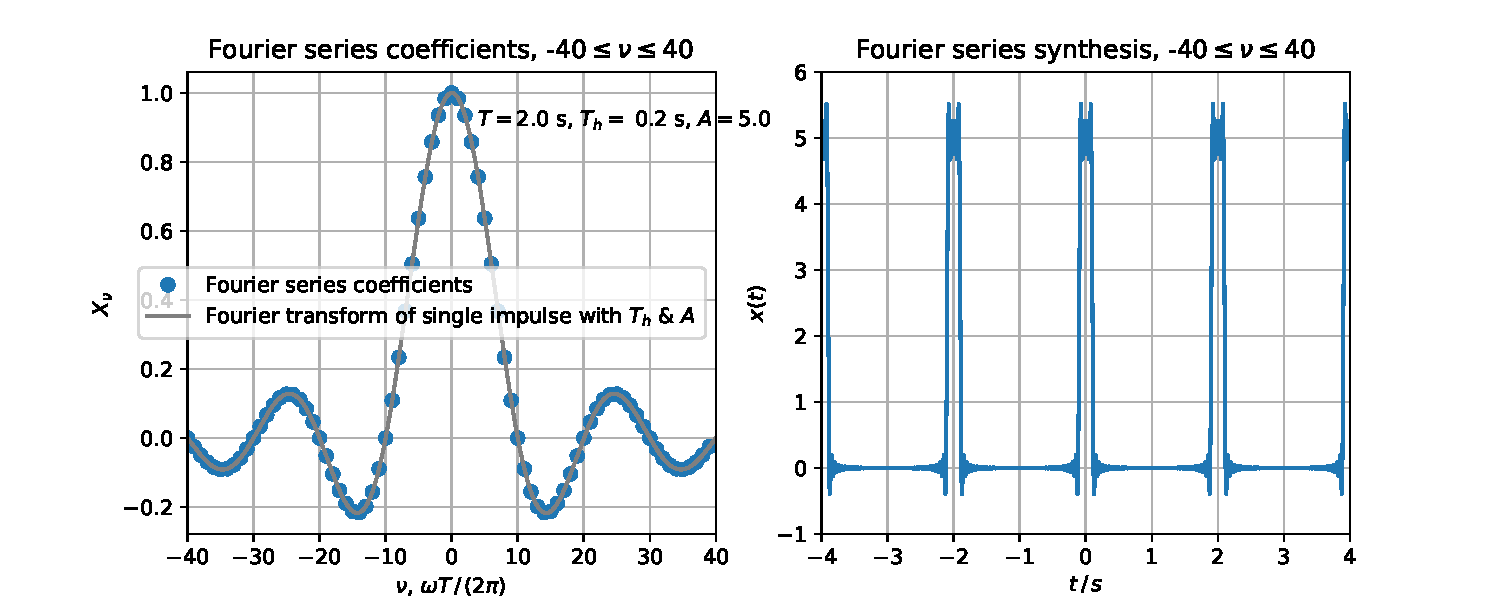
\includegraphics[width=\textwidth]{../fs/D1483A84E2_0.pdf}
\caption{Koeffizienten der komplexen Fourierreihe $X_\nu$ (links) und Synthese $x(t)$ (rechts) für
$T=2$ s, $T_h=0.2$ s, $A=1/T_h$. \texttt{FourierSeries\_D1483A84E2.ipynb}}
\label{fig:D1483A84E2_0}
\end{figure}

\begin{figure}
\includegraphics[width=\textwidth]{../fs/D1483A84E2_1.pdf}
\caption{Koeffizienten der komplexen Fourierreihe $X_\nu$ (links) und Synthese $x(t)$ (rechts) für
$T=2$ s, $T_h=0.4$ s, $A=1/T_h$. \texttt{FourierSeries\_D1483A84E2.ipynb}}
\label{fig:D1483A84E2_1}
\end{figure}

\begin{figure}
\includegraphics[width=\textwidth]{../fs/D1483A84E2_2.pdf}
\caption{Koeffizienten der komplexen Fourierreihe $X_\nu$ (links) und Synthese $x(t)$ (rechts) für
$T=2$ s, $T_h=1$ s, $A=1/T_h$. \texttt{FourierSeries\_D1483A84E2.ipynb}}
\label{fig:D1483A84E2_2}
\end{figure}

\begin{figure}
\includegraphics[width=\textwidth]{../fs/D1483A84E2_3.pdf}
\caption{Koeffizienten der komplexen Fourierreihe $X_\nu$ (links) und Synthese $x(t)$ (rechts) für
$T=2$ s, $T_h=1.6$ s, $A=1/T_h$. \texttt{FourierSeries\_D1483A84E2.ipynb}}
\label{fig:D1483A84E2_3}
\end{figure}

\begin{figure}
\includegraphics[width=\textwidth]{../fs/D1483A84E2_4.pdf}
\caption{Koeffizienten der komplexen Fourierreihe $X_\nu$ (links) und Synthese $x(t)$ (rechts) für
$T=2$ s, $T_h=2$ s, $A=1/T_h$. \texttt{FourierSeries\_D1483A84E2.ipynb}. Extremfall: für die
Darstellung eines Gleichanteils braucht es nur $X_{\nu=0}$, alle anderen Fourier Koeffizienten
$X_{\nu \neq 0}=0$, weil ja nichts schwingt.}
\label{fig:D1483A84E2_4}
\end{figure}











\cleardoublepage
\subsection{Dirac-Impuls}
\label{sec:D410BDAAE0}
\begin{Ziel}
Wir führen den Dirac-Impuls $\delta(t)$ ein.
Ohne den geht in SigSys (fast) nix, bekannt auch als
Dirac-Delta-Impuls, Dirac-Stoß, Einheitsimpuls.
Wir werden den Dirac-Impuls bei der Beschreibung von Signalen und Systemen
in fundamentalen Zusammenhängen benutzen (müssen).
Wir haben mit der vorigen Aufgabe ganz gut vorgearbeitet und können uns
mit der Rechteck- und Spaltfunktion dem Phänomen Dirac-Impuls nähern.
Ingenieur*innen ist das Konzept am Anfang ein wenig fremd, weil
der Dirac-Impuls keine klassische Funktion ist, sondern eine Distribution, d.h.
es gibt bestimmte Funktionen, für die ein eigentlich gewünschter Grenzwert zwar nicht existiert,
die aber gleiche Grundeigenschaften besitzen, wenn man sich dieser Grenze annähert.
Diese Grundeigenschaften werden wir kennenlernen als sehr nützliche
Rechenregeln des Dirac-Impulses, und damit haben wir eigentlich das nötige
Handwerkszeug für SigSys dann schon parat.
Die Rechteck- und Spaltfunktion sind zwei solche Funktionen mit
Grundeigenschaften die einen Dirac-Impuls ausmachen (ganz streng genommen erfüllt
die Rechteckfunktion bestimmte Anforderungen der Distributionstheorie gar nicht,
aber es ist in SigSys-Büchern das deutlich beliebtere Signal einen Dirac Impuls
Grenzübergang aufzuzeigen.)

Zudem werden wir zwei fundamentale Korrespondenzen der Fouriertransformation
kennenlernen, nämlich die des Dirac-Impulses und die des Gleichsignals, das als
weiter Vorgriff auf das was uns erwartet in SigSys.
\end{Ziel}
\textbf{Aufgabe} {\tiny D410BDAAE0}:
Finden Sie $x(t)=\delta(t)\quad \fourier \quad X(\omega)=?$ sowie
$x(t)= ? \quad \fourier \quad X(\omega)=2\pi \delta(\omega)$
\begin{Werkzeug}
Führen wir für $\xi\in\mathbb{N}^+$ eine Funktion $\delta_\xi(t)$ ein, die entweder
\begin{equation}
\delta_\xi(t) := \xi \cdot \mathrm{rect}(\xi \, t) =
\begin{cases} \xi & |t| < \frac{1}{2 \xi} \\ \frac{\xi}{2} & |t| = \frac{1}{2 \xi} \\ 0 & |t| > \frac{1}{2 \xi} \end{cases}\quad
\end{equation}
oder
\begin{equation}
\delta_\xi(t) := \frac{\xi}{\pi} \cdot \mathrm{sinc}(\xi \, t) = \frac{\sin(\xi \, t)}{\pi t}
\end{equation}
ist.
Wir entdecken die---zwar ein wenig normiert aber uns mittlerweile vertraute---
Rechteck- und Spaltfunktion wieder.
%
Es gilt für beide Funktion, und zwar unabhängig von $\xi$ (für die
Rechteckfunktion ist das leicht einzusehen, für die sinc-Funktion überlassen wir
das den Mathematiker*innen und/oder müssen uns vertiefter mit dem Integralsinus
auseinander setzen)
\begin{equation}
\int\limits_{-\infty}^{+\infty} \delta_\xi(t) \fsd t = 1,
\end{equation}
d.h. die \textbf{Fläche ist immer 1} bei der gewählten Normierung der
Rechteck- und Spaltfunktion.
%
Nun sind die Grenzwerte
%\begin{equation}
$\lim_{\xi\to\infty} \delta_\xi(t)$
%\end{equation}
leider nicht definiert, weil die Funktionen wachsen ins Unendliche bei $t=0$.
%
Wir machen uns klar, dass sowohl die Rechteck- als auch Spaltfunktion mit
größer werdendem $\xi\to \infty$ um das Funktionsargument $0$ herum
immer schmaler und höher werden und sich
einem Impuls annähern, siehe \fig{fig:D410BDAAE0}.
%
Die Mathematik\footnote{\url{https://dlmf.nist.gov/1.17} bzw. Bücher wie
\cite[Kapitel 1.11]{Arfken2013}, \cite{Burg2013}}
liefert uns nun eine Lösung im Sinne eines Grenzwerts für eine
Sequenz von Integralen über $\delta_\xi(t)$, $\xi=1,2,3,...$
\begin{equation}
\lim_{\xi\to\infty} \int\limits_{-\infty}^{+\infty}
\delta_\xi(t-t_0) \cdot f(t) \, \fsd t = f(t_0).
\end{equation}
Wir sehen, dass dieser Grenzwert auf eine Funktion $f(t)$ einwirkt und als Lösung
$f(t_0)$ hervorbringt, wenn $\delta_\xi(t)$ um $t_0$ verschoben wurde (der Impuls ist dann bei $t_0$), also
$\delta_\xi(t-t_0)$ im Integral benutzt wurde.
%
Diese Eigenschaft ist das was uns primär in SigSys interessiert.
%
Der für uns etwas sperrige Ausdruck
\begin{equation}
\lim_{\xi\to\infty} \int\limits_{-\infty}^{+\infty}
\delta_\xi(t-t_0) \cdot f(t) \, \fsd t
\end{equation}
bekommt jetzt 'einfach' eine Definition übergeholfen mit
Einführung des sogenannten Dirac-Impulses $\delta(t)$
\begin{equation}
\label{eq:DiracDistrDef}
\lim_{\xi\to\infty} \int\limits_{-\infty}^{+\infty}
\delta_\xi(t-t_0) \cdot f(t) \, \fsd t
:= \int\limits_{-\infty}^{+\infty} \delta(t-t_0) \cdot f(t) \, \fsd t \stackrel{\mathrm{def}}= f(t_0)
\end{equation}
%
Die rechte Seite ist \textbf{kein} klassisches Riemann-Integral, sondern eine
\textbf{Definition} (nämlich die des Grenzwerts für das linke Integral!,
sollte man nicht vergessen, wird aber oft vergessen ;-) ),
für uns aber eine nützliche \text{Rechenregel} und Grundeigenschaft des
Dirac-Impulses. Diese ist als \textbf{Austasteigenschaft} oder
\textbf{Ausblendeigenschaft} (in englisch sifting property, obacht: nicht shifting)
bekannt. Je nachdem wie wir denken wollen:
Austasten nur des Funktionswertes $f(t_0)$ oder Ausblenden aller Funktionswerte
außer $f(t_0)$.

Aus dieser Rechenregel können wir sofort ableiten, dass
\begin{equation}
\label{}
\int\limits_{-\infty}^{+\infty} \delta(t) \cdot f(t) \, \fsd t = f(0)
\end{equation}
wenn $t_0=0$ gewählt wurde.
%
Weiter finden wir
\begin{equation}
\label{eq:D410BDAAE0_area_like}
\int\limits_{-\infty}^{+\infty} \delta(t) \fsd t = 1
\end{equation}
wenn $f(t)=1$ gewählt wurde.
%
Beide Beziehungen konnten wir nur deswegen so schnell und einfach ableiten, weil
wir die Definition benutzt haben. Wir müssen aber immer klar haben, dass wir
nicht das Integral gelöst, sondern vielmehr die Rechenregel der Austastung
verwendet haben.
%
Die Versuchung \eqref{eq:D410BDAAE0_area_like} als Fläche
des Dirac-Impulses zu interpretieren
ist sehr groß, und wenn wir den Grenzübergang mit der Rechteckfunktion in Gedanken
tatsächlich vollziehen auch nicht falsch, aber wir können das streng genommen
nicht aus dem Definitionsintegral (in Notation der Formelsammlung)
$\int\limits_{-\infty}^{+\infty} \delta(t-\tau) \cdot x(t) \, \fsd t \stackrel{\mathrm{def}}= x(\tau)$
des Dirac-Impulses auslesen.
%
Statt Fläche, sprechen wir deswegen zukünftig vom Gewicht 1 des Dirac-Impulses.

\end{Werkzeug}

\noindent Weil es so fundamental wichtig ist, nochmal kompakt für SigSys.
%
Wir stellen uns einen Impuls vor, der
\begin{align}
\int\limits_{t=-\infty}^{+\infty} \delta(t) \fsd t = 1
\qquad\qquad
\delta(t) =
\begin{cases}
\infty & t=0\\
0  & t \neq 0
\end{cases}
\end{align}
als Eigenschaft haben soll. Mit der zweiten Formel kann man aber schlecht rechnen, daher Distribution, Grenzübergang, Definitionsintegral usw., siehe oben.
Am allerwichtigsten ist
\begin{align}
\delta(t) x(t) = \delta(t) x(0)
\end{align}
und dessen Integral
\begin{align}
\int\limits_{t=-\infty}^{+\infty} \delta(t) x(t) \fsd t= \int\limits_{t=-\infty}^{+\infty}  \delta(t) x(0) \fsd t = x(0) \int\limits_{t=-\infty}^{+\infty} \delta(t) \fsd t = x(0),
\end{align}
also die \textbf{Multiplikationseigenschaft} und die \textbf{Austasteigenschaft}.
Wenn man den Impuls verschiebt, so dass die Spitze bei $\tau$ ist, also
\begin{align}
\int\limits_{t=-\infty}^{+\infty} \delta(t-\tau) \fsd t = 1
\qquad\qquad
\delta(t-\tau) =
\begin{cases}
\infty & t=\tau\\
0  & t \neq \tau
\end{cases}
\end{align}
folgt
\begin{align}
\text{Multiplikationseigenschaft allgemein} & \qquad\delta(t-\tau)\,x(t) = \delta(t-\tau)\,x(\tau)\\
\text{Multiplikationseigenschaft für } \tau=0 & \qquad\delta(t)\,x(t) = \delta(t)\,x(0)\\
\text{Austasteigenschaft I allgemein} & \quad \int\limits_{t=-\infty}^{+\infty} \delta(t-\tau) x(t)\fsd t = x(\tau)\\
\text{Austasteigenschaft I für } \tau=0& \quad \int\limits_{t=-\infty}^{+\infty} \delta(t) x(t)\fsd t = x(0)
\end{align}
%
Die allgemeine Austasteigenschaft I können wir mit einem Variablentausch $t \leftrightarrow \tau$ als
\begin{align}
\int\limits_{\tau=-\infty}^{+\infty} \delta(\tau-t) x(\tau)\fsd \tau = x(t)
\end{align}
schreiben. Der Dirac Impuls ist ein gerades Signal, d.h. es gilt $\delta(t)=\delta(-t)$. Es gilt also auch $\delta(\tau-t)=\delta(-(\tau-t))=\delta(-\tau+t)$ und man kann damit die allgemeine Austasteigenschaft II
\begin{align}
\int\limits_{\tau=-\infty}^{+\infty} \delta(-\tau+t) x(\tau)\fsd \tau = x(t),
\end{align}
aufschreiben, die sich auch in der Formelsammlung findet. Typ I und II sind nützlich für verschiedene Rechenwege. Typ I ist in den meisten Lehrbüchern drin und mutmaßlich am Anfang einfacher zu verdauen. Typ II ist sehr gut geeignet, die Faltung elegant herzuleiten.


\begin{figure}[h!]
\includegraphics[width=\textwidth]{../dirac_impulse_ct/D410BDAAE0.pdf}
  \caption{Rechteck- (oben) und normalisierte Spaltfunktion (unten) unterschiedlicher Breite und Höhe.
  Durch die Normierung auf Fläche 1 verhalten sich Breite und Höhe umgekehrt proportional und
  gehen daher in den Grenzfällen zu einem unendlich kleinem Gleichsignal oder einem unendlich kurzen und hohen
  Impuls über. Diese beiden Funktionen gehen im Grenzfall $\xi\to\infty$
  in einen Dirac-Impuls \eq{eq:DiracDistrDef} über.
  \texttt{dirac\_impulse\_CT\_D410BDAAE0.ipynb}}
  \label{fig:D410BDAAE0}
\end{figure}

\begin{figure}[h!]
\centering
%
\begin{tikzpicture}0
\def\l{-2.5}
\def\r{+2.5}
\draw[->] (-2+\l,0) -- (2+\l,0) node[right] {$t$};
\draw[->] (0+\l,0) -- (0+\l,1.5) node[above] {$x(t)=\delta(t)$};
\draw[->, C0, line width=1mm] (0+\l,0) -- (0+\l,1) node[left] {$(1)$};
\node at (0,1) {$\fourier$};
\draw[->] (-2+\r,0) -- (2+\r,0) node[right] {$\omega$};
\draw[->] (0+\r,0) -- (0+\r,1.5) node[above] {$X(\omega)=1$};
\draw[-, C0, line width=1mm] (-2+\r,1) -- (2+\r,1) node[right] {$1$};
\end{tikzpicture}
%
\begin{tikzpicture}0
\def\l{-2.5}
\def\r{+2.5}
\draw[->] (-2+\l,0) -- (2+\l,0) node[right] {$t$};
\draw[->] (0+\l,0) -- (0+\l,1.5) node[above] {$x(t)=1$};
\draw[-, C0, line width=1mm] (-2+\l,1) node[left] {$1$} -- (2+\l,1);
\node at (0,1) {$\fourier$};
\draw[->] (-2+\r,0) -- (2+\r,0) node[right] {$\omega$};
\draw[->] (0+\r,0) -- (0+\r,1.5) node[above] {$X(\omega)=2\pi\delta(\omega)$};
\draw[->, C0, line width=1mm] (0+\r,0) -- (0+\r,1) node[right] {$(2\pi)$};
\end{tikzpicture}
%
\caption{Korrespondenzen Fouriertransformation: \eq{eq:D410BDAAE0_Loesung1} (oben),
\eq{eq:D410BDAAE0_Loesung2} (unten).}
\label{fig:D410BDAAE0_Korrespondenzen}
\end{figure}



\cleardoublepage
\begin{Ansatz}
Die gesuchte Korrespondenz $x(t)=\delta(t)\quad \fourier \quad X(\omega)=?$
können wir ableiten aus der Ausblendeigenschaft
$\int\limits_{-\infty}^{+\infty} \delta(t-t_0) \cdot f(t) \, \fsd t \stackrel{\mathrm{def}}= f(t_0)$
mit $f(t) = \e^{-\im \omega t}$ und $t_0=0$.
%
Dann bekommt die Ausblendeigenschaft das Aussehen der Fouriertransformation
des Dirac-Impulses
\begin{equation}
X(\omega) = \int\limits_{-\infty}^{+\infty} \delta(t) \cdot \e^{-\im \omega t} \, \fsd t \stackrel{\mathrm{def}}= \e^{-\im \omega \cdot 0} = 1
\end{equation}

Auch die gesuchte Korrespondenz
$x(t)= ? \quad \fourier \quad X(\omega)=2\pi \delta(\omega)$ lässt sich
ableiten aus der Ausblendeigenschaft, diesmal mit der Funktionsvariablen Kreisfrequenz, also mit

$\int\limits_{-\infty}^{+\infty} \delta(\omega-\omega_0) \cdot f(\omega) \, \fsd \omega \stackrel{\mathrm{def}}= f(\omega_0)$
für $f(\omega) = \e^{+\im \omega t}$ (Vorzeichen der inversen Fouriertransformation ist $+$!) und $\omega_0=0$.
%
Dann bekommen wir
\begin{equation}
2\pi \cdot \int\limits_{-\infty}^{+\infty} \delta(\omega) \cdot \e^{+\im \omega t} \, \fsd \omega \stackrel{\mathrm{def}}= 2\pi \cdot \e^{+\im \omega \cdot 0} = 2\pi
\end{equation}
%
Weil bei der inversen Fouriertransformation
\begin{align}
x(t) = \frac{1}{2\pi} \int\limits_{-\infty}^{+\infty} X(\omega) \, \e^{+\im \omega t} \fsd \omega
\end{align}
noch der Faktor $\frac{1}{2\pi}$ berücksichtigt werden muss, erhalten wir
\begin{equation}
x(t) = \int\limits_{-\infty}^{+\infty} \delta(\omega) \cdot \e^{+\im \omega t} \, \fsd \omega \stackrel{\mathrm{def}}= \e^{+\im \omega \cdot 0} = 1
\end{equation}

\end{Ansatz}
%\begin{ExCalc}
%\end{ExCalc}
\begin{Loesung}
Damit haben wir zwei weitere wichtige Korrespondenzen gefunden, in der Formelsammlung
ganz oben auf der Liste:
\begin{align}
\label{eq:D410BDAAE0_Loesung1}
x(t)= \delta(t) &\quad \fourier \quad X(\omega)=1\\
\label{eq:D410BDAAE0_Loesung2}
x(t)= 1 &\quad \fourier \quad X(\omega)=2\pi \delta(\omega)\qquad \text{Dirac mit Gewicht}\,\,2\pi
\end{align}
%
Diese sind in \fig{fig:D410BDAAE0_Korrespondenzen} veranschaulicht.
%
Wesentlich ist, dass ein Dirac-Impuls alle Frequenzen gleich gewichtet enthält
(\fig{fig:D410BDAAE0_Korrespondenzen} oben)
und dass ein Gleichsignal, im Spektrum nur einen Dirac-Impuls bei $\omega=0$ enthält
(\fig{fig:D410BDAAE0_Korrespondenzen} unten).
Weil hier eben nichts schwingt, gibt es nur diesen einen Dirac im Spektrum, welcher den
Gleichanteil repräsentiert.
\end{Loesung}




\begin{mdframed}
\textit{Ausblick:}
%
\\\noindent
Wir haben bisher die Korrespondenzen
\begin{align}
x(t)= \delta(t) &\quad \fourier \quad X(\omega)=1\\
x(t)= 1 &\quad \fourier \quad X(\omega)=2\pi \delta(\omega)\\
x(t - \tau) & \quad \fourier \quad X(\omega) \cdot \e^{-\im\omega \tau}\\
x(t) \cdot \e^{+\im\omega_0 t} & \quad \fourier \quad X(\omega-\omega_0)
\end{align}
kennengelernt.
%
Diese lassen sich nun sinnvoll kombinieren, um weitere Korrespondenzen zu finden,
z.B. ein verschobener Dirac-Impuls im Zeitbereich
\begin{align}
\delta(t-\tau)& \quad \fourier \quad 1 \cdot \e^{-\im\omega \tau}.
\end{align}
Das wird uns in SigSys begleiten: Zeitverschiebung führt zu Phasenänderung im Frequenzbereich.

Oder ein verschobener Dirac-Impuls im Frequenzbereich
\begin{align}
1 \cdot \e^{+\im\omega_0 t} & \quad \fourier \quad 2\pi\delta(\omega-\omega_0),
\end{align}
bedeutet Phasenänderung im Zeitbereich, speziell resultiert eine Multiplikation
mit einer komplexen Schwingung auf das ursprüngliche Gleichsignal $x(t)=1$.
%
In der nächsten Übung wird diese Korrespondenz nochmal näher mit einem
Rechteckzeitsignal beleuchtet. Aus der zeitlichen Begrenzung des Gleichsignals
zum Rechtecksignal resultiert ein Übergang vom Dirac-Impuls zur Spaltfunktion
für die Fouriertransformierte.
\end{mdframed}














\newpage
\subsection{Lineare Differentialgleichungen}
\label{sec:A7BEE9E24E}
%
Zunächst keine Aufgabe, sondern erst ein Ausblick in den Kontext einer mutmaßlichen Wiederholung
gestellt.
Wir betrachten hier einleitend den \textbf{SigSys-Teil: Systemanalyse und -synthese}.
Dafür werden wir die Laplace-Transformation (für zeitkontinuierliche Signale, Systeme)
und die $z$-Transformation (für zeitdiskrete Signale/Systeme) kennenlernen, um
Differentialgleichungen und Differenzengleichungen elegant(er) lösbar zu machen.
%
Signale und Systeme sind natürlich sehr eng verknüpft, die hier aufgespannte
Trennung in Signalanalyse/-synthese vs. Systemanalyse/-synthese
sollten wir daher nicht dogmatisch verfolgen, sondern sie dient als grober
Überblick, was uns in SigSys erwarten wird.

In Mathe haben wir das Konzept der Differentialgleichung (DGL) kennengelernt.
%
Wir haben verschiedene Lösungsmöglichkeiten kennengelernt (Variation
der Konstanten, Variablentrennung, Eigenlösungen und charakteristisches Polynom,
Störgliedansätze, usw.). Erschien uns vielleicht ziemlich wirr, weil rechnen
ja, verstehen eher hm...ja/nein/vielleicht?
Das Buch \cite{Strang2014} und andere von Gilbert Strang
lohnt sich durchzuarbeiten; auch die MIT OCW Vorlesungen von ihm sind sehr zu empfehlen.


Lineare DGL mit konstanten (also \textbf{nicht zeitveränderliche}n) Koeffizienten der
ersten und zweiten Ordnung sind die wichtigsten Vertreter, die wir in SigSys
zunächst brauchen, weil man damit beeindruckend viele Dinge bauen und modellieren
kann, Feder-Masse-Dämpfer und RLC-Schwingkreis sind die beiden Klassiker.
%
In den Grundlagen der E-Technik lernten wir alles erst zu Fuß zu lösen, also
die Wechselstromtechnik und die Einschaltvorgänge an RLC-Schaltungen.
%
Nachrichtentechniker*innen bauen sich aus diesen DGLs sogenannte Filter,
früher analog, heute digital.
%
Regelungstechniker*innen bauen sich im Grunde die gleichen Filter, nennen sie nur
selten Filter, sondern eher Glieder mit z.B. differenzierendem, proportionalem,
integrierendem, usw. Verhalten und bauen dann gerne Systeme mit
Rückkopplungsschleifen, weil sie was regeln wollen.
%
Die Brücke zwischen E-Technik und Nachrichten-/Regelungstechnik (und auch
ganz vielen anderen Disziplinen in denen wir mit Signalen agieren...also
auch Energietechnik und Leistungselektronik, Wellentheorie wie
Akustik, Optik, Hochfrequenztechnik usw.) ist SigSys!

Wir werden uns daher in der SigSys einen eleganten Formalismus erarbeiten,
diesen DGL-Typ für beliebige Störgliedansätze zu lösen (am Ende des Tages
müssen wir ja praktisch vorkommende Signale verarbeiten und können uns nicht
auf schicke, auf Papier lösbare Störgliedformeln beschränken)
und das Konzept der Eigenlösungen und des charakteristischen
Polynoms vertiefen bzw. aus anderem Blickwinkel betrachten (am Ende des Tages
wollen wir für eine bestimmte Aufgabe eine Lösung mit gewünschter Genauigkeit
mit dem einfachsten(!) Aufwand erhalten). Praktisch die gesamte SigSys ist daraufhin
ausgelegt, auch wenn sich das momentan noch nicht so anfühlen mag.

Der folgende Abschnitt soll daher die SigSys Denke ein wenig schmackhaft machen und
greift den didaktisch brillanten Faden aus \cite{Strang2014} auf. Viele Dinge
müssten uns aus der Mathe-VL vertraut vorkommen.
%
Zum Auffrischen sei auch \cite{Burg2013} sehr empfohlen, das ist SigSys aus weiterer
Sicht von Mathematiker*innen.
%
\subsubsection{Lineare DGL 2. Ordnung mit konstanten Koeffizienten}
Betrachten wir beispielhaft die lineare DGL 2. Ordnung
\begin{align}
\label{eq:A7BEE9E24E_DGL}
A \frac{\fsd^2 y(t)}{\fsd t^2} + B \frac{\fsd y(t)}{\fsd t} + C y(t) = x(t),
\end{align}
mit den konstanten Koeffizienten $A,B,C\in\mathbb{R}$.
%
Die DGL stellt ein System dar mit dem Eingangssignal $x(t)$
(das ist die Störfunktion / Anregungsfunktion) und dem Ausgangssignal
$y(t)$ (das ist die Lösung der DGL).
%
In der SigSys Literatur ist die Notation von Eingang $x(t)$ und Ausgang $y(t)$
sehr weit verbreitet, aber wir sind gut beraten das im Detail vorher zu checken.
%
Die Koeffizienten $A,B,C$ bestimmen im Wesen, wie das System den Eingang $x(t)$
im Sinne der ersten und zweiten Ableitung \textbf{linear ändert} zum Ausgang $y(t)$.

Die Lösung der DGL ist immer die Superposition von homogener und partikulärer
Lösung
%
\begin{align}
y(t) = y_h(t) + y_p(t)
\end{align}
mit Berücksichtigung der Anfangsbedingungen meist für exakt $t=0$, also gegebenem
$y(0)$, $y'(0)$.
%
Die homogene Lösung findet alle $y_h(t)$ für den Fall $x(t)=0$.
%
Für das spezielle Eingangssignal $x(t)\neq 0$ in
\eq{eq:A7BEE9E24E_DGL} erhalten wir die partikuläre Lösung $y_p(t)$.
%
\subsubsection{Homogene Lösung: Charakteristisches Polynom}
%
Wir haben gelernt (und vielleicht sogar didaktisch fein hergeleitet bekommen,
warum das so sein muss), dass man die homogene Lösung dieser DGL mit dem
Lösungsansatz
\begin{equation}
y_h(t) \propto \e^{\lambda t}\qquad \lambda\in\mathbb{C}
\end{equation}
erhält ($\propto$ meint proportional zu, dann können wir hier erst einmal
eventuelle Vorfaktoren weglassen).
%
Setzen wir diesen Ansatz in \eq{eq:A7BEE9E24E_DGL} ein, führen die Ableitungen
aus, erhalten wir das \textbf{charakteristische Polynom} in der Klammer von
\begin{equation}
(A \lambda^2 + B \lambda + C) \cdot \e^{\lambda t} = 0
\end{equation}
mit den zwei Lösungen ($\e^{\lambda t}$ bekommen wir nicht zu Null)
\begin{align}
\label{eq:A7BEE9E24E_lambdas}
\lambda_{1,2} = \frac{-B \pm \sqrt{B^2-4 A C}}{2 A},
\end{align}
die
\begin{itemize}
  \item a) reell und unterschiedlich sind, wenn $B^2>4 A C$
  \item b) reell und identisch sind, wenn $B^2 = 4 A C$
  \item c) konjugiert-komplex sind, wenn $B^2<4 A C$.
\end{itemize}
%
Für die Fälle a) und c) gilt immer der Ansatz
\begin{mdframed}[backgroundcolor=C3!10]
\begin{align}
\label{eq:A7BEE9E24E_Eigenloesungen}
y_h(t) = c_1 \e^{\lambda_1 t} + c_2 \e^{\lambda_2 t},
\end{align}
\end{mdframed}
%
Wichtig zu erkennen ist, dass wir---je nachdem wie $\lambda_1$ und $\lambda_2$
beschaffen ist (also abhängig von den Koeffizienten $A,B,C$)---verschiedene
Funktionsverläufe als homogene Lösungen erhalten.
Es ginge:
\begin{itemize}
  \item harmonische komplexe, sin- oder cos-Schwingung (wenn $B=0$, d.h. Resonanz)
  \item gedämpfte komplexe, sin- oder cos-Schwingung
  \item aufklingende komplexe, sin- oder cos-Schwingung (in der Praxis zu vermeiden)
  \item abfallender exponentieller Verlauf
  \item ansteigender exponentieller Verlauf (siehe COVID-19, in der Praxis zu vermeiden).
\end{itemize}
Dies sind \textbf{Eigenlösungen} der homogenen DGL und können mit
\eq{eq:A7BEE9E24E_Eigenloesungen} beschrieben werden.
%
Die noch fehlende Eigenlösung für Fall b) ist $y_h(t) = t \e^{\lambda_1 t}$, das
ist der sogenannte aperiodische Grenzfall (auch bekannt als kritisch bedämpfter Fall)
und bedarf deswegen einer eigenständigen Lösung,
den wir hier zunächst mal vernachlässigen wollen.

\subsubsection{Homogene Lösung: Eigenwerte und Vektoren der Koeffizientenmatrix}
%
Es ist bemerkenswert, dass die homogenen Lösungen
auch hervorgehen, wenn man Eigenwerte und Eigenvektoren einer ganz bestimmten Matrix
berechnet. Das ist natürlich kein Zufall; und mit diesem Ansatz können wir viele
nützliche Tools aus der linearen Algebra mitverwenden.

Um die Matrix aufzustellen, schreiben wir zunächst die homogene DGL um zu
\begin{align}
\frac{\fsd^2 y(t)}{\fsd t^2} + \frac{B}{A} \frac{\fsd y(t)}{\fsd t} + \frac{C}{A} y(t) = 0.
\end{align}
%
Wir können diese DGL 2. Ordnung nun auch in zwei getrennten DGL aufschreiben. Das wird
der Grundstein für die Matrix-Sichtweise.
%
Mit den gängigen abgekürzten Schreibweisen für Zeitableitung
\begin{align}
\frac{\fsd y(t)}{\fsd t} = y'(t) = \dot{y}
\end{align}
können wir schreiben
\begin{align}
\frac{\fsd^2 y(t)}{\fsd t^2} = \frac{\fsd y'(t)}{\fsd t} = - \frac{B}{A}  \frac{\fsd y(t)}{\fsd t} - \frac{C}{A}  y(t).
\end{align}
%
Diese beiden Gleichungen können wir nun als einfaches Matrix-Gleichungssystem formulieren
\begin{align}
\label{eq:A7BEE9E24E_uAU}
\vec{u}' = \frac{\fsd}{\fsd t}
\begin{bmatrix}
y(t) \\ y'(t)
\end{bmatrix}
=
\begin{bmatrix}
0 & 1 \\ - \frac{C}{A} & - \frac{B}{A}
\end{bmatrix}
\begin{bmatrix}
y(t) \\ y'(t)
\end{bmatrix}
=
\vec{A} \vec{u}.
\end{align}
%
Wir finden in der Matrix $\vec{A}$ alle Koeffizienten $A,B,C$ wieder, daher
ist es sinnvoll diese als Koeffizientenmatrix zu bezeichnen und sich klarzumachen,
dass diese Matrix das System vollständig beschreibt.

Behauptung:
Dieses Gleichungssystem lässt sich mittels Eigenwert $\lambda$ und passendem
Eigenvektor $\vec{x}$ lösen, also
\begin{align}
\vec{A} \vec{x} = \lambda \vec{x},
\end{align}
wobei es kein Zufall ist, dass wir auch hier die Variable $\lambda$, wie schon
beim charakteristischen Polynom verwenden: es sind die gleichen Zahlen.
Wir wissen, dass man die unbekannten Eigenwerte mittels Ansatz
$(\vec{A} - \lambda \vec{I})\vec{x} = \vec{0}$, also singulärer Matrix
$(\vec{A} - \lambda \vec{I})$, also $\mathrm{det}(\vec{A} - \lambda \vec{I})=0$
findet.
%
Daher
\begin{align}
\vec{A} - \lambda \vec{I} =
\begin{bmatrix}
0 & 1 \\ -\frac{C}{A} & -\frac{B}{A}
\end{bmatrix}
-\lambda
\begin{bmatrix}
1 & 0 \\ 0 & 1
\end{bmatrix}
=
\begin{bmatrix}
-\lambda & 1 \\ -\frac{C}{A} & -\frac{B}{A} - \lambda
\end{bmatrix}
\end{align}
und derer Determinante
\begin{align}
-\lambda \cdot (-\frac{B}{A} - \lambda) - (-\frac{C}{A})\cdot 1 = \lambda^2 + \frac{B}{A} \lambda + \frac{C}{A}.
\end{align}
%
$\mathrm{det}(\vec{A} - \lambda \vec{I})=0$ wird also zu
\begin{align}
A \lambda^2 + B \lambda + C = 0
\end{align}
mit den \textbf{zwei Eigenwerten} $\lambda_{1,2}$ aus \eq{eq:A7BEE9E24E_lambdas},
weil genau nicht zufällig, exakt identisch mit dem charakteristischen Polynom.
%
Für die beiden zugehörigen Eigenvektoren $\vec{x}_{1}$ und $\vec{x}_{2}$ finden sich wegen
dem geforderten
\begin{align}
(\vec{A} - \lambda_{1,2} \vec{I}) \, \vec{x}_{1,2} = \vec{0}
\end{align}
die Lösungen
\begin{align}
\vec{x}_{1,2} =
\begin{bmatrix}
1 \\ \lambda_{1,2}
\end{bmatrix}.
\end{align}
%
Wir schreiben für $\vec{A} \vec{x} = \lambda \vec{x}$
%
\begin{align}
\vec{A}
\begin{bmatrix}
1 \\ \lambda_{1,2}
\end{bmatrix} = \lambda_{1,2}
\begin{bmatrix}
1 \\ \lambda_{1,2}
\end{bmatrix},
\end{align}
%
mit
\begin{align}
\lambda_{1,2} = \frac{-B \pm \sqrt{B^2-4 A C}}{2 A}.
\end{align}
%
Wichtig: das gerade beschriebene Vorgehen funktioniert nur, wenn
$\lambda_1 \neq \lambda_2$, also tatsächlich zwei unabhängige Eigenvektoren vorliegen.
%
$\lambda_1 = \lambda_2$ ist wieder der Spezialfall des aperiodischen Grenzfalls.

Unser Ausgangspunkt war $\vec{A}  \vec{u} = \vec{u}'$ in \eq{eq:A7BEE9E24E_uAU}.
Wie verknüpfen wir das mit der gefundenen Eigenwert/-vektor-Darstellung?
%
Kein stringenter Beweis, aber fundamentale Beobachtung
(weil wir damit das Fundamentalsystem neu erfinden), nämlich
$\frac{\fsd \e^{a t}}{\fsd t} = a \e^{a t}$.
%
Es ist nicht verboten zu erweitern
\begin{align}
\vec{A}
\begin{bmatrix}
1 \\ \lambda_{1,2}
\end{bmatrix}
\e^{\lambda_{1,2} t}
= \lambda_{1,2}
\begin{bmatrix}
1 \\ \lambda_{1,2}
\end{bmatrix}
\e^{\lambda_{1,2} t}
\end{align}
und wir sehen, dass wenn wir
\begin{align}
\vec{u}_{1,2} = \vec{x}_{1,2} \cdot \e^{\lambda_{1,2} t}
\end{align}
definieren, die Gleichung \eq{eq:A7BEE9E24E_uAU} dann aufgeht, weil bei der Ableitung zu
$\vec{u}'_{1,2}$ der benötigte Vorfaktor $\lambda_{1,2}$ entsteht.
%
$\vec{x}_{1,2}$ ist also im Grunde zeitbereinigt, enthält aber als Eigenvektor
alle Informationen, die wir brauchen, um das Systemverhalten zu beschreiben.
%
$\vec{u}_{1,2}$ ist dann die Version, wo die zeitliche Änderung mittels
$\e^{\lambda_{1,2} t}$ berücksichtigt ist.
%
Das gewünschte Gleichungssystem $\vec{u}'=\vec{A}  \vec{u}$ kann nun einfach
gelöst werden:
%
Die Linearkombination aller (hier der beiden) Vektoren $\vec{u}_{1,2}$ ergibt den
Lösungsraum
\begin{mdframed}[backgroundcolor=C3!10]
\begin{align}
\begin{bmatrix}
y(t) \\ y'(t)
\end{bmatrix} =
c_1 \e^{\lambda_1 t}
\begin{bmatrix}
1 \\ \lambda_{1}
\end{bmatrix}
+
c_2 \e^{\lambda_2 t}
\begin{bmatrix}
1 \\ \lambda_{2}
\end{bmatrix},
\end{align}
\end{mdframed}
%
wobei man für die erste Zeile die Lösung $y(t)$ erkennt und für die zweite $y'(t)$
(man erkennt das, aber wir hatten $\vec{u}$ in \eq{eq:A7BEE9E24E_uAU}
eben auch genau so definiert).
%
Wir haben damit die gleiche Lösung der DGL wie beim Rechnen mit dem
charakteristischen Polynom gefunden.
%
Mit dieser homogenen Lösung können wir dann partikuläre Lösungen zum Beispiel mit
Variation der Konstanten berechnen.

Soweit der kurze Abriss mit hoffentlich wiederholendem Charakter.
%
Wir machen weiter mit einem fundamentalen Zusammenhang, der die Grundlage der
SigSys-Theorie für linear Systeme (also lineare DGL mit konstanten Koeffizienten)
ist.
%
Keine Sorge, wenn das folgende ein wenig sperrige Kost ist, es ist mutmaßlich
Neuland, aber der Teaser hier ist wichtig, damit wir ein Gefühl für das Wesen von SigSys
bekommen.

\subsubsection{Spezielle Anregung mit Dirac-Impuls}
\label{sec:Spezielle_Anregung_mit_Dirac_Impuls}
Wir betrachten die homogene Lösung unter einer bestimmten Anfangsbedingung
(vgl. \cite[S.97]{Strang2014})
\begin{align}
A y''(t) + B y'(t) + C y(t) = 0,\quad y(0)=0,\quad y'(0)=\frac{1}{A}.
\end{align}
%
Immer noch nur für $\lambda_1 \neq \lambda_2$ ! wissen wir von oben
\begin{align}
y_h(t) = c_1 \e^{\lambda_1 t} + c_2 \e^{\lambda_2 t},\qquad
y_h'(t) = c_1 \lambda_1 \, \e^{\lambda_1 t} + c_2 \lambda_2 \, \e^{\lambda_2 t}
\end{align}
und mit $y_p=0$ wird für $y=y_h+y_p=y_h$.
Die Anfangsbedingungen berücksichtigt
\begin{align}
y(0) = c_1 + c_2 = 0,\qquad
y'(0) = c_1 \lambda_1 + c_2 \lambda_2 = \frac{1}{A}
\end{align}
Daraus folgt
\begin{equation}
c_1 = -c_2 = \frac{1}{A} \, \frac{1}{\lambda_1 - \lambda_2}
\end{equation}
und diese Koeffizienten eingesetzt
\begin{align}
\label{sec:A7BEE9E24E_hyh}
y(t) =
\frac{1}{A} \, \frac{\e^{\lambda_1 t} - \e^{\lambda_2 t}}{\lambda_1 - \lambda_2}.
\end{align}
%
Soweit, so gut. Schaut aus wie just another Lösung, aber diese hat es in sich:
%

Erinnern wir uns an den Dirac-Impuls aus Aufgabe \ref{sec:D410BDAAE0},
den unendlich hohen und schmalen Impuls,
wofür wir Rechenregeln finden mussten, weil eben keine klassische Funktion.
%
Wenn wir diesen Dirac-Impuls als Anregung / Eingang / Störgröße für unsere DGL
wählen und verschwindende Anfangswerte als linksseitigen Grenzwert
berücksichtigen (ruhendes System bis kurz vor der Anregung bei exakt $t=0$), also

\begin{mdframed}[backgroundcolor=C3!10]
\begin{align}
A y''(t) + B y'(t) + C y(t) = \delta(t),\qquad y'(0_-) = 0,\qquad y(0_-) = 0
\end{align}
\end{mdframed}
erhalten wir als Lösung exakt \eq{sec:A7BEE9E24E_hyh}!
%\begin{align}
%\label{sec:A7BEE9E24E_hyp}
%y(t) =
%\frac{1}{A} \, \frac{\e^{\lambda_1 t} - \e^{\lambda_2 t}}{\lambda_1 - \lambda_2}.
%\end{align}
%
Die Rechnung schauen wir uns zu einem späteren Zeitpunkt an. Es gelingt mit Variation
der Konstanten und Benutzung der Austasteigenschaft des Dirac Impulses,
vgl. \cite[S.133ff]{Strang2014}.
%
Auch das warum schauen wir uns später an. Wir stellen hier zunächst fest, dass:
homogene DGL mit speziellen Anfangsbedingungen zu $t=0$ ist gleich wie
Lösung der Anregung mit Dirac-Impuls $\delta(t)$ zum Zeitpunkt $t=0$ mit
linksseitigen, verschwindenden Anfangsbedingungen.

In SigSys bezeichnen wir diese Lösung als \textbf{Impulsantwort} $h(t)$
eines Systems (das ist die Antwort der Systembeschreibung mittels DGL auf den
Dirac Impuls mit Gewicht 1, Mathematiker*innen
bezeichnen diese Lösung gerne auch als \textbf{Green'sche Funktion})
\begin{mdframed}[backgroundcolor=C3!10]
\begin{align}
h(t) =
\frac{1}{A}\,\frac{\e^{\lambda_1 t} - \e^{\lambda_2 t}}{\lambda_1 - \lambda_2}
\qquad \lambda_1 \neq \lambda_2.
\end{align}
\end{mdframed}

%\newpage
Mit dieser können wir die \textbf{partikuläre Lösung jeder beliebigen Anregung},
also Störfunktion $x(t)$ angeben, und zwar mit dem sogenannten
\textbf{Faltungsintegral} beginnend ab unserem hier gewähltem
Zeitpunkt $t=0$
%
\begin{mdframed}[backgroundcolor=C3!10]
\begin{equation}
y_p(t) = \int\limits_{\tau=0}^{t} h(t-\tau) x(\tau) \fsd \tau
\end{equation}
\end{mdframed}
%
Falls das System vorher in Ruhe war, ist dies auch die komplette Lösung $y(t)$.
%

Wir finden dieses Faltungsintegral (mit allgemeineren Grenzen) in der
Formelsammlung in dem Abschnitt Faltung, da die Operation allgemeingültig als
\textbf{Faltung} bekannt ist.
%
Für einen Zeitpunkt $t$ werden alle Beiträge der Eingangsgröße $x$ mit der Impulsantwort $h$
gewichtet und \textit{addiert}. Bezüglich eines Zeitpunkts $t$, werden \textit{aktuelle}
Eingangswerte $x(t)$ mit dem \textit{Anfang} der Impulsantwort, \textit{lange}
zurückliegende Eingangswerte mit dem \textit{Ende} der Impulsantwort gewichtet.
%
Wir werden das bald im Detail lernen, es ist ein ganz wesentliches Integral und
eine ganz wesentliche Operation und deswegen \textbf{immer klausurrelevant}.
%
Machen wir uns nochmal klar: in $h(t)$ steckt die Systeminformation in Form
der Eigenwerte $\lambda_{1,2}$, also am Ende des Tages in Form der Koeffizienten $A,B,C$.
Die zeitliche Komponente ist durch $\e^{\lambda_{1,2} t}$ abgebildet.

Der hier nicht näher betrachtete aperiodische Grenzfall $\lambda_1 = \lambda_2$
hat eine eigene Impulsantwort $h(t) \propto t \e^{\lambda t}$.
%
Das Faltungsintegral gilt aber konsistent
für alle Fälle a), b), c). Das Integral weiß ja nicht und interessiert sich auch nicht,
dass wir eine Funktion als Impulsantwort auffassen und wir Fallunterscheidungen
vornehmen müssen, je nachdem wie $A$, $B$ und $C$ beschaffen sind.

Wir fragen uns jetzt zu Recht, ob das Faltungsintegral
uns das Leben so viel einfacher macht, als DGLs zu lösen, so wie wir das in Mathe
gelernt haben.
%
Unbedingt ja! Deswegen gehört die SigSys zum Grundausbildungskanon für angehende
Ingenieur*innen.
Es erhellt erstens, was bei DGLs eigentlich passiert, die Rechnerei
ist nicht notwendigerweise einfacher geworden, aber wir werden zweitens mit der
\textbf{Laplace Transformation} eine
Methode kennenlernen diese ganze \textbf{DGL-Rechnerei und Faltungsoperation auf
einfache algebraische Funktionen runterzubrechen}. Aus der Faltung von zwei
Zeitfunktionen wird dann die Multiplikation zweier Laplace Transformierter.
%
Die Laplace Transformierte der Impulsantwort enthält viele Informationen auf
sehr übersichtliche Weise und ist perfekt für die tägliche Ingenieurarbeit, sei
es in der Regelungstechnik, Kommunikationstechnik oder Maschinenbau, Mechatronik.

\newpage
\subsection{Aufgabe: Homogene Lösung einer DGL 2. Ordnung mit konstanten
Koeffizienten und Anfangsbedingungen}
\label{sec:A7BEE9E24E_Aufgabe}
\begin{Ziel}
Anhand eines speziellen (wiederkehrenden) Beispieles, wollen wir die Impulsantwort berechnen. Auch,
wenn wir unsere Lösung jetzt noch nicht anderweitig verifizieren können,
ist es sinnvoll hier nochmal eine DGL zu lösen und dann gleich einen sehr wichtigen
Spezialfall.
\end{Ziel}
\textbf{Aufgabe} {\tiny A7BEE9E24E}: Berechnen Sie für die DGL 2. Ordnung
\begin{align}
\frac{16}{25} \ddot{y}(t) + \frac{24}{25} \dot{y}(t) + y(t) = 0,
\quad \dot{y}(0)=\frac{25}{16}, \quad y(0)=0.
\end{align}
die Lösung $y(t)$ für $t\geq 0$.
\begin{Werkzeug}
Entweder wir benutzen die Sachen aus dem vorangegangen Repetitorium Abschnitt
\ref{sec:A7BEE9E24E} oder
wir befragen unsere Mathe-Vorlesungsunterlagen. Ziel soll zunächst sein, diese
DGL korrekt zu lösen.
\end{Werkzeug}
\begin{Ansatz}
Im github Repository

\url{https://github.com/spatialaudio/signals-and-systems-exercises}

findet sich im Ordner

\verb|tutorial_extended_latex_deu|

im LaTex Skript (pdf liegt im StudIP)

\verb|laplace_transform/laplace_transform_839973EF5D.tex| eine

ausführlichste Lösung.
Dieses Dokument bekommt ab ca. der Mitte des Semesters Relevanz.
\end{Ansatz}
%\begin{ExCalc}
%\end{ExCalc}
\begin{Loesung}
Wir sollten zur Lösung
\begin{align}
y(t) = \frac{25}{16} \e^{-\frac{3}{4} t} \sin(t), \qquad t\geq 0
\end{align}
gelangen.
%
Dies ist eine Sinusschwingung die exponentiell gedämpft wird und mit
$\frac{25}{16}$ gewichtet ist.
Wegen des gestellten Problems haben wir die Impulsantwort dieser DGL berechnet.
\end{Loesung}
  % Einführung, FS, FT, Dirac, ODE2nd, h(t)

%\setcounter{section}{1}
%%------------------------------------------------------------------------------
\newpage
\section{UE 2: Elementarsignale- und Operationen, LTI-System Eigenschaften, Faltung}
\label{sec:ue2_faltung}

Wir müssen uns zunächst mit den zeitkontinuierlichen Elementarsignalen vertraut
machen, siehe \verb|fundamental_signals_CT.pdf| im StudIP unter Formelsammlung.

Diese sind
\begin{itemize}
  \item Exponentialfunktion
  $\e^{s_0 \, t}$ mit $s=\sigma_0 + \im\omega_0, s_0\in\mathbb{C}, \sigma_0\in\mathbb{R}, \omega_0\in\mathbb{R}$
  \item Rechtecksignal $\mathrm{rect}(t)$ (Konvention: Fläche 1)
  \item Dreiecksignal $\mathrm{tri}(t)$  (Konvention: Fläche 1)
  \item Spaltfunktion $\mathrm{sinc}(t):=\frac{\sin t}{t}$
  \item Sprungfunktion $\epsilon(t)$
  \item Vorzeichenfunktion $\mathrm{sgn}(t)$
  \item Dirac Impuls $\delta(t)$
  \item Dirac Impuls Kamm $\Sha$(t)
\end{itemize}
\red{TBD mit tikz / pgfplots}








\newpage
\subsection{Signaloperationen: Verschiebung und Skalierung}
\label{sec:42DE8C69F7}
\begin{Ziel}
Es ist wichtig, dass wir uns für die Zeitfunktion $f(t)$
die Operationen
Zeitverschiebung,
Zeitskalierung und die Amplitudenskalierung, also
$A \cdot f(\left[t-\tau\right]\cdot \theta)$ mit $A,\tau,\theta\in\mathbb{R}$
klarmachen.
%
Wie man so schön sagt, müssen wir das für SigSys im Schlaf beherrschen.
\end{Ziel}
\textbf{Aufgabe} {\tiny 42DE8C69F7}: Stellen Sie
{$x(t) = \frac{3}{4} \cdot \mathrm{rect}(\frac{1}{3} t-\frac{1}{2})$}
grafisch dar.
\begin{Werkzeug}
Für
\begin{equation}
A \cdot f(\left[t-\tau\right]\cdot \theta)  \qquad A,\tau,\theta\in\mathbb{R}
\end{equation}
gilt
\begin{itemize}
  \item Zeitverschiebung mit
  $\tau$: für $\tau>0$ verzögert, rechtsverschoben; für $\tau<0$ vorauseilend, linksverschoben
  \item Zeitskalierung mit $\theta$: für $\theta>1$ Stauchung; für $0<\theta<1$ Streckung
  \item Amplitudenskalierung mit $A$: für $0<|A|<1$ Stauchung, für $|A|>1$ Streckung
  \item (für $A<0$ zusätzlich noch Invertieren der Signalpolarität)
  \item (für $\theta<0$ zusätzlich noch Invertieren des Zeitverlaufs)
\end{itemize}
\end{Werkzeug}
\begin{Ansatz}
Es ist sinnvoll, das Signal in die Darstellung
\begin{equation}
x(t) = \frac{3}{4} \cdot \mathrm{rect}(\left[t-\frac{3}{2}\right]\cdot \frac{1}{3})
\end{equation}
umzuformen, weil dann $t$ ohne Vorfaktor und so wie obige Formel.
Dann lässt sich Zeitverschiebung und Zeitskalierung
getrennt und nacheinander abarbeiten. Hier also zunächst Zeitverzögerung um
$\frac{3}{2}$ und dann zeitliche Streckung (das Signal wird 'langsamer' bzw.
braucht über die Zeit länger) mit $\frac{1}{3}$.
%
Zum Schluss noch die Amplitudenstauchung auf Amplitude $1 \cdot \frac{3}{4}$.
%
Es ist empfehlenswert, sich das kochrezeptartig anzugewöhnen, bis es sitzt.

Bei einem cos()-Signal leuchtet uns die zeitliche Streckung, Stauchung vielleicht
intuitiv ein: ausgehend von $\cos(t)$ schwingt $\cos(2\,t)$ schneller, das ist eine
zeitliche Stauchung.
%
Jedoch ausgehend von $\cos(t)$ schwingt $\cos(\frac{1}{2}\,t)$
langsamer, das ist dann eine zeitliche Streckung.

Machen wir uns klar, dass wir auch eine Verschiebung des Signals bezüglich der
Ordinate vornehmen können. Das heißt wir manipulieren den Gleichanteil.
%
Signale mit Gleichanteil werden in den meisten signallastigen
Ingenieursdisziplinen vermieden, weil man den Gleichanteil schlecht
(elektrische Dauerlast, Wärme) oder gar nicht (z.B. Gleichstrom über Luft?!)
übertragen kann.
%
Wir benutzen das daher in den SigSys-UE seltener.

\end{Ansatz}
%\begin{ExCalc}
%\end{ExCalc}
\begin{Loesung}
Das Signal ist in \fig{fig:42DE8C69F7}d dargestellt. Der Lösungsweg folgt von
\fig{fig:42DE8C69F7}a zu \fig{fig:42DE8C69F7}d.

Eine gute Kontrollmöglichkeit bietet Wolfram Alpha
\url{https://www.wolframalpha.com/}.
Nachdem wir uns vergewissert haben, dass die Rechteckfunktion dort ähnlich definiert
ist (Breite, Höhe, Fläche ist jeweils 1), können wir
\verb|3/4*rect(1/3*t-1/2)| eingeben und bekommen eine analytische und grafische
Lösung von Wolfram Alpha angeboten.
Hinweis: die Sprungfunktion erhalten wir mit \verb|step(t)|
und die Dreieckfunktion mit \verb|tri(t)|, damit können wir eigene einfache
Experimente zur Signalskalierung und -verschiebung machen.
%
Das sollten wir in jedem Fall mal machen in einer Mußestunde!

%Mit UE 1.1 aus dem SS2019 können wir noch mehr üben.
\end{Loesung}

\begin{figure*}[h!]
\centering
\begin{subfigure}{0.45\textwidth}
\begin{tikzpicture}
\begin{axis}[
width=1\textwidth,
height=0.5\textwidth,
domain=-4:4,
samples=50,
legend pos=outer north east,
xlabel = {t},
%ylabel = {x(t)},
title = {$x(t) = \mathrm{rect}(t)$},
xmin=-4, xmax=4,
ymin=-0.1, ymax=1.1,
xtick={-4,-3,-2,-1,0,1,2,3,4},
ytick={0,0.5,1,1.5,2},
ymajorgrids=true,
xmajorgrids=true
]
\addplot[mark=None, color=C0, ultra thick]
coordinates {(-4,0)(-1/2,0)(-1/2,1)(1/2,1)(1/2,0)(4,0)};
\end{axis}
\end{tikzpicture}
\caption{Elementarsignal Rechteckfunktion.}
%\label{fig:}
\end{subfigure}
%
\begin{subfigure}{0.45\textwidth}
\begin{tikzpicture}
\begin{axis}[
width=1\textwidth,
height=0.5\textwidth,
domain=-4:4,
samples=50,
legend pos=outer north east,
xlabel = {t},
%ylabel = {x(t)},
title = {$x(t) = \mathrm{rect}(t-\frac{3}{2})$},
xmin=-4, xmax=4,
ymin=-0.1, ymax=1.1,
xtick={-4,-3,-2,-1,0,1,2,3,4},
ytick={0,0.5,1,1.5,2},
ymajorgrids=true,
xmajorgrids=true
]
\addplot[mark=None, color=C0, ultra thick]
coordinates {(-4,0)(1,0)(1,1)(2,1)(2,0)(4,0)};
\end{axis}
\end{tikzpicture}
\caption{Zeit\textbf{verzögerung}.}
%\label{fig:}
\end{subfigure}


\begin{subfigure}{0.45\textwidth}
\begin{tikzpicture}
\begin{axis}[
width=1\textwidth,
height=0.5\textwidth,
domain=-4:4,
samples=50,
legend pos=outer north east,
xlabel = {t},
%ylabel = {x(t)},
title = {$x(t) = \mathrm{rect}(\left[t-\frac{3}{2}\right]\cdot \frac{1}{3}) = \mathrm{rect}( \frac{t}{3} - \frac{1}{2})$},
xmin=-4, xmax=4,
ymin=-0.1, ymax=1.1,
xtick={-4,-3,-2,-1,0,1,2,3,4},
ytick={0,0.5,1,1.5,2},
ymajorgrids=true,
xmajorgrids=true
]
\addplot[mark=None, color=C0, ultra thick]
coordinates {(-4,0)(0,0)(0,1)(3,1)(3,0)(4,0)};
\end{axis}
\end{tikzpicture}
\caption{Zeitverzögerung und -\textbf{streckung}.}
%\label{fig:}
\end{subfigure}
%
\begin{subfigure}{0.45\textwidth}
\begin{tikzpicture}
\begin{axis}[
width=1\textwidth,
height=0.5\textwidth,
domain=-4:4,
samples=50,
legend pos=outer north east,
xlabel = {t},
%ylabel = {x(t)},
title = {$x(t) = \frac{3}{4} \cdot \mathrm{rect}(\left[t-\frac{3}{2}\right]\cdot \frac{1}{3})$},
xmin=-4, xmax=4,
ymin=-0.1, ymax=1.1,
xtick={-4,-3,-2,-1,0,1,2,3,4},
ytick={0,0.5,1,1.5,2},
ymajorgrids=true,
xmajorgrids=true
]
\addplot[mark=None, color=C0, ultra thick]
coordinates {(-4,0)(0,0)(0,3/4)(3,3/4)(3,0)(4,0)};
\end{axis}
\end{tikzpicture}
\caption{Zeitverzögerung/-streckung, \textbf{Amplitudenstauchung}.}
%\label{fig:}
\end{subfigure}
%
%
%
\caption{Skizzenfahrplan für Aufgabe \ref{sec:42DE8C69F7}.
\red{TBD: ipnyb}}
\label{fig:42DE8C69F7}
\end{figure*}





\newpage
\subsection{Ableitung eines Cosinus-Signalausschnitts}
\label{sec:114F06AFAA}
\begin{Ziel}
Wir wollen ein paar prototypische
Rechenmuster der SigSys kennenlernen. Dabei begegnen uns neben ganz normalem
Mathematik-Tools ein paar SigSys-Eigenheiten, die wir in den ersten Vorlesungen und Übungen
erarbeiten, also Standardsignale und deren Zusammenhänge und Eigenschaften.
\end{Ziel}
\textbf{Aufgabe} {\tiny 114F06AFAA}:
Gegeben ist das skizzierte Signal $x(t)$. Finden Sie einen analytisch geschlossenen
Ausdruck für $x(t)$ mit Hilfe von Elementarsignalen. Berechnen Sie die zeitliche
Ableitung $x'(t)$ und stellen Sie diese grafisch dar.
\begin{center}
\begin{tikzpicture}[scale=0.8]
\def \xmin {-4}
\def \xmax {4.2}
\def \ymin {-1}
\def \ymax {1.5}
\draw[->] (\xmin-0.1 ,0) -- (\xmax+0.1,0) node[below]{$t$};
\draw[->] (0,\ymin-0.1) -- (0,\ymax+0.1) node[left]{$x(t)$};
\foreach \x in {\xmin,...,3}{\draw (\x,0.05) -- (\x,-0.05);}
\draw (0.05,-1) -- (-0.05,-1);
\draw (0.05,1) -- (-0.05,1) node[left]{\small $1$};
\draw(2,0) node[below]{\small $2$};
\begin{scope}
\draw[C0, ultra thick, domain=-2:2,variable=\t,samples=100,smooth] plot(\t,{ cos (4*pi*\t r)});
\draw[C0, ultra thick] (-4,0) -- (-2,0);
\draw[C0, ultra thick] (2,0) -- (4,0);
\draw[C0, dashed, thin] (2,0) -- (2,1);
\draw[C0, dashed, thin] (-2,0) -- (-2,1);
\end{scope}
\end{tikzpicture}
\end{center}

\begin{Werkzeug}
Rechteckfunktion, Skalierung, Zerlegung in Sprungfunktionen, Ableitung

Ausblendeigenschaft / Austasteigenschaft des Dirac-Impulses,
was ja eigentlich eher eine Definition, anstatt eine Eigenschaft ist (siehe Übung~\ref{sec:ue1_intro} (1))
\begin{equation}
\int\limits_{-\infty}^{+\infty} \delta(t-\tau) \cdot f(t) \, \fsd t \stackrel{\mathrm{def}}= f(\tau)
\end{equation}

Multiplikationseigenschaft des Dirac-Impulses
\begin{align}
&\delta(t-\tau) f(t) = \delta(t-\tau) f(\tau)\\
&\delta(t) f(t) = \delta(t) f(0) \qquad \text{speziell für} \qquad \tau=0
\end{align}

\end{Werkzeug}
\begin{Ansatz}
Typische SigSys-Denke: Zeitlich begrenzten Cosinus herstellen indem wir mit der
Rechteckfunktion einen Teil ausschneiden. Dann Mathematik betreiben.
\end{Ansatz}
\begin{ExCalc}
Vier Schwingungen pro 2 Sekunden, also Frequenz $f=2$ Hz, also Kreisfrequenz
$\omega=2\pi\cdot 2 = 4\pi$ rad/s, also $\cos(4\pi t)$ (wir haben zeitlich gestaucht)
der nur zwischen $-2 < t < +2$ schwingt. Wir können den Cos dafür mit einer
geeigneten Rechteckfunktion multiplizieren.

Die benötigte Rechteckfunktion muss axialsymmetrisch sein, d.h. es ist keine
Zeitverschiebung involviert.
Die benötigte Rechteckfunktion muss breiter sein, als das Standardsignal
$\mathrm{rect}(t)$, d.h. es ist eine zeitliche Streckung erforderlich.
Breite von $\mathrm{rect}(t)$ ist 1 (hat auch Fläche 1!), wir brauchen aber
Breite 4, daher $\mathrm{rect}(t\cdot \frac{1}{4})$ (zur Erinnerung:
die Funktion soll sich bei Streckung langsamer über der Zeit ändern, daher
Skalierungsfaktor kleiner 1)

Daher kann das Signal als
\begin{align}
x(t) = \cos(4\pi t) \cdot \mathrm{rect}(\frac{t}{4})\\
\end{align}
darstellt werden. Kurzer Check bei Wolfram Alpha bestätigt, dass wir richtig
gerechnet haben.

Für die Zeitableitung
\begin{align}
\frac{\fsd }{\fsd t} x(t) =
\frac{\fsd }{\fsd t} \cos(4\pi t) \cdot \mathrm{rect}(\frac{t}{4})\\
\end{align}
benötigen wir nun die Produkt- und Kettenregel, sowie die Ableitung des Rechtecksignals.

Wir können das Rechtecksignal als Überlagerung von zwei Sprungfunktionen darstellen,
nämlich
\begin{equation}
\mathrm{rect}(\frac{t}{4}) = \epsilon(t+2) -\epsilon(t-2),
\end{equation}
was in der Grafik unten visualisiert ist. Zu besseren Übersichtlichkeit wurden die
Funktionen minimal verschoben/skaliert, damit wir auch bei eigentlicher
Überlappung sehen, wie sie verlaufen. Das Prinzip sollte erkennbar sein.
%
\begin{center}
\begin{tikzpicture}
\begin{axis}[
width=0.5\textwidth,
height=0.3\textwidth,
domain=-4:4,
samples=50,
legend pos=outer north east,
xlabel = {t},
%ylabel = {x(t)},
title = {Rechteckfunktion aus zwei Sprungfunktionen},
xmin=-4, xmax=4,
ymin=-1.1, ymax=1.1,
xtick={-4,-3,-2,-1,0,1,2,3,4},
ytick={-1,-0.5,0,0.5,1},
ymajorgrids=true,
xmajorgrids=true
]
\addplot[mark=None, color=C1, ultra thick]
coordinates {(-4,0.05)(-2,0.05)(-2,1)(4,1)};
\addplot[mark=None, color=C2, ultra thick]
coordinates {(-4,-0.05)(2,-0.05)(2,-1)(4,-1)};
\addplot[mark=None, color=C0, ultra thick]
coordinates {(-4,0)(-1.95,0)(-1.95,0.95)(2,0.95)(2,0)(4,0)};
\legend{$+\epsilon(t+2)$ (vorauseilend),$-\epsilon(t-2)$ (verzögert),$+\epsilon(t+2)-\epsilon(t-2)=\mathrm{rect}(t\cdot\frac{1}{4})$}
\end{axis}
\end{tikzpicture}
\end{center}

Nun brauchen wir folgende wichtige Erkenntnis (die nur indirekt in der Formelsammlung
steht, nämlich bei den Korrespondenzen zur Laplace Transformation) und in
\fig{fig:114F06AFAA} veranschaulicht ist
\begin{equation}
  \epsilon(t)' = \delta(t)
\end{equation}

Damit können wir jetzt ableiten.

Also, zunächst die Zerlegung der Rechteckfunktion in zwei Sprungfunktionen
\begin{align}
\frac{\fsd }{\fsd t} x(t) =
\frac{\fsd }{\fsd t} \cos(4\pi t) \cdot \left( \epsilon(t+2) -\epsilon(t-2)\right)=\\
\frac{\fsd }{\fsd t} \cos(4\pi t) \epsilon(t+2)
- \frac{\fsd }{\fsd t} \cos(4\pi t) \epsilon(t-2)
\end{align}

Ausformulieren bringt
\begin{align}x'(t)=
+ \cos(4\pi t)' \epsilon(t+2) + \cos(4\pi t) \epsilon(t+2)'
- \cos(4\pi t)' \epsilon(t-2) - \cos(4\pi t) \epsilon(t-2)'
\end{align}
\begin{align}x'(t)=
- 4\pi\sin(4\pi t) \epsilon(t+2) + \cos(4\pi t) \delta(t+2)
+ 4\pi\sin(4\pi t) \epsilon(t-2) - \cos(4\pi t) \delta(t-2)
\end{align}
Umsortieren, damit wir aus den Sprüngen wieder eine Rechteckfunktion machen können
(was natürlich nicht immer geht, hier aber zum Glück, weil...?)
\begin{align}x'(t)=
- 4\pi\sin(4\pi t) (\epsilon(t+2) - \epsilon(t-2))
+ \cos(4\pi t) \delta(t+2)
- \cos(4\pi t) \delta(t-2)
\end{align}
\begin{align}x'(t)=
- 4\pi\sin(4\pi t) \mathrm{rect}(\frac{t}{4})
+ \cos(4\pi t) \delta(t+2)
- \cos(4\pi t) \delta(t-2)
\end{align}
Mit der Multiplikationseigenschaft des Dirac Impulses
\begin{align}
\delta(t-\tau) f(t) = \delta(t-\tau) f(\tau)
\end{align}
finden wir vereinfachte Ausdrücke
\begin{align}
- \delta(t-2) \cos(4\pi t) = - \delta(t-2) \cos(4\pi \cdot 2) = - \delta(t-2)\\
+ \delta(t+2) \cos(4\pi t) = + \delta(t-(-2)) \cos(4\pi \cdot (-2)) = + \delta(t+2)
\end{align}
und damit wird
\begin{align}x'(t)=
- 4\pi\sin(4\pi t) \mathrm{rect}(\frac{t}{4})
+ \delta(t+2)
- \delta(t-2)
\end{align}
\end{ExCalc}

\begin{figure*}[h!]
\centering
\begin{subfigure}{0.29\textwidth}
\begin{tikzpicture}
\begin{axis}[
width=1\textwidth,
height=1\textwidth,
domain=-2:4,
samples=50,
legend pos=outer north east,
xlabel = {t},
%ylabel = {x(t)},
xmin=-2, xmax=4,
ymin=-0.1, ymax=4,
xtick={-2,-1,0,1,2,3,4},
ytick={0,1,2,3,4},
ymajorgrids=true,
xmajorgrids=true
]
\addplot[mark=None, color=C0, ultra thick]
coordinates {(-2,0)(0,0)(4,4)};
\end{axis}
\end{tikzpicture}
\caption{$t \cdot \epsilon(t)$.}
%\label{fig:}
\end{subfigure}
%
\begin{subfigure}{0.29\textwidth}
\begin{tikzpicture}
\begin{axis}[
width=1\textwidth,
height=1\textwidth,
domain=-2:4,
samples=50,
legend pos=outer north east,
xlabel = {t},
%ylabel = {x(t)},
xmin=-2, xmax=4,
ymin=-0.1, ymax=4,
xtick={-2,-1,0,1,2,3,4},
ytick={0,1,2,3,4},
ymajorgrids=true,
xmajorgrids=true
]
\addplot[mark=None, color=C0, ultra thick]
coordinates {(-2,0)(0,0)(0,1)(4,1)};
\end{axis}
\end{tikzpicture}
\caption{Sprungfunktion $\epsilon(t)$.}
%\label{fig:}
\end{subfigure}
%
\begin{subfigure}{0.29\textwidth}
\begin{tikzpicture}
\begin{axis}[
width=1\textwidth,
height=1\textwidth,
domain=-2:4,
samples=50,
legend pos=outer north east,
xlabel = {t},
%ylabel = {x(t)},
xmin=-2, xmax=4,
ymin=-0.1, ymax=4,
xtick={-2,-1,0,1,2,3,4},
ytick={0,1,2,3,4},
ymajorgrids=true,
xmajorgrids=true
]
\addplot[mark=None, color=C0, ultra thick]
coordinates {(0,0)(0,1)};
\addplot[mark=None, color=C0, ultra thick]
coordinates {(-0.2,0.8)(0,1)};
\addplot[mark=None, color=C0, ultra thick]
coordinates {(0.2,0.8)(0,1)};
\node[above] at (200,100) {$(1)$};
\end{axis}
\end{tikzpicture}
\caption{Dirac Impuls $\delta(t)$.}
%\label{fig:}
\end{subfigure}
%
%
%
\caption{Ableitungseigenschaft von links nach rechts: $(t\cdot\epsilon(t))' = \epsilon(t)$,
$\epsilon(t)' = \delta(t)$}
\label{fig:114F06AFAA}
\end{figure*}











\begin{Loesung}

\begin{align}
x(t) = \cos(4\pi t) \cdot \mathrm{rect}(\frac{t}{4})\\
\end{align}

\begin{align}x'(t)=
- 4\pi\sin(4\pi t) \mathrm{rect}(\frac{t}{4})
+ \delta(t+2)
- \delta(t-2)
\end{align}

\begin{center}
\begin{tikzpicture}[scale=0.8]
\def \xmin {-4}
\def \xmax {4.2}
\def \ymin {-1}
\def \ymax {1.5}
\def \scale {0.1}
\draw[->] (\xmin-0.1 ,0) -- (\xmax+0.1,0) node[below]{$t$};
\draw[->] (0,\ymin-0.1) -- (0,\ymax+0.1) node[left]{$x'(t)$};
\foreach \x in {\xmin,...,3}{\draw (\x,0.05) -- (\x,-0.05);}
\draw(2.2,0.5) node[below]{\small $2$};
\draw(2.3,-0.25) node[below]{$(-1)$};
\draw(-2.3,+0.25) node[above]{$(+1)$};
\draw(-1.9,1) node[above]{$4\pi$};
\begin{scope}
\draw[C0, ultra thick,domain=-2:2,variable=\t,samples=100,smooth] plot(\t,{\scale*-4*pi*sin(4*pi*\t r)});
\draw[C0, ultra thick] (-4,0) -- (-2,0);
\draw[C0, ultra thick] (2,0) -- (4,0);
\draw[C0, ultra thick,->] (-2,0) -- (-2,0.5);
\draw[C0, ultra thick,->] (2,0) -- (2,-0.5);
\end{scope}
\end{tikzpicture}
\end{center}

Das Signal $x'(t)$ besteht also aus der Überlagerung des polaritätsinvertierten,
zeitlich begrenzten Sinus (also Sinusimpuls, auch
Sinusburst genannt) und zwei Dirac Impulsen. Im Bild ist die
Polarität des Gewichts per Pfeilrichtung und der Betrag des Gewichts per (1)
indiziert. Also: $-\delta(t-2)$ hat Gewicht $-1$ und ist um die Zeit 2 zeitlich
verzögert,
$+\delta(t+2)$ hat Gewicht $+1$ und ist um Zeit 2 zeitlich vorauseilend.
\end{Loesung}





\newpage
\subsection{Signaloperationen: Zeitverschiebung und Negative Zeitskalierung}
\label{sec:FBE36B0684}
\begin{Ziel}
Es ist wichtig, dass wir uns Zeitverschiebung im Verbund mit negativer Zeitskalierung
als Konzept der Zeitspiegelung bezüglich einer Achse zu einem speziellen Zeitpunkt
klarmachen. Diese Signaloperation ist fundamental wichtig in der Faltung.
\end{Ziel}
\textbf{Aufgabe} {\tiny FBE36B0684}: Stellen Sie die Signale
$x_1(t) = \mathrm{e}^{-t-1} \cdot \epsilon(t+1)$ und
$x_2(t) = \mathrm{e}^{t-2} \cdot \epsilon(-t+2)$
grafisch dar und machen Sie deutlich wie aus Signal $x_1(t)$ mittels Zeitverschiebung
und negativer Zeitskalierung das Signal $x_2(t)$ resultiert.
\begin{Werkzeug}
Wir brauchen die Konzepte (a) der Zeitverschiebung, hier speziell Zeitverzögerung,
also Verschiebung des Signals nach rechts und (b) der Umkehr des Funktionsarguments,
schlampig ausgedrückt, der Zeitumkehr. Letzteres erreichen wir indem wir
für den im Werkzeugkasten aus Aufgabe \ref{sec:42DE8C69F7} definierten
Zeitskalierungsfaktor
$\theta=-1$ zulassen. Wir machen uns klar, dass wir auch andere negative
$\theta$ zulassen könnten, dann wird das Signal nicht nur gespiegelt,
sondern zusätzlich noch gestaucht/gestreckt. Das sollten wir uns mal ganz in Ruhe
mit Wolfram Alpha als Referenzlösung anschauen.
\end{Werkzeug}
\begin{Ansatz}
Es gibt zwei Varianten um von $x_1(t)$ zu $x_2(t)$ zu gelangen:

Variante I: erst Zeitskalierung $\theta=-1$, dann Zeitverschiebung um $\tau$

Variante II: erst Zeitverschiebung um $\tau$, dann Zeitskalierung $\theta=-1$

\end{Ansatz}
\begin{ExCalc}
Mit Wolfram Alpha \url{https://www.wolframalpha.com} können wir uns bei
Unsicherheit Klarheit verschaffen.
%
Ansonsten ist das eine exzellente Gelegenheit für Stift und Papier.
\end{ExCalc}
\begin{Loesung}
Für Variante I siehe \fig{fig:FBE36B0684_1}, für Variante II siehe
\ref{fig:FBE36B0684_2}.

Das Faltungsintegral
\begin{equation}
y(t)
= \int\limits_{-\infty}^{+\infty} x(-\tau+t) h(\tau) \, \fsd \tau
= \int\limits_{-\infty}^{+\infty} x(\tau) h(-\tau+t) \, \fsd \tau
\end{equation}
werden wir in den nächsten Aufgaben benutzen und verstehen.
%
Wir sehen hier, dass genau die hier
diskutierte Zeitverschiebung und negative Zeitskalierung benutzt werden muss, um
die Signaloperationen $x(\tau) \rightarrow x(-\tau+t)$
oder $h(\tau) \rightarrow h(-\tau+t)$ abzubilden.
\textbf{Wir beachten aber}, dass im Faltungsintegral die temporäre Zeitvariable
$\tau$ (das ist keine RC-Glied Zeitkonstante o.ä.) ist und die Zeit $t$
im Ergebnissignal $y(t)$ die Verschiebungsvariable in der Faltung entspricht.
\end{Loesung}

\begin{figure*}[h]
\centering
\begin{subfigure}{0.45\textwidth}
\begin{tikzpicture}
\begin{axis}[
width=1\textwidth,
height=0.45\textwidth,
domain=-1:4,
samples=50,
legend pos=outer north east,
xlabel = {t},
%ylabel = {x(t)},
title = {$x_1(t) = \mathrm{e}^{-\left[t+1\right]} \cdot \epsilon(\left[t+1\right])$},
xmin=-4, xmax=4,
ymin=-0.1, ymax=1.1,
xtick={-4,-3,-2,-1,0,1,2,3,4},
ytick={0,0.5,1,1.5,2},
ymajorgrids=true,
xmajorgrids=true
]
\addplot[mark=None, color=C0, ultra thick]
{exp(-x-1)};
\addplot[mark=None, color=C0, ultra thick]
coordinates {(-4,0)(-1,0)(-1,1)};
\end{axis}
\end{tikzpicture}
\caption{Ausgangspunkt: abfallende, vorauseilende Exponential-Funktion.}
%\label{fig:}
\end{subfigure}
%
\begin{subfigure}{0.45\textwidth}
\begin{tikzpicture}
\begin{axis}[
width=1\textwidth,
height=0.45\textwidth,
domain=-4:-1,
samples=50,
legend pos=outer north east,
xlabel = {t},
%ylabel = {x(t)},
title = {$\mathrm{e}^{+\left[t+1\right]} \cdot \epsilon(-\left[t+1\right])$},
xmin=-4, xmax=4,
ymin=-0.1, ymax=1.1,
xtick={-4,-3,-2,-1,0,1,2,3,4},
ytick={0,0.5,1,1.5,2},
ymajorgrids=true,
xmajorgrids=true
]
\addplot[mark=None, color=C0, ultra thick]
{exp(x+1)};
\addplot[mark=None, color=C0, ultra thick]
coordinates {(-1,1)(-1,0)(4,0)};
\end{axis}
\end{tikzpicture}
\caption{Umkehr der Funktionsargumente von (a) ist Spiegelung an der $t=-1$ Achse.}
%\label{fig:}
\end{subfigure}

\begin{subfigure}{0.45\textwidth}
\begin{tikzpicture}
\begin{axis}[
width=1\textwidth,
height=0.45\textwidth,
domain=-4:2,
samples=50,
legend pos=outer north east,
xlabel = {t},
%ylabel = {x(t)},
title = {$x_2(t) = \mathrm{e}^{(+\left[t+1-3\right])} \cdot \epsilon(-\left[t+1-3\right])$},
xmin=-4, xmax=4,
ymin=-0.1, ymax=1.1,
xtick={-4,-3,-2,-1,0,1,2,3,4},
ytick={0,0.5,1,1.5,2},
ymajorgrids=true,
xmajorgrids=true
]
\addplot[mark=None, color=C0, ultra thick]
{exp(+(x-2))};
\addplot[mark=None, color=C0, ultra thick]
coordinates {(2,1)(2,0)(4,0)};
\end{axis}
\end{tikzpicture}
\caption{Erst Umkehr der Funktionsargumente von (a) und dann Zeitverzögerung von
(b) um $3$.}
%\label{fig:}
\end{subfigure}
%
%
%
\caption{Skizzenfahrplan für Aufgabe \ref{sec:FBE36B0684},
\textbf{zuerst Zeitskalierung $\theta=-1$, dann Zeitverschiebung}.
Vgl. \texttt{TimeMirrorShift\_FBE36B0684.ipynb}}
\label{fig:FBE36B0684_1}
\end{figure*}
%
%
%
\begin{figure*}[h]
\centering
\begin{subfigure}{0.45\textwidth}
\begin{tikzpicture}
\begin{axis}[
width=1\textwidth,
height=0.45\textwidth,
domain=-1:4,
samples=50,
legend pos=outer north east,
xlabel = {t},
%ylabel = {x(t)},
title = {$x_1(t) = \mathrm{e}^{-\left[t+1\right]} \cdot \epsilon(\left[t+1\right])$},
xmin=-4, xmax=4,
ymin=-0.1, ymax=1.1,
xtick={-4,-3,-2,-1,0,1,2,3,4},
ytick={0,0.5,1,1.5,2},
ymajorgrids=true,
xmajorgrids=true
]
\addplot[mark=None, color=C0, ultra thick]
{exp(-(x+1))};
\addplot[mark=None, color=C0, ultra thick]
coordinates {(-4,0)(-1,0)(-1,1)};
\end{axis}
\end{tikzpicture}
\caption{Ausgangspunkt: abfallende, vorauseilende Exponential-Funktion.}
%\label{fig:}
\end{subfigure}
%
\begin{subfigure}{0.45\textwidth}
\begin{tikzpicture}
\begin{axis}[
width=1\textwidth,
height=0.45\textwidth,
domain=2:4,
samples=50,
legend pos=outer north east,
xlabel = {t},
%ylabel = {x(t)},
title = {$\mathrm{e}^{(-\left[t+1-3\right])} \cdot \epsilon(\left[t+1-3\right])$},
xmin=-4, xmax=4,
ymin=-0.1, ymax=1.1,
xtick={-4,-3,-2,-1,0,1,2,3,4},
ytick={0,0.5,1,1.5,2},
ymajorgrids=true,
xmajorgrids=true
]
\addplot[mark=None, color=C0, ultra thick]
{exp(-(x-2))};
\addplot[mark=None, color=C0, ultra thick]
coordinates {(-4,0)(2,0)(2,1)};
\end{axis}
\end{tikzpicture}
\caption{Zeitverzögerung von (a) um $3$.}
%\label{fig:}
\end{subfigure}

\begin{subfigure}{0.45\textwidth}
\begin{tikzpicture}
\begin{axis}[
width=1\textwidth,
height=0.45\textwidth,
domain=-4:2,
samples=50,
legend pos=outer north east,
xlabel = {t},
%ylabel = {x(t)},
title = {$x_2(t) = \mathrm{e}^{(+\left[t+1-3\right])} \cdot \epsilon(-\left[t+1-3\right])$},
xmin=-4, xmax=4,
ymin=-0.1, ymax=1.1,
xtick={-4,-3,-2,-1,0,1,2,3,4},
ytick={0,0.5,1,1.5,2},
ymajorgrids=true,
xmajorgrids=true
]
\addplot[mark=None, color=C0, ultra thick]
{exp(+(x-2))};
\addplot[mark=None, color=C0, ultra thick]
coordinates {(2,1)(2,0)(4,0)};
\end{axis}
\end{tikzpicture}
\caption{Erst Zeitverzögerung von (a) um $3$ und danach Umkehr der Funktionsargumente von (b).
Daher Spiegelung des Signals von (b) an der $t=2$ Achse.}
%\label{fig:}
\end{subfigure}
%
%
%
\caption{Skizzenfahrplan für Aufgabe \ref{sec:FBE36B0684},
\textbf{zuerst Zeitverschiebung, dann Zeitskalierung $\theta=-1$}.
Vgl. \texttt{TimeMirrorShift\_FBE36B0684.ipynb}}
\label{fig:FBE36B0684_2}
\end{figure*}






\clearpage
\subsection{Test auf Linearität und Zeitinvarianz von Systembeschreibungen}
\label{sec:25F7F29E2A}
\begin{Ziel}
Wir wollen bei prototypischen Systembeschreibungen den Test auf
Linearität und Zeitinvarianz durchführen, um ein Gefühl dafür zu entwickeln,
mit welchen Systemen die LTI-Signalverarbeitung operieren darf und mit welchen nicht.
\end{Ziel}
\textbf{Aufgabe} {\tiny 25F7F29E2A}: Testen Sie für die unten gegebenen
Systembeschreibungen, ob Linearität und Zeitinvarianz vorliegt.
Was macht das System? Was wäre ein passender Name für das System?
\begin{Werkzeug}
Folgen wir der Systemoperatorschreibweise
\begin{equation}
y(t) = \sysH{x(t)}
\end{equation}
mit Eingangssignal $x(t)$ in das System $\sysH{}$ und resultierendem
Ausgangssignal $y(t)$.

\textbf{Test auf Linearität}:
%
Ein System ist genau dann linear, wenn für die Superposition und Amplituden-Skalierung
von Signalen
\begin{equation}
\sysH{a\cdot x_1(t) + b\cdot x_2(t)} = a\cdot\sysH{x_1(t)} + b\cdot\sysH{x_2(t)}
\end{equation}
gilt.
Um auf Linearität zu testen, können wir auch die zwei äquivalenten Bedingungen
\begin{align}
\sysH{x_1(t) + x_2(t)} =& \sysH{x_1(t)} + \sysH{x_2(t)} &\text{Addition}\\
\sysH{a \cdot x_1(t)} =& a \cdot \sysH{x_1(t)} &\text{Skalierung}
\end{align}
betrachten.
Das heißt also: Bei einem linearen System ist es egal, ob wir a) Einzelsignale
vorher addieren und dann durch das System schicken oder die Einzelsignale durch das
System schicken und dann die Ausgangssignale addieren \textbf{UND} b)
eine Amplitudenskalierung beim Eingangssignal oder Ausgangssignal vornehmen. Es kommt
das gleiche Ergebnis heraus. Bei einem nichtlinearen System ist mindestens eins dieser
zwei Kriterien verletzt.

\textbf{Test auf Zeitinvarianz}:
Ein System ist genau dann zeitinvariant, wenn für $y(t) = \sysH{x(t)}$,
eine Zeitverschiebung um $\tau$ zu
\begin{align}
y(t-\tau) = \sysH{x(t-\tau)}
\end{align}
führt.
Vielleicht macht das Bild es noch klarer:
Wir müssen ausgehend von $x(t)$ testen, ob
\begin{equation}
\text{Pfad 1:} \quad x(t)\rightarrow x(t-\tau)\rightarrow \mathcal{H}\{x(t-\tau)\}=y(t-\tau)
\end{equation}
zum gleichen Ergebnis führt wie
\begin{equation}
\text{Pfad 2:} \quad x(t)\rightarrow \mathcal{H}\{x(t)\}=y(t)\rightarrow y(t-\tau).
\end{equation}
%
\begin{center}
\begin{tikzpicture}
\matrix (m) [matrix of nodes, row sep=1cm, column sep=1cm]{
\node(x){$x(t)$}; &
\node(y){$y(t)$};\\
\node(xshift){$x(t-\tau)$};&
\node(yshift){$y(t-\tau)$};\\
};
\draw[->] (x) -- node[above]{$\mathcal{H}$} (y);
\draw[->] (xshift) -- node[above]{$\mathcal{H}$} (yshift);
\draw[->] (x) -- node[left]{Zeitverschiebung um $\tau$} (xshift);
\draw[->] (y) -- node[right]{Zeitverschiebung um $\tau$} (yshift);
\end{tikzpicture}
\end{center}
%
Eine Zeitvorauseilung oder -verzögerung auf das Einganssignal hat die gleiche
Zeitvorauseilung oder -verzögerung beim Ausgangssignal zur Folge.
%
Zeitinvarianz nochmal aus anderem Blick:
Ein zeit(verschiebungs)invariantes System verhält sich bezüglich
der Variable Zeit immer gleich, egal ob wir das System gestern, heute oder
morgen oder sonst wann benutzten.
%
Bei Test auf Zeitinvarianz, ist es manchmal eleganter ein einziges Gegenbeispiel
finden zu können, also zu suchen wo prototypisch die geforderte Gleichheit der
Pfade 1 und 2 verletzt wird.

Wenn die Bedingungen für Linearität \textbf{UND} für Zeitinvarianz erfüllt sind, ist das
System linear und zeitinvariant, in Englisch \textbf{linear and time-invariant}, daher die
sehr gebräuchliche Abkürzung \textbf{LTI-System}. Wir werden uns im Laufe der SigSys ausschließlich
mit LTI-Systemen beschäftigen, weil zum Einen viele Systeme in ihren jeweilig
benutzten Arbeitspunkten annähernd LTI-Eigenschaften haben und zum Anderen, weil die
zunächst zu erarbeitenden Werkzeuge noch vergleichsweise einfach sind.
Ohne LTI-Annahme wird SigSys ein sehr komplizierte Welt, was typisch erst in
sehr spezialisierten Masterstudiengängen gelehrt wird.
\end{Werkzeug}


\begin{Ansatz}
Wir sind hier gut beraten, bei Linearität stur die Tests durchzuführen.
Selbst bei einfach aussehenden Systemen kann es nämlich passieren, dass wir mit
einer intuitiven Bauchgefühlslösung falsch liegen.
\end{Ansatz}
\begin{ExCalc}
siehe Abschnitt Lösung
\end{ExCalc}


\begin{Loesung}
\textbf{Test auf Linearität}:
\begin{align}
\sysH{x_1(t) + x_2(t)} =& \sysH{x_1(t)} + \sysH{x_2(t)} &\text{Additionseigenschaft}\\
\sysH{a \cdot x_1(t)} =& a \cdot \sysH{x_1(t)} &\text{Skalierungseigenschaft}
\end{align}

\begin{itemize}
\item  \underline{System 1}:
\begin{equation}
y(t) = \sysH{x(t)}:=2 x(t)
\end{equation}
Additionseigenschaft ok (erste und letzte Zeile in der Formel identisch):
\begin{align}
\sysH{x_1(t)+x_2(t)}=2\,\,\,(x_1(t) + x_2(t))\\
y_{1,2}(t) = \sysH{x_{1,2}(t)}=2 x_{1,2}(t)\\
\sysH{x_1(t)} + \sysH{x_2(t)} = 2 x_1(t) + 2 x_2(t)
\end{align}
Skalierungseigenschaft ok (beide Zeilen identisch, Klammern helfen den hier trivialen
Fall noch offensichtlicher zu machen):
\begin{align}
\sysH{a \cdot x(t)}= 2\,\,\,( a \cdot x(t))\\
a \cdot \sysH{x(t)}=  a \cdot (2 x(t))
\end{align}
\textbf{linear}, Beispiel/Anwendung: idealer Verstärker
%------------------------------------------------------------------------------
\item  \underline{System 2}:
\begin{equation}
y(t) = \sysH{x(t)}:= 2 x(t) + 1
\end{equation}
Additionseigenschaft : nicht ok
\begin{align}
\sysH{x_1(t)+x_2(t)}= 2(x_1(t)+x_2(t)) + 1\\
y_{1,2}(t) = \sysH{x_{1,2}(t)}= 2 x_{1,2}(t) + 1\\
\sysH{x_1(t)} + \sysH{x_2(t)} = 2 x_{1}(t) + 1 + 2 x_{2}(t) + 1
\end{align}
Skalierungseigenschaft : nicht ok
\begin{align}
\sysH{a \cdot x(t)}= a \cdot 2 x(t) + 1\\
a \cdot \sysH{x(t)}= a \cdot (2 x(t) + 1)
\end{align}
\textbf{nicht linear}, Beispiel/Anwendung: Verstärker mit Offset
%------------------------------------------------------------------------------
\item  \underline{System 3}:
\begin{equation}
y(t) = \sysH{x(t)}:= \mathrm{atan}(x(t))
\end{equation}
Additionseigenschaft nicht ok, vgl. Funktionsverlauf der atan-Funktion:
\begin{align}
\sysH{x_1(t)+x_2(t)}=\mathrm{atan}(x_1(t)+x_2(t))\\
y_{1,2}(t) = \sysH{x_{1,2}(t)}= \mathrm{atan}(x_{1,2}(t))\\
\sysH{x_1(t)} + \sysH{x_2(t)} = \mathrm{atan}(x_1(t)) + \mathrm{atan}(x_2(t))
\end{align}
Skalierungseigenschaft nicht ok, hier sogar noch schneller ersichtlich, für
$|a x(t)|>\frac{\pi}{2}$ landen wir im hochgradig nichtlinearen Teil der atan-Funktion
\begin{align}
\sysH{a \cdot x(t)}= \mathrm{atan}(a \cdot x(t))\\
a \cdot \sysH{x(t)}= a \cdot \mathrm{atan}(x(t))
\end{align}
\textbf{nicht linear}, Beispiel/Anwendung: Amplitudenbegrenzer, Verstärkerkennlinie
zwischen Ein- und Ausgang, für die Musiker*innen unter uns: Limiter, Distortion Effekt
%------------------------------------------------------------------------------
\item  \underline{System 4}:
\begin{equation}
y(t) = \sysH{x(t)}:= \mathrm{sgn(x(t))} \, x(t)
\end{equation}
Additionseigenschaft nicht ok, vgl. Funktionsverlauf der sgn-Funktion:
\begin{align}
\sysH{x_1(t)+x_2(t)}=\mathrm{sgn(x_1(t)+x_2(t))} \, (x_1(t)+x_2(t))\\
y_{1,2}(t) = \sysH{x_{1,2}(t)}= \mathrm{sgn(x_{1,2}(t))} \, x_{1,2}(t)\\
\sysH{x_1(t)} + \sysH{x_2(t)} = \mathrm{sgn(x_{1}(t))} \, x_{1}(t) + \mathrm{sgn(x_{2}(t))} \, x_{2}(t)
\end{align}
Skalierungseigenschaft nicht ok: für $a<0$ gibt es keine Gleichheit:
\begin{align}
\sysH{a \cdot x(t)}= \mathrm{sgn( a \cdot x(t))} \, a \cdot x(t)\\
a \cdot \sysH{x(t)}= a \cdot \mathrm{sgn(x(t))} \, x(t)
\end{align}
\textbf{nicht linear}, Beispiel/Anwendung: Gleichrichter
%------------------------------------------------------------------------------
\item  \underline{System 5}:
\begin{equation}
y(t) = \sysH{x(t)}:= x(t) \cos(\omega_0 t)
\end{equation}
Additionseigenschaft ok:
\begin{align}
\sysH{x_1(t)+x_2(t)}=(x_1(t) + x_2(t)) \cos(\omega_0 t)\\
y_{1,2}(t) = \sysH{x_{1,2}(t)}= x_{1,2}(t) \cos(\omega_0 t)\\
\sysH{x_1(t)} + \sysH{x_2(t)} = x_{1}(t) \cos(\omega_0 t) + x_{2}(t) \cos(\omega_0 t)
\end{align}
Skalierungseigenschaft ok:
\begin{align}
\sysH{a \cdot x(t)}= (a \cdot x(t)) \cos(\omega_0 t)\\
a \cdot \sysH{x(t)}= a \cdot (x(t) \cos(\omega_0 t))
\end{align}
\textbf{linear}, Beispiel/Anwendung: Modulator, für die Musiker*innen unter uns:
Chorus, Flanger Effekte, Vibrato, für NTler*innen: Amplitudenmodulation, CB-Funk

%------------------------------------------------------------------------------
\item  \underline{System 6}:
\begin{equation}
y(t) = \sysH{x(t)}:= x(t+1)
\end{equation}
Additionseigenschaft ok:
\begin{align}
\sysH{x_1(t)+x_2(t)} = x_1(t+1) + x_2(t+1)\\
y_{1,2}(t) = \sysH{x_{1,2}(t)}= x_{1,2}(t+1)\\
\sysH{x_1(t)} + \sysH{x_2(t)} = x_1(t+1) + x_2(t+1)
\end{align}
Skalierungseigenschaft ok:
\begin{align}
\sysH{a \cdot x(t)}= a x(t+1)\\
a \cdot \sysH{x(t)}= a x(t+1)
\end{align}
\textbf{linear}, Beispiel/Anwendung: Orakel (zeitlich in die Zukunft schauend)
%------------------------------------------------------------------------------
\item  \underline{System 7}:
\begin{equation}
y(t) = \sysH{x(t)}:= \sum_{m=0}^{10} 2^{-m} x(t-m)
\end{equation}
Additionseigenschaft ok:
\begin{align}
\sysH{x_1(t)+x_2(t)}=\sum_{m=0}^{10} 2^{-m} (x_1(t-m)+x_2(t-m))\\
y_{1,2}(t) = \sysH{x_{1,2}(t)}= \sum_{m=0}^{10} 2^{-m} x_{1,2}(t-m)\\
\sysH{x_1(t)} + \sysH{x_2(t)} = \sum_{m=0}^{10} 2^{-m} x_1(t-m) + \sum_{m=0}^{10} 2^{-m} x_2(t-m)
\end{align}
Skalierungseigenschaft ok:
\begin{align}
\sysH{a \cdot x(t)}= \sum_{m=0}^{10} 2^{-m} a \cdot x(t-m)\\
a \cdot \sysH{x(t)}= a \cdot \sum_{m=0}^{10} 2^{-m} x(t-m)
\end{align}
\textbf{linear}, Beispiel/Anwendung: Echo
%------------------------------------------------------------------------------
\item  \underline{System 8}:
\begin{equation}
y(t) = \sysH{x(t)}:= x(t) + x(-t)
\end{equation}
Additionseigenschaft ok:
\begin{align}
\sysH{x_1(t)+x_2(t)}=(x_1+x_2)(t)+(x_1+x_2)(-t)\\
y_{1,2}(t) = \sysH{x_{1,2}(t)}= x_{1,2}(t)+x_{1,2}(-t)\\
\sysH{x_1(t)} + \sysH{x_2(t)} = x_{1}(t)+x_{1}(-t) + x_{2}(t)+x_{2}(-t)
\end{align}
Skalierungseigenschaft ok:
\begin{align}
\sysH{a \cdot x(t)}= a \cdot x(t) + a \cdot x(-t)\\
a \cdot \sysH{x(t)}= a \cdot (x(t) + x(-t))
\end{align}
\textbf{linear}, Beispiel/Anwendung: 'Gerademacher', oder besser: ungerade
Eingangsfunktionen werden ausgelöscht
%------------------------------------------------------------------------------
\item  \underline{System 9}:
\begin{equation}
y(t) = \sysH{x(t)}:= \frac{\fsd x(t)}{\fsd t} = \frac{\fsd}{\fsd t} \cdot x(t)
\end{equation}
Additionseigenschaft ok:
\begin{align}
\sysH{x_1(t)+x_2(t)}=\frac{\fsd}{\fsd t} (x_1(t)+x_2(t))\\
y_{1,2}(t) = \sysH{x_{1,2}(t)}= \frac{\fsd}{\fsd t} x_{1,2}(t)\\
\sysH{x_1(t)} + \sysH{x_2(t)} = \frac{\fsd}{\fsd t} x_{1}(t) + \frac{\fsd}{\fsd t} x_{2}(t)
\end{align}
Skalierungseigenschaft :
\begin{align}
\sysH{a \cdot x(t)}= \frac{\fsd}{\fsd t}(a \cdot x(t))\\
a \cdot \sysH{x(t)}= a\cdot \frac{\fsd}{\fsd t} x(t)
\end{align}
\textbf{linear}, Ableitungsoperator ist ein linearer Operator!
Beispiel/Anwendung: Differenzierer
%------------------------------------------------------------------------------
\item  \underline{System 10}:
\begin{equation}
y(t) = \sysH{x(t)}:= \int\limits_{-\infty}^{t} x(\tau) \fsd \tau
\end{equation}
Additionseigenschaft ok:
\begin{align}
\sysH{x_1(t)+x_2(t)}= \int\limits_{-\infty}^{t} (x_1(\tau)+x_2(\tau)) \fsd \tau\\
y_{1,2}(t) = \sysH{x_{1,2}(t)}= \int\limits_{-\infty}^{t} x_{1,2}(\tau) \fsd \tau\\
\sysH{x_1(t)} + \sysH{x_2(t)} = \int\limits_{-\infty}^{t} x_1(\tau) \fsd \tau + \int\limits_{-\infty}^{t} x_2(\tau) \fsd \tau
\end{align}
Skalierungseigenschaft ok:
\begin{align}
\sysH{a \cdot x(t)}= \int\limits_{-\infty}^{t} a \cdot x(\tau) \fsd \tau\\
a \cdot \sysH{x(t)}= a \cdot \int\limits_{-\infty}^{t} x(\tau) \fsd \tau
\end{align}
\textbf{linear}, Integrationsoperator ist ein linearer Operator.
Beispiel/Anwendung: Integrierer
%------------------------------------------------------------------------------
\item  \underline{System 11}:
\begin{equation}
y(t) = \sysH{x(t)}:= \int\limits_{-\infty}^{t} |x(\tau)|^2 \fsd \tau
\end{equation}
Hier dürfen wir sogar mal auf unser Bauchgefühl hören: Quadrat und Betrag erlauben
keine Linearität.

Additionseigenschaft nicht ok
\begin{align}
\sysH{x_1(t)+x_2(t)}= \int\limits_{-\infty}^{t} |x_1(\tau)+x_2(\tau)|^2 \fsd \tau\\
y_{1,2}(t) = \sysH{x_{1,2}(t)}= \int\limits_{-\infty}^{t} |x_{1,2}(\tau)|^2 \fsd \tau\\
\sysH{x_1(t)} + \sysH{x_2(t)} = \int\limits_{-\infty}^{t} |x_{1}(\tau)|^2 \fsd \tau+\int\limits_{-\infty}^{t} |x_{2}(\tau)|^2 \fsd \tau
\end{align}
Skalierungseigenschaft nicht ok, Skalierung wirkt vor/nach Quadrierung anders,
speziell auch $a<0$ delikat:
\begin{align}
\sysH{a \cdot x(t)}= \int\limits_{-\infty}^{t} |a \cdot x(\tau)|^2 \fsd \tau\\
a \cdot \sysH{x(t)}= a\cdot \int\limits_{-\infty}^{t} |x(\tau)|^2 \fsd \tau
\end{align}
\textbf{nicht linear}, Beispiel/Anwendung: Energiemesser
%------------------------------------------------------------------------------
\item  \underline{System 12}:
\begin{equation}
y(t) = \sysH{x(t)}:= |x(t)|
\end{equation}
Additionseigenschaft nicht ok:
\begin{align}
\sysH{x_1(t)+x_2(t)}= |x_1(t) + x_2(t)|\\
y_{1,2}(t) = \sysH{x_{1,2}(t)}= |x_{1,2}(t)|\\
\sysH{x_1(t)} + \sysH{x_2(t)} = |x_1(t)| + |x_2(t)|
\end{align}
Skalierungseigenschaft nicht ok (vgl. $a<0$):
\begin{align}
\sysH{a \cdot x(t)}= |a \cdot x(t)|\\
a \cdot \sysH{x(t)}= a \cdot |x(t)|
\end{align}
\textbf{nicht linear}, Gleichrichter

%------------------------------------------------------------------------------
\item  \underline{System 13}:
\begin{equation}
y(t) = \sysH{x(t)}:= x(t) \epsilon(t)
\end{equation}
Additionseigenschaft ok:
\begin{align}
\sysH{x_1(t)+x_2(t)}= (x_1(t) + x_2(t)) \epsilon(t)\\
y_{1,2}(t) = \sysH{x_{1,2}(t)}= x_{1,2}(t)\epsilon(t)\\
\sysH{x_1(t)} + \sysH{x_2(t)} = x_1(t) \epsilon(t) + x_2(t) \epsilon(t)
\end{align}
Skalierungseigenschaft ok:
\begin{align}
\sysH{a \cdot x(t)}= (a \cdot x(t)) \epsilon(t)\\
a \cdot \sysH{x(t)}= a \cdot (x(t)\epsilon(t))
\end{align}
\textbf{linear}: Ausgangssignal Null für $t<0$

%------------------------------------------------------------------------------
\item  \underline{System 14}:
\begin{equation}
y(t) = \sysH{x(t)}:= 2^{-t} x(t)^2
\end{equation}
Additionseigenschaft nicht ok:
\begin{align}
\sysH{x_1(t)+x_2(t)}=  2^{-t} (x_1(t)+x_2(t))^2 \\
y_{1,2}(t) = \sysH{x_{1,2}(t)}=  2^{-t} x_{1,2}(t)^2\\
\sysH{x_1(t)} + \sysH{x_2(t)} = 2^{-t} x_{1}(t)^2 + 2^{-t} x_{2}(t)^2
\end{align}
Skalierungseigenschaft nicht ok:
\begin{align}
\sysH{a \cdot x(t)}= 2^{-t} (a \cdot x(t))^2\\
a \cdot \sysH{x(t)}= a \cdot (2^{-t} x(t)^2)
\end{align}
\textbf{nicht linear}: keine Idee für eine Anwendung

\end{itemize}
\end{Loesung}

\begin{Loesung}
\textbf{Test auf Zeitinvarianz}:

\begin{align}
\text{Pfad 1:} \quad &x(t)\rightarrow x(t-\tau)\rightarrow \mathcal{H}\{x(t-\tau)\}=y(t-\tau)\\
\text{Pfad 2:} \quad &x(t)\rightarrow \mathcal{H}\{x(t)\}=y(t)\rightarrow y(t-\tau)
\end{align}

%------------------------------------------------------------------------------
\item  \underline{System 1}:
\begin{equation}
y(t) = \sysH{x(t)}:=2 x(t)
\end{equation}
\begin{align}
\text{P1:}& \quad x(t)\rightarrow x(t-\tau)\rightarrow \mathcal{H}\{x(t-\tau)\}=y(t-\tau)=2 x(t-\tau)\\
\text{P2:}& \quad x(t)\rightarrow \mathcal{H}\{x(t)\}=2 x(t)\rightarrow y(t-\tau)=2 x(t-\tau)
\end{align}
\textbf{zeitinvariant}


%------------------------------------------------------------------------------
\item  \underline{System 2}:
\begin{equation}
y(t) = \sysH{x(t)}:= 2 x(t) + 1
\end{equation}
\begin{align}
\text{P1:}& \quad x(t)\rightarrow x(t-\tau)\rightarrow \mathcal{H}\{x(t-\tau)\}=y(t-\tau)=2 x(t-\tau) + 1\\
\text{P2:}& \quad x(t)\rightarrow \mathcal{H}\{x(t)\}=2 x(t)+1\rightarrow y(t-\tau)=2 x(t-\tau) +1
\end{align}
\textbf{zeitinvariant}, das System ist zwar nicht linear, aber es reagiert
unabhängig davon wann es zeitlich getriggert wird, immer gleich.


%------------------------------------------------------------------------------
\item  \underline{System 3}:
\begin{equation}
y(t) = \sysH{x(t)}:= \mathrm{atan}(x(t))
\end{equation}
\begin{align}
\text{P1:}& \quad x(t)\rightarrow x(t-\tau)\rightarrow \mathcal{H}\{x(t-\tau)\}=y(t-\tau)=\mathrm{atan}(x(t-\tau))\\
\text{P2:}& \quad x(t)\rightarrow \mathcal{H}\{x(t)\}=\mathrm{atan}(x(t))\rightarrow y(t-\tau)=\mathrm{atan}(x(t-\tau))
\end{align}
\textbf{zeitinvariant}, zwar nichtlinear, aber zeit(verschiebungs)invariant, die
atan()-Funktion selbst ändert sich ja nicht über die Zeit.

%------------------------------------------------------------------------------
\item  \underline{System 4}:
\begin{equation}
y(t) = \sysH{x(t)}:= \mathrm{sgn(x(t))} \, x(t)
\end{equation}
\begin{align}
\text{P1:}& \quad x(t)\rightarrow x(t-\tau)\rightarrow \mathcal{H}\{x(t-\tau)\}=y(t-\tau)=\mathrm{sgn(x(t-\tau))} \, x(t-\tau)\\
\text{P2:}& \quad x(t)\rightarrow \mathcal{H}\{x(t)\}=\mathrm{sgn(x(t))} \, x(t)\rightarrow y(t-\tau)=\mathrm{sgn(x(t-\tau))} \, x(t-\tau)
\end{align}
\textbf{zeitinvariant}, zwar nichtlinear, aber zeit(verschiebungs)invariant, die
sgn()-Funktion selbst ändert sich ja nicht über die Zeit.

%------------------------------------------------------------------------------
\item  \underline{System 5}:
\begin{equation}
y(t) = \sysH{x(t)}:= x(t) \cos(\omega_0 t)
\end{equation}
\begin{align}
\text{P1:}& \quad x(t)\rightarrow x(t-\tau)\rightarrow \mathcal{H}\{x(t-\tau)\}=y(t-\tau)=x(t-\tau) \cos(\omega_0 t)\\
\text{P2:}& \quad x(t)\rightarrow \mathcal{H}\{x(t)\}=x(t) \cos(\omega_0 t)\rightarrow y(t-\tau)=x(t-\tau) \cos(\omega_0 (t-\tau))
\end{align}
\textbf{zeitvariant}, Gegenbeispiel: $\sysH{\delta(t)}=+\delta(t)$,
$\sysH{\delta(t-\frac{\pi}{\omega_0})}=-\delta(t)$, der cos() hat zu unterschiedlichen
Zeitpunkten einen anderen Funktionswert mit dem das Eingangssignal
multipliziert wird.

%------------------------------------------------------------------------------
\item  \underline{System 6}:
\begin{equation}
y(t) = \sysH{x(t)}:= x(t+1)
\end{equation}
\begin{align}
\text{P1:}& \quad x(t)\rightarrow x(t-\tau)\rightarrow \mathcal{H}\{x(t-\tau)\}=y(t-\tau)=x(t+1-\tau)\\
\text{P2:}& \quad x(t)\rightarrow \mathcal{H}\{x(t)\}=x(t+1)\rightarrow y(t-\tau)=x(t+1-\tau)
\end{align}
\textbf{zeitinvariant}

%------------------------------------------------------------------------------
\item  \underline{System 7}:
\begin{equation}
y(t) = \sysH{x(t)}:= \sum_{m=0}^{10} 2^{-m} x(t-m)
\end{equation}
\begin{align}
\text{P1:}& \quad x(t)\rightarrow x(t-\tau)\rightarrow \mathcal{H}\{x(t-\tau)\}=y(t-\tau)=\sum_{m=0}^{10} 2^{-m} x(t-m-\tau)\\
\text{P2:}& \quad x(t)\rightarrow \mathcal{H}\{x(t)\}=\sum_{m=0}^{10} 2^{-m} x(t-m)\rightarrow y(t-\tau) = \sum_{m=0}^{10} 2^{-m} x(t-m-\tau)
\end{align}
\textbf{zeitinvariant}, das Echo ist zeit(verschiebe)invariant.

%------------------------------------------------------------------------------
\item  \underline{System 8}:
\begin{equation}
y(t) = \sysH{x(t)}:= x(t) + x(-t)
\end{equation}
\begin{align}
\text{P1:}& \quad x(t)\rightarrow x(t-\tau)\rightarrow \mathcal{H}\{x(t-\tau)\}=y(t-\tau) = x((t-\tau)) + x(-(t-\tau))\\
\text{P2:}& \quad x(t)\rightarrow \mathcal{H}\{x(t)\}=x(t) + x(-t)\rightarrow y(t-\tau)=x(t-\tau) + x(-t-\tau)
\end{align}
\textbf{zeitvariant}, Gegenbeispiel: $\sysH{\cos(t)}=2\cos(t)$, $\sysH{\cos(t-\frac{\pi}{2})}=2\sin(t)$

%------------------------------------------------------------------------------
\item  \underline{System 9}:
\begin{equation}
y(t) = \sysH{x(t)}:= \frac{\fsd x(t)}{\fsd t} = \frac{\fsd}{\fsd t} \cdot x(t)
\end{equation}
\begin{align}
\text{P1:}& \quad x(t)\rightarrow x(t-\tau)\rightarrow \mathcal{H}\{x(t-\tau)\}=y(t-\tau)=\frac{\fsd}{\fsd t} x(t-\tau)\\
\text{P2:}& \quad x(t)\rightarrow \mathcal{H}\{x(t)\}=\frac{\fsd}{\fsd t}  x(t)\rightarrow y(t-\tau)=\frac{\fsd}{\fsd t}  x(t-\tau)
\end{align}
\textbf{zeitinvariant}

%------------------------------------------------------------------------------
\item  \underline{System 10}:
\begin{equation}
y(t) = \sysH{x(t)}:= \int\limits_{-\infty}^{t} x(\theta) \fsd \theta
\end{equation}
\begin{align}
\text{P1:}& \quad x(t)\rightarrow x(t-\tau)\rightarrow \mathcal{H}\{x(t-\tau)\}=y(t-\tau)=\int\limits_{-\infty}^{t} x(\theta-\tau) \fsd \theta\\
\text{P2:}& \quad x(t)\rightarrow \mathcal{H}\{x(t)\}=\int\limits_{-\infty}^{t} x(\theta) \fsd \theta\rightarrow y(t-\tau)=
\int\limits_{-\infty}^{t-\tau} x(\theta) \fsd \theta = \int\limits_{-\infty}^{t} x(\theta-\tau) \fsd \theta
\end{align}
\textbf{zeitinvariant}

%------------------------------------------------------------------------------
\item  \underline{System 11}:
\begin{equation}
y(t) = \sysH{x(t)}:= \int\limits_{-\infty}^{t} |x(\theta)|^2 \fsd \theta
\end{equation}
\begin{align}
\text{P1:}& \quad x(t)\rightarrow x(t-\tau)\rightarrow \mathcal{H}\{x(t-\tau)\}=y(t-\tau)=\int\limits_{-\infty}^{t} |x(\theta-\tau)|^2 \fsd \theta\\
\text{P2:}& \quad x(t)\rightarrow \mathcal{H}\{x(t)\}=\int\limits_{-\infty}^{t} |x(\theta)|^2 \fsd \theta\rightarrow y(t-\tau)=\int\limits_{-\infty}^{t} |x(\theta-\tau)|^2 \fsd \theta
\end{align}
\textbf{zeitinvariant}


%------------------------------------------------------------------------------
\item  \underline{System 12}:
\begin{equation}
y(t) = \sysH{x(t)}:= y(t) = \sysH{x(t)}:= |x(t)|
\end{equation}
\begin{align}
\text{P1:}& \quad x(t)\rightarrow x(t-\tau)\rightarrow \mathcal{H}\{x(t-\tau)\}=y(t-\tau)=|x(t-\tau)|\\
\text{P2:}& \quad x(t)\rightarrow \mathcal{H}\{x(t)\}=|x(t)|\rightarrow y(t-\tau) = |x(t-\tau)|
\end{align}
\textbf{zeitinvariant}

%------------------------------------------------------------------------------
\item  \underline{System 13}:
\begin{equation}
y(t) = \sysH{x(t)}:= x(t) \epsilon(t)
\end{equation}
\begin{align}
\text{P1:}& \quad x(t)\rightarrow x(t-\tau)\rightarrow \mathcal{H}\{x(t-\tau)\}=y(t-\tau)=x(t-\tau) \epsilon(t)\\
\text{P2:}& \quad x(t)\rightarrow \mathcal{H}\{x(t)\}=x(t) \epsilon(t) \rightarrow y(t-\tau)=x(t-\tau) \epsilon(t-\tau)
\end{align}
\textbf{zeitvariant}

%------------------------------------------------------------------------------
\item  \underline{System 14}:
\begin{equation}
y(t) = \sysH{x(t)}:= 2^{-t} x(t)^2
\end{equation}
\begin{align}
\text{P1:}& \quad x(t)\rightarrow x(t-\tau)\rightarrow \mathcal{H}\{x(t-\tau)\}=y(t-\tau)=2^{-t} x(t-\tau)^2\\
\text{P2:}& \quad x(t)\rightarrow \mathcal{H}\{x(t)\}=2^{-t} x(t)^2\rightarrow y(t-\tau)=2^{(-t-\tau)} x(t-\tau)^2
\end{align}
\textbf{zeitvariant}, am Beispiel $x(t)=\epsilon(t)$ und $x(t)=\epsilon(t-1)$
gut zu erkennen
\end{Loesung}















\newpage
\subsection{Test auf Linearität und Zeitinvarianz von DGLs}
\label{sec:31C1621D73}
\begin{Ziel}
Systeme können auch durch DGLs beschrieben werden. Das Eingangssignal $x(t)$
stellt dann die Inhomogenität dar, das Ausgangssignal $y(t)$ ist die Lösung der DGL.
%
Wir müssen LTI-Systeme klar von Nicht-LTI-Systemen unterscheiden können, weil
nur für LTI-System unser SigSys-Handwerkszeug funktioniert.
\end{Ziel}
\textbf{Aufgabe} {\tiny 31C1621D73}: Testen Sie die unten gegebenen DGLs auf
Linearität und Zeitinvarianz.
%\begin{Werkzeug}
%\end{Werkzeug}
%\begin{Ansatz}
%\end{Ansatz}
%\begin{ExCalc}
%\end{ExCalc}
\begin{Loesung}

\begin{itemize}
  \item \underline{System 1}:
  \begin{equation}
  y'(t) + t \cdot y(t) = x(t)
  \end{equation}
  \textbf{zeitvariant}, weil zeitabhängiger Koeffizient vor $y(t)$;
  \textbf{linear}, weil nur lineare Operatoren bzgl. $y$; kein LTI-System

\item \underline{System 2}:
\begin{equation}
(y'(t))^2 + y(t) = x(t)
\end{equation}
\textbf{zeitinvariant}, weil zeitunabhängige Koeffizienten;
\textbf{nicht linear}, weil nichtlineare Operation bzgl. $y'$; kein LTI-System

\item \underline{System 3}:
\begin{equation}
y'(t) + y(t) = x(t)
\end{equation}
\textbf{zeitinvariant}, weil zeitunabhängige Koeffizienten;
\textbf{linear}, weil nur lineare Operatoren bzgl. $y$;  LTI-System


\item \underline{System 4}:
\begin{equation}
y''(t) = a_1 y'(t) + a_0(t) y(t) - x(t)
\end{equation}
\textbf{zeitvariant}, weil zeitabhängiger Koeffizient $a_0$;
\textbf{linear}, weil nur lineare Operatoren bzgl. $y$; kein LTI-System

\item \underline{System 5}:
\begin{equation}
y''(t) = y'(t) + a_0 y(t) - b_0 x(t)
\end{equation}
\textbf{zeitinvariant}, weil zeitunabhängige Koeffizienten;
\textbf{linear}, weil nur lineare Operatoren bzgl. $y$; LTI-System


\item \underline{System 6}:
\begin{equation}
y''(t) = a_1 y'(t) \cdot y(t) + x(t)
\end{equation}
\textbf{zeitvariant}, weil $y(t)$ als 'Koeffizient' bzgl. $y'(t)$ aufgefasst
werden könnte; viel wichtiger aber ist die Erkenntnis, dass
\textbf{nichtlinear}, weil $y'(t) y(t) = \frac{1}{2} (y^2(t))'$ eine nichtlineare
Operation bzgl. $y$ ist, daher kein LTI-System.

\end{itemize}

Wir sehen, dass nur die DGLs mit konstanten Koeffizienten und linearen Operatoren
bzgl. $y$, LTI-Systeme darstellen. Das mag jetzt im Vergleich zu sämtlichen DGL-Typen
eine kleine Gruppe sein, aber mit diesen können wir trotzdem eine sehr große Anzahl
praktischer Probleme lösen.


\end{Loesung}







\newpage
\subsection{Faltung Rechteckimpuls mit Dreieckimpuls}
\label{sec:1D3D68B312}
\begin{Ziel}
Anhand zweier endlicher, vergleichsweise einfacher Signale (damit die Integrierei
überschaubar bleibt) soll die Faltung analytisch ausgerechnet werden, weil
wir das einfach mal gemacht haben müssen (Common Basics in der
Ingenieur*innenausbildung).
%
In der Praxis wird die Faltung für zeitdiskrete Signale dann vom Computer
übernommen.
%
Je mehr wir verstehen, was diese Integraloperation macht, desto leichter fällt
uns der Umgang in der Praxis.
%
Essentiell bei der Faltung ist die Bedeutung der Signaloperation $-\tau+t$
für eines der beiden Signale.
%
Da die Faltung kommutativ ist, können wir zwei Wege beschreiten, die zum selben
Ergebnis führen. In der Praxis wählen wir den, der weniger Rechenaufwand bedeutet.
Um das schon vor der Rechnerei abschätzen zu können, brauchen wir aber ein wenig
Übung und Augenmaß. Daher spielen wir hier mal beide Wege komplett durch.
\end{Ziel}
%
\textbf{Aufgabe} {\tiny 1D3D68B312}: Berechnen Sie für die dargestellten Signale
$x(t)$ und $h(t)$ das Faltungsergebnis (also das resultierende Signal)
$y(t) = x(t) \ast h(t)$.
%
\begin{center}
\begin{tikzpicture}[>=stealth, scale = 0.5]
\draw[->] (-0.1,0) -- (3,0) node[right]{$t$};
\draw[->] (0,-0.1) -- (0,3) node[above]{$x(t)$};
\node at (0,0)[below]{\tiny $0$};
\node at (1,0)[below]{\tiny $1$};
\node at (0,1)[left]{\tiny $1$};
\node at (2,0)[below]{\tiny $2$};
\node at (0,2)[left]{\tiny $2$};
\foreach \x in {1,...,2} {\draw (\x,0.1) -- (\x,-0.1);};
\foreach \y in {1,...,2} {\draw (0.1,\y) -- (-0.1,\y);};
\draw[-, C0, ultra thick] (0,0) -- (0,2)  -- (2,2) -- (2,0);
\begin{scope}[xshift = 7cm]
\draw[->] (-0.1,0) -- (3.5,0) node[right]{$t$};
\draw[->] (0,-0.1) -- (0,3) node[above]{$h(t)$};
\foreach \x in {1,...,3} {\draw (\x,0.1) -- (\x,-0.1);};
\foreach \y in {1,...,2} {\draw (0.1,\y) -- (-0.1,\y);};
\node at (0,0)[below]{\tiny $0$};
\node at (1,0)[below]{\tiny $2/4$};
\node at (0,1)[left]{\tiny $1/2$};
\node at (2,0)[below]{\tiny $1$};
\node at (0,2)[left]{\tiny $1$};
\node at (3,0)[below]{\tiny $6/4$};
\draw[-, C0, ultra thick] (2,0) -- (2,2) -- (3,0);
\end{scope}
\end{tikzpicture}
\end{center}

\begin{Werkzeug}
Faltungsintegral allgemein
\begin{equation}
y(t) = \int\limits_{-\infty}^{+\infty} x(\tau) h(-\tau + t) \, \fsd \tau
\end{equation}
Weil Faltung kommutativ, gilt auch
\begin{equation}
y(t) = \int\limits_{-\infty}^{+\infty} x(-\tau+t) h(\tau) \, \fsd \tau
\end{equation}
An dieser Stelle können wir kurz beachten, dass das Integral auch für
komplexwertige Signale $x(t)\in\mathbb{C}$ und $h(t)\in\mathbb{C}$ gilt. Bei
Zeitsignalen verwenden wir das eher seltener, der Faltung von komplexwertigen
Fourier Spektren werden wir aber hier und da begegnen.
\end{Werkzeug}

\begin{Ansatz}
Signale
\begin{equation}
h(t) =
\begin{cases}
-2 t + 3 \quad \mathrm{für} \quad 1 \leq t \leq \frac{3}{2}\\
0 \quad \mathrm{sonst}
\end{cases}
\end{equation}
damit ist (rect: erst zeitlich verspätet um $\frac{5}{4}$, dann zeitlich
stauchen wegen $2>1$)
\begin{equation}
h(t) = (-2 t + 3) \cdot \mathrm{rect}\left(\left[t-\frac{5}{4}\right] \cdot 2\right)
\end{equation}
\begin{equation}
x(t)=
\begin{cases}
  2 \quad \mathrm{für} \quad 0 \leq t \leq 2\\
  0 \quad \mathrm{sonst}
\end{cases}
\end{equation}
damit ist (rect: erst zeitlich verspätet um 1, dann zeitlich strecken wegen
$\frac{1}{2}<1$ und Amplitude strecken um Faktor 2)
\begin{equation}
x(t) = 2\cdot\mathrm{rect}\left(\left[t-1\right] \cdot \frac{1}{2}\right)
\end{equation}
Fassen wir $h(t)$ hier mal als Impulsantwort eines LTI-Systems und $x(t)$ als
Eingangssignal in dieses auf, obwohl es dem Faltungsintegral völlig egal ist,
wie wir die Signale interpretieren.
%
Dann ist das Faltungsergebnis das Ausgangssignal des LTI-Systems.
\end{Ansatz}


\begin{ExCalc}
\textbf{Variante I: Zeitumkehr und Zeitverschiebung}  für $h(t)$
\begin{equation}
y(t) = \int\limits_{-\infty}^{+\infty} x(\tau) h(-\tau + t) \, \fsd \tau
\end{equation}
\begin{itemize}
  \item Schritt 1: Substitution $t\rightarrow \tau$ damit $x(t)\rightarrow x(\tau)$
  \begin{equation}
  x(\tau)=
  \begin{cases}
    2 \quad \mathrm{für} \quad \red{0} \leq \tau \leq \red{2}\\
    0 \quad \mathrm{sonst}
  \end{cases}
  \end{equation}
  \item Schritt 2:  Substitution $t\rightarrow -\tau + t$ für $h(t)$
  \begin{equation}
  h(-\tau+t) =
  \begin{cases}
  -2 (-\tau+t) + 3 \quad \mathrm{für} \quad 1 \leq -\tau+t \leq \frac{3}{2}\\
  0 \quad \mathrm{sonst}
  \end{cases}
  \end{equation}
  \item Schritt 3:  Intervallgrenzen anpassen
  \begin{equation}
  h(-\tau+t) =
  \begin{cases}
  2 \tau - 2 t + 3 \quad \mathrm{für} \quad \blue{-\frac{3}{2}+t} \leq \tau \leq \blue{-1+t}\\
  0 \quad \mathrm{sonst}
  \end{cases}
  \end{equation}
  \item Schritt 4: Stammfunktionansatz aufschreiben
  \begin{equation}
  y(t) =
  \int\limits_{a}^{b} x(\tau) \cdot h(-\tau+t) \fsd \tau =
  \int\limits_{a}^{b} 2 \cdot (2 \tau - 2 t + 3) \fsd \tau
  \end{equation}
  und berechnen zu (hier stumpf integrieren, Kopfweh bzgl. der Grenzen erstmal
  ignorieren, die richtige allgemeine Stammfunktion bringt Punkte in der Klausur)
  \begin{equation}
  y(t) = 2 \tau^2 - 4 t \cdot \tau + 6 \tau\bigg|_{\tau=a}^{\tau=b}
  \end{equation}
  Nun erst widmen wir uns dem typischen Stolperstein bzw. Kopfweh:
  Die farbig markierten \red{Intervall}\blue{grenzen} gehen als
  Integrationsbereiche $a,b$ in die Faltung ein.
%
  Wie genau, müssen wir uns einmal ganz in Ruhe überlegen, mit ein wenig Übung,
  sehen wir es schneller.
%
  Das ganze Geheimnis ist sich klarzumachen wie sich die Signale beim gegenseitigen
  Durchschieben überlappen. Daher:
  \item Schritt 5:  Signal-Überlappungen

  $x(t)$ ist endliches Signal von $t_1=0$ bis $t_2=2$

  $h(t)$ ist endliches Signal von $t_3=1$ bis $t_4=\frac{3}{2}$

  $y(t)$ wird daher ein endliches Signal von $t_1+t_3=1$ bis $t_2+t_4=\frac{7}{2}$ sein
  (Faltungsanimation auf sich wirken lassen!)

  es gibt eine Teilüberlappung von $x(\tau)$ und $h(-\tau+t)$  'vorne' von
  $t_1+t_3$ bis $t_1+t_3+T$

  es gibt eine Teilüberlappung von $x(\tau)$ und $h(-\tau+t)$  'hinten' von
  $t_2+t_4-T$ bis $t_2+t_4$

  $T$ ist die Länge des kürzeren Signals, also hier $T=\frac{1}{2}$

  vollständige Überlappung hier für von $t = \frac{3}{2}$ bis $t=3$

  $y(t)=0$ für $t<(t_1+t_3)$ und $t\geq(t_2+t_4)$

  Diese Erkenntnisse packen wir in eine Formel
  \begin{equation}
  y(t) =
  \begin{cases}
    y_1(t) \qquad \mathrm{für} \qquad 1 \leq t < \frac{3}{2}\\
    y_2(t) \qquad \mathrm{für} \qquad \frac{3}{2} \leq t < 3\\
    y_3(t) \qquad \mathrm{für} \qquad 3 \leq t < \frac{7}{2}\\
    y_4(t)=0 \qquad \mathrm{sonst}
  \end{cases}
  \end{equation}

  \item Schritt 6:  (immer die gleiche!)
  Stammfunktion mit Grenzen auswerten (für $y_4(t)$ sind wir bereits fertig)

  \begin{equation}
  y_1(t) = 2 \tau^2 - 4 t \cdot \tau + 6 \tau\bigg|_{\tau=\red{0}}^{\tau=\blue{-1+t}}
  = -2 t^2 + 6 t - 4
  \end{equation}

  \begin{equation}
  y_2(t) = 2 \tau^2 - 4 t \cdot \tau + 6 \tau\bigg|_{\tau=\blue{-\frac{3}{2}+t}}^{\tau=\blue{-1+t}}  = \frac{1}{2}
  \end{equation}

  \begin{equation}
  y_3(t) = 2 \tau^2 - 4 t \cdot \tau + 6 \tau\bigg|_{\tau=\blue{-\frac{3}{2}+t}}^{\tau=\red{2}} = +2 t^2 - 14 t + \frac{49}{2}
  \end{equation}

  Falls Kopfweh bleibt, lohnt sich Variante II im Vergleich anzuschauen, da
  sind die Grenzen vielleicht anschaulicher.

\end{itemize}
\end{ExCalc}


\begin{Loesung}
Das Ergebnis der Faltung, also das Ausgangssignal unseres LTI-Systems ist
\begin{align}
y(t) =
\begin{cases}
  y_1(t) = -2 t^2 + 6 t - 4 &\qquad \mathrm{für} \qquad 1 \leq t < \frac{3}{2}\\
  y_2(t) = \frac{1}{2}  &\qquad \mathrm{für} \qquad \frac{3}{2} \leq t < 3\\
  y_3(t) = +2 t^2 - 14 t + \frac{49}{2} &\qquad \mathrm{für} \qquad 3 \leq t < \frac{7}{2}\\
  y_4(t)=0 &\qquad \mathrm{sonst}
\end{cases}
\end{align}
%
Wir machen uns für $y_2(t)$ klar, dass bei voller Überlappung die
zweifache Dreiecksfläche
(Beschaffenheit von $h(t)$) herauskommen muss, weil Amplitude des rect 2 und
das Integral im Grunde die Fläche des Dreiecks auswertet.
%
Das passiert hier speziell und intentional (damit wir ein Gefühl bekommen, was
die Operation Faltungsintegral eigentlich macht),
weil wir ein Rect Signal zum Falten gewählt haben,
das vollständig mit dem Dreieck-Signal überlappt.
%
Bei anderen schwierigeren Signalverläufen macht das Integral zwar immer noch
das gleiche, aber das sehen wir dann unter Umständen nicht mehr sofort.

An dem Beispiel können wir noch mehr Sachen elegant validieren:
Eine stückweise lineare Gerade (vgl. $h(t)$) und eine stückweise Konstante (vgl. $x(t)$)
im Faltungsintegral führt
bei den Lösungen der Teilüberlappungen zu Polynomen der Ordnung 2, also für
$y_1(t)$ und $y_3(t)$. Das sollte uns nicht überraschen,
weil bei der Integration einer Geradengleichung die Polynomordnung genau um eins
erhöht wird.
%

In \fig{fig:1D3D68B312_v1} wird der Faltungsprozess veranschaulicht für verschiedene
Zeiten $t$. In blau die zeitlich umgekehrte, verschobene Impulsantwort, in
orange das Eingangssignal und in grün das Ausgangssignal der Faltung.
%
$y_1(t)$ hat einen ansteigenden Verlauf, $y_3(t)$ einen abfallenden Verlauf.
Der Systemausgang folgt also dem Systemeingang, allerdings wird dieser an den
Sprungstellen 'verschliffen'.
%
Außerdem bemerkenswert, dass das System den Eingang generell um eins verzögert.
Dies weil die Impulsantwort $h(t)$ eben erst bei $t=1$ beginnt sich von Null
zu unterscheiden.
%

Machen wir uns klar, dass sobald die Signalverläufe und damit die Funktionen
$x(t)$ und $h(t)$ komplexeres Aussehen haben, die bei der Faltung erforderliche
Integration auch deutlich unangenehmer wird.

\end{Loesung}



\begin{figure*}[h!]
\centering
\begin{subfigure}{0.45\textwidth}
\centering
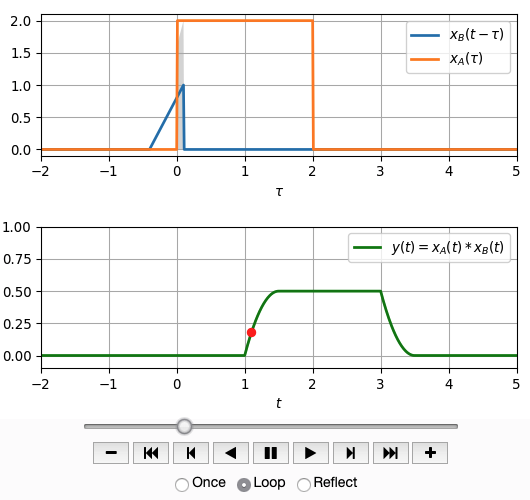
\includegraphics[width=\textwidth]{../convolution_ct/conv_var1_1_1D3D68B312.png}
\caption{Teilüberlappung vorn, also $y_1(t)$.}
\label{fig:1D3D68B312_v1_1}
\end{subfigure}
\begin{subfigure}{0.45\textwidth}
\centering
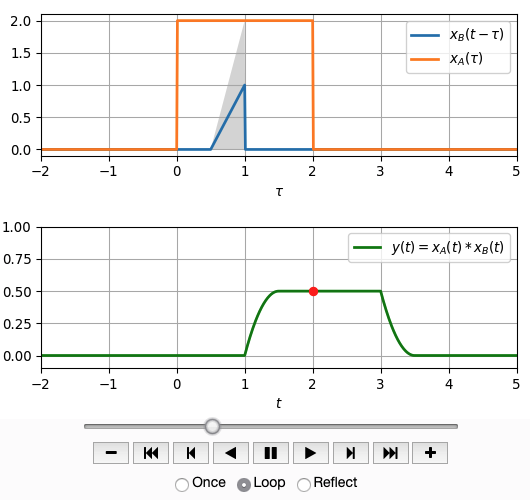
\includegraphics[width=\textwidth]{../convolution_ct/conv_var1_2_1D3D68B312.png}
\caption{Vollständige Überlappung, also $y_2(t)$.}
\label{fig:1D3D68B312_v1_2}
\end{subfigure}
\\
\begin{subfigure}{0.45\textwidth}
\centering
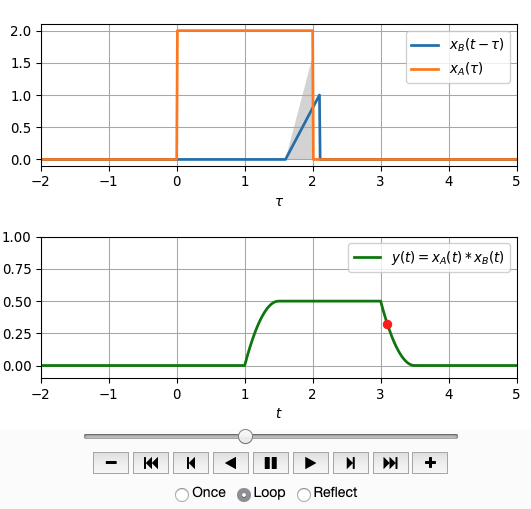
\includegraphics[width=\textwidth]{../convolution_ct/conv_var1_3_1D3D68B312.png}
\caption{Teilüberlappung hinten, also $y_3(t)$.}
\label{fig:1D3D68B312_v1_3}
\end{subfigure}
\begin{subfigure}{0.45\textwidth}
\centering
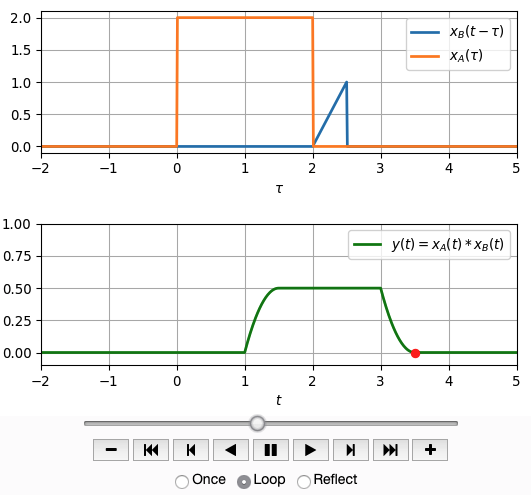
\includegraphics[width=\textwidth]{../convolution_ct/conv_var1_4_1D3D68B312.png}
\caption{Keine Überlappung hinten, also $y_4(t)$.}
\label{fig:1D3D68B312_v1_4}
\end{subfigure}
%
\caption{Faltungsprozess Variante I.
\texttt{convolution\_ct\_example1\_1D3D68B312.ipynb}}
\label{fig:1D3D68B312_v1}
\end{figure*}

\begin{ExCalc}
\textbf{Variante II: Zeitumkehr und Zeitverschiebung}  für $x(t)$
\begin{equation}
y(t) = \int\limits_{-\infty}^{+\infty} x(-\tau+t) h(\tau) \, \fsd \tau
\end{equation}
\begin{itemize}
  \item Schritt 1: Substitution $t\rightarrow \tau$ für $h(t)$
  \begin{equation}
  h(\tau) =
  \begin{cases}
  -2 \tau + 3 \quad \mathrm{für} \quad\red{1} \leq \tau \leq \red{\frac{3}{2}}\\
  0 \quad \mathrm{sonst}
  \end{cases}
  \end{equation}
  \item Schritt 2:  Substitution $t\rightarrow -\tau + t$ für $x(t)$
  \begin{equation}
  x(-\tau+t)=
  \begin{cases}
    2 \quad \mathrm{für} \quad 0 \leq -\tau+t \leq 2\\
    0 \quad \mathrm{sonst}
  \end{cases}
  \end{equation}
  \item Schritt 3:  Intervallgrenzen anpassen
  \begin{equation}
  x(-\tau+t)=
  \begin{cases}
    2 \quad \mathrm{für} \quad \blue{-2+t} \leq \tau \leq \blue{t}\\
    0 \quad \mathrm{sonst}
  \end{cases}
  \end{equation}
  \item Schritt 4: Stammfunktionansatz aufschreiben
  \begin{equation}
  y(t) =
  \int\limits_{a}^{b} x(-\tau+t) \cdot h(\tau) \fsd \tau =
  \int\limits_{a}^{b} 2 \cdot (-2 \tau + 3) \fsd \tau
  \end{equation}
  und berechnen zu
  \begin{equation}
  y(t) = -2 \tau^2 +6 \tau\bigg|_{\tau=a}^{\tau=b}
  \end{equation}
  Die \red{Intervall}\blue{grenzen} gehen als Integrationsbereiche $a,b$ in die Faltung ein.
  \item Schritt 5:  Signal-Überlappungen
  siehe Variante I
  % $x(t)$ ist endliches Signal von $t_1=0$ bis $t_2=2$
  %
  % $h(t)$ ist endliches Signal von $t_3=1$ bis $t_4=\frac{3}{2}$
  %
  % $y(t)$ wird daher ein endliches Signal von $t_1+t_3=1$ bis $t_2+t_4=\frac{7}{2}$ sein
  %
  % es gibt eine Teilüberlappung von $x(\tau)$ und $h(-\tau+t)$  'vorne' von
  % $t_1+t_3$ bis $t_1+t_3+T$
  %
  % es gibt eine Teilüberlappung von $x(\tau)$ und $h(-\tau+t)$  'hinten' von
  % $t_2+t_4-T$ bis $t_2+t_4$
  %
  % $T$ ist die Länge des kürzeren Signals, also hier $T=\frac{1}{2}$
  %
  % vollständige Überlappung hier für von $t = \frac{3}{2}$ bis $t=3$
  %
  % $y(t)=0$ für $t<(t_1+t_3)$ und $t\geq(t_2+t_4)$
  %
  % Diese Erkenntnisse in einer Formel
  % \begin{equation}
  % y(t) =
  % \begin{cases}
  %   y_1(t) \qquad \mathrm{für} \qquad 1 \leq t < \frac{3}{2}\\
  %   y_2(t) \qquad \mathrm{für} \qquad \frac{3}{2} \leq t < 3\\
  %   y_3(t) \qquad \mathrm{für} \qquad 3 \leq t < \frac{7}{2}\\
  %   y_4(t)=0 \qquad \mathrm{sonst}
  % \end{cases}
  % \end{equation}

  \item Schritt 6:  Stammfunktion mit Grenzen auswerten

  \begin{equation}
  y_1(t) = -2 \tau^2 +6 \tau\bigg|_{\tau=\red{1}}^{\tau=\blue{t}}
  = -2 t^2 + 6 t - 4
  \end{equation}

  \begin{equation}
  y_2(t) = -2 \tau^2 +6 \tau\bigg|_{\tau=\red{1}}^{\tau=\red{\frac{3}{2}}}  = \frac{1}{2}
  \end{equation}

  \begin{equation}
  y_3(t) = -2 \tau^2 +6 \tau\bigg|_{\tau=\blue{-2+t}}^{\tau=\red{\frac{3}{2}}} = +2 t^2 - 14 t + \frac{49}{2}
  \end{equation}

\end{itemize}
\end{ExCalc}

\begin{Loesung}
Das Ergebnis der Faltung, also das Ausgangssignal unseres LTI-Systems ist
wie erwartet gleich mit Variante I
\begin{align}
y(t) =
\begin{cases}
  y_1(t) = -2 t^2 + 6 t - 4 &\qquad \mathrm{für} \qquad 1 \leq t < \frac{3}{2}\\
  y_2(t) = \frac{1}{2}  &\qquad \mathrm{für} \qquad \frac{3}{2} \leq t < 3\\
  y_3(t) = +2 t^2 - 14 t + \frac{49}{2} &\qquad \mathrm{für} \qquad 3 \leq t < \frac{7}{2}\\
  y_4(t)=0 &\qquad \mathrm{sonst}
\end{cases}
\end{align}
Im Vergleich zu Variante I ist diese Lösung vielleicht
intuitiver, weil wir die Rechteckfunktion zeitlich verschieben und die
Integrallgrenzen schneller einleuchten.
%
Die Lösung wird in \fig{fig:1D3D68B312_v2} veranschaulicht für verschiedene
Zeiten $t$. In blau der zeitlich umgekehrte, verschobene Rechteckimpuls, in
orange die unverschobene Impulsantwort und in grün das Ausgangssignal der Faltung.
%
Wir sollten uns die \textbf{Unterschiede der Stammfunktionen und der Grenzen in den
Varianten I und II} genau anschauen.
Die Grenzen müssen stimmig sein zu der Funktion die verschoben wird.
%

Einem Rechteckimpuls sieht man nicht durch reines Hinschauen an, dass er
zeitlich gedreht wurde, hier ist also besondere Obacht erforderlich.
%
Gut gemeintes einfaches Integrieren erkaufen wir uns hier also mit tendenzieller
Verwirrung beim Signalspiegeln.
%
Erfahrungsgemäß braucht diese Rechnerei mal einen sehr ruhigen Moment und vertieftes
Sinnieren, während die Faltungsanimation in Dauerschleife läuft, irgendwann
wird klar, was wie verschoben werden muss und mit den Integrationsgrenzen verlinkt
ist.
%
\end{Loesung}















\begin{figure*}[h!]
\centering
\begin{subfigure}{0.45\textwidth}
\centering
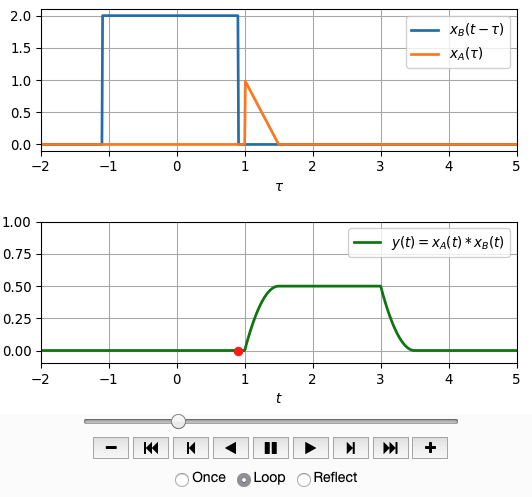
\includegraphics[width=\textwidth]{../convolution_ct/conv_var2_4_1D3D68B312.png}
\caption{Keine Überlappung vorne, also $y_4(t)$.}
\label{fig:1D3D68B312_v2_4}
\end{subfigure}
\begin{subfigure}{0.45\textwidth}
\centering
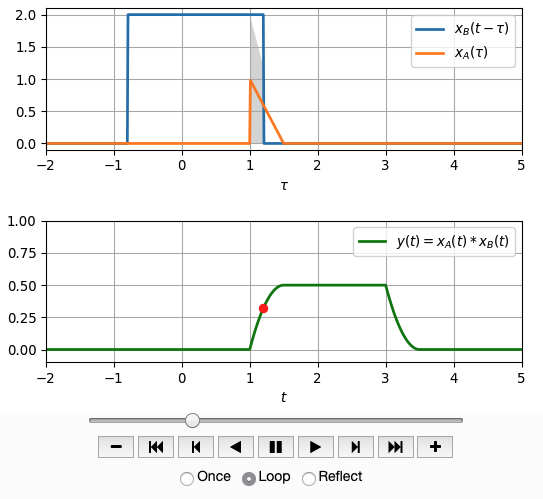
\includegraphics[width=\textwidth]{../convolution_ct/conv_var2_1_1D3D68B312.png}
\caption{Teilüberlappung vorn, also $y_1(t)$.}
\label{fig:1D3D68B312_v2_1}
\end{subfigure}
\\
\begin{subfigure}{0.45\textwidth}
\centering
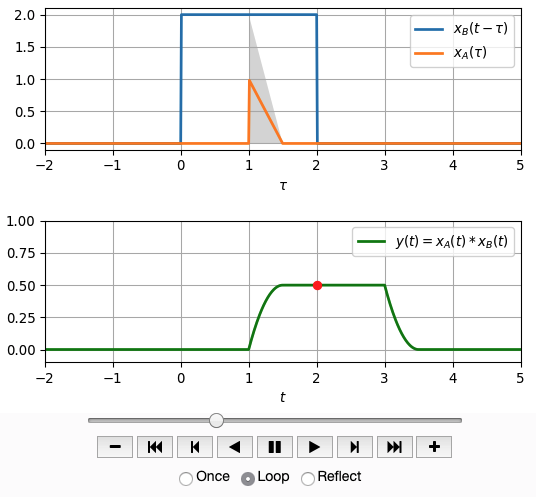
\includegraphics[width=\textwidth]{../convolution_ct/conv_var2_2_1D3D68B312.png}
\caption{Vollständige Überlappung, also $y_2(t)$.}
\label{fig:1D3D68B312_v2_2}
\end{subfigure}
\begin{subfigure}{0.45\textwidth}
\centering
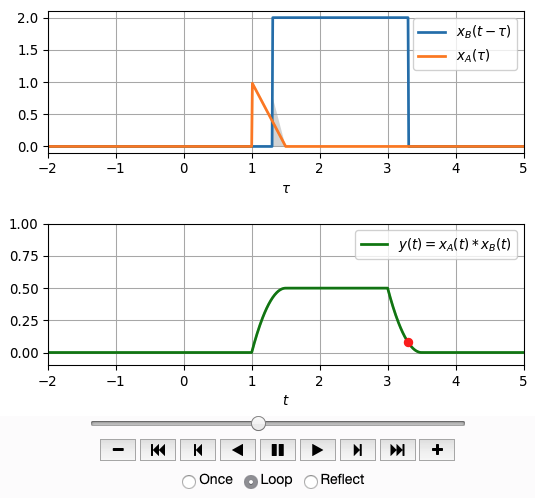
\includegraphics[width=\textwidth]{../convolution_ct/conv_var2_3_1D3D68B312.png}
\caption{Teilüberlappung hinten, also $y_3(t)$.}
\label{fig:1D3D68B312_v2_3}
\end{subfigure}
%
\caption{Faltungsprozess Variante II.
\texttt{convolution\_ct\_example1\_1D3D68B312.ipynb}}
\label{fig:1D3D68B312_v2}
\end{figure*}


\clearpage
\subsection{Faltung Rechteckimpuls mit Exponentialimpuls}
\label{sec:AF3B15E0D3}
\begin{Ziel}
Diese Aufgabe ist sehr ähnlich zu Aufgabe \ref{sec:1D3D68B312}.
Nur die Funktion von $h(t)$ ist verändert, alle Grenzen und
Längenbetrachtungen bleiben jedoch gleich. Das hat einen didaktischen
Hintergrund: Wir wollen hier zu der Erkenntnis kommen, dass eine exp()-Funktion
das Faltungsergebnis an den Sprungstellen anders 'glättet' als der Dreiecksimpuls
vorher.
Wenn wir $h(t)$ wieder als Impulsantwort eines LTI-System auffassen wollen,
heisst das, dass dieses System im Wesen ähnliche Dinge macht, aber im Detail
leicht anderes System-Verhalten hat.
\end{Ziel}
\textbf{Aufgabe} {\tiny AF3B15E0D3}: Berechnen Sie für die in der Skizze dargestellten
endlichen Signale $h(t)$ und $x(t)$ die Faltung $y(t)=x(t) \ast h(t)$.

\begin{tikzpicture}
\begin{axis}[
width=0.5\textwidth,
height=0.3\textwidth,
domain=1:3/2,
samples=20,
legend pos=outer north east,
xlabel = {t / s},
ylabel = {h(t), x(t)},
xmin=-1, xmax=4,
ymin=-0.1, ymax=2.1,
xtick={0,1,1.5,2},
ytick={0,1,2},
ymajorgrids=true,
xmajorgrids=true
]
\addplot[mark=None, color=C1, ultra thick] {exp(-6*(x-1))};
\addplot[mark=None, color=C0, ultra thick]
coordinates {(-1,0)(0,0)(0,2)(2,2)(2,0)(4,0)};
\addplot[mark=None, color=C1, ultra thick]
coordinates {(-1,0)(1,0)(1,1)};
\addplot[mark=None, color=C1, ultra thick]
coordinates {(1.5,0.05)(1.5,0)(4,0)};
\legend{$h(t)=\exp(-[t-1] \cdot 6) \cdot \mathrm{rect}([t-\frac{5}{4}] \cdot 2)$,
$x(t)=2\,\mathrm{rect}([t-1]\cdot \frac{1}{2})$}
\end{axis}
\end{tikzpicture}



\begin{Werkzeug}
Es ist mutmaßlich schöner zu integrieren, wenn wir $x(t)$ zeitlich umkehren und
verschieben, daher
\begin{equation}
y(t) = \int\limits_{-\infty}^{+\infty} x(-\tau+t) h(\tau) \, \fsd \tau
\end{equation}
also analog zur wahrscheinlich zugänglicheren Variante II aus Aufgabe
\ref{sec:1D3D68B312}.
\end{Werkzeug}


\begin{Ansatz}
Signale so darstellen, das wir den stückweisen Verlauf in seinen Grenzen angeben können.
Also: die Exponentialfunktion zeitlich verzögert um 1, schneller abfallend heißt zeitlich
gestaucht, Faktor 6
\begin{equation}
h(t) =
\begin{cases}
\e^{-[t-1]\cdot 6} \quad \mathrm{für} \quad 1 \leq t \leq \frac{3}{2}\\
0 \quad \mathrm{sonst}
\end{cases}
\end{equation}
Und der schon bekannte Rechteckimpuls
\begin{equation}
x(t)=
\begin{cases}
  2 \quad \mathrm{für} \quad 0 \leq t \leq 2\\
  0 \quad \mathrm{sonst}
\end{cases}
\end{equation}
Fassen wir $h(t)$ wieder als Impulsantwort eines LTI-Systems und $x(t)$ als
Eingangssignal in dieses auf. Wir werden gleich sehen, dass wir mit der Denke
sehr nah an der Praxis sind.
\end{Ansatz}




\begin{ExCalc}
Wir benutzen
\textbf{Variante II: Zeitumkehr und Zeitverschiebung}  für $x(t)$
\begin{equation}
y(t) = \int\limits_{-\infty}^{+\infty} x(-\tau+t) h(\tau) \, \fsd \tau
\end{equation}
und folgen unserem Algorithmus:
\begin{itemize}
  \item Schritt 1: Substitution $t\rightarrow \tau$ für $h(t)$
  \begin{equation}
  h(\tau) =
  \begin{cases}
  \e^{-[\tau-1]\cdot 6} \quad \mathrm{für} \quad\red{1} \leq \tau \leq \red{\frac{3}{2}}\\
  0 \quad \mathrm{sonst}
  \end{cases}
  \end{equation}
  \item Schritt 2:  Substitution $t\rightarrow -\tau + t$ für $x(t)$
  \begin{equation}
  x(-\tau+t)=
  \begin{cases}
    2 \quad \mathrm{für} \quad 0 \leq -\tau+t \leq 2\\
    0 \quad \mathrm{sonst}
  \end{cases}
  \end{equation}
  \item Schritt 3:  Intervallgrenzen anpassen
  \begin{equation}
  x(-\tau+t)=
  \begin{cases}
    2 \quad \mathrm{für} \quad \blue{-2+t} \leq \tau \leq \blue{t}\\
    0 \quad \mathrm{sonst}
  \end{cases}
  \end{equation}
  \item Schritt 4: Stammfunktionansatz
  \begin{equation}
  y(t) =
  \int\limits_{a}^{b} x(-\tau+t) \cdot h(\tau) \fsd \tau =
  \int\limits_{a}^{b} 2 \cdot (\e^{-[\tau-1]\cdot 6}) \fsd \tau
  \end{equation}
  und berechnen zu (auch noch ein eher triviales Integral)
  \begin{equation}
  y(t) = -\frac{1}{3}\e^{-[\tau-1]\cdot 6}\bigg|_{\tau=a}^{\tau=b}
  \end{equation}
  Die \red{Intervall}\blue{grenzen} gehen als Integrationsbereiche $a,b$ in die Faltung ein.

  \item Schritt 5:  Signal-Überlappungen

  $x(t)$ ist endliches Signal von $t_1=0$ bis $t_2=2$

  $h(t)$ ist endliches Signal von $t_3=1$ bis $t_4=\frac{3}{2}$

  $y(t)$ wird daher ein endliches Signal von $t_1+t_3=1$ bis $t_2+t_4=\frac{7}{2}$ sein

  es gibt eine Teilüberlappung von $x(\tau)$ und $h(-\tau+t)$  'vorne' von
  $t_1+t_3$ bis $t_1+t_3+T$

  es gibt eine Teilüberlappung von $x(\tau)$ und $h(-\tau+t)$  'hinten' von
  $t_2+t_4-T$ bis $t_2+t_4$

  $T$ ist die Länge des kürzeren Signals, also hier $T=\frac{1}{2}$

  vollständige Überlappung hier für von $t = \frac{3}{2}$ bis $t=3$

  $y(t)=0$ für $t<(t_1+t_3)$ und $t\geq(t_2+t_4)$

  Diese Erkenntnisse in einer Formel
  \begin{equation}
  y(t) =
  \begin{cases}
    y_1(t) \qquad \mathrm{für} \qquad 1 \leq t < \frac{3}{2}\\
    y_2(t) \qquad \mathrm{für} \qquad \frac{3}{2} \leq t < 3\\
    y_3(t) \qquad \mathrm{für} \qquad 3 \leq t < \frac{7}{2}\\
    y_4(t)=0 \qquad \mathrm{sonst}
  \end{cases}
  \end{equation}

  \item Schritt 6:  Stammfunktion mit Grenzen auswerten

  \begin{equation}
  y_1(t) = -\frac{1}{3}\e^{-[\tau-1]\cdot 6}\bigg|_{\tau=\red{1}}^{\tau=\blue{t}}
  = \frac{1}{3}\left(1-\e^{-[t-1] \cdot 6}\right)
  \end{equation}

  \begin{equation}
  y_2(t) = -\frac{1}{3}\e^{-[\tau-1]\cdot 6}\bigg|_{\tau=\red{1}}^{\tau=\red{\frac{3}{2}}}  =
  \frac{1}{3}\left(1-\e^{-3}\right) \approx 0.316737...
  \end{equation}

  \begin{equation}
  y_3(t) = -\frac{1}{3}\e^{-[\tau-1]\cdot 6}\bigg|_{\tau=\blue{-2+t}}^{\tau=\red{\frac{3}{2}}} =
  \frac{1}{3}\left(\e^{-[t-3] \cdot 6} - \e^{-3}\right)
  \end{equation}
\end{itemize}
\end{ExCalc}


\begin{Loesung}
Das gesuchte Faltungsergebnis ist also
\begin{align}
y(t) =
\begin{cases}
  y_1(t) = \frac{1}{3}\left(1-\e^{-[t-1] \cdot 6}\right) &\qquad \mathrm{für} \qquad 1 \leq t < \frac{3}{2}\\
  y_2(t) = \frac{1}{3}\left(1-\e^{-3}\right) \approx 0.316737 &\qquad \mathrm{für} \qquad \frac{3}{2} \leq t < 3\\
  y_3(t) = \frac{1}{3}\left(\e^{-[t-3] \cdot 6} - \e^{-3}\right) &\qquad \mathrm{für} \qquad 3 \leq t < \frac{7}{2}\\
  y_4(t)=0 &\qquad \mathrm{sonst}
\end{cases}
\end{align}

In \fig{fig:AF3B15E0D3_v2} ist der Faltungsprozess veranschaulicht.
%
Stellen wir im Vergleich zu Aufgabe \ref{sec:1D3D68B312} fest, dass
%
\begin{itemize}
  \item die Grenzen für Signalabschnitte gleich geblieben sind (diese Aufgabe war ja so
  ausgelegt)
  \item $y_2(t)$ wieder ein konstanten Verlauf hat, nur diesmal mit der Amplitude von ca.
  $0.316737$. Die Fläche des Exponentialimpulses ist ja kleiner als die des Dreickimpulses
  aus Aufgabe \ref{sec:1D3D68B312}
  \item die Gleichungen, welche die stückweisen Abschnitte definieren diesmal mit der
  Exponentialfunktion beschrieben werden. Auch das sollte wieder einleuchten,
  beim Integrieren einer Exponentialfunktion resultiert wieder eine Exponentialfunktion
\end{itemize}
%
\textbf{Ladekurven Kondensator?!?} Wenn wir uns das Faltungsergebnis $y(t)$
(grüner Graph) und die Ergebnisgleichungen anschauen, wird uns
vielleicht eine verblüffende Ähnlichkeit zu Auf-/Entladekurven eines
RC-Gliedes auffallen. Wir schauen uns das in der nächsten Aufgabe \ref{sec:C964DD7400}
genauer an. Hier schon mal soviel, es ist sehr ähnlich aber nicht exakt identisch.
Der Grund liegt in der hier betrachteten \textbf{endlichen} Impulsantwort. Ein
RC-Glied hat eine \textbf{unendliche} Impulsantwort.
\end{Loesung}


\begin{figure*}[h!]
\centering
\begin{subfigure}{0.45\textwidth}
\centering
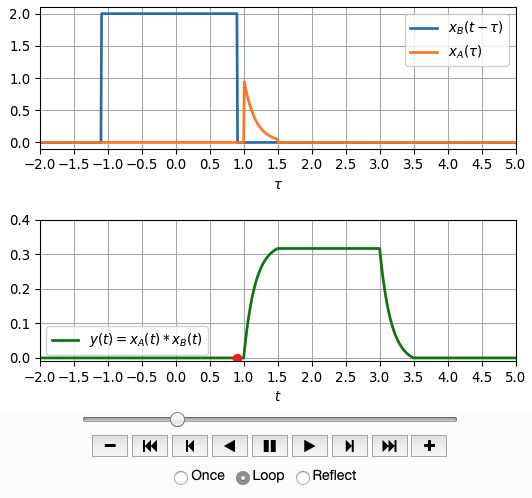
\includegraphics[width=\textwidth]{../convolution_ct/conv_var2_4_AF3B15E0D3.png}
\caption{Keine Überlappung vorne, also $y_4(t)$.}
\label{fig:AF3B15E0D3_v2_4}
\end{subfigure}
\begin{subfigure}{0.45\textwidth}
\centering
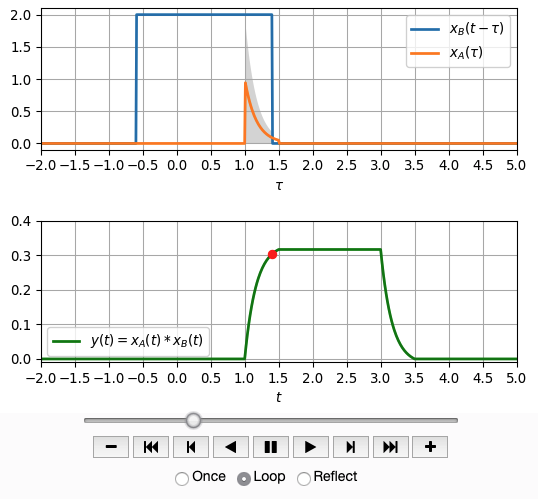
\includegraphics[width=\textwidth]{../convolution_ct/conv_var2_1_AF3B15E0D3.png}
\caption{Teilüberlappung vorn, also $y_1(t)$.}
\label{fig:AF3B15E0D3_v2_1}
\end{subfigure}
\\
\begin{subfigure}{0.45\textwidth}
\centering
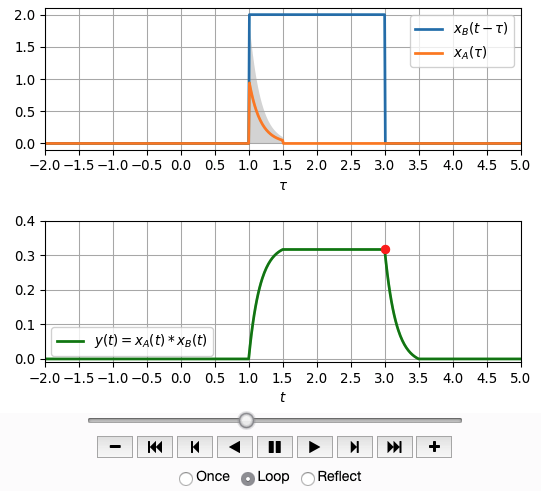
\includegraphics[width=\textwidth]{../convolution_ct/conv_var2_2_AF3B15E0D3.png}
\caption{Vollständige Überlappung, also $y_2(t)$.}
\label{fig:AF3B15E0D3_v2_2}
\end{subfigure}
\begin{subfigure}{0.45\textwidth}
\centering
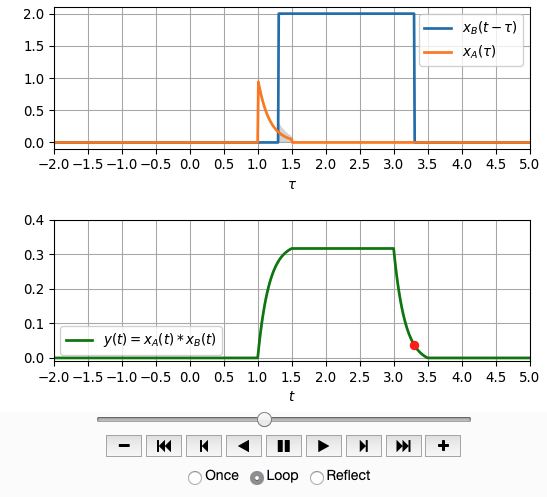
\includegraphics[width=\textwidth]{../convolution_ct/conv_var2_3_AF3B15E0D3.png}
\caption{Teilüberlappung hinten, also $y_3(t)$.}
\label{fig:AF3B15E0D3_v2_3}
\end{subfigure}
%
\caption{Faltungsprozess Aufgabe \ref{sec:AF3B15E0D3}.
\texttt{convolution\_ct\_example2\_AF3B15E0D3.ipynb}}
\label{fig:AF3B15E0D3_v2}
\end{figure*}



\clearpage
\subsection{Faltung Rechteckimpuls mit Exponentialfunktion}
\label{sec:C964DD7400}
\begin{Ziel}
Wir werden anhand einer speziellen Faltung eines endlichen Signals mit
einem unendlichen Signal, einen ganz fundamentalen Link zur Elektrotechnik
und DGLs 1. Ordnung mit konstanten Koeffizienten herstellen:
Sprungartige Spannungsänderungen an passiven Energiespeichern (Auf-/Entladen) können wir
sehr elegant mit Signal-und Systemtheorie Werkzeugen berechnen. Es wird mit
der Laplace Transformation später sogar noch eleganter.
\end{Ziel}
\textbf{Aufgabe} {\tiny C964DD7400}: Für das unten abgebildete RC-Glied
(Annahme: ideale Bauelemente)
gilt die \textbf{Impulsantwort} (wir nehmen LTI System-Eigenschaften an)
\begin{equation}
h(t) = \frac{1}{T_\mathrm{RC}} \cdot \e^{-\frac{t}{T_\mathrm{RC}}}
\qquad \mathrm{für} \qquad t \geq 0
\qquad \mathrm{mit} \qquad T_\mathrm{RC} = R \cdot C
\end{equation}
Wir betrachten das RC-Glied als ruhend, also $y(0)=0$.
%
Berechnen Sie für $T_\mathrm{RC}=\frac{1}{5}$ s und für das unten dargestellte
Eingangssignal $x(t)$ das Faltungsergebnis $y(t)=x(t) \ast h(t)$.
%
\begin{center}
\begin{circuitikz}[european, scale=0.75]
\node (in) at (1,0){};
\node (in_ground) at (1,-3){};
\node (out) at (4,0){};
\node (out_ground) at (4,-3){};
\draw (in) to [R,l_=$R$,o-] (3,0);
\draw (3,0) to [short,-o,] (out);
\draw (3,0) to [C,l_=$C$,*-*] (3,-3);
\draw (in_ground) to [short,o-o] (out_ground);
\path[draw, bend right, ->, >=latex] (in) edge node[left]{Eingangsspannung $x(t)$} (in_ground);
\path[draw, bend left, ->, >=latex] (out) edge node[right]{Ausgangsspannung $y(t)$} (out_ground);
\end{circuitikz}
\end{center}
%
\begin{tikzpicture}
\begin{axis}[
width=0.5\textwidth,
height=0.3\textwidth,
domain=0:4,
samples=50,
legend pos=outer north east,
xlabel = {t / s},
ylabel = {h(t), x(t)},
xmin=-1, xmax=4,
ymin=-0.1, ymax=1.1,
xtick={0,1,2,3},
ytick={0,0.5,1,1.5,2},
ymajorgrids=true,
xmajorgrids=true
]
\addplot[mark=None, color=C0, ultra thick]
coordinates {(-1,0)(0,0)(0,1)(2,1)(2,0)(4,0)};
\addplot[mark=None, color=C1, ultra thick]
coordinates {(-1,0)(0,0)(0,1)};
\addplot[mark=None, color=C1, ultra thick] {exp(-5*(x))};
\legend{$x(t)=\mathrm{rect}([t-1]\cdot \frac{1}{2})$,
$\frac{1}{5} \cdot h(t)=\exp(- t \cdot 5) \cdot \epsilon(t)$}
\end{axis}
\end{tikzpicture}

\noindent\textbf{Hinweis 1}: Wir werden nach der Übung~\ref{sec:ue3_laplace} (3) in der Lage sein, $h(t)$ elegant herzuleiten.
Nehmen wir das an dieser Stelle mal hin, aber bemerken auch, dass wir
diese Art Formel beim Kondensator eh schon mal gesehen haben, mutmaßlich aber
nicht im Kontext einer Impulsantwort.

\noindent\textbf{Hinweis 2}: In der Elektrotechnik verwenden wir gerne $\tau$ für die Zeitkonstante. Weil das
aber unsere Hilfsvariable in der Faltung ist, geben wir der Zeitkonstante des RC-Glieds die Variable
$T_\mathrm{RC}$.

\noindent\textbf{Hinweis 3}: Aufgabe \ref{sec:AF3B15E0D3} behandelte den \textbf{endlichen Exponentialimpuls}
mit einer Zeitkonstante $1/6$ s, hier verwenden wir die abfallende Exponentialfunktion
die sich nur asymptotisch gegen Null nähert, die also eine \textbf{unendliche Impulsantwort}
darstellt. Der schöneren Anschauung wegen, wählen wir $T_\mathrm{RC}=1/5$ s, weil
dann bei 1 s zu 99\% der finale Lade-/Entlade-Amplitudenwert erreicht ist
(vgl. $5 T_\mathrm{RC}$-Regel).

\noindent\textbf{Hinweis 4}: Machen wir uns noch klar, dass wir es hier mit der DGL 1. Ordnung
mit konstanten Koeffizienten
\begin{equation}
T_\mathrm{RC} \frac{\fsd y(t)}{\fsd t} + y(t) = x(t)
\end{equation}
mit $y(0)=0$ zu tun haben und überlegen, wie wir die Aufgabe mit
typischem Mathe-DGL Handwerk lösen würden. Siehe auch SigSys-Klausur WS19/20 Aufgabe 1.

\begin{Werkzeug}
Es ist mutmaßlich wieder schöner zu integrieren,
wenn wir $x(t)$ zeitlich umkehren und verschieben, daher Faltungsintegral
\begin{equation}
y(t) = \int\limits_{-\infty}^{+\infty} x(-\tau+t) h(\tau) \, \fsd \tau
\end{equation}

\end{Werkzeug}
\begin{Ansatz}
Die Signale zum Falten sind
\begin{equation}
h(t) =
\begin{cases}
\frac{1}{\frac{1}{5}} \e^{-\frac{t}{\frac{1}{5}}} = 5 \e^{-5 t} \quad \mathrm{für} t \geq 0\\
0 \quad \mathrm{sonst}
\end{cases}
\end{equation}
\begin{equation}
x(t)=
\begin{cases}
  1 \quad \mathrm{für} \quad 0 \leq t \leq 2\\
  0 \quad \mathrm{sonst}
\end{cases}
\end{equation}
\end{Ansatz}

\begin{ExCalc}
Wir benutzen
\textbf{Variante II: Zeitumkehr und Zeitverschiebung}  für $x(t)$
\begin{equation}
y(t) = \int\limits_{-\infty}^{+\infty} x(-\tau+t) h(\tau) \, \fsd \tau
\end{equation}
Wir können diesmal nicht unseren bereits etablierten Algorithmus verwenden, weil
der nur funktioniert, wenn beide Signale endliche Länge haben.
%
Machen wir uns hier stattdessen zu nutze, dass die Rechteckfunktion durch zwei
Sprungfunktionen dargestellt werden kann, nämlich $x(t) = \epsilon(t) - \epsilon(t-2)$.
%
Es gilt das Superpositionsprinzip bei LTI-Systemen. Daher
können wir für die beiden einzelnen Sprünge die Faltungen einzeln ausrechnen.
%
Das gelingt besonders elegant, wenn man für die Faltung die Sprünge als die
zeitumgekehrten und verschobenen Signale auffasst (damit wäre Klausuraufgabe 1
vom SS2019 ganz schnell berechnet).
%
Konkret also: Faltung mit der Sprungfunktion $x_1(t) = \epsilon(t)$ führt auf
\begin{equation}
y_1(t) = \int\limits_{0}^{t} 1 \cdot 5 \e^{- 5 \tau} \fsd \tau= \left(1-\e^{-5 t}\right)
\qquad \mathrm{für} \qquad t \geq 0
\end{equation}
%
Faltung mit der Sprungfunktion $x_2(t) = -\epsilon(t-2)$ führt auf
\begin{equation}
y_2(t) =
\begin{cases}
  0 &\qquad \mathrm{für} \qquad t < 2\\
  \int\limits_{2}^{t} -1 \cdot 5 \e^{- 5 [\tau-2]}  \fsd \tau = \left( \e^{-5 [t-2]}-1\right) &\qquad \mathrm{für} \qquad t \geq 2
\end{cases}
\end{equation}
%
% Bitte nochmal mit Wolfram Alpha gegenchecken:
% Ansatz für gedrehte Impulsantwort
% integrate -step(tau-2)*5*exp(5*tau-5*t) d tau from 0 to t
% oder Ansatz für gedrehten Reckteckimpuls
% integrate -step(-tau+t-2)*5*exp(-5*tau) d tau from 0 to t

% Mit dem zweiteren, hab ich dann für 2.217 die beiden Funktionen verschoben (bzgl. tau) und die Integralgrenzen angepasst
% integrate -step(-tau+t)*5*exp(-5*(tau-2)) d tau from 2 to t
% und wenn wir dann explizit erwähnen, dass y(t) nur für t>=2, brauchen wir die step funktion im Integral nicht mehr und wir können mit dem Integral
% integrate -5*exp(-5*(tau-2)) d tau from 2 to t
% rechnen.
% %
% Es gilt das Superpositionsprinzip bei LTI-Systemen, also einer Eingangssumme
% $x(t) = x_1(t) + x_2(t) = \epsilon(t) - \epsilon(t-2)$
% folgt die Ausgangssumme $y(t) = y_1(t) + y_2(t)$.
\end{ExCalc}

\begin{Loesung}
Das Endergebnis lautet mit Superposition
\begin{equation}
y(t) = y_1(t) + y_2(t) =
  \begin{cases}
  \left(1-\e^{-5 t}\right) &\qquad \mathrm{für} \qquad 0 \leq t < 2\\
  \left(1-\e^{-5 t}\right) + \left( \e^{-5 [t-2]}-1\right) = \e^{-5 [t-2]} - \e^{-5 t}
  &\qquad \mathrm{für} \qquad t \geq 2
  \end{cases}
\end{equation}
und wir erkennen im ersten Teil der Gleichung die typische Aufladekurve des
Kondensators. Im zweiten Teil ist die nicht ganz so offensichtliche Entladekurve
zu sehen, wir entladen erst zum Zeitpunkt $t=2$ s, das muss in der exp()-Funktion
als Zeitverschiebung mit berücksichtigt werden.
%
Die gewählte Zeitkonstante ist sehr kurz im Vergleich zum Rechtecklänge, daher
kann man für den Kondensator mit guter Näherung drei Zustände während des
Anlegens von $x(t)$ definieren:
\begin{itemize}
  \item für $0<t<1$ Aufladen
  \item für $1<t<2$ Geladen
  \item für $2<t<3$ Entladen
\end{itemize}
Wie oben schon erwähnt, erfolgt vollständiges Aufladen und Entladen mit asymptotischer
Annäherung an den Endzustand.

Spannende Frage zum Sinnieren oder vielleicht sogar Rechnen:
Wie schaut das Ausgangssignal $y(t)$ aus, wenn man den Rechtecksprung sehr,
sehr, sehr kurz macht und vielleicht sogar Fläche 1 sicherstellt?

Spannender Link I: Wir haben mit
\begin{align}
y_1(t) =
\begin{cases}
1-\e^{-5 t} \quad \text{für} \quad t\geq 0\\
0 \quad \text{sonst}
\end{cases}
\end{align}
die sogenannte \textbf{Sprungantwort} $h_\epsilon(t)$ des Systems berechnet,
sozusagen als Abfallprodukt, weil wir die Sprungfunktion als Systemeingang gewählt
haben, und das System eben antwortet mit der ... Sprungantwort.

Spannender Link II: Die \textbf{Impulsantwort} $h(t)$ ist direkt proportional zur
Entladekurve eines Kondensators, wenn der Kondensator zum Zeitpunkt $t=0$
vollständig auf $U_q$ aufgeladen war und ab $t=0+$ die Entladung erfolgt.
Aus der Elektrotechnik wissen wir, dass dann $y(t) = U_q \e^{-\tau/T_\mathrm{RC}}$ gilt,
wir sehen Ähnlichkeiten mit $h(t) = \frac{1}{T_\mathrm{RC}} \cdot \e^{-\frac{t}{T_\mathrm{RC}}}$...

Wir bekommen langsam ein Gespür für die größeren Zusammenhänge und
warum SigSys nützlich sein könnte.
\end{Loesung}


\begin{figure*}[h!]
\centering
\begin{subfigure}{0.45\textwidth}
\centering
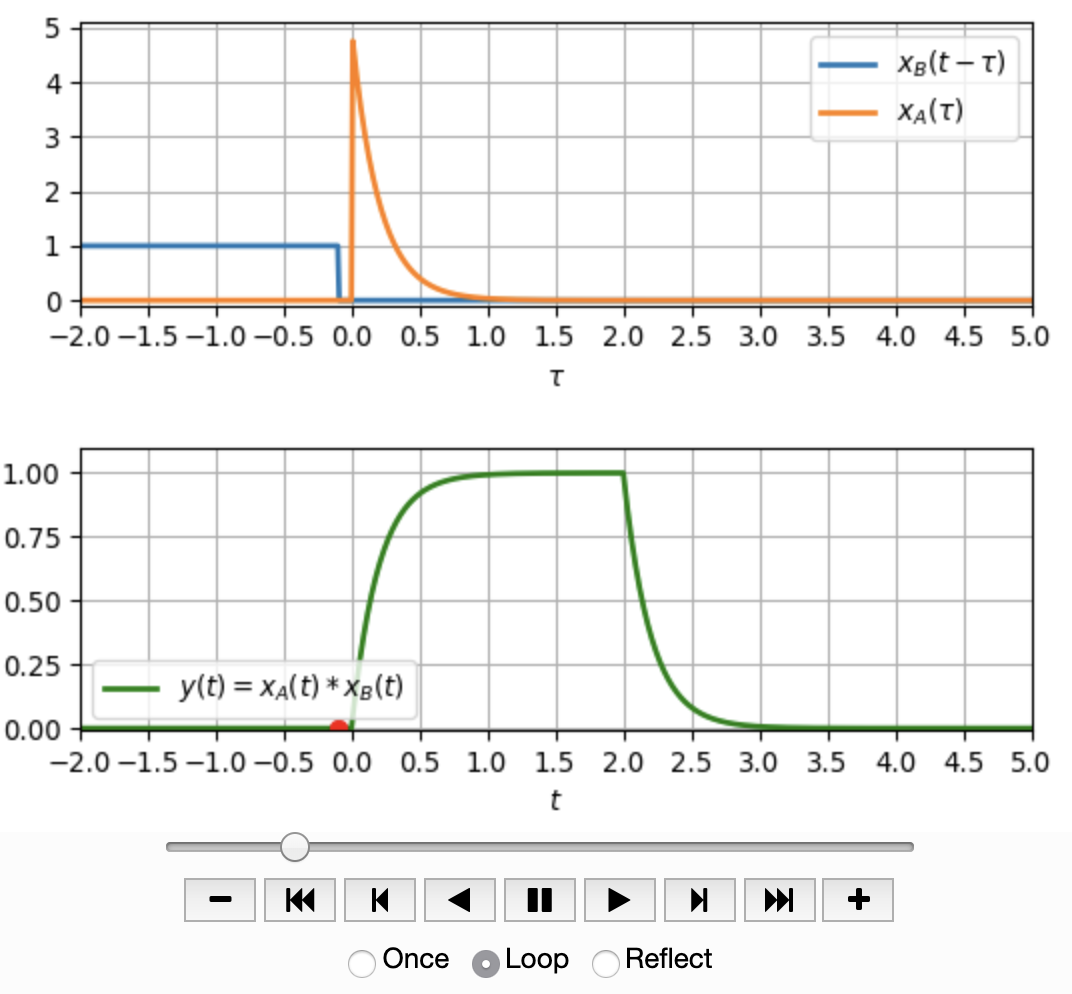
\includegraphics[width=\textwidth]{../convolution_ct/conv_var2_1_C964DD7400.png}
\caption{Keine Überlappung vorne.}
\label{fig:C964DD7400_v2_1}
\end{subfigure}
\begin{subfigure}{0.45\textwidth}
\centering
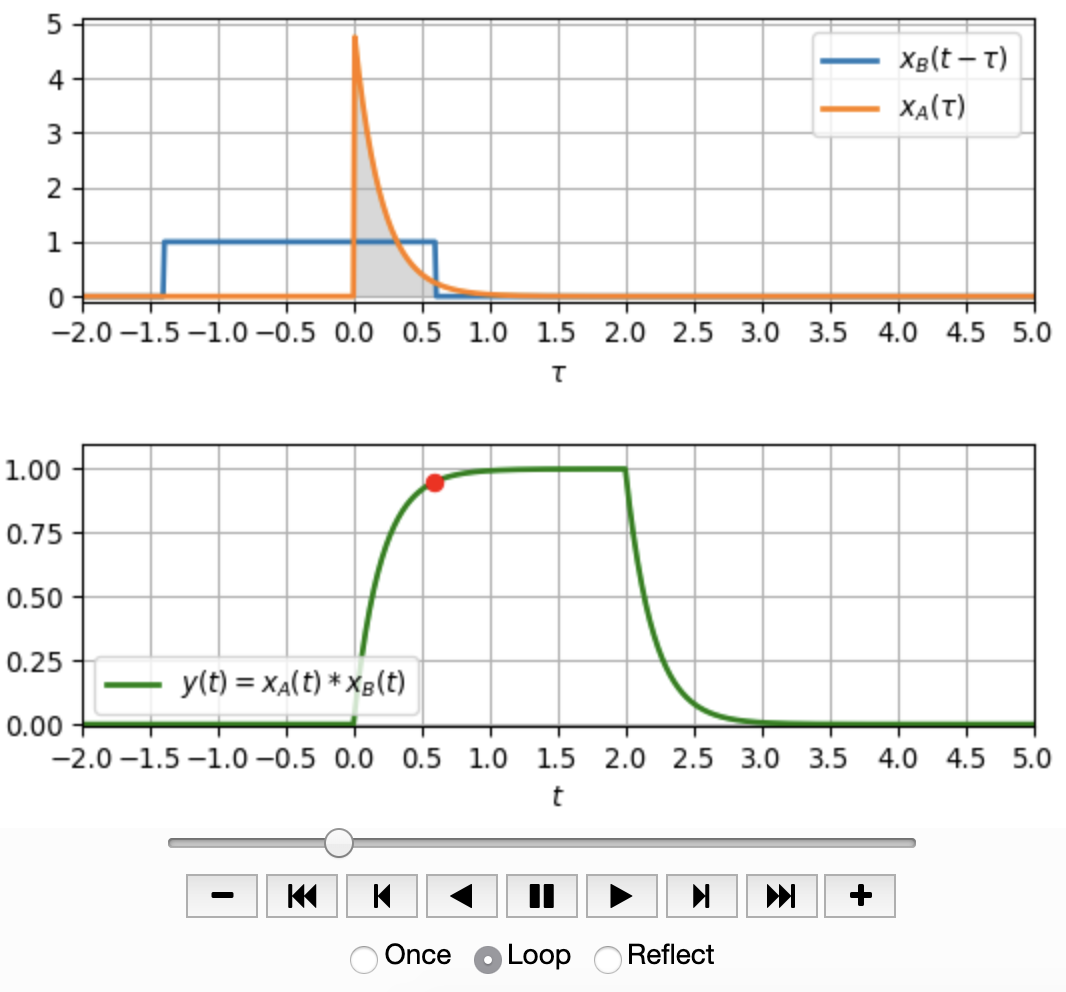
\includegraphics[width=\textwidth]{../convolution_ct/conv_var2_2_C964DD7400.png}
\caption{Teilüberlappung, Ladezustand: 95\%.}
\label{fig:C964DD7400_v2_2}
\end{subfigure}
\\
\begin{subfigure}{0.45\textwidth}
\centering
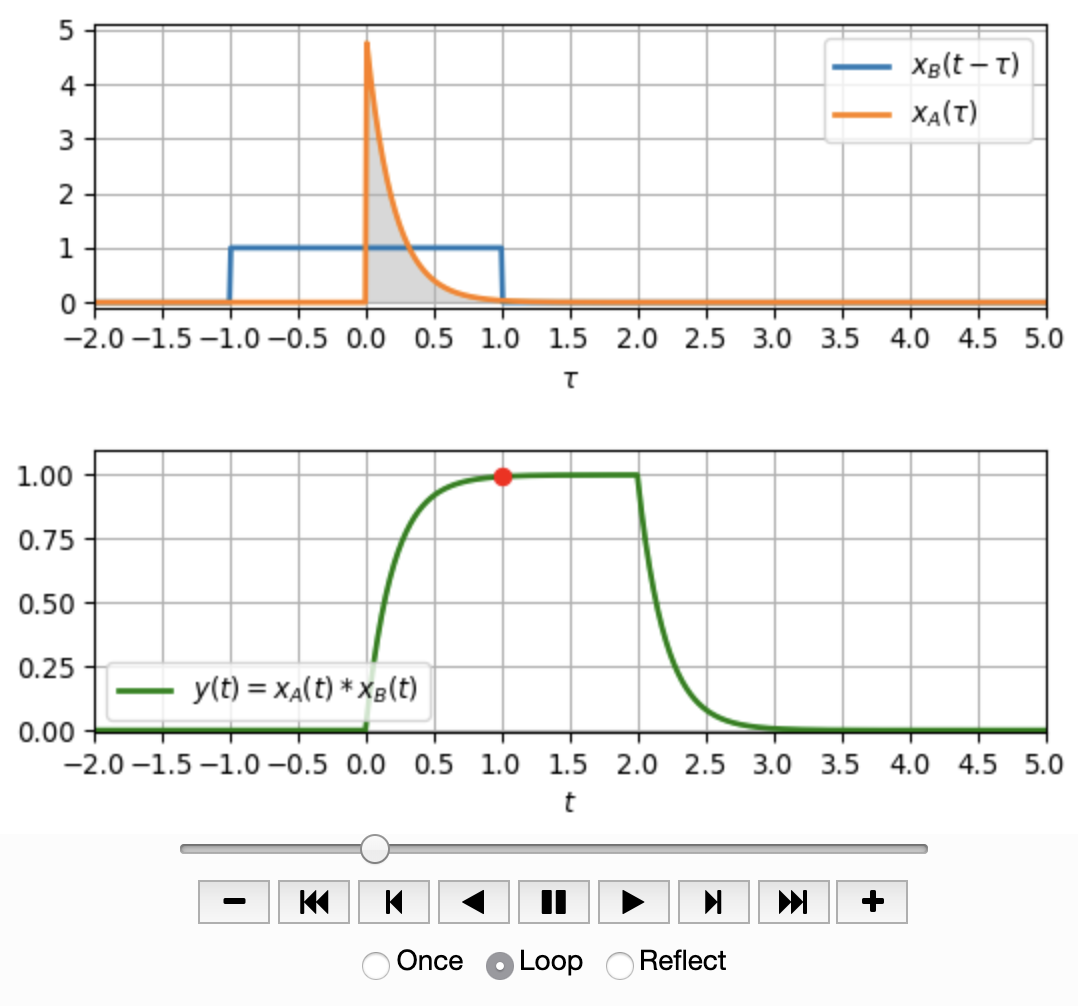
\includegraphics[width=\textwidth]{../convolution_ct/conv_var2_3_C964DD7400.png}
\caption{Teilüberlappung, Ladezustand: 99\%.}
\label{fig:C964DD7400_v2_3}
\end{subfigure}
\begin{subfigure}{0.45\textwidth}
\centering
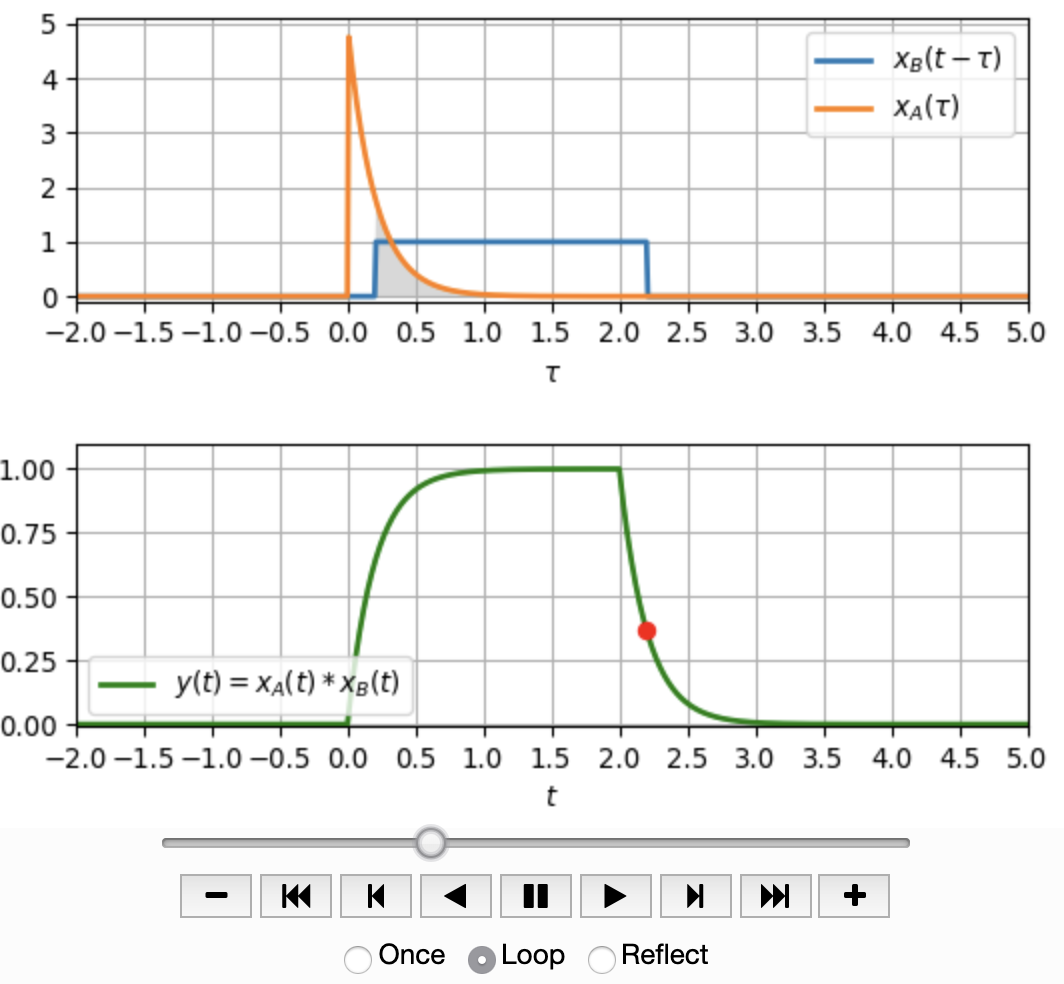
\includegraphics[width=\textwidth]{../convolution_ct/conv_var2_4_C964DD7400.png}
\caption{Teilüberlappung, Ladezustand: 37\% .}
\label{fig:C964DD7400_v2_4}
\end{subfigure}
%
\caption{Faltungsprozess Aufgabe \ref{sec:C964DD7400}.
\texttt{convolution\_ct\_example3\_C964DD7400.ipynb}}
\label{fig:C964DD7400_v2}
\end{figure*}

\newpage
Wolfram Alpha löst einfache Faltungen analytisch und plotted die Signalverläufe
des Ergebnissignals. Folgende Beispiele mit immer
dem gleichen Rechtecksignal, aber unterschiedlichen Impulsantworten

\verb| Convolve[rect(1/4*(t-2)), 2*exp(-t/(1/2))*Step(t)]|

\verb| Convolve[rect(1/4*(t-2)), tri(t)*Step(t)]|

\verb| Convolve[rect(1/4*(t-2)), tri(t-1) * rect((t-1/2))]|

\verb| Convolve[rect(1/4*(t-2)), rect(t-1/2)]|

verdeutlichen nochmal schön die unterschiedlichen Auflade- und Entlade-Vorgänge
bedingt durch unterschiedliche Impulsantwortfunktionen. Wenn wir diese Verläufe
durch Überlegung schematisch herleiten können, haben wir im Grunde das Wesen der
Faltung verstanden.
  % UE 2, signal ops, LTI, conv

%------------------------------------------------------------------------------

\setcounter{section}{2}
%%------------------------------------------------------------------------------
\clearpage
\section{UE 3: Laplace Transformation}
\label{sec:ue3_laplace}
%
Wir haben Laplace Transformation sicherlich schon in einer Mathe Vorlesung
kennengelernt.
Laplace Transformation ist eine Integraltransformation aus der Familie
\begin{equation}
F(y) = \int\limits_{x_1}^{x_2} f(x) \cdot K(x,y) \fsd x
\end{equation}
mit dem Integralkern $K(x,y) = \e^{-x\,y}$.
Wir verwenden in SigSys vorwiegend für die Variable $x$ die Zeit $t$ und für
$y$ die Laplace/Bild Variable $s\in\mathbb{C}$ (in älterer Literatur finden
wir auch oft die Variable $p$, wahrscheinlich um den Link zur Namensgebung
La\underline{p}lace zu machen).
Als Grenzen benutzen wir oft $x_1=0$ und $x_2=\infty$ um kausale Signale und
Systeme beschreiben zu können.
%
Die Rücktransformation ist wegen $s\in\mathbb{C}$ ein komplexes Wegintegral.

Wir verwenden Signal-Transformationen, in der Hoffnung, dass a) Probleme im
transformierten Signalraum, dem sogenannten Bildbereich einfacher zu lösen
sind als im Originalbereich und b) dass Signale einfacher/kompakter darstellbar
sind (vgl. periodisches Signal vs. Koeffizienten der Fourierreihe).
%
Die Wahl der geeignetsten Transformation ist dabei entscheidend, weil eine
ungeeignete das Problem auch komplizierter machen kann.
%
Die Laplace Transformation ist nun deswegen herausragend geeignet, weil
wir Signale \textbf{und} LTI-Systeme analysieren \textbf{und} synthetisieren
können und deswegen Signale mit Systemen elegant und konsistent verknüpfen können.

Wir sollten uns klarmachen, dass der \textbf{Wunsch nach einem einfacherem Operator
für die zeitliche Ableitung} ein Ausgangspunkt für die Erfindung der Laplace
Transformation ist; das sehr lesenswerte, zeitlose Lehrwerk \cite{LangeSigSys1} enthält
einen Abschnitt über die Entwicklungshistorie bis in die 1970er.
Statt Ableiten, also Multiplizieren
\begin{equation}
  \frac{\fsd }{\fsd t} (\cdot) \rightarrow s(\cdot ) \text{ mit } s \in \mathbb{C}
\end{equation}
unter Beibehaltung der Skalierungseigenschaft (Multiplikation mit Konstanten)
und Additionseigenschaft (Superposition).
%
Viele Mathematiker*innen haben sich an dieser Fragestellung der Operatorentheorie
abgearbeitet, sie ist ja zunächst aus rein mathematischer hochspannend, und
es hat sich herausgestellt, dass ein Spezialfall
(nämlich für $y=s\in\mathbb{C}$\footnote{die Integraltransformation mit $y=\im\omega$
, also $y$ rein imaginär, erfüllt unsere Anforderung an den neuen Operator nicht ganz,
weil eben der für bestimmte Betrachtungen wichtige Realteil in $y$ fehlt.
Wir werden sie aber trotzdem sehr nützlich finden
für SigSys, es ist die Fouriertransformation.})
der obigen
Integraltransformation genau das gewünschte leistet. Es wurde definiert
\begin{align}
\mathcal{L}\{x(t)\} = \int\limits_{t=0}^{\infty} x(t) \cdot \e^{-s\,t} \fsd t,
\end{align}
später deklariert als einseitige Laplace Transformation, benutzbar
für kausale Signale.
%
Die Laplace Transformation ist ein linearer Operator, d.h.
es gilt Additionseigenschaft
\begin{align}
\mathcal{L}\{x_1(t)+x_2(t)\} = \mathcal{L}\{x_1(t)\} + \mathcal{L}\{x_2(t)\}
\end{align}
und die Skalierungseigenschaft
\begin{align}
\mathcal{L}\{a x(t)\} = a \mathcal{L}\{x(t)\}.
\end{align}

Schauen wir uns kurz an, wie der Wunsch nach
$\frac{\fsd }{\fsd t} (\cdot) \rightarrow s(\cdot )$
mittels der Integraltransformation erfüllt wird, also was passiert mit
\begin{align}
\mathcal{L}\{\frac{\fsd }{\fsd t}  x(t)\} &= \int\limits_{t=0}^{\infty} \frac{\fsd }{\fsd t}  x(t) \cdot \e^{-s\,t} \fsd t
\end{align}
Die partielle Integration hilft dies anders darzustellen
\begin{align}
&\int u v' \fsd t + \int v u' \fsd t = u\,v\\
&\int u v' \fsd t = u\,v - \int v u' \fsd t\\
&u = \e^{-s\,t}\qquad u' = -s\,\e^{-s\,t}\\
&v = x(t)\qquad v' = \frac{\fsd }{\fsd t}  x(t)\\
&\int\limits_{t=0}^{\infty} \e^{-s\,t} \frac{\fsd }{\fsd t}  x(t) \, \fsd t
= \e^{-s\,t}\,x(t)\bigg|_{t=0}^{\infty} - \int\limits_{t=0}^{\infty} x(t) \cdot (-s\,\e^{-s\,t}) \, \fsd t\\
&\int\limits_{t=0}^{\infty} \e^{-s\,t} \frac{\fsd }{\fsd t}  x(t) \, \fsd t
= s \cdot \int\limits_{t=0}^{\infty} x(t) \e^{-s\,t} \, \fsd t
+\e^{-s\,t}\,x(t)\bigg|_{t=0}^{\infty}\\
&\int\limits_{t=0}^{\infty} \e^{-s\,t} \frac{\fsd }{\fsd t}  x(t) \, \fsd t
= s \cdot \int\limits_{t=0}^{\infty} x(t) \e^{-s\,t} \, \fsd t - x(0)
\end{align}
und wir stellen fest, dass
\begin{align}
\mathcal{L}\{\frac{\fsd }{\fsd t}  x(t)\}  = s \cdot \mathcal{L}\{x(t)\} - x(0)
\end{align}
also tatsächlich die lineare Operation \textbf{zeitliche Ableitung} zur Operation
\textbf{Multiplikation mit} $s$ gemacht wurde. Dabei müssen wir zusätzlich den
\textbf{Anfangswert} $x(0)$ beachten.

Wie bildet sich nun der Umkehroperator der zeitlichen Ableitung, also die zeitliche
Integration ab? Es gilt
\begin{align}
\mathcal{L}\{\int\limits_{0}^{t} x(\tau)\fsd \tau\}  = \frac{1}{s} \cdot \mathcal{L}\{x(t)\}.
\end{align}
Damit haben wir zwei ganz wichtige Operatoreigenschaften für
$x(t)\quad\laplace\quad X(s)$ zusammengetragen:
\begin{align}
\text{Differentiation:   } &\frac{\fsd }{\fsd t}  x(t) \quad\laplace\quad s\cdot X(s) - x(0)\\
\text{Integration:   } &\int\limits_{0}^{t} x(t) \quad\laplace\quad \frac{1}{s} \cdot X(s)
\end{align}
%
Weitere fundamentale Eigenschaften, die wie oft benötigen sind
\begin{align}
\text{Zeitverschiebung:   } x(t-\tau)& \quad\laplace\quad \e^{-s\,\tau} X(s)\\
\text{Bildbereichsverschiebung:   } \e^{a\,t} \, x(t)& \quad\laplace\quad X(s-a)
\end{align}
Die Bildbereichsverschiebung ist auch als Modulationstheorem bekannt,
und wir werden es in den Aufgaben dieser Übung ausführlich kennenlernen und
benutzen.


Die eigentliche Essenz der Laplace Transformation für die Anwendung in
SigSys steckt in der Eigenschaft
\begin{align}
\label{eq:laplace_intro_ast_mult}
x(t) \ast h(t) \quad\laplace\quad X(s) \cdot H(s),
\end{align}
d.h. das 'Abfallprodukt' für die Einführung eines einfacheren Operators
für die zeitliche Ableitung ist, dass die Faltung im Zeitbereich durch die
Multiplikation im Bildbereich dargestellt wird. Das dürfen wir durchaus fancy finden, ist aber
kein Zufall.

Die mathematisch saubere Verortung des Dirac Impulses war im Erfindungsprozess
der Laplace Transformation nicht einfach. Nachdem wir uns für SigSys mit Einführung
der Definition (zur Erinnerung: kein klassisches Riemann-Integral!)
\begin{equation}
\int\limits_{-\infty}^{+\infty} \delta(t-\tau) \cdot f(t) \, \fsd t \stackrel{\mathrm{def}}= f(\tau)
\end{equation}
eine nützliches, einfaches Werkzeug gebastelt haben, sollten wir das auch
benutzen.
Wir nehmen $\tau=0$
\begin{equation}
\int\limits_{-\infty}^{+\infty} \delta(t) \cdot f(t) \, \fsd t \stackrel{\mathrm{def}}= f(0)
\end{equation}
und für den Integralkern der Laplace Transformation $f(t)=\e^{-s \cdot t}$
ergibt sich
\begin{equation}
\int\limits_{-\infty}^{+\infty} \delta(t) \cdot \e^{-s \cdot t} \, \fsd t \stackrel{\mathrm{def}}= \e^{-s \cdot 0} = 1
\end{equation}
bzw. nochmal in Operatorschreibweise, weil fundamental wichtig:
%
\begin{equation}
  \mathcal{L}\{\delta(t)\} = 1
  \text{ oder anders notiert }
  \delta(t) \quad\laplace\quad 1.
\end{equation}
%
Der Dirac Impuls bildet also die gesamte komplexe $s$-Ebene gleich gewichtet ab.
%
Wir werden in den Aufgaben sehen, dass für den Einheitssprung
\begin{equation}
  \mathcal{L}\{\epsilon(t)\} = \frac{1}{s}
  \text{ oder anders notiert }
  \epsilon(t) \quad\laplace\quad \frac{1}{s}
\end{equation}
gilt.
Die Integrationsregel der Laplace Transformation liefert uns hier sehr bequem
den einfachen Zusammenhang
\begin{equation}
  \int\limits_{0}^{t} \delta(\tau)\fsd \tau = \epsilon(t),
\end{equation}
mit dem wir uns wegen der Signalunstetigkeiten immer ein wenig schwer tun.
%
Wenn wir $x(t)=\delta(t)$ in \eq{eq:laplace_intro_ast_mult} einsetzen
\begin{align}
\delta(t) \ast h(t) \quad\laplace\quad 1 \cdot H(s)
\end{align}
und beachten, dass der Dirac Impuls das Neutralelement der Faltung ist,
also $h(t) = \delta(t) \ast h(t)$ bekommen wir
\begin{align}
h(t) \quad\laplace\quad H(s).
\end{align}
Anders herum gedacht, die Faltung eines Signals mit einem Dirac Impuls
ändert nicht das Signal (weil Dirac Neutralelement der Faltung) und
daher auch nicht die Laplace Transformierte des Signals.


Soweit der kurze (mathematisch nicht rigoroseste, es geht hier um's Wesen)
Abriss zur Laplace Transformation.
Wir müssen lernen, die Laplace Transformierte von verschiedenen
Signalen $X(s), Y(s)$ und Systemen $H(s)$ zu interpretieren. Was sehen wir in den
komplexwertigen Funktionen über die komplexe Ebene $s$?!
Ziel bzw. zunächst nur Behauptung bevor wir das nicht selbst eingesehen haben,
war ja zunächst die Rechnerei mit LTI-System zu vereinfachen.
Mindestens genauso wichtig ist, dass der Bildbereich, also die Laplace Ebene
sehr viele schöne Interpretationen zulässt, die wir im Zeitbereich nicht
anstellen können. Nur deswegen machen wir das alles, nicht weil wir so viel
Spass beim Üben des Residuensatzes haben ;-).


%\red{zeitbegrenztes Signal Band ROC Bänder}
%\red{Mod theorem gilt für s0 in C}
%\red{was passiert wenn man sigma 0 und w0 ändert}
%\red{lim schön schreiben}












\newpage
\subsection{Laplace Transformation des Sprungsignals, Konvergenzbereich}
\label{sec:A0F7C530F3}
\begin{Ziel}
Für die zweiseitige Laplace Transformation müssen wir für
$x(t) \quad \laplace \quad X(s)$
den Konvergenzbereich (Kb) der $s$-Ebene definieren, weil erst das eindeutig
macht, wie das Signal $x(t)$ über die Zeit definiert ist.
Anhand des Sprungsignals wollen wir das exemplarisch mit der
\textbf{Laplace Hintransformation} durchspielen.
\end{Ziel}
\textbf{Aufgabe} {\tiny A0F7C530F3}: Berechnen Sie für
\begin{itemize}
  \item $x(t)=\epsilon(t)$
  \item $x(t)=-\epsilon(t)$
  \item $x(t)=\epsilon(-t)$
  \item $x(t)=-\epsilon(t)$
\end{itemize}
die Laplace Transformierte und geben Sie den zugehörigen Konvergenzbereich
der $s$-Ebene an.
\begin{Werkzeug}
Zweiseitige Laplace Transformation
\begin{align}
X(s) = \int\limits_{t=-\infty}^{+\infty} x(t) \cdot \e^{-s\,t} \fsd t
\end{align}
\end{Werkzeug}
\begin{Ansatz}
Signale ins Integral einsetzen, spezifische Grenzen berücksichtigen,
Konvergenzbereich definieren, Integral lösen.
\end{Ansatz}
\begin{ExCalc}
Einheitssprung $x(t)=\epsilon(t)$, rechtsseitig:
\begin{align}
  &X(s) = \int\limits_{t=-\infty}^{+\infty} \epsilon(t) \cdot \e^{-s\,t} \fsd t
  = \int\limits_{t=0}^{+\infty} \e^{-s\,t} \fsd t
  \rightarrow \text{Konvergenz nur, wenn}\,\,\,\Re\{s\}>0
  \rightarrow\\
  &X(s) = \frac{1}{-s}\e^{-s\,t}\bigg|_{t=0}^{\infty}
  = \frac{1}{-s}\e^{-s \,\cdot\, \infty} - \frac{1}{-s}\e^{-s\,\cdot\, 0} = \frac{1}{s}
\end{align}
%
Sprung $x(t)=-\epsilon(t)$, rechtsseitig::
\begin{align}
  &X(s) = \int\limits_{t=-\infty}^{+\infty} -\epsilon(t) \cdot \e^{-s\,t} \fsd t
  = \int\limits_{t=0}^{\infty} - \e^{-s\,t} \fsd t
  \rightarrow \text{Konvergenz nur, wenn}\,\,\,\Re\{s\}>0
  \rightarrow\\
  &X(s) = -\frac{1}{-s}\e^{-s\,t}\bigg|_{t=0}^{\infty}
  = \frac{1}{s}\e^{-s\,\cdot\, \infty} - \frac{1}{s}\e^{-s\,\cdot\, 0} = -\frac{1}{s}
\end{align}
%
Sprung $x(t)=\epsilon(-t)$, linksseitig:
\begin{align}
  &X(s) = \int\limits_{t=-\infty}^{+\infty} \epsilon(-t) \cdot \e^{-s\,t} \fsd t
  = \int\limits_{t=-\infty}^{0} \e^{-s\,t} \fsd t
  \rightarrow \text{Konvergenz nur, wenn}\,\,\,\Re\{s\}<0
  \rightarrow\\
  &X(s) = \frac{1}{-s}\e^{-s\,t}\bigg|_{t=-\infty}^{0}
  = \frac{1}{-s}\e^{-s\,\cdot\, 0} - \frac{1}{-s}\e^{s\,\cdot\, \infty} = -\frac{1}{s}
\end{align}
%
Sprung $x(t)=-\epsilon(-t)$, linksseitig:
\begin{align}
  &X(s) = \int\limits_{t=-\infty}^{+\infty} -\epsilon(-t) \cdot \e^{-s\,t} \fsd t
  = \int\limits_{t=-\infty}^{0} - \e^{-s\,t} \fsd t
  \rightarrow \text{Konvergenz nur, wenn}\,\,\,\Re\{s\}<0
  \rightarrow\\
  &X(s) = -\frac{1}{-s}\e^{-s\,t}\bigg|_{t=-\infty}^{0}
  = \frac{1}{s}\e^{-s \, \cdot \, 0} - \frac{1}{s}\e^{s \, \cdot \, \infty} = \frac{1}{s}
\end{align}
\end{ExCalc}
\begin{Loesung}
%
Zusammenfassend also
\begin{align}
+\epsilon(t) \quad &\laplace \quad +\frac{1}{s} \quad\text{ für } \quad\Re\{s\} > 0\\
-\epsilon(t) \quad &\laplace \quad -\frac{1}{s} \quad\text{ für } \quad\Re\{s\} > 0\\
%\epsilon(-t) \quad &\laplace \quad \frac{1}{-s} \quad\text{ für }\quad \Re\{-s\} > 0\\
+\epsilon(-t) \quad &\laplace \quad -\frac{1}{s} \quad\text{ für }\quad \Re\{s\} < 0\\
-\epsilon(-t) \quad &\laplace \quad +\frac{1}{s} \quad\text{ für }\quad \Re\{s\} < 0,
\end{align}
wobei wir die ersten beiden und die letzten beiden Beziehungen
direkt mit der Linearitätseigenschaft
\begin{equation}
a \cdot x(t) \quad \laplace \quad a \cdot X(s)
\end{equation}
der Laplace Transformation
verknüpfen können.

Wir sehen, dass
$X(s)=\frac{1}{s}$ die Laplacetransformierte entweder von $x(t) = \epsilon(t)$
oder von $x(t)=-\epsilon(-t)$ ist, je nachdem welchen Teil der Laplace-Ebene ($s$-Ebene)
wir betrachten, also für welche $\Re\{s\}$ das Laplace Integral konvergieren sollte.
%
In \fig{fig:A0F7C530F3} sind die vier Varianten veranschaulicht.

Wir können auch die Abbildungen \fig{fig:0B03A693AD_rightsided} und
\fig{fig:0B03A693AD_leftsided} jeweils in der Mitte zu Rate ziehen, der hier
diskutierte Fall von $x(t)=\epsilon(t)$ und $x(t)=-\epsilon(-t)$ ist dort der
Spezialfall $s_0=0$.
%
\end{Loesung}


\begin{figure*}[h!]
\centering
\begin{subfigure}{0.45\textwidth}
\begin{tikzpicture}
\begin{axis}[
width=1\textwidth,
height=0.5\textwidth,
domain=-4:4,
samples=50,
legend pos=outer north east,
xlabel = {t},
ylabel = {$\epsilon(t)$},
title = {$\epsilon(t) \quad \laplace \quad \frac{1}{s} \quad\text{ für } \quad\Re\{s\} > 0$},
xmin=-4, xmax=4,
ymin=-1.1, ymax=1.1,
xtick={-4,-2,0,2,4},
ytick={-1,0,1},
ymajorgrids=true,
xmajorgrids=true
]
\addplot[mark=None, color=C0, ultra thick]
coordinates {(-4,0)(0,0)(0,1)(4,1)};
\end{axis}
\end{tikzpicture}
\caption{rechtsseitiges Signal.}
%\label{fig:}
\end{subfigure}
%
\begin{subfigure}{0.45\textwidth}
\begin{tikzpicture}
\begin{axis}[
width=1\textwidth,
height=0.5\textwidth,
domain=-4:4,
samples=50,
legend pos=outer north east,
xlabel = {t},
ylabel = {$\epsilon(-t)$},
title = {$\epsilon(-t) \quad \laplace \quad -\frac{1}{s} \quad\text{ für } \quad\Re\{s\} < 0$},
xmin=-4, xmax=4,
ymin=-1.1, ymax=1.1,
xtick={-4,-2,0,2,4},
ytick={-1,0,1},
ymajorgrids=true,
xmajorgrids=true
]
\addplot[mark=None, color=C0, ultra thick]
coordinates {(-4,1)(0,1)(0,0)(4,0)};
\end{axis}
\end{tikzpicture}
\caption{linksseitiges Signal.}
%\label{fig:}
\end{subfigure}
%

\begin{subfigure}{0.45\textwidth}
\begin{tikzpicture}
\begin{axis}[
width=1\textwidth,
height=0.5\textwidth,
domain=-4:4,
samples=50,
legend pos=outer north east,
xlabel = {t},
ylabel = {$-\epsilon(t)$},
title = {$-\epsilon(t) \quad \laplace \quad -\frac{1}{s} \quad\text{ für } \quad\Re\{s\} > 0$},
xmin=-4, xmax=4,
ymin=-1.1, ymax=1.1,
xtick={-4,-2,0,2,4},
ytick={-1,0,1},
ymajorgrids=true,
xmajorgrids=true
]
\addplot[mark=None, color=C0, ultra thick]
coordinates {(-4,0)(0,0)(0,-1)(4,-1)};
\end{axis}
\end{tikzpicture}
\caption{rechtsseitiges Signal.}
%\label{fig:}
\end{subfigure}
%
\begin{subfigure}{0.45\textwidth}
\begin{tikzpicture}
\begin{axis}[
width=1\textwidth,
height=0.5\textwidth,
domain=-4:4,
samples=50,
legend pos=outer north east,
xlabel = {t},
ylabel = {$-\epsilon(-t)$},
title = {$-\epsilon(-t) \quad \laplace \quad \frac{1}{s} \quad\text{ für } \quad\Re\{s\} < 0$},
xmin=-4, xmax=4,
ymin=-1.1, ymax=1.1,
xtick={-4,-2,0,2,4},
ytick={-1,0,1},
ymajorgrids=true,
xmajorgrids=true
]
\addplot[mark=None, color=C0, ultra thick]
coordinates {(-4,-1)(0,-1)(0,0)(4,0)};
\end{axis}
\end{tikzpicture}
\caption{linksseitiges Signal.}
%\label{fig:}
\end{subfigure}
%
%
%
\caption{Einheitssprung, Zeit- und Amplitudenskalierung mit $\pm 1$,
Aufgabe \ref{sec:A0F7C530F3}.}
\label{fig:A0F7C530F3}
\end{figure*}




\clearpage
\subsection{Laplace Transformation des modulierten Einheitssprungs,
Konvergenzbereich}
\label{sec:0B03A693AD}
\begin{Ziel}
Wir hatten schon bei der Fourier Transformation das Modulationstheorem
kennengelernt. Für die Laplace Transformation gibt es dies auch.
Wir wollen uns dies an dem Beispiel mit dem Sprungsignal erarbeiten.
Hier müssen wir auch wieder den rechts- und linksseitigen Fall über den
Konvergenzbereich definieren.
\end{Ziel}
\textbf{Aufgabe} {\tiny 0B03A693AD}: Berechnen Sie für $\e^{s_0 \, t} \cdot \epsilon(t)$
und $\e^{-s_0 \, t} \cdot -\epsilon(-t)$ die Laplace Transformierte unter Angabe
des Konvergenzbereichs.

\begin{Werkzeug}
Zweiseitige Laplace Transformation
\begin{align}
X(s) = \int\limits_{t=-\infty}^{+\infty} x(t) \cdot \e^{-s\,t} \fsd t
\end{align}
\end{Werkzeug}
\begin{Ansatz}
Wir modulieren das Sprungsignal mit $\e^{s_0 \, t}$, wobei hier
$s_0 \in \mathbb{C}$ sein darf, weil die Laplace-Ebene auch komplexwertig ist.
Falls $s_0$ (a) pur reellwertig oder (b) pur imaginär handelt es sich um die
Spezialfälle Modulation mit (a) exponentiellem Anstieg/Abfall oder (b)
harmonische, komplexe Schwingung links-/rechtsdrehend.
\end{Ansatz}

\begin{ExCalc}
Rechtsseitiges (hier sogar zusätzlich kausales) Signal:
\begin{align}
&x(t) = \e^{s_0 \, t} \cdot \epsilon(t) \qquad
X(s) = \int\limits_{t = -\infty}^{+\infty} x(t) \, \e^{-s\,t}  \fsd t\\
&X(s) = \int\limits_{t = -\infty}^{+\infty} \e^{s_0 \, t} \, \epsilon(t) \, \e^{-s\,t}  \fsd t
= \int\limits_{t = 0}^{+\infty} \e^{[s_0-s]\,t} \fsd t = \int\limits_{t = 0}^{+\infty} \e^{-[s-s_0]\,t} \fsd t\\
&X(s) = -\frac{1}{[s-s_0]}\e^{-[s-s_0]\,t}\bigg|_{t=0}^{\infty}=
-\frac{1}{[s-s_0]}\e^{-[s-s_0]\,\cdot\,\infty }
-(-\frac{1}{[s-s_0]}\e^{-[s-s_0]\,\cdot\,0})\\
&X(s) = -\frac{1}{[s-s_0]}\e^{-[s-s_0]\,\cdot\,\infty }
+\frac{1}{s-s_0}
\end{align}
Nur wenn $\Re\{s\}-\Re\{s_0\} > 0$, also wenn $\Re\{s\}>\Re\{s_0\}$, geht
der Term $\e^{-[s-s_0]\,\cdot\,\infty }$ gegen Null und das bestimmte Integral
konvergiert.
Unter dieser gestellten Bedingung lautet das Endergebnis und damit die
Korrespondenz der Laplace Transformierten dann
\begin{align}
\e^{+s_0 \, t} \cdot \epsilon(t) \quad \laplace \quad \frac{1}{s-s_0} \quad\text{ für } \quad\Re\{s\} > \Re\{+s_0\}\\
\e^{-s_0 \, t} \cdot \epsilon(t) \quad \laplace \quad \frac{1}{s+s_0} \quad\text{ für } \quad\Re\{s\} > \Re\{-s_0\}
\end{align}

Linksseitiges (hier sogar zusätzlich antikausales) Signal:
\begin{align}
&x(t) = \e^{s_0 \, t} \cdot - \epsilon(-t) \qquad
X(s) = \int\limits_{t = -\infty}^{+\infty} x(t) \, \e^{-s\,t}  \fsd t\\
&X(s) = \int\limits_{t = -\infty}^{+\infty} -\epsilon(-t) \cdot \e^{s_0 \, t} \, \e^{-s\,t}  \fsd t
= \int\limits_{t = -\infty}^{0} -\e^{[s_0-s]\,t} \fsd t = \int\limits_{t = -\infty}^{0} -\e^{-[s-s_0]\,t} \fsd t\\
&X(s) = \frac{1}{[s-s_0]}\e^{-[s-s_0]\,t}\bigg|_{t=-\infty}^{0}=
\frac{1}{[s-s_0]}\e^{-[s-s_0]\,\cdot\, 0} - \frac{1}{[s-s_0]}\e^{-[s-s_0]\,\cdot\, -\infty}\\
&X(s) = \frac{1}{s-s_0} - \frac{1}{[s-s_0]}\e^{[s-s_0]\,\cdot\, \infty}
\end{align}
Nur wenn $\Re\{s\}-\Re\{s_0\} < 0$, also wenn $\Re\{s\}<\Re\{s_0\}$, geht
der Term $\e^{[s-s_0]\,\cdot\,\infty }$ gegen Null und das bestimmte Integral
konvergiert.
Unter dieser gestellten Bedingung lautet das Endergebnis und damit die
Korrespondenz der Laplace Transformierten dann
\begin{align}
\e^{+s_0 \, t} \cdot -\epsilon(-t) \quad \laplace \quad \frac{1}{s-s_0} \quad\text{ für } \quad\Re\{s\} < \Re\{+s_0\}\\
\e^{-s_0 \, t} \cdot -\epsilon(-t) \quad \laplace \quad \frac{1}{s+s_0} \quad\text{ für } \quad\Re\{s\} < \Re\{-s_0\}
\end{align}
\end{ExCalc}
\begin{Loesung}
%
Für $s_0=\sigma_0 + \im \omega_0$ mit $\sigma_0\in\mathbb{R}$ und $\omega_0\in\mathbb{R}$
gelten die Korrespondenzen für die Laplace Transformation mit dem zugehörigen
Konvergenzbereich (KB), englisch: region of convergence (ROC).
%
\begin{itemize}
  \item kausales 1-Pol Signal / 1-Pol System:
  \begin{align}
  \e^{+s_0 \, t} \cdot \epsilon(t) \quad \laplace \quad \frac{1}{s-s_0} \quad\text{ für } \quad\Re\{s\} > \Re\{+s_0\}\\
  \e^{-s_0 \, t} \cdot \epsilon(t) \quad \laplace \quad \frac{1}{s+s_0} \quad\text{ für } \quad\Re\{s\} > \Re\{-s_0\}
  \end{align}

  siehe \fig{fig:0B03A693AD_rightsided}

  \item antikausales 1-Pol Signal / 1-Pol System:
  \begin{align}
  \e^{+s_0 \, t} \cdot -\epsilon(-t) \quad \laplace \quad \frac{1}{s-s_0} \quad\text{ für } \quad\Re\{s\} < \Re\{+s_0\}\\
  \e^{-s_0 \, t} \cdot -\epsilon(-t) \quad \laplace \quad \frac{1}{s+s_0} \quad\text{ für } \quad\Re\{s\} < \Re\{-s_0\}
  \end{align}

  siehe \fig{fig:0B03A693AD_leftsided}

\end{itemize}
%
Dieser wichtige Link geht zuweilen am Anfang unter: $s_0=0$ führt wieder zu Aufgabe \ref{sec:A0F7C530F3},
mittlere Grafik in \fig{fig:0B03A693AD_rightsided} und \fig{fig:0B03A693AD_rightsided}.
Wir schieben Pole (oder später auch Nullstellen) in der Laplace Ebene
(auch $s$-Ebene, also in der Ebene $\Im\{s\}$ über $\Re\{s\}$) herum,
und müssen uns fragen, wie sich das auf das Signal im Zeitbereich auswirkt.
%
Speziell sollten wir uns mal fragen, wie sich jeweils in
\fig{fig:0B03A693AD_rightsided} und \fig{fig:0B03A693AD_leftsided} der
Signalverlauf weiter ändern würde, wenn
wir $\sigma_0$ gegen $\pm\infty$ laufen lassen würden.
Was heißt das für den Konvergenzbereich.

Das sogenannte Modulationstheorem gilt auch allgemein, also wenn
$x(t) \,\laplace\, X(s)$
%
dann
\begin{align}
\e^{+s_0 \, t} \cdot x(t) \quad \laplace \quad X(s-s_0) \quad\text{ für } \quad\Re\{s\} > \Re\{+s_0\}\textrm{ und }\in\mathrm{KB}\{X(s)\}
\end{align}
%
\textbf{Und nochmal eine Verständnis-Quizfrage}:
Wir sollten uns klarmachen wie der Signalverlauf wäre, wenn wir
für \fig{fig:0B03A693AD_rightsided} und \fig{fig:0B03A693AD_leftsided}
$s_0$ nicht auf $\sigma_0$ beschränken, sondern $s_0\in\mathbb{C}$ zulassen!
Wenn wir für ein solchen Fall den Pol richtig in der $s$-Ebene verorten können
und den zugehörigen Signalverlauf korrekt darstellen können, haben wir
schon sehr viel vom Wesen der Laplace Transformation verstanden, so wie wir es
für SigSys als Tool brauchen.
%
Die nächste Aufgabe möge helfen.
\end{Loesung}

\begin{figure}
\begin{center}
%sigma < 0
\begin{tikzpicture}
%
\def \axisLength {4}
\def \tic {0.05}
\def \convAbsz {-1}
\fill[C2!50] (\convAbsz,-\axisLength/2)--(\convAbsz,\axisLength/2)
decorate [decoration={snake,segment length=15pt,amplitude=1pt}]
{(\convAbsz,\axisLength/2)--
(\axisLength/2,\axisLength/2)--
(\axisLength/2,-\axisLength/2)--
(\convAbsz,-\axisLength/2)};
\draw[->] (-\axisLength/2,0)--(\axisLength/2,0) node[right]{\small$\Re\{s\}$};
\draw[->] (0,-\axisLength/2)--(0,\axisLength/2) node[above]{\small$\Im\{s\}$};
\draw[C0, ultra thick] (-1,0) node{\Huge $\times$};
\draw (-1,\tic)--(-1,-\tic) node[below]{$\sigma_0$};
%\draw (-\tic,1) -- (\tic,1) node[right]{$\omega_0$};
%\draw (-\tic,-1) -- (\tic,-1) node[right]{$-\omega_0$};
\draw (1.25,+2.25) node[C2!75]{KB};
\draw (1.25,-1.75) node[draw,outer sep=0pt]{$\sigma_0<0, \omega_0=0$};
\draw (1.25,1.75) node[]{$g=+1$};
%
\begin{scope}[shift={(5,-1.5)}]
\begin{axis}[
width=0.45\textwidth,
height=0.3\textwidth,
domain=0:4,
samples=50,
legend pos=outer north east,
xlabel = {t},
ylabel = {$\e^{+s_0 t} \cdot \epsilon(t)$},
title = {$\e^{+s_0 t} \cdot \epsilon(t) \, \laplace \, \frac{1}{s-s_0}\text{ für }\Re\{s\} > \Re\{+s_0\}$},
xmin=-4, xmax=4,
ymin=-1.1, ymax=1.1,
xtick={0},
ytick={-1,0,1},
ymajorgrids=true,
xmajorgrids=true
]
\addplot[mark=None, color=C0, ultra thick]
coordinates {(-4,0)(0,0)(0,1)};
\addplot[mark=None, color=C0, ultra thick]
{exp(-x)};
\end{axis}
\end{scope}
%
\end{tikzpicture}
%
%
%
% sigma = 0
\begin{tikzpicture}
%
\def \axisLength {4}
\def \tic {0.05}
\def \convAbsz {0}
\fill[C2!50] (\convAbsz,-\axisLength/2)--(\convAbsz,\axisLength/2)
decorate [decoration={snake,segment length=15pt,amplitude=1pt}]
{(\convAbsz,\axisLength/2)--
(\axisLength/2,\axisLength/2)--
(\axisLength/2,-\axisLength/2)--
(\convAbsz,-\axisLength/2)};
\draw[->] (-\axisLength/2,0)--(\axisLength/2,0) node[right]{\small$\Re\{s\}$};
\draw[->] (0,-\axisLength/2)--(0,\axisLength/2) node[above]{\small$\Im\{s\}$};
\draw[C0, ultra thick] (0,0) node{\Huge $\times$};
\draw (0,\tic)--(0,-\tic) node[below]{$\sigma_0$};
%\draw (-\tic,1) -- (\tic,1) node[right]{$\omega_0$};
%\draw (-\tic,-1) -- (\tic,-1) node[right]{$-\omega_0$};
\draw (1.25,+2.25) node[C2!75]{KB};
\draw (1.25,-1.75) node[draw,outer sep=0pt]{$\sigma_0=0, \omega_0=0$};
\draw (1.25,1.75) node[]{$g=+1$};
%
\begin{scope}[shift={(5,-1.5)}]
\begin{axis}[
width=0.45\textwidth,
height=0.3\textwidth,
domain=0:4,
samples=50,
legend pos=outer north east,
xlabel = {t},
ylabel = {$\e^{+s_0 t} \cdot \epsilon(t)$},
title = {$\e^{+s_0 t} \cdot \epsilon(t) \, \laplace \, \frac{1}{s-s_0}\text{ für }\Re\{s\} > \Re\{+s_0\}$},
xmin=-4, xmax=4,
ymin=-1.1, ymax=1.1,
xtick={0},
ytick={-1,0,1},
ymajorgrids=true,
xmajorgrids=true
]
\addplot[mark=None, color=C0, ultra thick]
coordinates {(-4,0)(0,0)(0,1)};
\addplot[mark=None, color=C0, ultra thick]
{exp(0*x)};
\end{axis}
\end{scope}
%
\end{tikzpicture}
%
%
%
%sigma >0
\begin{tikzpicture}
%
\def \axisLength {4}
\def \tic {0.05}
\def \convAbsz {+1}
\fill[C2!50] (\convAbsz,-\axisLength/2)--(\convAbsz,\axisLength/2)
decorate [decoration={snake,segment length=15pt,amplitude=1pt}]
{(\convAbsz,\axisLength/2)--
(\axisLength/2,\axisLength/2)--
(\axisLength/2,-\axisLength/2)--
(\convAbsz,-\axisLength/2)};
\draw[->] (-\axisLength/2,0)--(\axisLength/2,0) node[right]{\small$\Re\{s\}$};
\draw[->] (0,-\axisLength/2)--(0,\axisLength/2) node[above]{\small$\Im\{s\}$};
\draw[C0, ultra thick] (1,0) node{\Huge $\times$};
\draw (1,\tic)--(1,-\tic) node[below]{$\sigma_0$};
%\draw (-\tic,1) -- (\tic,1) node[right]{$\omega_0$};
%\draw (-\tic,-1) -- (\tic,-1) node[right]{$-\omega_0$};
\draw (1.25,+2.25) node[C2!75]{KB};
\draw (1.25,-1.75) node[draw,outer sep=0pt]{$\sigma_0>0, \omega_0=0$};
\draw (1.25,1.75) node[]{$g=+1$};
%
\begin{scope}[shift={(5,-1.5)}]
\begin{axis}[
width=0.45\textwidth,
height=0.3\textwidth,
domain=0:4,
samples=50,
legend pos=outer north east,
xlabel = {t},
ylabel = {$\e^{+s_0 t} \cdot \epsilon(t)$},
title = {$\e^{+s_0 t} \cdot \epsilon(t) \, \laplace \, \frac{1}{s-s_0}\text{ für }\Re\{s\} > \Re\{+s_0\}$},
xmin=-4, xmax=4,
ymin=-1.1, ymax=12.1,
xtick={0},
ytick={0,1},
ymajorgrids=true,
xmajorgrids=true
]
\addplot[mark=None, color=C0, ultra thick]
coordinates {(-4,0)(0,0)(0,1)};
\addplot[mark=None, color=C0, ultra thick]
{exp(x)};
\end{axis}
\end{scope}
%
\end{tikzpicture}
\end{center}
%
%
%
\caption{\textbf{Kausales} 1-Pol Signal.
Links: $s$-Ebene, rechts: zugehöriges \textbf{rechtsseitiges}
Signal $\e^{s_0 t} \cdot \epsilon(t)$ für $s_0 = \sigma_0 + \im \omega_0$ mit
$\omega_0=0$ und Variation von $\sigma_0$.
Das Signal ganz unten ist nicht beschränkt.}
\label{fig:0B03A693AD_rightsided}
\end{figure}

\begin{figure}
\begin{center}
%sigma < 0
\begin{tikzpicture}
%
\def \axisLength {4}
\def \tic {0.05}
\def \convAbsz {-1}
\fill[C2!50] (\convAbsz,-\axisLength/2)--(\convAbsz,\axisLength/2)
decorate [decoration={snake,segment length=15pt,amplitude=1pt}]
{(\convAbsz,\axisLength/2)--
(-\axisLength/2,\axisLength/2)--
(-\axisLength/2,-\axisLength/2)--
(\convAbsz,-\axisLength/2)};
\draw[->] (-\axisLength/2,0)--(\axisLength/2,0) node[right]{\small$\Re\{s\}$};
\draw[->] (0,-\axisLength/2)--(0,\axisLength/2) node[above]{\small$\Im\{s\}$};
\draw[C0, ultra thick] (-1,0) node{\Huge $\times$};
\draw (-1,\tic)--(-1,-\tic) node[below]{$\sigma_0$};
%\draw (-\tic,1) -- (\tic,1) node[right]{$\omega_0$};
%\draw (-\tic,-1) -- (\tic,-1) node[right]{$-\omega_0$};
\draw (-1.75,+2.25) node[C2!75]{KB};
\draw (1.25,-1.75) node[draw,outer sep=0pt]{$\sigma_0<0, \omega_0=0$};
\draw (1.25,1.75) node[]{$g=+1$};
%
\begin{scope}[shift={(5,-1.5)}]
\begin{axis}[
width=0.45\textwidth,
height=0.3\textwidth,
domain=-4:0,
samples=50,
legend pos=outer north east,
xlabel = {t},
ylabel = {$\e^{+s_0 t} \cdot -\epsilon(-t)$},
title = {$\e^{+s_0 t} \cdot -\epsilon(-t) \, \laplace \, \frac{1}{s-s_0}\text{ für }\Re\{s\} < \Re\{+s_0\}$},
xmin=-4, xmax=4,
ymin=-12.1, ymax=1.1,
xtick={0},
ytick={-1,0},
ymajorgrids=true,
xmajorgrids=true
]
\addplot[mark=None, color=C0, ultra thick]
coordinates {(0,-1)(0,0)(4,0)};
\addplot[mark=None, color=C0, ultra thick]
{-exp(-x)};
\end{axis}
\end{scope}
%
\end{tikzpicture}
%
%
%
% sigma = 0
\begin{tikzpicture}
%
\def \axisLength {4}
\def \tic {0.05}
\def \convAbsz {0}
\fill[C2!50] (\convAbsz,-\axisLength/2)--(\convAbsz,\axisLength/2)
decorate [decoration={snake,segment length=15pt,amplitude=1pt}]
{(\convAbsz,\axisLength/2)--
(-\axisLength/2,\axisLength/2)--
(-\axisLength/2,-\axisLength/2)--
(\convAbsz,-\axisLength/2)};
\draw[->] (-\axisLength/2,0)--(\axisLength/2,0) node[right]{\small$\Re\{s\}$};
\draw[->] (0,-\axisLength/2)--(0,\axisLength/2) node[above]{\small$\Im\{s\}$};
\draw[C0, ultra thick] (0,0) node{\Huge $\times$};
\draw (0,\tic)--(0,-\tic) node[below]{$\sigma_0$};
%\draw (-\tic,1) -- (\tic,1) node[right]{$\omega_0$};
%\draw (-\tic,-1) -- (\tic,-1) node[right]{$-\omega_0$};
\draw (-1.75,+2.25) node[C2!75]{KB};
\draw (1.25,-1.75) node[draw,outer sep=0pt]{$\sigma_0=0, \omega_0=0$};
\draw (1.25,1.75) node[]{$g=+1$};
%
\begin{scope}[shift={(5,-1.5)}]
\begin{axis}[
width=0.45\textwidth,
height=0.3\textwidth,
domain=-4:0,
samples=50,
legend pos=outer north east,
xlabel = {t},
ylabel = {$\e^{+s_0 t} \cdot -\epsilon(-t)$},
title = {$\e^{+s_0 t} \cdot -\epsilon(-t) \, \laplace \, \frac{1}{s-s_0}\text{ für }\Re\{s\} < \Re\{+s_0\}$},
xmin=-4, xmax=4,
ymin=-1.1, ymax=1.1,
xtick={0},
ytick={-1,0,1},
ymajorgrids=true,
xmajorgrids=true
]
\addplot[mark=None, color=C0, ultra thick]
coordinates {(0,-1)(0,0)(4,0)};
\addplot[mark=None, color=C0, ultra thick]
{-exp(0*x)};
\end{axis}
\end{scope}
%
\end{tikzpicture}
%
%
%
%sigma >0
\begin{tikzpicture}
%
\def \axisLength {4}
\def \tic {0.05}
\def \convAbsz {+1}
\fill[C2!50] (\convAbsz,-\axisLength/2)--(\convAbsz,\axisLength/2)
decorate [decoration={snake,segment length=15pt,amplitude=1pt}]
{(\convAbsz,\axisLength/2)--
(-\axisLength/2,\axisLength/2)--
(-\axisLength/2,-\axisLength/2)--
(\convAbsz,-\axisLength/2)};
\draw[->] (-\axisLength/2,0)--(\axisLength/2,0) node[right]{\small$\Re\{s\}$};
\draw[->] (0,-\axisLength/2)--(0,\axisLength/2) node[above]{\small$\Im\{s\}$};
\draw[C0, ultra thick] (1,0) node{\Huge $\times$};
\draw (1,\tic)--(1,-\tic) node[below]{$\sigma_0$};
%\draw (-\tic,1) -- (\tic,1) node[right]{$\omega_0$};
%\draw (-\tic,-1) -- (\tic,-1) node[right]{$-\omega_0$};
\draw (-1.75,+2.25) node[C2!75]{KB};
\draw (1.25,-1.75) node[draw,outer sep=0pt]{$\sigma_0>0, \omega_0=0$};
\draw (1.25,1.75) node[]{$g=+1$};
%
\begin{scope}[shift={(5,-1.5)}]
\begin{axis}[
width=0.45\textwidth,
height=0.3\textwidth,
domain=-4:0,
samples=50,
legend pos=outer north east,
xlabel = {t},
ylabel = {$\e^{+s_0 t} \cdot -\epsilon(-t)$},
title = {$\e^{+s_0 t} \cdot -\epsilon(-t) \, \laplace \, \frac{1}{s-s_0}\text{ für }\Re\{s\} < \Re\{+s_0\}$},
xmin=-4, xmax=4,
ymin=-1.1, ymax=1.1,
xtick={0},
ytick={-1,0,1},
ymajorgrids=true,
xmajorgrids=true
]
\addplot[mark=None, color=C0, ultra thick]
coordinates {(0,-1)(0,0)(4,0)};
\addplot[mark=None, color=C0, ultra thick]
{-exp(x)};
\end{axis}
\end{scope}
%
\end{tikzpicture}
\end{center}
%
%
%
\caption{\textbf{Antikausales} 1-Pol Signal.
Links: $s$-Ebene, rechts: zugehöriges \textbf{linksseitiges}
Signal $\e^{+s_0 t} \cdot -\epsilon(-t)$ für $s_0 = \sigma_0 + \im \omega_0$ mit
$\omega_0=0$ und Variation von $\sigma_0$.
Das Signal ganz oben ist nicht beschränkt.}
\label{fig:0B03A693AD_leftsided}
\end{figure}



\clearpage
\subsection{Vom Modulationstheorem zur Essenz}
\label{sec:31AEFEF90B}
\begin{Ziel}
Cosinus-Einschaltfunktion aus moduliertem Einheitssprung. Von der
Laplace Transformation einfacher Zeitsignale zur Veranschaulichung was wir damit
in SigSys sinnvollerweise machen. Was sehen wir eigentlich in der Laplace-Funktion
über $s$. Was sehen wir in der Laplace Ebene.
\end{Ziel}
\textbf{Aufgabe} {\tiny 31AEFEF90B}: Leiten Sie mit Hilfe von
$\e^{+s_0 \, t} \cdot \epsilon(t)$ für
$s_0=\sigma_0 + \im \omega_0$,
$\sigma_0\in\mathbb{R}$,
$\omega_0\in\mathbb{R}$
die Laplace Transformierte
für das Zeitsignal $\cos(\omega_0 t) \cdot \epsilon(t)$ her.

\begin{Werkzeug}
Wir wissen aus Aufgabe \ref{sec:0B03A693AD}, dass das kausale 1-Pol Signal / 1-Pol System
die Laplace Korrespondenz
\begin{align}
\e^{+s_0 \, t} \cdot \epsilon(t) \quad \laplace \quad \frac{1}{s-s_0} \quad\text{ für } \quad\Re\{s\} > \Re\{+s_0\}
\end{align}
hat.
%
Wir brauchen die Additions- und Superpositionseigenschaft der Laplace Transformation:
\begin{align}
a_1 x_1(t) + a_2 x_2(t) \quad\laplace\quad  a_1 X_1(s) + a_2 X_2(s)
\end{align}
Nebenbemerkung zum späteren Einordnen: es existiert keine Fouriertransformierte für $\cos(\omega_0 t) \cdot \epsilon(t)$.
\end{Werkzeug}
\begin{Ansatz}
Willkürlich erscheinender Ansatz, der aber zum gewünschten Ergebnis führt
\begin{align}
\frac{1}{2}\cdot\e^{+s_0 \, t}\cdot \epsilon(t)+
\frac{1}{2}\cdot\e^{+s_0^* \, t}\cdot \epsilon(t)
\quad \laplace \quad
\frac{1}{2}\cdot\frac{1}{s-s_0} + \frac{1}{2}\cdot\frac{1}{s-s_0^*}
\quad\text{ für } \quad\Re\{s\} > \Re\{+s_0\}
\end{align}
$s_0^*$ ist die konjugiert komplexe Zahl zu $s_0$.
\end{Ansatz}
\begin{ExCalc}
Wir machen eine Superposition von Exponentialsignalen mit jeweils $s_0$ und
$s_0^*$ (also der konjugiert komplexen 'Laplace-Frequenz',
$s_0$ darf ja komplexwertig sein).

Jetzt für die linke Seite $s_0/s_0^*$ splitten in $\sigma_0$ und $\pm\im\omega_0$
Anteile, rechts ist einfache Bruchrechnung:
\begin{align}
\frac{1}{2}\cdot\e^{+\sigma_0 t}
\left(
\e^{+\im\omega_0 \, t}+
\e^{-\im\omega_0 \, t}
\right) \epsilon(t)
\quad \laplace \quad
\frac{1}{2}\cdot\frac{(s-s_0) + (s-s_0^*)}{(s-s_0)\cdot(s-s_0^*)}
\quad\text{ für } \quad\Re\{s\} > +\sigma_0
\end{align}
Damit erhalten wir links einen cos(), dann auf der rechten Seite ausformulieren
\begin{align}
\e^{+\sigma_0 t} \cos(\omega_0 \, t) \epsilon(t)
\quad \laplace \quad
\frac{1}{2}\cdot\frac{s-(\sigma_0+\im\omega_0) + s-(\sigma_0-\im\omega_0)}
{(s-(\sigma_0+\im\omega_0)) \cdot (s-(\sigma_0-\im\omega_0))}
\quad\text{ für } \quad\Re\{s\} > +\sigma_0
\end{align}
Mit Vereinfachung kommen wir zu einer wichtigen Laplace Korrespondenz
\begin{align}
\e^{+\sigma_0 t} \cos(\omega_0 \, t) \epsilon(t)
\quad \laplace \quad
\frac{s-\sigma_0}{(s-\sigma_0)^2+\omega_0^2}
\quad\text{ für } \quad\Re\{s\} >  +\sigma_0,
\end{align}
weil die sehr oft bei der Analyse von DGLs 2. Ordnung (z.B. RLC-Schaltungen)
benötigt wird.
%
Ein ähnlicher Ansatz mit der Euleridentität für den sin() liefert
\begin{align}
\e^{+\sigma_0 t} \sin(\omega_0 \, t) \epsilon(t)
\quad \laplace \quad
\frac{\omega_0}{(s-\sigma_0)^2+\omega_0^2}
\quad\text{ für } \quad\Re\{s\} >  +\sigma_0,
\end{align}

\end{ExCalc}
\begin{Loesung}
Für $s_0=\sigma_0 + \im \omega_0$,
$\sigma_0\in\mathbb{R}$,
$\omega_0\in\mathbb{R}$
gelten die Laplace Transformierten
\begin{align}
\label{eq:31AEFEF90B}
\e^{+\sigma_0 t} \cos(\omega_0 \, t) \epsilon(t)
\quad \laplace \quad
\frac{s-\sigma_0}{(s-\sigma_0)^2+\omega_0^2}
\quad\text{ für } \quad\Re\{s\} >  +\sigma_0
\\
\e^{+\sigma_0 t} \sin(\omega_0 \, t) \epsilon(t)
\quad \laplace \quad
\frac{\omega_0}{(s-\sigma_0)^2+\omega_0^2}
\quad\text{ für } \quad\Re\{s\} >  +\sigma_0
\end{align}
Speziell für $\sigma_0=0$ ist dann
\begin{align}
\cos(\omega_0 \, t) \epsilon(t)
\quad \laplace \quad
\frac{s}{s^2+\omega_0^2}
\quad\text{ für } \quad\Re\{s\} > 0
\\
\sin(\omega_0 \, t) \epsilon(t)
\quad \laplace \quad
\frac{\omega_0}{s^2+\omega_0^2}
\quad\text{ für } \quad\Re\{s\} > 0
\end{align}
%
Damit haben wir die eigentliche Aufgabenstellung gelöst und machen uns klar:
\begin{itemize}
\item wir haben mit einer einzigen bekannten Laplace Korrespondenz
quasi fast im Vorbeigehen viele weitere gefunden
ohne das Laplace Integral nochmal explizit zu lösen, sondern vielmehr Superposition
und ein bisschen Rechnen mit komplexen Zahlen angewandt
\item das war deswegen möglich, weil das 1-Pol Signal
$\e^{+s_0 \, t} \cdot \epsilon(t)$ eine Eigenlösung von LTI-Systemen ist und
daher viele Spezialfälle beinhaltet
\end{itemize}

In \fig{fig:31AEFEF90B} ist \eq{eq:31AEFEF90B}---also der praxisnahe Fall von
kausalen Signalen---für verschiedene $\sigma_0$ schematisch veranschaulicht.

In \fig{fig:31AEFEF90B_3D_surface} sind für konkrete Zahlen die Laplace
Transformierten $X(s)$ des Fundamentalsignals $x(t)=\e^{s_0 t}\,\epsilon(t)$
über die komplexe Laplace Ebene visualisiert.
Die $z$-Achse ist der Betrag in Dezibel, also
$20 \log_{10}|X(s)|$.

\textbf{}
Die Laplace Transformation hat nun die einzigartige Eigenschaft, dass sie
sowohl Signale UND Systeme \textbf{vollständig} darstellen kann
(die Fouriertransformation kann das nicht).
%
Wir haben gelernt, dass in der \textbf{Impulsantwort} $h(t)$ eines LTI-Systems die
\textbf{komplette Information zur Systembeschreibung} steckt.
%
Wir können also davon ausgehen, dass die Laplace Transformierte der Impulsantwort
auch alle Information codiert, nur halt anders. Es ist natürlich genau so, diese
\textbf{Laplace Transformierte} hat auch einen speziellen Namen, nämlich
\textbf{Übertragungsfunktion}.
Es ist sehr gängige Konvention diese mit $H(s)$ zu bezeichnen, also
\begin{equation}
h(t) \, \laplace \, H(s)
\end{equation}
%

Für ein LTI-System $\mathcal{H}$ mit Impulsantwort $h(t)$ gilt
$y(t) = \mathcal{H}\{x(t)\}$.
Für den speziellen Fall von $x(t)=\e^{+s_0 t}$ gilt (und nur dann!,
der allgemeine Fall ist \eq{eq:4408E33353_duality})
\begin{equation}
y(t) = H(s)\bigg|_{s=s_0} \cdot \e^{+s_0 t}.
\end{equation}
%
Nehmen wir also mal an, dass die in \fig{fig:31AEFEF90B_3D_surface_one_pole}
dargestellte Laplace Transformierte von einer Impulsantwort eines LTI-Systems resultiert,
konkret also die Bildunterschrift erweitert werden kann
\begin{equation}
\label{eq_31AEFEF90B_LaplaceExample_hH}
h(t) = \e^{-10 t} \epsilon(t) \, \laplace \, H(s) = \frac{1}{s+10}\text{ für }\Re\{s\} > -10.
\end{equation}
Dann können wir für ein speziell gewähltes $x(t)$ (solange wir nur $\Re\{s_0\} > -10$
für Erfüllung der Konvergenz sichergestellt haben) in der Grafik \fig{fig:31AEFEF90B_3D_surface_one_pole}
nachschauen, wie das System den Betrag des Signals ändert, also ob das Ausgangssignal
verstärkt (>0dB) oder gedämpft (<0dB) ist. Gleiches geht auch für die Phase, was
wir uns für später aufheben.


\end{Loesung}

\begin{figure}
\begin{center}
%sigma < 0
\begin{tikzpicture}
%
\def \axisLength {4}
\def \tic {0.05}
\def \sigmaz {1/4}
\def \omegaz {5/4}
\def \convAbsz {-\sigmaz}
\fill[C2!50] (\convAbsz,-\axisLength/2)--(\convAbsz,\axisLength/2)
decorate [decoration={snake,segment length=15pt,amplitude=1pt}]
{(\convAbsz,\axisLength/2)--
(\axisLength/2,\axisLength/2)--
(\axisLength/2,-\axisLength/2)--
(\convAbsz,-\axisLength/2)};
\draw[->] (-\axisLength/2,0)--(\axisLength/2,0) node[right]{\small$\Re\{s\}$};
\draw[->] (0,-\axisLength/2)--(0,\axisLength/2) node[above]{\small$\Im\{s\}$};
\draw[C0, ultra thick] (-\sigmaz,+\omegaz) node{\Huge $\times$};
\draw[C0, ultra thick] (-\sigmaz,-\omegaz) node{\Huge $\times$};
\draw[C0, ultra thick] (-\sigmaz,0) node{\Huge $\circ$};
\draw (-\sigmaz,\tic)--(-\sigmaz,-\tic) node[below]{$\sigma_0$};
\draw (-\tic,\omegaz) -- (\tic,\omegaz) node[right]{$+\omega_0$};
\draw (-\tic,-\omegaz) -- (\tic,-\omegaz) node[right]{$-\omega_0$};
\draw (1.25,+2.25) node[C2!75]{KB};
\draw (1.25,-1.75) node[draw,outer sep=0pt]{$\sigma_0<0, \omega_0>0$};
\draw (1.25,1.75) node[]{$g=+1$};
%
\begin{scope}[shift={(5,-1.5)}]
\begin{axis}[
width=0.45\textwidth,
height=0.3\textwidth,
domain=0:4,
samples=64,
legend pos=outer north east,
xlabel = {t},
ylabel = {$\e^{+\sigma_0 t} \, \cos(\omega_0 t) \, \epsilon(t)$},
title = {$\e^{+\sigma_0 t} \cos(\omega_0 t) \epsilon(t)
\, \laplace \,
\frac{s-\sigma_0}{(s-\sigma_0)^2+\omega_0^2}
\text{ für }\Re\{s\} > +\sigma_0$},
xmin=-0.1, xmax=4,
ymin=-1.1, ymax=1.1,
xtick={0},
ytick={-1,0,1},
ymajorgrids=true,
xmajorgrids=true
]
\addplot[mark=None, color=C0, ultra thick]
coordinates {(-4,0)(0,0)(0,1)};
\addplot[mark=None, color=C0, ultra thick]
{exp(-\sigmaz*4*x) * cos(deg(\omegaz*4*x)))};
\end{axis}
\end{scope}
%
\end{tikzpicture}
%
%
%

% sigma = 0
\begin{tikzpicture}
%
\def \axisLength {4}
\def \tic {0.05}
\def \sigmaz {0}
\def \omegaz {5/4}
\def \convAbsz {-\sigmaz}
\fill[C2!50] (\convAbsz,-\axisLength/2)--(\convAbsz,\axisLength/2)
decorate [decoration={snake,segment length=15pt,amplitude=1pt}]
{(\convAbsz,\axisLength/2)--
(\axisLength/2,\axisLength/2)--
(\axisLength/2,-\axisLength/2)--
(\convAbsz,-\axisLength/2)};
\draw[->] (-\axisLength/2,0)--(\axisLength/2,0) node[right]{\small$\Re\{s\}$};
\draw[->] (0,-\axisLength/2)--(0,\axisLength/2) node[above]{\small$\Im\{s\}$};
\draw[C0, ultra thick] (-\sigmaz,+\omegaz) node{\Huge $\times$};
\draw[C0, ultra thick] (-\sigmaz,-\omegaz) node{\Huge $\times$};
\draw[C0, ultra thick] (-\sigmaz,0) node{\Huge $\circ$};
\draw (-\sigmaz,\tic)--(-\sigmaz,-\tic) node[below]{$\sigma_0$};
\draw (-\tic,\omegaz) -- (\tic,\omegaz) node[right]{$+\omega_0$};
\draw (-\tic,-\omegaz) -- (\tic,-\omegaz) node[right]{$-\omega_0$};
\draw (1.25,+2.25) node[C2!75]{KB};
\draw (1.25,-1.75) node[draw,outer sep=0pt]{$\sigma_0=0, \omega_0>0$};
\draw (1.25,1.75) node[]{$g=+1$};
%
\begin{scope}[shift={(5,-1.5)}]
\begin{axis}[
width=0.45\textwidth,
height=0.3\textwidth,
domain=0:4,
samples=64,
legend pos=outer north east,
xlabel = {t},
ylabel = {$\e^{+\sigma_0 t} \, \cos(\omega_0 t) \, \epsilon(t)$},
title = {$\e^{+\sigma_0 t} \cos(\omega_0 t) \epsilon(t)
\, \laplace \,
\frac{s-\sigma_0}{(s-\sigma_0)^2+\omega_0^2}
\text{ für }\Re\{s\} > +\sigma_0$},
xmin=-0.1, xmax=4,
ymin=-1.1, ymax=1.1,
xtick={0},
ytick={-1,0,1},
ymajorgrids=true,
xmajorgrids=true
]
\addplot[mark=None, color=C0, ultra thick]
coordinates {(-4,0)(0,0)(0,1)};
\addplot[mark=None, color=C0, ultra thick]
{exp(-\sigmaz*4*x) * cos(deg(\omegaz*4*x)))};
\end{axis}
\end{scope}
%
\end{tikzpicture}
%
%
%

%sigma >0
\begin{tikzpicture}
%
\def \axisLength {4}
\def \tic {0.05}
\def \sigmaz {-1/4}
\def \omegaz {5/4}
\def \convAbsz {-\sigmaz}
\fill[C2!50] (\convAbsz,-\axisLength/2)--(\convAbsz,\axisLength/2)
decorate [decoration={snake,segment length=15pt,amplitude=1pt}]
{(\convAbsz,\axisLength/2)--
(\axisLength/2,\axisLength/2)--
(\axisLength/2,-\axisLength/2)--
(\convAbsz,-\axisLength/2)};
\draw[->] (-\axisLength/2,0)--(\axisLength/2,0) node[right]{\small$\Re\{s\}$};
\draw[->] (0,-\axisLength/2)--(0,\axisLength/2) node[above]{\small$\Im\{s\}$};
\draw[C0, ultra thick] (-\sigmaz,+\omegaz) node{\Huge $\times$};
\draw[C0, ultra thick] (-\sigmaz,-\omegaz) node{\Huge $\times$};
\draw[C0, ultra thick] (-\sigmaz,0) node{\Huge $\circ$};
\draw (-\sigmaz,\tic)--(-\sigmaz,-\tic) node[below]{$\sigma_0$};
\draw (-\tic,\omegaz) -- (\tic,\omegaz) node[right]{$+\omega_0$};
\draw (-\tic,-\omegaz) -- (\tic,-\omegaz) node[right]{$-\omega_0$};
\draw (1.25,+2.25) node[C2!75]{KB};
\draw (1.25,-1.75) node[draw,outer sep=0pt]{$\sigma_0>0, \omega_0>0$};
\draw (1.25,1.75) node[]{$g=+1$};
%
\begin{scope}[shift={(5,-1.5)}]
\begin{axis}[
width=0.45\textwidth,
height=0.3\textwidth,
domain=0:4,
samples=64,
legend pos=outer north east,
xlabel = {t},
ylabel = {$\e^{+\sigma_0 t} \, \cos(\omega_0 t) \, \epsilon(t)$},
title = {$\e^{+\sigma_0 t} \cos(\omega_0 t) \epsilon(t)
\, \laplace \,
\frac{s-\sigma_0}{(s-\sigma_0)^2+\omega_0^2}
\text{ für }\Re\{s\} > +\sigma_0$},
xmin=-0.1, xmax=4,
ymin=-10.1, ymax=10.1,
xtick={0},
ytick={-1,0,1},
ymajorgrids=true,
xmajorgrids=true
]
\addplot[mark=None, color=C0, ultra thick]
coordinates {(-4,0)(0,0)(0,1)};
\addplot[mark=None, color=C0, ultra thick]
{exp(-\sigmaz*4*x) * cos(deg(\omegaz*4*x)))};
\end{axis}
\end{scope}
%
\end{tikzpicture}
\end{center}
%
%
%
\caption{\textbf{Kausales} 2-Pol/1-NST Signal für
$\sigma_0\in\mathbb{R}$ und $\omega_0\in\mathbb{R}, >0$.
Links: $s$-Ebene, rechts: zugehöriges \textbf{rechtsseitiges}
Signal $\e^{+\sigma_0 t} \, \cos(\omega_0 t) \, \epsilon(t)$
mit Variation von $\sigma_0$.
Das Signal ganz oben geht wegen exp() und $\sigma_0<0$ asymptotisch gegen Null.
Das Signal in der Mitte ist eine harmonische cos()-Schwingung für $t>0$, weil
$\sigma_0=0$.
Das Signal ganz unten ist nicht beschränkt, weil exp() wegen $\sigma_0>0$ wächst.
}
\label{fig:31AEFEF90B}
\end{figure}


\begin{figure}
\centering
\begin{subfigure}{0.49\textwidth}
\includegraphics[width=\textwidth]{../laplace_transform/fundamental_signals_laplace_plane_31AEFEF90B_single_pole.pdf}
\caption{$\e^{-10 t} \epsilon(t) \, \laplace \, \frac{1}{s+10}\text{ für }\Re\{s\} > -10$}
\label{fig:31AEFEF90B_3D_surface_one_pole}
\end{subfigure}



\begin{subfigure}{0.49\textwidth}
\includegraphics[width=\textwidth]{../laplace_transform/fundamental_signals_laplace_plane_31AEFEF90B_cos.pdf}
\caption{$\cos(5 t) \epsilon(t)
\, \laplace \,
\frac{s}{s^2+25}
\text{ für }\Re\{s\} > 0$}
%\label{}
\end{subfigure}
\begin{subfigure}{0.5\textwidth}
\includegraphics[width=\textwidth]{../laplace_transform/fundamental_signals_laplace_plane_31AEFEF90B_sin.pdf}
%\label{}
\caption{$\sin(5 \, t) \epsilon(t)
\, \laplace \,
\frac{5}{s^2+25}
\quad\text{ für } \quad\Re\{s\} >  0$}
\end{subfigure}



\begin{subfigure}{0.49\textwidth}
\includegraphics[width=\textwidth]{../laplace_transform/fundamental_signals_laplace_plane_31AEFEF90B_double_pole_single_zero.pdf}
\caption{$\e^{-10 t} \cos(5 t) \epsilon(t)
\, \laplace \,
\frac{s+10}{(s+10)^2+25}
\text{ für }\Re\{s\} > -10$}
%\label{}
\end{subfigure}
\begin{subfigure}{0.5\textwidth}
\includegraphics[width=\textwidth]{../laplace_transform/fundamental_signals_laplace_plane_31AEFEF90B_double_pole.pdf}
%\label{}
\caption{$\e^{-10 t} \sin(5 \, t) \epsilon(t)
\, \laplace \,
\frac{5}{(s+10)^2+25}
\quad\text{ für } \quad\Re\{s\} >  -10$}
\end{subfigure}
%
%
%
\caption{Betrag von Laplace Transformierten in dB über die komplexe $s$-Ebene.}
\label{fig:31AEFEF90B_3D_surface}
\end{figure}
















\cleardoublepage
\subsection{Von der Essenz zur Anwendung: Elektrotechnik RC-Glied Tiefpass}
\label{sec:4408E33353}
\begin{Ziel}
Wir wollen mit dem SigSys-Werkzeugkoffer anhand des uns gut bekannten RC-Gliedes
bestimmte Ein-/Ausgangssignalpaare berechnen.
Anstatt zu Falten, also das Faltungsintegral zu lösen (dafür siehe Übung~\ref{sec:ue2_faltung} (2)), wollen
wir hier die Laplace Transformation zu Hilfe nehmen.
Ziel ist zu erkennen, dass der beschrittene Lösungsansatz generisch funktioniert und
vergleichsweise einfach und vor allem konsistent
die Spezialfälle der Auf-/Entlade-/Wechselstromfälle, die
wir in Elektrotechnik kennengelernt haben, abbildet.
\end{Ziel}
\textbf{Aufgabe} {\tiny 4408E33353}: Berechnen Sie mit Werkzeugen der Systemtheorie
\begin{itemize}
  \item a) die Impulsantwort
  \item b) die Sprungantwort
  \item c) den eingeschwungenen Zustand auf eine eingeschaltete harmonische
  cos()-Anregung mit der Kreisfrequenz $\omega_\mathrm{RC}=\frac{1}{R \cdot C}$
\end{itemize}
für das unten dargestellte RC-Glied mit idealen Bauelementen (also Annahme, dass dies
ein LTI-System darstellt). $x(t)$ und $y(t)$ sollen Spannungen darstellen.
%
Das System befindet sich zu $t=0$ in Ruhe, $C$ ist also nicht aufgeladen, $y(0)=0$.
%
\begin{center}
\begin{circuitikz}[european, scale=0.75]
\node (in) at (1,0){};
\node (in_ground) at (1,-3){};
\node (out) at (4,0){};
\node (out_ground) at (4,-3){};
\draw (in) to [R,l_=$R$,o-] (3,0);
\draw (3,0) to [short,-o,] (out);
\draw (3,0) to [C,l_=$C$,*-*] (3,-3);
\draw (in_ground) to [short,o-o] (out_ground);
\path[draw, bend right, ->, >=latex] (in) edge node[left]{$x(t)$} (in_ground);
\path[draw, bend left, ->, >=latex] (out) edge node[right]{$y(t)$} (out_ground);
\end{circuitikz}
\end{center}
%
\begin{Werkzeug}
Wir öffnen den großen SigSys-Koffer, den wir schon ganz gut gefüllt haben...\\
Wir könnten die Aufgabe (bis vielleicht die Impulsantwort) auch mit Mitteln
lösen, die wir bisher in Mathe und Elektrotechnik gelernt haben.
%
Wir wollen aber hier genau mal alles das anwenden was wir bisher an SigSys-Tools
kennengelernt haben.
%
Weil wir für dieses System wissen, wie die Lösungen ausschauen müssen und
diese auch schon mal in Elektrotechnik interpretiert haben, fällt es uns hier leicht die
Rechenwege vergleichend einzuordnen.
%
\end{Werkzeug}
\begin{Ansatz}
Ausgangspunkt ist die bekannte DGL für dieses RC-Gied
\begin{align}
T_\mathrm{RC}\frac{\fsd}{\fsd t} y(t) + y(t) = x(t)
\end{align}
mit der Systemzeitkonstante $T_\mathrm{RC}=R \cdot C$ bzw. der systemspezifischen
Kreisgrenzfrequenz $\omega_\mathrm{RC}=\frac{1}{R \cdot C}$.
%

\noindent\textbf{Hinweis 1}: Dieses System hat, weil 1. Ordnung, nur eine
Zeitkonstante bzw. eine Systemgrenzfrequenz.
Systeme höherer Ordnung werden mehrere Zeitkonstanten haben.

\noindent\textbf{Hinweis 2}: es gilt die
Relation $f=\frac{1}{T}$ zwischen physikalischer Frequenz $f$ und Periodendauer $T$, \textbf{aber}
es gilt die Relation $\omega_\tau = \frac{1}{T_\tau}$ zwischen der System-\textbf{Kreis}grenz\textbf{frequenz}
$\omega_\tau $ und der System-\textbf{Zeitkonstante} $T_\tau $.

\noindent \textbf{Hinweis 3}:
An dieser Stelle machen wir uns den großen Vorteil der SigSys klar:
%
Wir behandeln hier zwar ein elektrotechnisches System (weil didaktisch
Verknüpfungen zu Sachen aus den vorangegangenen Semestern hergestellt werden
sollen), aber im Grunde geht es darum diese DGL losgelöst vom naturwissenschaftlichen
Ursprung mit SigSys-Denke zu lösen und Verhaltensweisen dieser DGL elegant
interpretierbar zu machen.
%
Diese DGL modelliert als einfachste Modellannahme den Wärmestrom von einem Körper
zu einem benachbarten, also z.B. das Abkühlen von Bier in einer wasserbefüllten
Badewanne ;-), that's the message. Fragen wir bei der nächsten
Gelegenheit Physiker*innen nach der genauen DGL...
\end{Ansatz}

\begin{ExCalc}
Die DGL
\begin{align}
T_\mathrm{RC}\frac{\fsd}{\fsd t} y(t) + y(t) = x(t)\\
\end{align}
wird Laplace transformiert (Achtung: $Y(s)$ vs. $y(t)$ beachten,
gerade handschriftlich eine beliebte Fehlerquelle)
\begin{align}
T_\mathrm{RC} \cdot s \cdot Y(s) - y(t=0) + Y(s) = X(s)
\end{align}
Weil $y(t=0)=0$ als Anfangsbedingung gegeben ist, können wir vereinfachen
\begin{align}
T_\mathrm{RC} \cdot s \cdot Y(s) + Y(s) = X(s)
\end{align}
und haben die DGL damit in eine algebraische Gleichung überführt: das ist die
elegante Idee der Laplace Transformation als Operator auf eine DGL.
%
Schreiben wir um zu
\begin{align}
&(T_\mathrm{RC} \cdot s + 1 ) \cdot Y(s) = X(s)
& (\frac{s}{\omega_\mathrm{RC}} + 1 ) \cdot Y(s) = X(s) \\
&H(s) = \frac{Y(s)}{X(s)} = \frac{1}{T_\mathrm{RC} \cdot s + 1}
&H(s) = \frac{Y(s)}{X(s)} = \frac{1}{\frac{s}{\omega_\mathrm{RC}} + 1}
\end{align}
%
$H(s)$ ist die sogenannte Übertragungsfunktion, welche
die Relation zwischen Aus- und Eingangs-Laplacetransformierter beschreibt.

Links die Gleichungen mit Benutzung der Zeitkonstante $T_\mathrm{RC}$ werden in der
Regelungstechnik bevorzugt, weil das Zeitverhalten der Systeme im Vordergrund
der Diskussion steht (vgl. Anlaufen einer Rolltreppe).
%
Rechts die Gleichungen mit Benutzung der Grenzfrequenz $\omega_\mathrm{RC}$ werden
in der Nachrichtentechnik, Akustik, Video, Audio genutzt, weil das Frequenzverhalten
der Systeme eher im Vordergrund steht und Systeme oft im Sinne eines Filters
aufgefasst werden. Ein digitales Foto in bestimmten Bereichen unschärfer machen und
Bassanhebung wären zwei typische Alltagsanwendungen die mit Filtern
(also LTI-Systemen) realisiert werden.

Folgen wir hier mal der Schreibweise mit Zeitkonstante, also
\begin{align}
Y(s) = H(s) \cdot X(s) = \frac{1}{T_\mathrm{RC} \cdot s + 1} \cdot X(s)
\end{align}
was wir noch umschreiben, damit wir es später einfacher haben (hier hilft Übung und Erfahrung)
\begin{align}
Y(s) = H(s) \cdot X(s) = \frac{1}{T_\mathrm{RC}} \cdot \frac{1}{s - (-\frac{1}{T_\mathrm{RC}})} \cdot X(s)
\end{align}

Wir können jetzt alle drei Teilaufgaben immer mit
dem gleichen Ansatz lösen, nämlich

\begin{itemize}
  \item das entsprechende $X(s)$ zum gewünschten
  Eingangssignal $x(t)$ ermitteln
  \item in die Gleichung $Y(s)=H(s) \cdot X(s)$ einsetzen
  \item Laplace Rücktransformieren um mit $Y(s) \Laplace y(t)$
\end{itemize}
das Ausgangssignal zu erhalten.
%
Das erscheint im Gegensatz zum direkten Lösen der DGL mit drei eigenen Ansätzen
für die verschiedene Inhomogenitäten elegant.
%
Es ist auch geringfügigere Rechnerei, als das Faltungsintegral zu lösen.
%
Wir können argumentieren, dass wir dann eine komplexes Integral bei der Rücktrafo
lösen müssen, was stimmt, aber das haben zum Glück viele Leute vor uns schon
in aller Ausführlichkeit betrieben. Die Wahrscheinlichkeit, dass eine
unbekannte Laplace Rücktransformation in der Praxis  vorkommt ist sehr gering.
%
In den vorangegangenen Übungsaufgaben haben wir alle Laplace Korrespondenzen
zusammengetragen, um das hier vorliegende Problem direkt lösen zu können.
%

Wir müssen uns klar machen, dass wir anstatt die Faltung
\begin{align}
y(t) = h(t) \ast x(t)
\end{align}
zu berechnen, hier die Multiplikation im Laplace Bereich
\begin{align}
Y(s) = H(s) \cdot X(s)
\end{align}
benutzen, um zur Lösung zu gelangen. Beide Operationen sind (absolut nicht zufällig)
miteinander durch
\begin{align}
\label{eq:4408E33353_duality}
y(t) = h(t) \ast x(t) \quad \laplace \quad Y(s) = H(s) \cdot X(s).
\end{align}
verknüpft. Diese \textbf{Dualität Faltung} Signalbereich A (hier Zeit)
\textbf{vs. Multiplikation} Signalbereich B (hier Laplace/Bild) müssen wir auf dem Schirm haben! Das ist
eine der wichtigsten Beziehungen von SigSys und im Grunde die Essenz.
Diese Dualität gilt auch für andere Transformationen, wie die vier Fourier
Transformationen die wir kennengelernt haben bzw. noch werden.
%

%Vorrausgeschickt seien die Gemeinsamkeiten / Unterschiede der verschiedenen
%Transformationen:

%Fourier Transformationen: Signal Analyse / Synthese, System Analyse ABER keine
%System Synthese (dafür braucht es die komplexe $s$-Ebene)

%Laplace Transformation: es geht alles, also Signal Analyse / Synthese,
%System Analyse / Synthese, deswegen auch das mächtigste Tool aus dem die anderen
%im Grunde abgeleitet werden können. Das macht man leider didaktisch noch zu selten.

%Nun aber zur Lösung der Aufgabe.

\end{ExCalc}
\begin{Loesung}


\begin{itemize}
  \item a) \textbf{Impulsantwort}

  Die Impulsantwort $h(t)$ ist die Antwort des LTI-Systems auf einen Dirac Impuls unter
  verschwindenden Anfangsbedingungen (hier müssen wir $y(0_-)=0$ ansetzen, weil
  nach unserer Konvention der Dirac Impuls exakt zu $t=0$ 'explodiert').

  Die Laplace Korrespondenz ist
  \begin{equation}
  x(t)=\delta(t) \quad\laplace\quad X(s) = 1
  \end{equation}
  %
  Es ergibt sich für die Übertragungsfunktion $H(s)=\frac{Y(s)}{X(s)}$
  der Spezialfall $H(s)=Y(s)$.

  Wenn wir nun allgemein rücktransformieren $Y(s) \Laplace y(t)$, erkennen wir
  für diesen Spezialfall, dass $H(s) \Laplace h(t)$.

  Diesen weiteren fundamentalen Zusammenhang dürfen wir nie aus den Augen verlieren:
  die \textbf{Laplace Transformierte der Impulsantwort ist die Übertragungsfunktion}

  Wir lösen zu

  \begin{align}
  Y(s) = \frac{1}{T_\mathrm{RC}}\cdot\frac{1}{s - (-\frac{1}{T_\mathrm{RC}})} \cdot 1
  \quad\Laplace\quad
  y(t) = \frac{1}{T_\mathrm{RC}} \cdot \e^{-\frac{t}{T_\mathrm{RC}}} \epsilon(t)
  \end{align}
  für eine kausale Impulsantwort $h(t)=y(t)$, weil wir gut vorgearbeitet hatten
  mit der bekannten Korrespondenz
  \begin{align}
  \e^{+s_0 \, t} \cdot \epsilon(t) \quad \laplace \quad \frac{1}{s-s_0} \quad\text{ für } \quad\Re\{s\} > \Re\{+s_0\}
  \end{align}

  Mit dieser Impulsantwort haben wir schon einmal in Übung~\ref{sec:C964DD7400} (2.8) operiert, dort
  hatten wir diese gefaltet mit einem Rechteckimpuls, um zu schauen, wie das RC-Glied
  den Rechteckimpuls verschleift/filtert.

  Machen wir uns klar, dass \fig{fig:31AEFEF90B_3D_surface_one_pole}
  die Laplace Transformierte der gefundenen Impulsantwort für ein konkretes
  Zahlenbeispiel veranschaulicht, es fehlt dort aber der Zeitkonstanten-Gewichtungsfaktor.

  \item \textbf{b) Sprungantwort (i.e. Kondensatorspannung beim Aufladevorgang)}

Die Sprungantwort $h_\epsilon(t)$ ist die Antwort des LTI-Systems auf einen Einheitssprung.

Machen wir uns klar, dass bei LTI-Systemen alle Systeminformation in der Impulsantwort
steckt, siehe Übung~\ref{sec:ue1_intro} (1).

Der aus Aufgabe~\ref{sec:114F06AFAA} (2.2) bekannte Zusammenhang $\epsilon(t)' = \delta(t)$ führt bei LTI-Systemen
direkt zur Erkenntnis, dass auch
%(das können wir mit der Austasteigenschaft des
%Dirac Impulses formal für jedes $t$ zeigen)
\begin{eqnarray}
h_\epsilon(t)' = h(t)\quad\text{weil}\quad
h(t)=\mathcal{H}\{\delta(t)\}
\quad\text{und}\quad
h_\epsilon(t)=\mathcal{H}\{\epsilon(t)\}
\end{eqnarray}
gilt, also die zeitliche Ableitung der Sprungantwort die Impulsantwort darstellt.
%
Nachdem die zeitliche Ableitung ein linearer Operator ist, geht also formal keine
Information verloren: in der Sprungantwort stecken daher auch alle Systeminformationen
eines LTI-Systems, halt in anders verpackter Form.
%
Beide Anregungssignale, also der Dirac Impuls als auch der Einheitssprung sind in
der Praxis nicht exakt zu realisieren. Dirac Impuls bräuchte zu einem unendlich kurzen
Zeitpunkt unendlich viel Energie (vgl. Urknall der SigSys), der Einheitssprung
dauert nach Definition bis in alle Ewigkeit.
%
Mit einem Einheitssprung der nur sehr lange genug gegenüber der Systemzeitkonstanten
ist, bilden wir die Sprungantwort in der Praxis mit guter Näherung ab.
%
Bei Systemen die mit Gleichsignalen
(Strom, Spannung) gut klar kommen
(in der Regelungstechnik ist das oft der Fall), wäre diese Methode dann auch
praktisch umsetzbar.
%
Es gibt Systeme die nicht gut auf Gleichsignale zu sprechen sind (Lautsprecher
knacken und die darin befindliche Schwingspule wird heiß),
dort sollten wir auf die direkte Messung der Sprungantwort mittels
Einheitssprung verzichten.
%

Quizfrage: ein Lautsprecher mag eigentlich auch keinen kurzen Impuls hoher Amplitude
mit dem wir die Impulsantwort näherungsweise messen könnten. Was machen wir stattdessen
? Ist die ganze SigSys-Denke schon am Ende, weil wir es in der Praxis eh nicht
anwenden können?


Weiter mit der Lösung: die Korrespondenz des Einheitssprungs
haben wir uns vorher erarbeitet (Konvergenzbereich (KB) immer stillschweigend für kausale Signale)
\begin{equation}
x(t)=\epsilon(t) \quad \laplace \quad X(s)=\frac{1}{s}
\end{equation}

Setzen wir diese Korrespondenz ein, bekommen wir zunächst
\begin{align}
Y(s) = \frac{1}{T_\mathrm{RC}}\cdot\frac{1}{s + \frac{1}{T_\mathrm{RC}}} \cdot \frac{1}{s}
\end{align}
Ziel ist diesen Ausdruck als additive Überlagerung von bekannten Korrespondenzen
darzustellen, genau genommen in eine additive Überlagerung von Polstellen mit
unterschiedlicher Ausprägung
(reell, reell und doppelt, einfach komplex, konjugiert komplex, usw.) zu zerlegen.
Im Grunde ist das die Kochrezept-Anwendung des Residuensatzes.

Wir müssen also für die beiden Polstellen
\begin{equation}
\frac{1}{s + \frac{1}{T_\mathrm{RC}}} \cdot \frac{1}{s} =
\frac{A}{s + \frac{1}{T_\mathrm{RC}}} + \frac{B}{s}
\end{equation}
die äquivalente Darstellung über die Koeffizienten $A$, $B$ finden, bekannt als
Partialbruchzerlegung.
Wir bekommen zunächst die Ausdrücke
\begin{align}
&0\cdot s^1 + 1\cdot s^0 =
A\cdot s + B \cdot (s + \frac{1}{T_\mathrm{RC}})\\
&0\cdot s^1 + 1\cdot s^0 =
(A+B)\cdot s^1 + B \frac{1}{T_\mathrm{RC}} \cdot s^0
\end{align}
und für die Koeffizienten per Vergleich
\begin{equation}
  A=-B\qquad B = T_\mathrm{RC}
\end{equation}
Eingesetzt ergibt das
\begin{align}
&Y(s) = \frac{1}{T_\mathrm{RC}}\cdot\frac{1}{s + \frac{1}{T_\mathrm{RC}}} \cdot \frac{1}{s}\\
&Y(s) = \frac{1}{T_\mathrm{RC}}\cdot \left(\frac{A}{s + \frac{1}{T_\mathrm{RC}}} + \frac{B}{s}\right)\\
&Y(s) = \frac{1}{T_\mathrm{RC}}\cdot \left(\frac{-T_\mathrm{RC}}{s + \frac{1}{T_\mathrm{RC}}} + \frac{T_\mathrm{RC}}{s}\right)\\
&Y(s) = \frac{-1}{s - (-\frac{1}{T_\mathrm{RC}})} + \frac{1}{s}
\end{align}
Die Rücktransformation ist mit den vorher erarbeiteten Korrespondenzen schnell
erledigt
\begin{align}
Y(s) = \frac{1}{s} - \frac{1}{s - (-\frac{1}{T_\mathrm{RC}})} \quad \Laplace \quad
y(t) = \left(1-\e^{-\frac{t}{T_\mathrm{RC}}}\right)\cdot \epsilon(t),
\end{align}
und damit ist die Sprungantwort $h_\epsilon(t) = y(t)$ gefunden.
In Übung~\ref{sec:C964DD7400} (2.8) haben wir als Abfallprodukt die Sprungantwort an einem dimensionierten
RC-Glied schon mal mit berechnet. Zudem sollte uns die Formel und der Verlauf des
Signals $h_\epsilon(t)$ sehr bekannt vorkommen aus der Elektrotechnik,
im großen Kapitel Gleichspannungen und -ströme und Auf-/Entladevorgänge
an passiven Energiespeichern. Wir haben das
da mutmaßlich nicht als Sprungantwort bezeichnet.


\item c) \textbf{Steady State (Verhältnis Aus- zu Eingangsspannung des
RC-Gliedes bei Harmonischer Anregung)}

Wir setzten fort und lösen im Wesen das was wir in der Elektrotechnik als weiteres großes
Kapitel behandelt haben: eingeschwungene Zustände mit komplexer Wechselstromtechnik.
Rechnen mit komplexen Zeigern ist eine gutes Tool, aber the bigger picture erschließt
sich damit nicht notwendig als Selbstläufer.

Wir interessieren uns für den Fall, was das System im eingeschwungenen Zustand
treibt, wenn wir das RC-Glied mit einer harmonischer Schwingung (z.B. mit typischer
Stromnetzfrequenz 50 Hz) anregen.
Also eine ganz klassische Aufgabe für komplexe Spannungsteiler, Zeigerbild usw.
Das ist das einfachste und uns schon bekannte Lösungstool, aber es geht eben auch
nur! das.

Für SigSys ist die gestellte Aufgabe nun just another Eingangssignal, und wir lösen
mit dem gleichen Weg wie schon zuvor.

Machen wir den Ansatz eines zu $t=0$ eingeschalteten Cosinussignals, also benutzen
\begin{equation}
x(t)=\cos(\omega_\mathrm{RC} t ) \epsilon(t) \quad \laplace \quad X(s)=\frac{s}{s^2+\omega_\mathrm{RC}^2}
\end{equation}

Einsetzen in $Y(s) = H(s)\cdot X(s)$ bringt
%
\begin{align}
Y(s) = H(s) \cdot X(s) = \frac{1}{T_\mathrm{RC}} \cdot \frac{1}{s - (-\frac{1}{T_\mathrm{RC}})} \cdot \frac{s}{s^2+\omega_\mathrm{RC}^2}
\end{align}
Für die manuelle Rechnung ist es hier ratsam entweder nur $\omega_\mathrm{RC}$ oder
$T_\mathrm{RC}$ zu benutzen, um nicht durcheinander zu kommen.
%
Eine Partialbruchzerlegung (\textbf{das sollten wir für die Klausur ein wenig üben
anhand der Klausuraufgaben zur Laplace Transformation oder mit
\texttt{laplace\_transform\_839973EF5D}})
 führt wieder zum Ziel, d.h. additive Überlagerung von
'Polstellen' (bekannte Korrespondenzen, es sind genau genommen keine reinen Polstellen,
sondern es können auch Nullstellen vorkommen, also gebrochen rationale Funktionen).

Der Ansatz für eine reelle Polstelle und eine konjugiert-komplexe Polstelle (
$T_\mathrm{RC}$ auf die linke Seite bringen macht sich gut
)
\begin{align}
% Y(s) = H(s) \cdot X(s) = \frac{1}{T_\mathrm{RC}} \cdot \frac{1}{s - (-\frac{1}{T_\mathrm{RC}})} \cdot \frac{s}{s^2+\omega_\mathrm{RC}^2}\\
% Y(s) = H(s) \cdot X(s) = \frac{1}{T_\mathrm{RC}} \cdot \frac{1}{s + \omega_\mathrm{RC}} \cdot \frac{s}{s^2+\omega_\mathrm{RC}^2}\\
T_\mathrm{RC} Y(s) = \frac{1}{s + \omega_\mathrm{RC}} \cdot \frac{s}{s^2+\omega_\mathrm{RC}^2} = \frac{A}{s+\omega_\mathrm{RC}} + \frac{B s + C}{s^2+\omega_\mathrm{RC}^2}
\end{align}
verlangt Koeffizientenvergleich für
\begin{align}
s =& A (s^2+\omega_\mathrm{RC}^2) + (B s + C) (s+\omega_\mathrm{RC})
%s =& A s^2 + A \omega_\mathrm{RC}^2 + B s^2 + B s \omega_\mathrm{RC} + C s + C \omega_\mathrm{RC}
\end{align}
und führt zu Gleichungssystem
\begin{align}
0 =& A + B\\
1 =& B \omega_\mathrm{RC} + C\\
0 =& A \omega_\mathrm{RC}^2 + C \omega_\mathrm{RC}
\end{align}
% \begin{align}
% A =& -B\\
% 1 =& -A \omega_\mathrm{RC} + C \rightarrow 1 + A \omega_\mathrm{RC} = C\\
% 0 =& A \omega_\mathrm{RC}^2 + C \omega_\mathrm{RC}
% \end{align}
% \begin{align}
% A =& -B\\
% C = & 1 + A \omega_\mathrm{RC}\\
% 0 =& A \omega_\mathrm{RC}^2 + (1 + A \omega_\mathrm{RC}) \omega_\mathrm{RC}
% \end{align}
% \begin{align}
% A =& -B\\
% C = & 1 + A \omega_\mathrm{RC}\\
% 0 =& A \omega_\mathrm{RC}^2 + A \omega_\mathrm{RC}^2 + \omega_\mathrm{RC}
% \end{align}
% \begin{align}
% A =& -B\\
% C = & 1 + A \omega_\mathrm{RC}\\
% -\omega_\mathrm{RC} =& 2 A \omega_\mathrm{RC}^2 + A \omega_\mathrm{RC}^2
% \end{align}
% \begin{align}
% A =& -B\\
% C = & 1 + A \omega_\mathrm{RC}\\
% A =& -\frac{1}{2\omega_\mathrm{RC}}
% \end{align}
was wir lösen können zu
\begin{align}
A = -\frac{1}{2\omega_\mathrm{RC}},\,B = +\frac{1}{2\omega_\mathrm{RC}},\,C = \frac{1}{2}
\end{align}
Nun setzen wir die Koeffizienten ein
\begin{align}
T_\mathrm{RC} Y(s) = \frac{-\frac{1}{2\omega_\mathrm{RC}}}{s+\omega_\mathrm{RC}} + \frac{\frac{1}{2\omega_\mathrm{RC}} s + \frac{1}{2}}{s^2+\omega_\mathrm{RC}^2}
%T_\mathrm{RC} Y(s) = -\frac{1}{2\omega_\mathrm{RC}}\cdot\frac{1}{s+\omega_\mathrm{RC}} + \frac{\frac{1}{2\omega_\mathrm{RC}} s + \frac{1}{2}}{s^2+\omega_\mathrm{RC}^2}\\
%T_\mathrm{RC} Y(s) = -\frac{1}{2\omega_\mathrm{RC}}\cdot\frac{1}{s+\omega_\mathrm{RC}} + \frac{1}{2\omega_\mathrm{RC}}\cdot\frac{s + \omega_\mathrm{RC}}{s^2+\omega_\mathrm{RC}^2}\\
%Y(s) = -\frac{1}{2\omega_\mathrm{RC} T_\mathrm{RC} }\cdot\frac{1}{s+\omega_\mathrm{RC}} + \frac{1}{2\omega_\mathrm{RC}T_\mathrm{RC} }\cdot\frac{s + \omega_\mathrm{RC}}{s^2+\omega_\mathrm{RC}^2}\\
%Y(s) = -\frac{1}{2}\cdot\frac{1}{s+\omega_\mathrm{RC}} + \frac{1}{2}\cdot\frac{s + \omega_\mathrm{RC}}{s^2+\omega_\mathrm{RC}^2}\\
%Y(s) = -\frac{1}{2}\cdot\frac{1}{s-(-\frac{1}{T_\mathrm{RC}})} + \frac{1}{2}\cdot\frac{s + \omega_\mathrm{RC}}{s^2+\omega_\mathrm{RC}^2}
\end{align}
und stellen um ($T_\mathrm{RC}$ wieder zurück auf die rechte Seite),
bis wir bekannte Korrespondenzen entdecken, also hier
\begin{align}
Y(s) = \frac{1}{2} \left(
\frac{s}{s^2+\omega_\mathrm{RC}^2} + \frac{\omega_\mathrm{RC}}{s^2+\omega_\mathrm{RC}^2} - \frac{1}{s-(-\frac{1}{T_\mathrm{RC}})}
\right)
\end{align}
%
Die Rücktransformation der einzelnen Terme führt zum Ausgangssignal (also der
Spannung über dem Kondensator)
\begin{align}
  y(t) = \frac{1}{2}\left(
  \cos(\omega_\mathrm{RC} t) + \sin(\omega_\mathrm{RC} t) - \e^{-\frac{t}{T_\mathrm{RC}}}
  \right) \epsilon(t).
\end{align}
Dieses Ergebnis sollte noch sinnvoll vereinfacht werden, weil wir dann erst
den schönen Link zur Elektrotechnik sehen.
%
Wir könnten jetzt Additionstheoreme für die Addition von cos() und sin() nachschlagen
oder selber neu erfinden mittels Euleridentitäten.
%
Es geht in dem Fall aber auch maximal bequem mit einem einfachen Zeigerdiagramm
weil sin und cos mit gleicher Kreisfrequenz schwingen, die Zeigermethode ist hier
sehr nützlich. Wir legen den cos() auf die Phasenbezugslinie.
Das machen wir intentional, weil wir als Endergebnis
einen cos()-Term haben wollen, damit wir die Relation zum cos()-Eingangssignal
einfach sehen. Das Sinussignal ist dem Cosinussignal $\frac{\pi}{2}$ nachfolgend.
Das Zeigerdiagramm ist also
\begin{center}
\begin{tikzpicture}[scale=2]
\draw[-] (0,0)--(1.5,0) node[right]{Phasen-Bezugslinie};
\draw[->, C0, ultra thick] (0,0)--(1,0) node[above]{$A_\textrm{cos}=1$};
\draw[->, C0, ultra thick] (0,0)--(0,-1) node[left]{$A_\textrm{sin}=1$};
\draw[-, C7, thin] (0,-1)--(1,-1);
\draw[-, C7, thin] (1,0)--(1,-1);
\draw[->, C1, ultra thick] (0,0)--(1,-1) node[below]{$A_{\sum_{}^{}}=\sqrt{2}$};
\end{tikzpicture}
\end{center}
und daraus können wir zunächst aus der Vektoraddition die resultierende Amplitude und
die Lage bzgl. der Phasenbezugslinie feststellen zu
\begin{equation}
  \sin(\phi) + \cos(\phi) = \sqrt{2} \cos(\phi-\frac{\pi}{4})
\end{equation}
Damit ergibt sich
\begin{align}
  y(t) = \frac{1}{2}\left(
  \sqrt{2}\,\cos(\omega_\mathrm{RC} t - \frac{\pi}{4}) - \e^{-\frac{t}{T_\mathrm{RC}}}
  \right) \epsilon(t)
\end{align}
Ein nun wichtiger \textbf{Speziallfall} ist der sogenannte \textbf{eingeschwungene
Zustand (steady state)} des Systems.
%
Das ist der Zustand wo das Ausgangssignal keine Artefakte mehr beinhaltet, die
vom Einschalten herrühren.
In unserem speziellen Fall ist das alles was mit dem sprunghaften Einschalten
des Cosinus zu $t=0$ zu tun hat, also der
$\e^{-\frac{t}{T_\mathrm{RC}}}$-Anteil.
%
Eingeschwungener Zustand gilt ganz streng genommen, wenn $t\to\infty$.
In der Praxis erreicht ein System den eingeschwungenen Zustand wenn wir nur viel
länger (aber eben nicht unendlich) als die längste Zeitkonstante des Systems
abwarten (beim RC-Glied haben wir nur eine, nämlich $T_\mathrm{RC}$).
%
Wenn also $t \gg T_\mathrm{RC}$,
dann geht $\e^{-\frac{t}{T_\mathrm{RC}}}$ mit guter Näherung gegen Null
und es verbleibt
\begin{align}
  y(t \gg T_\mathrm{RC}) =& \frac{1}{\sqrt{2}} \,\cos(\omega_\mathrm{RC} t - \frac{\pi}{4})\\
  y(t \gg T_\mathrm{RC}) =& \frac{1}{\sqrt{2}} \,\cos(\omega_\mathrm{RC} \left[t - \frac{\pi}{4} T_\mathrm{RC}\right])
\end{align}
Zweite Gleichung weil immer $T_\mathrm{RC}\cdot \omega_\mathrm{RC} =1$ gilt, und diese Darstellung ist nun ideal für erneute Übung
zur Zeitverschiebung und Zeitskalierung.

Die spezielle Amplitudenabnahme um Faktor $\frac{1}{\sqrt{2}}$ und Phasenverschiebung
um $-\frac{\pi}{4}$ sollte uns bekannt vorkommen. Wir haben als Signalfrequenz
die sogenannte Grenzfrequenz des Systems gewählt, also
$\omega_\mathrm{RC} = \frac{1}{T_\mathrm{RC}} = \frac{1}{R \cdot C}$.
Das war natürlich didaktisch so gewählt.
%
Der Vorteil der vollständigen Lösung mit Einschalten ist, dass wir
die \textbf{absolute Phasenverschiebung} als Abfallprodukt mit dazu bekommen.
%
Wenn wir mit komplexer Wechselstromtechnik \textbf{nur den eingeschwungenen Zustand}
berechnen, kennen wir \textbf{nur die relative} Phasenverschiebung
zwischen Aus- und Eingang, wissen aber nicht, wie dieses tatsächlich zustande kommt.
Es kann ja durchaus sein, dass das System eine zusätzliche Verzögerung
um mehrere Periodendauern beinhaltet,
die im gleichen relativen Phasenwinkel $-\frac{\pi}{4}$ endet.
Oder aber (in der Praxis sehr
unwahrscheinlich, weil es keine akausalen Systeme gibt, aber um den Punkt zu machen
ein hilfreiches Bild): der Ausgang kommt früher als der Eingang.
Das sehen wir in den komplexen Zeigern nicht.

In \fig{fig:4408E33353} ist das Systemverhalten für die drei betrachteten Szenarien
übersichtlich dargestellt.
%
Die Grafik ist absichtlich nicht mit irgendeiner gewählten Dimensionierung
für $R$ und $C$ gemacht, sondern es ist alles allgemein gültig schematisch gezeichnet.
Das System wird oft als \textbf{Tiefpass 1. Ordnung} (Nachrichtentechnik) und
\textbf{PT$_1$-Glied} (Regelungstechnik) bezeichnet.

Anhand der Grafiken, sollten wir uns klarmachen, wie der Pol wandert und
wie sich damit die Signale über die Zeit ändern
wenn
\begin{itemize}
  \item $T_\mathrm{RC}$ vergrößert, also $\omega_\mathrm{RC}$ verkleinert wird
  \item $T_\mathrm{RC}$ verkleinert, also $\omega_\mathrm{RC}$ vergrößert wird
  \item was im Grenzfall passiert, wenn $T_\mathrm{RC}\to\infty$, also
  $\omega_\mathrm{RC}\to 0$ (Hinweis: idealer Integrator)
\end{itemize}

% \begin{align}
% &\frac{1}{2} \left(\frac{e^{\im x}}{2\im} - \frac{e^{-\im x}}{2\im} + \frac{e^{\im x}}{2} + \frac{e^{-\im x}}{2}\right)\\
% &\frac{1}{2} \left(\frac{e^{\im (x+\frac{\pi}{4})}}{2\im} - \frac{e^{-\im (x-\frac{\pi}{4})}}{2\im} + \frac{e^{\im (x+\frac{\pi}{4})}}{2} + \frac{e^{-\im (x-\frac{\pi}{4})}}{2}\right)
% \e^{-\im\frac{\pi}{4}}\\
% &\frac{1}{2} \left(\frac{e^{\im (x+\frac{\pi}{4}-\frac{\pi}{2})}}{2} + \frac{e^{-\im (x-\frac{\pi}{4}-\frac{\pi}{2})}}{2} + \frac{e^{\im (x+\frac{\pi}{4})}}{2} + \frac{e^{-\im (x-\frac{\pi}{4})}}{2}\right)
% \e^{-\im\frac{\pi}{4}}\\
% &\frac{1}{2} \left(\frac{e^{\im (x-\frac{\pi}{4})}}{2} + \frac{e^{-\im (x-\frac{3\pi}{4})}}{2} + \frac{e^{\im (x+\frac{\pi}{4})}}{2} + \frac{e^{-\im (x-\frac{\pi}{4})}}{2}\right)
% \e^{-\im\frac{\pi}{4}}
% \end{align}

\end{itemize}
\end{Loesung}


\begin{figure}[h]
\begin{center}
%sigma < 0
\begin{tikzpicture}
%
\def \axisLength {4}
\def \tic {0.05}
\def \sigmaz {1}
\def \omegaz {1}
\def \convAbsz {-\sigmaz}
\fill[C2!50] (\convAbsz,-\axisLength/2)--(\convAbsz,\axisLength/2)
decorate [decoration={snake,segment length=15pt,amplitude=1pt}]
{(\convAbsz,\axisLength/2)--
(\axisLength/2,\axisLength/2)--
(\axisLength/2,-\axisLength/2)--
(\convAbsz,-\axisLength/2)};
\draw[->] (-\axisLength/2,0)--(\axisLength/2,0) node[right]{\small$\Re\{s\}$};
\draw[->] (0,-\axisLength/2)--(0,\axisLength/2) node[above]{\small$\Im\{s\}$};
\draw[C0, ultra thick] (-\sigmaz,0) node{\Huge $\times$};
\draw (-\sigmaz,\tic)--(-\sigmaz,-\tic) node[below]{$-\frac{1}{T_\mathrm{RC}}$};
\draw (-\tic,\omegaz) -- (\tic,\omegaz) node[right]{$+\omega_\mathrm{RC}=+\frac{1}{T_\mathrm{RC}}$};
\draw (-\tic,-\omegaz) -- (\tic,-\omegaz) node[right]{$-\omega_\mathrm{RC}=-\frac{1}{T_\mathrm{RC}}$};
\draw (1.25,+2.25) node[C2!75]{KB};
\draw (1.25,1.75) node[]{$g=\frac{1}{T_\mathrm{RC}}$};
%
\begin{scope}[shift={(5,-1.5)}]
\begin{axis}[
width=0.45\textwidth,
height=0.3\textwidth,
domain=0:7,
samples=64,
legend pos=outer north east,
xlabel = {$t\rightarrow$},
ylabel = {$h(t)$},
title = {Impulse Response / Impulsantwort},
xmin=-0.1, xmax=7,
ymin=-0.1, ymax=1.1,
xtick={0,1,3,5},
ytick={0, 0.3678, 1},
xticklabels={$0$, $T_\mathrm{RC}$, $3 T_\mathrm{RC}$, $5 T_\mathrm{RC}$},
yticklabels={$0$, $\frac{0.37}{T_\mathrm{RC}}$, $\frac{1}{T_\mathrm{RC}}$},
ymajorgrids=true,
xmajorgrids=true
]
\addplot[mark=None, color=C0, ultra thick]
coordinates {(-4,0)(0,0)(0,1)};
\addplot[mark=None, color=C0, ultra thick]
{exp(-\sigmaz*x)};
\end{axis}
\end{scope}
%
%
%
%
\begin{scope}[shift={(-3,-6.5)}]
\begin{axis}[
width=0.45\textwidth,
height=0.3\textwidth,
domain=0:7,
samples=64,
legend pos=outer north east,
xlabel = {$t\rightarrow$},
ylabel = {$h_\epsilon(t)$},
title = {Step Response / Schrittantwort},
xmin=-0.1, xmax=7,
ymin=-0.1, ymax=1.1,
xtick={0, 1, 3, 5},
ytick={0,0.63,0.95, 1},
xticklabels={$0$, $T_\mathrm{RC}$, $3 T_\mathrm{RC}$, $5 T_\mathrm{RC}$},
yticklabels={$0$, $0.63$, $ $, $1$},
ymajorgrids=true,
xmajorgrids=true
]
\addplot[mark=None, color=C0, ultra thick]
coordinates {(-4,0)(0,0)};
\addplot[mark=None, color=C0, ultra thick]
{1-exp(-\sigmaz*x)};
\end{axis}
\end{scope}
%
%
%
%
\begin{scope}[shift={(5,-6.5)}]
\begin{axis}[
width=0.45\textwidth,
height=0.3\textwidth,
domain=0:7,
samples=50,
legend pos=outer north east,
xlabel = {$t\rightarrow$ für $t_1 \gg T_\mathrm{RC}$},
ylabel = {$\textcolor{C0}{x(t)},\,\,\,\textcolor{C3}{y(t)}$},
title = {Steady State / Eingeschwungen},
xmin=0, xmax=7,
ymin=-1.1, ymax=1.1,
xtick={0,pi/2,pi/2+pi/4,pi,pi+1,2*pi},
ytick={-1,-0.7071,0,0.7071,1},
xticklabels={$t_1$, $ $, $ $, $ $, $ $, $t_1+2\pi T_\mathrm{RC}$},
yticklabels={$-1$, $-\frac{1}{\sqrt{2}}$, $0$, $\frac{1}{\sqrt{2}}$, $1$},
ymajorgrids=true,
xmajorgrids=true
]
\addplot[mark=None, color=C0, ultra thick]
{cos(deg(x))};
\addplot[mark=None, color=C3, ultra thick]
{0.7071*cos(deg(x-pi/4))};
\addplot[mark=None, color=C7, ultra thick]
coordinates {(pi,0)(pi+1,0)};
\draw (370,130) node[]{$T_\mathrm{RC}$};
%
\addplot[mark=None, color=C7, ultra thick]
coordinates {(pi/2,0)(pi/2+pi/4,0)};
\draw (180,90) node[]{$\frac{\pi}{4} T_\mathrm{RC}$};
\end{axis}
\end{scope}
%
%
%
\end{tikzpicture}
\end{center}
%
%
%
\caption{Beschreibung des Ein-Pol LTI-Systems gemäß DGL
$T_\mathrm{RC}\frac{\fsd}{\fsd t} y(t) + y(t) = x(t)$ mittels
\textbf{Polstellen-Nullstellen Diagramm} der Laplace Transformation
$H(s)$ von der Impulsantwort $h(t)$,
Impulsantwort $h(t)$ und Sprungantwort $h_\epsilon(t)$.
Speziell: eingeschwungener Zustand für die Kreisfrequenz
$\omega_\mathrm{RC}=\frac{1}{T_\mathrm{RC}}$
mit charakteristischer Amplitudenabnahme um Faktor $\frac{1}{\sqrt{2}}$ und
Phasenverschiebung um $-\frac{\pi}{4}$. Grafik für Aufgabe \ref{sec:4408E33353}}
\label{fig:4408E33353}
\end{figure}


\clearpage
\begin{mdframed}
\textbf{Ausblick auf Übungen~\ref{sec:ue4_fouriertransformation} (4) und
\ref{sec:ue5_levelresponse} (5)}:
Wir werden in den nächsten Einheiten weiter lernen, wie sich das System
für $\omega\ll\omega_\mathrm{RC}$ und $\omega\gg\omega_\mathrm{RC}$
verhält (das wissen wir eigentlich schon aus Elektrotechnik) und wie sich das elegant
interpretieren lässt (SigSys).
Wagen wir einen kleinen Vorgriff: die Laplace Variable $s=\sigma + \im\omega$
kann ja den Fall $\sigma=0$ beinhalten, wir sind im Konvergenzbereich
für das betrachtete System. Wir werten die Übertragungsfunktion
\begin{align}
H(s) = \frac{Y(s)}{X(s)} = \frac{1}{T_\mathrm{RC} \cdot s + 1}
\end{align}
dann aus für den Fall $s=\im\omega$
\begin{align}
H(\omega) = \frac{Y(\omega)}{X(\omega)} =
\frac{1}{T_\mathrm{RC} \cdot \im\omega + 1}
\end{align}
Das könnte uns bekannt vorkommen aus der Wechselstromtechnik, vielleicht eher
notiert mit komplexen Spannungsvariablen am RC-Glied
\begin{align}
\frac{\underline{U}_A}{\underline{U}_E} =
\frac{1}{R\,C \cdot \im\omega + 1}.
\end{align}
Dies ist der \textbf{komplexe Spannungsteiler} und stellt
ausschließlich den \textbf{eingeschwungenen Zustand} dar.

In SigSys ist die Funktion $H(\omega)$ (also der Spezialfall
für $\sigma=0$!) so wichtig, dass sie einen eigenen Namen erhält: dies ist
der komplexwertige \textbf{Frequenzgang des Systems} der als Betrag und Phase
über die Kreisfrequenz dargestellt werden kann.
Wir haben mutmaßlich schon mal etwas vom Bodediagramm gehört, dahin geht die Reise...

\end{mdframed}

\textbf{Hinweise für weitere Vertiefung}:
\verb|laplace_transform_839973EF5D.pdf| Hier ist die Lösung für ein LTI-System
2. Ordnung ausführlich geschildert.
%
Es lohnt sich sehr das durchzuarbeiten.
%(Teaser erfolgt in der folgenden Präsenz Übung)
Es zeigt kompakt die Lösung der DGL mittels
\begin{itemize}
\item Fundamentalsystem
\item Laplace Transformation, Rücktrafo mit tabellierten Korrespondenzen
\item Laplace Transformation, Rücktrafo zu Fuß mit Residuensatz
\item Faltung
\end{itemize}
  % UE 3, laplace

%------------------------------------------------------------------------------
\newpage
\section{UE 3: Laplace Transformation}
%
Wir hatten Laplace Transformation sicherlich schon in einer Mathe Vorlesung
kennengelernt.
Laplace Transformation ist eine Integraltransformation der allgemeinen Form
\begin{equation}
F(y) = \int\limits_{x_1}^{x_2} f(x) \cdot K(x,y) \fsd x
\end{equation}
mit dem Integralkern $K(x,y) = \e^{-x\,y}$.
Wir verwenden in SigSys vorwiegend für die Variable $x$ die Zeit $t$ und für
$y$ die Laplace/Bild Variable $s\in\mathbb{C}$ (in älterer Literatur finden
wir auch oft $p$, wahrscheinlich um den Link zur Namensgebung La\underline{p}lace
zu machen).
Als Grenzen benutzen wir oft $x_1=0$ und $x_2=\infty$ um kausale Signale und
Systeme beschreiben zu können.
%
Die Rücktransformation ist wegen $s\in\mathbb{C}$ ein komplexes Wegintegral.

Wir verwenden Signal-Transformationen, in der Hoffnung, dass a) Probleme im
transformierten Signalraum, dem sogenannten Bildbereich einfacher zu lösen
sind als im Originalbereich und b) dass Signale einfacher/kompakter darstellbar
sind (vgl. periodisches Signal vs. Koeffizienten der Fourierreihe).
%
Die Wahl der geeignetsten Transformation ist dabei entscheidend, weil eine
ungeeignete das Problem sogar noch erheblich komplizierter machen kann.
%
Die Laplace Transformation ist nun deswegen herausragend geeignet, weil
wir Signale \textbf{und} LTI-Systeme analysieren \textbf{und} synthetisieren
können.

Wir sollten uns klarmachen, dass der \textbf{Wunsch nach einem einfacherem Operator
für die zeitliche Ableitung} der Ursprung für die Laplace Transformation ist;
das sehr lesenswerte Lehrwerk \cite{LangeSigSys1} enthält einen Abschnitt über die
Entwicklungshistorie bis in die 1970er.
Statt Ableiten, also Multiplizieren
\begin{equation}
  \frac{\fsd }{\fsd t} (\cdot) \rightarrow s(\cdot ) \text{ mit } s \in \mathbb{C}
\end{equation}
unter Beibehaltung der Skalierungseigenschaft (Multiplikation mit Konstanten)
und Additionseigenschaft (Superposition).
%
Viele Mathematiker haben sich an dieser Fragestellung der Operatorentheorie
abgearbeitet, sie ist ja zunächst aus rein mathematischer hochspannend, und
es hat sich herausgestellt, dass ein Spezialfall
(nämlich für $y=s\in\mathbb{C}$\footnote{die Integraltransformation mit $y=\im\omega$
, also $y$ rein imaginär, erfüllt unsere Anforderung an den neuen Operator nicht ganz,
weil eben der Realteil in $y$ fehlt. Wir werden sie aber trotzdem sehr nützlich finden
für SigSys, es ist die Fouriertransformation.})
der obigen
Integraltransformation genau das gewünschte leistet. Es wurde definiert
\begin{align}
\mathcal{L}\{x(t)\} = \int\limits_{t=0}^{\infty} x(t) \cdot \e^{-s\,t} \fsd t,
\end{align}
später deklariert als einseitige Laplace Transformation, benutzbar
für kausale Signale.
%
Die Laplace Transformation ist ein linearer Operator, d.h.
es gilt Additionseigenschaft
\begin{align}
\mathcal{L}\{x_1(t)+x_2(t)\} = \mathcal{L}\{x_1(t)\} + \mathcal{L}\{x_2(t)\}
\end{align}
und die Skalierungseigenschaft
\begin{align}
\mathcal{L}\{a x(t)\} = a \mathcal{L}\{x(t)\}.
\end{align}

Schauen wir uns kurz an, wie der Wunsch nach
$\frac{\fsd }{\fsd t} (\cdot) \rightarrow s(\cdot )$
mittels der Integraltransformation erfüllt wird, also was passiert mit
\begin{align}
\mathcal{L}\{\frac{\fsd }{\fsd t}  x(t)\} &= \int\limits_{t=0}^{\infty} \frac{\fsd }{\fsd t}  x(t) \cdot \e^{-s\,t} \fsd t
\end{align}
Die partielle Integration hilft dies anders darzustellen
\begin{align}
&\int u v' \fsd t + \int v u' \fsd t = u\,v\\
&\int u v' \fsd t = u\,v - \int v u' \fsd t\\
&u = \e^{-s\,t}\qquad u' = -s\,\e^{-s\,t}\\
&v = x(t)\qquad v' = \frac{\fsd }{\fsd t}  x(t)\\
&\int\limits_{t=0}^{\infty} \e^{-s\,t} \frac{\fsd }{\fsd t}  x(t) \, \fsd t
= \e^{-s\,t}\,x(t)\bigg|_{t=0}^{\infty} - \int\limits_{t=0}^{\infty} x(t) \cdot (-s\,\e^{-s\,t}) \, \fsd t\\
&\int\limits_{t=0}^{\infty} \e^{-s\,t} \frac{\fsd }{\fsd t}  x(t) \, \fsd t
= s \cdot \int\limits_{t=0}^{\infty} x(t) \e^{-s\,t} \, \fsd t
+\e^{-s\,t}\,x(t)\bigg|_{t=0}^{\infty}\\
&\int\limits_{t=0}^{\infty} \e^{-s\,t} \frac{\fsd }{\fsd t}  x(t) \, \fsd t
= s \cdot \int\limits_{t=0}^{\infty} x(t) \e^{-s\,t} \, \fsd t - x(0)
\end{align}
und wir stellen fest, dass
\begin{align}
\mathcal{L}\{\frac{\fsd }{\fsd t}  x(t)\}  = s \cdot \mathcal{L}\{x(t)\} - x(0)
\end{align}
also tatsächlich die lineare Operation \textbf{zeitliche Ableitung} zur Operation
\textbf{Multiplikation mit} $s$ gemacht wurde. Dabei müssen wir nur zusätzlich den
\textbf{Anfangswert} $x(0)$ beachten!

Wie bildet sich nun der Umkehroperator der zeitlichen Ableitung, also die zeitliche
Integration ab? Es gilt
\begin{align}
\mathcal{L}\{\int\limits_{0}^{t} x(\tau)\fsd \tau\}  = \frac{1}{s} \cdot \mathcal{L}\{x(t)\}.
\end{align}
Damit haben wir zwei ganz wichtige Operatoreigenschaften für
$x(t)\quad\laplace\quad X(s)$ zusammengetragen:
\begin{align}
\text{Differentiation:   } &\frac{\fsd }{\fsd t}  x(t) \quad\laplace\quad s\cdot X(s) - x(0)\\
\text{Integration:   } &\int\limits_{0}^{t} x(t) \quad\laplace\quad \frac{1}{s} \cdot X(s)
\end{align}

Weitere fundamentale Eigenschaften, die wie oft benötigen sind
\begin{align}
\text{Zeitverschiebung:   } x(t-\tau)& \quad\laplace\quad \e^{-s\,\tau} X(s)\\
\text{Bildbereichsverschiebung:   } \e^{a\,t} \, x(t)& \quad\laplace\quad X(s-a)
\end{align}
Letzteres ist auch als Modulationstheorem bekannt, und wir werden es in den
Aufgaben dieser Übung ausführlich kennenlernen und benutzen.

Die eigentliche Essenz der Laplace Transformation für die Anwendung in
SigSys steckt in der Eigenschaft
\begin{align}
\label{eq:laplace_intro_ast_mult}
x(t) \ast h(t) \quad\laplace\quad X(s) \cdot H(s),
\end{align}
d.h. das 'Abfallprodukt' für die Einführung eines einfacheren Operators
für die zeitliche Ableitung ist, dass die Faltung im Zeitbereich durch die
Multiplikation im Bildbereich dargestellt wird. Das dürfen wir durchaus fancy finden.

Die mathematisch saubere Verortung des Dirac Impulses war im Erfindungsprozess
der Laplace Transformation nicht einfach. Nachdem wir uns für SigSys mit Einführung
der Definition (zur Erinnerung: kein klassisches Riemann-Integral!)
\begin{equation}
\int\limits_{-\infty}^{+\infty} \delta(t-\tau) \cdot f(t) \, \fsd t \stackrel{\mathrm{def}}= f(\tau)
\end{equation}
eine nützliches, einfaches Werkzeug gebastelt haben, sollten wir das auch
benutzen.
Wir nehmen $\tau=0$
\begin{equation}
\int\limits_{-\infty}^{+\infty} \delta(t) \cdot f(t) \, \fsd t \stackrel{\mathrm{def}}= f(0)
\end{equation}
und für den Integralkern der Laplace Transformation $f(t)=\e^{-s \cdot t}$
ergibt sich
\begin{equation}
\int\limits_{-\infty}^{+\infty} \delta(t) \cdot \e^{-s \cdot t} \, \fsd t \stackrel{\mathrm{def}}= \e^{-s \cdot 0} = 1
\end{equation}
bzw. nochmal in Operatorschreibweise, weil fundamental wichtig:
%
\begin{equation}
  \mathcal{L}\{\delta(t)\} = 1
  \text{ oder anders notiert }
  \delta(t) \quad\laplace\quad 1.
\end{equation}
%
Der Dirac Impuls bildet also die gesamte komplexe $s$-Ebene gleich gewichtet ab.
%
Wir werden in den Aufgaben sehen, dass für den Einheitssprung
\begin{equation}
  \mathcal{L}\{\epsilon(t)\} = \frac{1}{s}
  \text{ oder anders notiert }
  \epsilon(t) \quad\laplace\quad \frac{1}{s}
\end{equation}
gilt.
Die Integrationsregel der Laplace Transformation liefert uns hier sehr bequem
den einfachen Zusammenhang
\begin{equation}
  \int\limits_{0}^{t} \delta(\tau)\fsd \tau = \epsilon(t),
\end{equation}
mit dem wir uns wegen der Signalunstetigkeiten immer ein wenig schwer tun.
%
Wenn wir $x(t)=\delta(t)$ in \eq{eq:laplace_intro_ast_mult} einsetzen
\begin{align}
\delta(t) \ast h(t) \quad\laplace\quad 1 \cdot H(s)
\end{align}
und beachten, dass der Dirac Impuls das Neutralelement der Faltung ist,
also $h(t) = \delta(t) \ast h(t)$ bekommen wir
\begin{align}
h(t) \quad\laplace\quad H(s).
\end{align}
Anders herum gedacht, die Multiplikation eines Signals mit einem Dirac Impuls
ändert nicht die Laplace Transformierte des Signals.


Soweit der kurze (mathematisch nicht rigoroseste, es geht hier um's Wesen)
Abriss zur Laplace Transformation.
Wir müssen lernen, die Laplace Transformierte von verschiedenen
Signalen $X(s)$ und Systemen $H(s)$ zu interpretieren. Was sehen wir in den
komplexwertigen Funktionen über die komplexe Ebene $s$?!?!
Ziel bzw. zunächst nur Behauptung bevor wir das nicht selbst eingesehen haben,
war ja zunächst die Rechnerei mit LTI-System zu vereinfachen.
Mindestens genauso wichtig ist, dass der Bildbereich, also die Laplace Ebene
sehr viele schöne Interpretationen zulässt, die wir im Zeitbereich nicht
anstellen können. Nur deswegen machen wir das alles, nicht weil wir so viel
Spass beim Üben des Residuensatzes haben ;-).


%\red{zeitbegrenztes Signal Band ROC Bänder}
%\red{Mod theorem gilt für s0 in C}
%\red{was passiert wenn man sigma 0 und w0 ändert}
%\red{lim schön schreiben}












\newpage
\subsection{Laplace Transformation des Sprungsignals, Konvergenzbereich}
\label{sec:A0F7C530F3}
\begin{Ziel}
Für die zweiseitige Laplace Transformation müssen wir für
$x(t) \quad \laplace \quad X(s)$
den Konvergenzbereich (Kb) der $s$-Ebene definieren, weil erst das eindeutig
macht, wie das Signal $x(t)$ über die Zeit definiert ist.
Anhand des Sprungsignals wollen wir das exemplarisch mit der
\textbf{Laplace Hintransformation} durchspielen.
\end{Ziel}
\textbf{Aufgabe} {\tiny A0F7C530F3}: Berechnen Sie für
\begin{itemize}
  \item $x(t)=\epsilon(t)$
  \item $x(t)=-\epsilon(t)$
  \item $x(t)=\epsilon(-t)$
  \item $x(t)=-\epsilon(t)$
\end{itemize}
die Laplace Transformierte und geben Sie den zugehörigen Konvergenzbereich
der $s$-Ebene an.
\begin{Werkzeug}
Zweiseitige Laplace Transformation
\begin{align}
X(s) = \int\limits_{t=-\infty}^{+\infty} x(t) \cdot \e^{-s\,t} \fsd t
\end{align}
\end{Werkzeug}
\begin{Ansatz}
Signale ins Integral einsetzen, spezifische Grenzen berücksichtigen,
Konvergenzbereich definieren, Integral lösen.
\end{Ansatz}
\begin{ExCalc}
Einheitssprung $x(t)=\epsilon(t)$, rechtsseitig:
\begin{align}
  &X(s) = \int\limits_{t=-\infty}^{+\infty} \epsilon(t) \cdot \e^{-s\,t} \fsd t
  = \int\limits_{t=0}^{+\infty} \e^{-s\,t} \fsd t
  \rightarrow \text{Konvergenz nur, wenn}\,\,\,\Re\{s\}>0
  \rightarrow\\
  &X(s) = \frac{1}{-s}\e^{-s\,t}\bigg|_{t=0}^{\infty}
  = \frac{1}{-s}\e^{-s \,\cdot\, \infty} - \frac{1}{-s}\e^{-s\,\cdot\, 0} = \frac{1}{s}
\end{align}
%
Sprung $x(t)=-\epsilon(t)$, rechtsseitig::
\begin{align}
  &X(s) = \int\limits_{t=-\infty}^{+\infty} -\epsilon(t) \cdot \e^{-s\,t} \fsd t
  = \int\limits_{t=0}^{\infty} - \e^{-s\,t} \fsd t
  \rightarrow \text{Konvergenz nur, wenn}\,\,\,\Re\{s\}>0
  \rightarrow\\
  &X(s) = -\frac{1}{-s}\e^{-s\,t}\bigg|_{t=0}^{\infty}
  = \frac{1}{s}\e^{-s\,\cdot\, \infty} - \frac{1}{s}\e^{-s\,\cdot\, 0} = -\frac{1}{s}
\end{align}
%
Sprung $x(t)=\epsilon(-t)$, linksseitig:
\begin{align}
  &X(s) = \int\limits_{t=-\infty}^{+\infty} \epsilon(-t) \cdot \e^{-s\,t} \fsd t
  = \int\limits_{t=-\infty}^{0} \e^{-s\,t} \fsd t
  \rightarrow \text{Konvergenz nur, wenn}\,\,\,\Re\{s\}<0
  \rightarrow\\
  &X(s) = \frac{1}{-s}\e^{-s\,t}\bigg|_{t=-\infty}^{0}
  = \frac{1}{-s}\e^{-s\,\cdot\, 0} - \frac{1}{-s}\e^{s\,\cdot\, \infty} = -\frac{1}{s}
\end{align}
%
Sprung $x(t)=-\epsilon(-t)$, linksseitig:
\begin{align}
  &X(s) = \int\limits_{t=-\infty}^{+\infty} -\epsilon(-t) \cdot \e^{-s\,t} \fsd t
  = \int\limits_{t=-\infty}^{0} - \e^{-s\,t} \fsd t
  \rightarrow \text{Konvergenz nur, wenn}\,\,\,\Re\{s\}<0
  \rightarrow\\
  &X(s) = -\frac{1}{-s}\e^{-s\,t}\bigg|_{t=-\infty}^{0}
  = \frac{1}{s}\e^{-s \, \cdot \, 0} - \frac{1}{s}\e^{s \, \cdot \, \infty} = \frac{1}{s}
\end{align}
\end{ExCalc}
\begin{Loesung}
%
Zusammenfassend also
\begin{align}
+\epsilon(t) \quad &\laplace \quad +\frac{1}{s} \quad\text{ für } \quad\Re\{s\} > 0\\
-\epsilon(t) \quad &\laplace \quad -\frac{1}{s} \quad\text{ für } \quad\Re\{s\} > 0\\
%\epsilon(-t) \quad &\laplace \quad \frac{1}{-s} \quad\text{ für }\quad \Re\{-s\} > 0\\
+\epsilon(-t) \quad &\laplace \quad -\frac{1}{s} \quad\text{ für }\quad \Re\{s\} < 0\\
-\epsilon(-t) \quad &\laplace \quad +\frac{1}{s} \quad\text{ für }\quad \Re\{s\} < 0,
\end{align}
wobei wir die ersten beiden und die letzten beiden Beziehungen
direkt mit der Linearitätseigenschaft
\begin{equation}
a \cdot x(t) \quad \laplace \quad a \cdot X(s)
\end{equation}
der Laplace Transformation
verknüpfen können.

Wir sehen, dass
$X(s)=\frac{1}{s}$ die Laplacetransformierte entweder von $x(t) = \epsilon(t)$
oder von $x(t)=-\epsilon(-t)$ ist, je nachdem welchen Teil der Laplace-Ebene ($s$-Ebene)
wir betrachten, also für welche $\Re\{s\}$ das Laplace Integral konvergieren sollte.
%
In \fig{fig:A0F7C530F3} sind die vier Varianten veranschaulicht.

Wir können auch die Abbildungen \fig{fig:0B03A693AD_rightsided} und
\fig{fig:0B03A693AD_leftsided} jeweils in der Mitte zu Rate ziehen, der hier
diskutierte Fall von $x(t)=\epsilon(t)$ und $x(t)=-\epsilon(-t)$ ist dort der
Spezialfall $s_0=0$.
%
\end{Loesung}


\begin{figure*}[h!]
\centering
\begin{subfigure}{0.45\textwidth}
\begin{tikzpicture}
\begin{axis}[
width=1\textwidth,
height=0.5\textwidth,
domain=-4:4,
samples=50,
legend pos=outer north east,
xlabel = {t},
ylabel = {$\epsilon(t)$},
title = {$\epsilon(t) \quad \laplace \quad \frac{1}{s} \quad\text{ für } \quad\Re\{s\} > 0$},
xmin=-4, xmax=4,
ymin=-1.1, ymax=1.1,
xtick={-4,-2,0,2,4},
ytick={-1,0,1},
ymajorgrids=true,
xmajorgrids=true
]
\addplot[mark=None, color=C0, ultra thick]
coordinates {(-4,0)(0,0)(0,1)(4,1)};
\end{axis}
\end{tikzpicture}
\caption{rechtsseitiges Signal.}
%\label{fig:}
\end{subfigure}
%
\begin{subfigure}{0.45\textwidth}
\begin{tikzpicture}
\begin{axis}[
width=1\textwidth,
height=0.5\textwidth,
domain=-4:4,
samples=50,
legend pos=outer north east,
xlabel = {t},
ylabel = {$\epsilon(-t)$},
title = {$\epsilon(-t) \quad \laplace \quad -\frac{1}{s} \quad\text{ für } \quad\Re\{s\} < 0$},
xmin=-4, xmax=4,
ymin=-1.1, ymax=1.1,
xtick={-4,-2,0,2,4},
ytick={-1,0,1},
ymajorgrids=true,
xmajorgrids=true
]
\addplot[mark=None, color=C0, ultra thick]
coordinates {(-4,1)(0,1)(0,0)(4,0)};
\end{axis}
\end{tikzpicture}
\caption{linksseitiges Signal.}
%\label{fig:}
\end{subfigure}
%

\begin{subfigure}{0.45\textwidth}
\begin{tikzpicture}
\begin{axis}[
width=1\textwidth,
height=0.5\textwidth,
domain=-4:4,
samples=50,
legend pos=outer north east,
xlabel = {t},
ylabel = {$-\epsilon(t)$},
title = {$-\epsilon(t) \quad \laplace \quad -\frac{1}{s} \quad\text{ für } \quad\Re\{s\} > 0$},
xmin=-4, xmax=4,
ymin=-1.1, ymax=1.1,
xtick={-4,-2,0,2,4},
ytick={-1,0,1},
ymajorgrids=true,
xmajorgrids=true
]
\addplot[mark=None, color=C0, ultra thick]
coordinates {(-4,0)(0,0)(0,-1)(4,-1)};
\end{axis}
\end{tikzpicture}
\caption{rechtsseitiges Signal.}
%\label{fig:}
\end{subfigure}
%
\begin{subfigure}{0.45\textwidth}
\begin{tikzpicture}
\begin{axis}[
width=1\textwidth,
height=0.5\textwidth,
domain=-4:4,
samples=50,
legend pos=outer north east,
xlabel = {t},
ylabel = {$-\epsilon(-t)$},
title = {$-\epsilon(-t) \quad \laplace \quad \frac{1}{s} \quad\text{ für } \quad\Re\{s\} < 0$},
xmin=-4, xmax=4,
ymin=-1.1, ymax=1.1,
xtick={-4,-2,0,2,4},
ytick={-1,0,1},
ymajorgrids=true,
xmajorgrids=true
]
\addplot[mark=None, color=C0, ultra thick]
coordinates {(-4,-1)(0,-1)(0,0)(4,0)};
\end{axis}
\end{tikzpicture}
\caption{linksseitiges Signal.}
%\label{fig:}
\end{subfigure}
%
%
%
\caption{Einheitssprung, Zeit- und Amplitudenskalierung mit $\pm 1$,
Aufgabe \ref{sec:A0F7C530F3}.}
\label{fig:A0F7C530F3}
\end{figure*}




\clearpage
\subsection{Laplace Transformation des modulierten Einheitssprungs,
Konvergenzbereich}
\label{sec:0B03A693AD}
\begin{Ziel}
Wir hatten schon bei der Fourier Transformation das Modulationstheorem
kennengelernt. Für die Laplace Transformation gibt es dies auch.
Wir wollen uns dies an dem Beispiel mit dem Sprungsignal erarbeiten.
Hier müssen wir auch wieder den rechts- und linksseitigen Fall über den
Konvergenzbereich definieren.
\end{Ziel}
\textbf{Aufgabe} {\tiny 0B03A693AD}: Berechnen Sie für $\e^{s_0 \, t} \cdot \epsilon(t)$
und $\e^{-s_0 \, t} \cdot -\epsilon(-t)$ die Laplace Transformierte unter Angabe
des Konvergenzbereichs.

\begin{Werkzeug}
Zweiseitige Laplace Transformation
\begin{align}
X(s) = \int\limits_{t=-\infty}^{+\infty} x(t) \cdot \e^{-s\,t} \fsd t
\end{align}
\end{Werkzeug}
\begin{Ansatz}
Wir modulieren das Sprungsignal mit $\e^{s_0 \, t}$, wobei hier
$s_0 \in \mathbb{C}$ sein darf, weil die Laplace-Ebene auch komplexwertig ist.
Falls $s_0$ (a) pur reellwertig oder (b) pur imaginär handelt es sich um die
Spezialfälle Modulation mit (a) exponentiellem Anstieg/Abfall oder (b)
harmonische, komplexe Schwingung links-/rechtsdrehend.
\end{Ansatz}

\begin{ExCalc}
Rechtsseitiges (hier sogar zusätzlich kausales) Signal:
\begin{align}
&x(t) = \e^{s_0 \, t} \cdot \epsilon(t) \qquad
X(s) = \int\limits_{t = -\infty}^{+\infty} x(t) \, \e^{-s\,t}  \fsd t\\
&X(s) = \int\limits_{t = -\infty}^{+\infty} \e^{s_0 \, t} \, \epsilon(t) \, \e^{-s\,t}  \fsd t
= \int\limits_{t = 0}^{+\infty} \e^{[s_0-s]\,t} \fsd t = \int\limits_{t = 0}^{+\infty} \e^{-[s-s_0]\,t} \fsd t\\
&X(s) = -\frac{1}{[s-s_0]}\e^{-[s-s_0]\,t}\bigg|_{t=0}^{\infty}=
-\frac{1}{[s-s_0]}\e^{-[s-s_0]\,\cdot\,\infty }
-(-\frac{1}{[s-s_0]}\e^{-[s-s_0]\,\cdot\,0})\\
&X(s) = -\frac{1}{[s-s_0]}\e^{-[s-s_0]\,\cdot\,\infty }
+\frac{1}{s-s_0}
\end{align}
Nur wenn $\Re\{s\}-\Re\{s_0\} > 0$, also wenn $\Re\{s\}>\Re\{s_0\}$, geht
der Term $\e^{-[s-s_0]\,\cdot\,\infty }$ gegen Null und das bestimmte Integral
konvergiert.
Unter dieser gestellten Bedingung lautet das Endergebnis und damit die
Korrespondenz der Laplace Transformierten dann
\begin{align}
\e^{+s_0 \, t} \cdot \epsilon(t) \quad \laplace \quad \frac{1}{s-s_0} \quad\text{ für } \quad\Re\{s\} > \Re\{+s_0\}\\
\e^{-s_0 \, t} \cdot \epsilon(t) \quad \laplace \quad \frac{1}{s+s_0} \quad\text{ für } \quad\Re\{s\} > \Re\{-s_0\}
\end{align}

Linksseitiges (hier sogar zusätzlich antikausales) Signal:
\begin{align}
&x(t) = \e^{s_0 \, t} \cdot - \epsilon(-t) \qquad
X(s) = \int\limits_{t = -\infty}^{+\infty} x(t) \, \e^{-s\,t}  \fsd t\\
&X(s) = \int\limits_{t = -\infty}^{+\infty} -\epsilon(-t) \cdot \e^{s_0 \, t} \, \e^{-s\,t}  \fsd t
= \int\limits_{t = -\infty}^{0} -\e^{[s_0-s]\,t} \fsd t = \int\limits_{t = -\infty}^{0} -\e^{-[s-s_0]\,t} \fsd t\\
&X(s) = \frac{1}{[s-s_0]}\e^{-[s-s_0]\,t}\bigg|_{t=-\infty}^{0}=
\frac{1}{[s-s_0]}\e^{-[s-s_0]\,\cdot\, 0} - \frac{1}{[s-s_0]}\e^{-[s-s_0]\,\cdot\, -\infty}\\
&X(s) = \frac{1}{s-s_0} - \frac{1}{[s-s_0]}\e^{[s-s_0]\,\cdot\, \infty}
\end{align}
Nur wenn $\Re\{s\}-\Re\{s_0\} < 0$, also wenn $\Re\{s\}<\Re\{s_0\}$, geht
der Term $\e^{[s-s_0]\,\cdot\,\infty }$ gegen Null und das bestimmte Integral
konvergiert.
Unter dieser gestellten Bedingung lautet das Endergebnis und damit die
Korrespondenz der Laplace Transformierten dann
\begin{align}
\e^{+s_0 \, t} \cdot -\epsilon(-t) \quad \laplace \quad \frac{1}{s-s_0} \quad\text{ für } \quad\Re\{s\} < \Re\{+s_0\}\\
\e^{-s_0 \, t} \cdot -\epsilon(-t) \quad \laplace \quad \frac{1}{s+s_0} \quad\text{ für } \quad\Re\{s\} < \Re\{-s_0\}
\end{align}
\end{ExCalc}
\begin{Loesung}
%
Für $s_0=\sigma_0 + \im \omega_0$ mit $\sigma_0\in\mathbb{R}$ und $\omega_0\in\mathbb{R}$
gelten die Korrespondenzen für die Laplace Transformation mit dem zugehörigen
Konvergenzbereich (KB, ROC)
%
\begin{itemize}
  \item kausales 1-Pol Signal / 1-Pol System:
  \begin{align}
  \e^{+s_0 \, t} \cdot \epsilon(t) \quad \laplace \quad \frac{1}{s-s_0} \quad\text{ für } \quad\Re\{s\} > \Re\{+s_0\}\\
  \e^{-s_0 \, t} \cdot \epsilon(t) \quad \laplace \quad \frac{1}{s+s_0} \quad\text{ für } \quad\Re\{s\} > \Re\{-s_0\}
  \end{align}

  siehe \fig{fig:0B03A693AD_rightsided}

  \item antikausales 1-Pol Signal / 1-Pol System:
  \begin{align}
  \e^{+s_0 \, t} \cdot -\epsilon(-t) \quad \laplace \quad \frac{1}{s-s_0} \quad\text{ für } \quad\Re\{s\} < \Re\{+s_0\}\\
  \e^{-s_0 \, t} \cdot -\epsilon(-t) \quad \laplace \quad \frac{1}{s+s_0} \quad\text{ für } \quad\Re\{s\} < \Re\{-s_0\}
  \end{align}

  siehe \fig{fig:0B03A693AD_leftsided}

\end{itemize}
%
Das geht zuweilen am Anfang unter: $s_0=0$ führt wieder zu Aufgabe \ref{sec:A0F7C530F3},
mittlere Grafik in \fig{fig:0B03A693AD_rightsided} und \fig{fig:0B03A693AD_rightsided}.

Wir sollten uns klarmachen, wie sich jeweils in
\fig{fig:0B03A693AD_rightsided} und \fig{fig:0B03A693AD_leftsided} der
Signalverlauf weiter ändern würde, wenn
wir $\sigma_0$ gegen $\pm\infty$ laufen lassen würden.
Was heißt das für den Konvergenzbereich.

Das sogenannte Modulationstheorem gilt auch allgemein, also wenn
$x(t) \,\laplace\, X(s)$
%
dann
\begin{align}
\e^{+s_0 \, t} \cdot x(t) \quad \laplace \quad X(s-s_0) \quad\text{ für } \quad\Re\{s\} > \Re\{+s_0\}\textrm{ und }\in\mathrm{KB}\{X(s)\}
\end{align}
%
\textbf{Wichtige Verständnis-Quizfrage}:
Wir sollten uns klarmachen wie der Signalverlauf wäre, wenn wir
für \fig{fig:0B03A693AD_rightsided} und \fig{fig:0B03A693AD_leftsided}
$s_0$ nicht auf $\sigma_0$ beschränken, sondern $s_0\in\mathbb{C}$ zulassen!
Wenn wir für ein solchen Fall den Pol richtig in der $s$-Ebene verorten können
und den zugehörigen Signalverlauf korrekt darstellen können, haben wir
schon sehr viel vom Wesen der Laplace Transformation so wie wir es für SigSys
als Tool brauchen, verstanden.
%
\end{Loesung}

\begin{figure}
\begin{center}
%sigma < 0
\begin{tikzpicture}
%
\def \axisLength {4}
\def \tic {0.05}
\def \convAbsz {-1}
\fill[C2!50] (\convAbsz,-\axisLength/2)--(\convAbsz,\axisLength/2)
decorate [decoration={snake,segment length=15pt,amplitude=1pt}]
{(\convAbsz,\axisLength/2)--
(\axisLength/2,\axisLength/2)--
(\axisLength/2,-\axisLength/2)--
(\convAbsz,-\axisLength/2)};
\draw[->] (-\axisLength/2,0)--(\axisLength/2,0) node[right]{\small$\Re\{s\}$};
\draw[->] (0,-\axisLength/2)--(0,\axisLength/2) node[above]{\small$\Im\{s\}$};
\draw[C0, ultra thick] (-1,0) node{\Huge $\times$};
\draw (-1,\tic)--(-1,-\tic) node[below]{$\sigma_0$};
%\draw (-\tic,1) -- (\tic,1) node[right]{$\omega_0$};
%\draw (-\tic,-1) -- (\tic,-1) node[right]{$-\omega_0$};
\draw (1.25,+2.25) node[C2!75]{KB};
\draw (1.25,-1.75) node[draw,outer sep=0pt]{$\sigma_0<0, \omega_0=0$};
\draw (1.25,1.75) node[]{$g=+1$};
%
\begin{scope}[shift={(5,-1.5)}]
\begin{axis}[
width=0.45\textwidth,
height=0.3\textwidth,
domain=0:4,
samples=50,
legend pos=outer north east,
xlabel = {t},
ylabel = {$\e^{+s_0 t} \cdot \epsilon(t)$},
title = {$\e^{+s_0 t} \cdot \epsilon(t) \, \laplace \, \frac{1}{s-s_0}\text{ für }\Re\{s\} > \Re\{+s_0\}$},
xmin=-4, xmax=4,
ymin=-1.1, ymax=1.1,
xtick={0},
ytick={-1,0,1},
ymajorgrids=true,
xmajorgrids=true
]
\addplot[mark=None, color=C0, ultra thick]
coordinates {(-4,0)(0,0)(0,1)};
\addplot[mark=None, color=C0, ultra thick]
{exp(-x)};
\end{axis}
\end{scope}
%
\end{tikzpicture}
%
%
%
% sigma = 0
\begin{tikzpicture}
%
\def \axisLength {4}
\def \tic {0.05}
\def \convAbsz {0}
\fill[C2!50] (\convAbsz,-\axisLength/2)--(\convAbsz,\axisLength/2)
decorate [decoration={snake,segment length=15pt,amplitude=1pt}]
{(\convAbsz,\axisLength/2)--
(\axisLength/2,\axisLength/2)--
(\axisLength/2,-\axisLength/2)--
(\convAbsz,-\axisLength/2)};
\draw[->] (-\axisLength/2,0)--(\axisLength/2,0) node[right]{\small$\Re\{s\}$};
\draw[->] (0,-\axisLength/2)--(0,\axisLength/2) node[above]{\small$\Im\{s\}$};
\draw[C0, ultra thick] (0,0) node{\Huge $\times$};
\draw (0,\tic)--(0,-\tic) node[below]{$\sigma_0$};
%\draw (-\tic,1) -- (\tic,1) node[right]{$\omega_0$};
%\draw (-\tic,-1) -- (\tic,-1) node[right]{$-\omega_0$};
\draw (1.25,+2.25) node[C2!75]{KB};
\draw (1.25,-1.75) node[draw,outer sep=0pt]{$\sigma_0=0, \omega_0=0$};
\draw (1.25,1.75) node[]{$g=+1$};
%
\begin{scope}[shift={(5,-1.5)}]
\begin{axis}[
width=0.45\textwidth,
height=0.3\textwidth,
domain=0:4,
samples=50,
legend pos=outer north east,
xlabel = {t},
ylabel = {$\e^{+s_0 t} \cdot \epsilon(t)$},
title = {$\e^{+s_0 t} \cdot \epsilon(t) \, \laplace \, \frac{1}{s-s_0}\text{ für }\Re\{s\} > \Re\{+s_0\}$},
xmin=-4, xmax=4,
ymin=-1.1, ymax=1.1,
xtick={0},
ytick={-1,0,1},
ymajorgrids=true,
xmajorgrids=true
]
\addplot[mark=None, color=C0, ultra thick]
coordinates {(-4,0)(0,0)(0,1)};
\addplot[mark=None, color=C0, ultra thick]
{exp(0*x)};
\end{axis}
\end{scope}
%
\end{tikzpicture}
%
%
%
%sigma >0
\begin{tikzpicture}
%
\def \axisLength {4}
\def \tic {0.05}
\def \convAbsz {+1}
\fill[C2!50] (\convAbsz,-\axisLength/2)--(\convAbsz,\axisLength/2)
decorate [decoration={snake,segment length=15pt,amplitude=1pt}]
{(\convAbsz,\axisLength/2)--
(\axisLength/2,\axisLength/2)--
(\axisLength/2,-\axisLength/2)--
(\convAbsz,-\axisLength/2)};
\draw[->] (-\axisLength/2,0)--(\axisLength/2,0) node[right]{\small$\Re\{s\}$};
\draw[->] (0,-\axisLength/2)--(0,\axisLength/2) node[above]{\small$\Im\{s\}$};
\draw[C0, ultra thick] (1,0) node{\Huge $\times$};
\draw (1,\tic)--(1,-\tic) node[below]{$\sigma_0$};
%\draw (-\tic,1) -- (\tic,1) node[right]{$\omega_0$};
%\draw (-\tic,-1) -- (\tic,-1) node[right]{$-\omega_0$};
\draw (1.25,+2.25) node[C2!75]{KB};
\draw (1.25,-1.75) node[draw,outer sep=0pt]{$\sigma_0>0, \omega_0=0$};
\draw (1.25,1.75) node[]{$g=+1$};
%
\begin{scope}[shift={(5,-1.5)}]
\begin{axis}[
width=0.45\textwidth,
height=0.3\textwidth,
domain=0:4,
samples=50,
legend pos=outer north east,
xlabel = {t},
ylabel = {$\e^{+s_0 t} \cdot \epsilon(t)$},
title = {$\e^{+s_0 t} \cdot \epsilon(t) \, \laplace \, \frac{1}{s-s_0}\text{ für }\Re\{s\} > \Re\{+s_0\}$},
xmin=-4, xmax=4,
ymin=-1.1, ymax=12.1,
xtick={0},
ytick={0,1},
ymajorgrids=true,
xmajorgrids=true
]
\addplot[mark=None, color=C0, ultra thick]
coordinates {(-4,0)(0,0)(0,1)};
\addplot[mark=None, color=C0, ultra thick]
{exp(x)};
\end{axis}
\end{scope}
%
\end{tikzpicture}
\end{center}
%
%
%
\caption{\textbf{Kausales} 1-Pol Signal.
Links: $s$-Ebene, rechts: zugehöriges \textbf{rechtsseitiges}
Signal $\e^{s_0 t} \cdot \epsilon(t)$ für $s_0 = \sigma_0 + \im \omega_0$ mit
$\omega_0=0$ und Variation von $\sigma_0$.
Das Signal ganz unten ist nicht beschränkt.}
\label{fig:0B03A693AD_rightsided}
\end{figure}

\begin{figure}
\begin{center}
%sigma < 0
\begin{tikzpicture}
%
\def \axisLength {4}
\def \tic {0.05}
\def \convAbsz {-1}
\fill[C2!50] (\convAbsz,-\axisLength/2)--(\convAbsz,\axisLength/2)
decorate [decoration={snake,segment length=15pt,amplitude=1pt}]
{(\convAbsz,\axisLength/2)--
(-\axisLength/2,\axisLength/2)--
(-\axisLength/2,-\axisLength/2)--
(\convAbsz,-\axisLength/2)};
\draw[->] (-\axisLength/2,0)--(\axisLength/2,0) node[right]{\small$\Re\{s\}$};
\draw[->] (0,-\axisLength/2)--(0,\axisLength/2) node[above]{\small$\Im\{s\}$};
\draw[C0, ultra thick] (-1,0) node{\Huge $\times$};
\draw (-1,\tic)--(-1,-\tic) node[below]{$\sigma_0$};
%\draw (-\tic,1) -- (\tic,1) node[right]{$\omega_0$};
%\draw (-\tic,-1) -- (\tic,-1) node[right]{$-\omega_0$};
\draw (-1.75,+2.25) node[C2!75]{KB};
\draw (1.25,-1.75) node[draw,outer sep=0pt]{$\sigma_0<0, \omega_0=0$};
\draw (1.25,1.75) node[]{$g=+1$};
%
\begin{scope}[shift={(5,-1.5)}]
\begin{axis}[
width=0.45\textwidth,
height=0.3\textwidth,
domain=-4:0,
samples=50,
legend pos=outer north east,
xlabel = {t},
ylabel = {$\e^{+s_0 t} \cdot -\epsilon(-t)$},
title = {$\e^{+s_0 t} \cdot -\epsilon(-t) \, \laplace \, \frac{1}{s-s_0}\text{ für }\Re\{s\} < \Re\{+s_0\}$},
xmin=-4, xmax=4,
ymin=-12.1, ymax=1.1,
xtick={0},
ytick={-1,0},
ymajorgrids=true,
xmajorgrids=true
]
\addplot[mark=None, color=C0, ultra thick]
coordinates {(0,-1)(0,0)(4,0)};
\addplot[mark=None, color=C0, ultra thick]
{-exp(-x)};
\end{axis}
\end{scope}
%
\end{tikzpicture}
%
%
%
% sigma = 0
\begin{tikzpicture}
%
\def \axisLength {4}
\def \tic {0.05}
\def \convAbsz {0}
\fill[C2!50] (\convAbsz,-\axisLength/2)--(\convAbsz,\axisLength/2)
decorate [decoration={snake,segment length=15pt,amplitude=1pt}]
{(\convAbsz,\axisLength/2)--
(-\axisLength/2,\axisLength/2)--
(-\axisLength/2,-\axisLength/2)--
(\convAbsz,-\axisLength/2)};
\draw[->] (-\axisLength/2,0)--(\axisLength/2,0) node[right]{\small$\Re\{s\}$};
\draw[->] (0,-\axisLength/2)--(0,\axisLength/2) node[above]{\small$\Im\{s\}$};
\draw[C0, ultra thick] (0,0) node{\Huge $\times$};
\draw (0,\tic)--(0,-\tic) node[below]{$\sigma_0$};
%\draw (-\tic,1) -- (\tic,1) node[right]{$\omega_0$};
%\draw (-\tic,-1) -- (\tic,-1) node[right]{$-\omega_0$};
\draw (-1.75,+2.25) node[C2!75]{KB};
\draw (1.25,-1.75) node[draw,outer sep=0pt]{$\sigma_0=0, \omega_0=0$};
\draw (1.25,1.75) node[]{$g=+1$};
%
\begin{scope}[shift={(5,-1.5)}]
\begin{axis}[
width=0.45\textwidth,
height=0.3\textwidth,
domain=-4:0,
samples=50,
legend pos=outer north east,
xlabel = {t},
ylabel = {$\e^{+s_0 t} \cdot -\epsilon(-t)$},
title = {$\e^{+s_0 t} \cdot -\epsilon(-t) \, \laplace \, \frac{1}{s-s_0}\text{ für }\Re\{s\} < \Re\{+s_0\}$},
xmin=-4, xmax=4,
ymin=-1.1, ymax=1.1,
xtick={0},
ytick={-1,0,1},
ymajorgrids=true,
xmajorgrids=true
]
\addplot[mark=None, color=C0, ultra thick]
coordinates {(0,-1)(0,0)(4,0)};
\addplot[mark=None, color=C0, ultra thick]
{-exp(0*x)};
\end{axis}
\end{scope}
%
\end{tikzpicture}
%
%
%
%sigma >0
\begin{tikzpicture}
%
\def \axisLength {4}
\def \tic {0.05}
\def \convAbsz {+1}
\fill[C2!50] (\convAbsz,-\axisLength/2)--(\convAbsz,\axisLength/2)
decorate [decoration={snake,segment length=15pt,amplitude=1pt}]
{(\convAbsz,\axisLength/2)--
(-\axisLength/2,\axisLength/2)--
(-\axisLength/2,-\axisLength/2)--
(\convAbsz,-\axisLength/2)};
\draw[->] (-\axisLength/2,0)--(\axisLength/2,0) node[right]{\small$\Re\{s\}$};
\draw[->] (0,-\axisLength/2)--(0,\axisLength/2) node[above]{\small$\Im\{s\}$};
\draw[C0, ultra thick] (1,0) node{\Huge $\times$};
\draw (1,\tic)--(1,-\tic) node[below]{$\sigma_0$};
%\draw (-\tic,1) -- (\tic,1) node[right]{$\omega_0$};
%\draw (-\tic,-1) -- (\tic,-1) node[right]{$-\omega_0$};
\draw (-1.75,+2.25) node[C2!75]{KB};
\draw (1.25,-1.75) node[draw,outer sep=0pt]{$\sigma_0>0, \omega_0=0$};
\draw (1.25,1.75) node[]{$g=+1$};
%
\begin{scope}[shift={(5,-1.5)}]
\begin{axis}[
width=0.45\textwidth,
height=0.3\textwidth,
domain=-4:0,
samples=50,
legend pos=outer north east,
xlabel = {t},
ylabel = {$\e^{+s_0 t} \cdot -\epsilon(-t)$},
title = {$\e^{+s_0 t} \cdot -\epsilon(-t) \, \laplace \, \frac{1}{s-s_0}\text{ für }\Re\{s\} < \Re\{+s_0\}$},
xmin=-4, xmax=4,
ymin=-1.1, ymax=1.1,
xtick={0},
ytick={-1,0,1},
ymajorgrids=true,
xmajorgrids=true
]
\addplot[mark=None, color=C0, ultra thick]
coordinates {(0,-1)(0,0)(4,0)};
\addplot[mark=None, color=C0, ultra thick]
{-exp(x)};
\end{axis}
\end{scope}
%
\end{tikzpicture}
\end{center}
%
%
%
\caption{\textbf{Antikausales} 1-Pol Signal.
Links: $s$-Ebene, rechts: zugehöriges \textbf{linksseitiges}
Signal $\e^{+s_0 t} \cdot -\epsilon(-t)$ für $s_0 = \sigma_0 + \im \omega_0$ mit
$\omega_0=0$ und Variation von $\sigma_0$.
Das Signal ganz oben ist nicht beschränkt.}
\label{fig:0B03A693AD_leftsided}
\end{figure}



\clearpage
\subsection{Vom Modulationstheorem zur Essenz}
\label{sec:31AEFEF90B}
\begin{Ziel}
Cosinus-Einschaltfunktion aus moduliertem Einheitssprung. Von der
Laplace Transformation einfacher Zeitsignalen zur Veranschaulichung was wir damit
in SigSys sinnvollerweise machen. Was sehen wir eigentlich in der Laplace-Funktion
über $s$.
\end{Ziel}
\textbf{Aufgabe} {\tiny 31AEFEF90B}: Leiten Sie mit Hilfe von
$\e^{+s_0 \, t} \cdot \epsilon(t)$ für
$s_0=\sigma_0 + \im \omega_0$,
$\sigma_0\in\mathbb{R}$,
$\omega_0\in\mathbb{R}$
die Laplace Transformierte
$\cos(\omega_0 t) \cdot \epsilon(t)$ her.

\begin{Werkzeug}
Wir wissen aus Aufgabe \ref{sec:0B03A693AD}, dass das kausale 1-Pol Signal / 1-Pol System
die Laplace Korrespondenz
\begin{align}
\e^{+s_0 \, t} \cdot \epsilon(t) \quad \laplace \quad \frac{1}{s-s_0} \quad\text{ für } \quad\Re\{s\} > \Re\{+s_0\}\\
\end{align}
hat.

Additions- und Superpositionseigenschaft der Laplace Transformation:
\begin{align}
a_1 x_1(t) + a_2 x_2(t) \quad\laplace\quad  a_1 X_1(s) + a_2 X_2(s)
\end{align}
\end{Werkzeug}
\begin{Ansatz}
Willkürlich erscheinender Ansatz, der aber zum gewünschten Ergebnis führt
\begin{align}
\frac{1}{2}\cdot\e^{+s_0 \, t}\cdot \epsilon(t)+
\frac{1}{2}\cdot\e^{+s_0^* \, t}\cdot \epsilon(t)
\quad \laplace \quad
\frac{1}{2}\cdot\frac{1}{s-s_0} + \frac{1}{2}\cdot\frac{1}{s-s_0^*}
\quad\text{ für } \quad\Re\{s\} > \Re\{+s_0\}
\end{align}
\end{Ansatz}
\begin{ExCalc}
Wir machen eine Superposition von Exponentialsignalen mit jeweils $s_0$ und
$s_0^*$ (also der konjugiert komplexen 'Laplace-Frequenz',
$s_0$ darf ja komplexwertig sein).

Jetzt $s_0$ splitten in $\sigma_0$ und $\im\omega_0$ Anteile zunächst auf der linken
Seite:
\begin{align}
\frac{1}{2}\cdot\e^{+\sigma_0 t}
\left(
\e^{+\im\omega_0 \, t}+
\e^{-\im\omega_0 \, t}
\right) \epsilon(t)
\quad \laplace \quad
\frac{1}{2}\cdot\frac{s-s_0 + s-s_0^*}{(s-s_0)(s-s_0^*)}
\quad\text{ für } \quad\Re\{s\} > +\sigma_0
\end{align}
Damit erhalten wir einen cos(), dann auf der rechten Seite ausformulieren
\begin{align}
\e^{+\sigma_0 t} \cos(\omega_0 \, t) \epsilon(t)
\quad \laplace \quad
\frac{1}{2}\cdot\frac{s-(\sigma_0+\im\omega_0) + s-(\sigma_0-\im\omega_0)}
{(s-(\sigma_0+\im\omega_0)) \cdot (s-(\sigma_0-\im\omega_0))}
\quad\text{ für } \quad\Re\{s\} > +\sigma_0
\end{align}
Mit Vereinfachung kommen wir zu einer wichtigen Laplace Korrespondenz
\begin{align}
\e^{+\sigma_0 t} \cos(\omega_0 \, t) \epsilon(t)
\quad \laplace \quad
\frac{s-\sigma_0}{(s-\sigma_0)^2+\omega_0^2}
\quad\text{ für } \quad\Re\{s\} >  +\sigma_0,
\end{align}
weil die sehr oft bei der Analyse von RLC-Schaltungen benötigt wird.
%
Ein ähnlicher Ansatz mit der Euleridentität für den sin() liefert
\begin{align}
\e^{+\sigma_0 t} \sin(\omega_0 \, t) \epsilon(t)
\quad \laplace \quad
\frac{\omega_0}{(s-\sigma_0)^2+\omega_0^2}
\quad\text{ für } \quad\Re\{s\} >  +\sigma_0,
\end{align}

\end{ExCalc}
\begin{Loesung}
Für $s_0=\sigma_0 + \im \omega_0$,
$\sigma_0\in\mathbb{R}$,
$\omega_0\in\mathbb{R}$
gelten die Laplace Transformierten
\begin{align}
\label{eq:31AEFEF90B}
\e^{+\sigma_0 t} \cos(\omega_0 \, t) \epsilon(t)
\quad \laplace \quad
\frac{s-\sigma_0}{(s-\sigma_0)^2+\omega_0^2}
\quad\text{ für } \quad\Re\{s\} >  +\sigma_0
\\
\e^{+\sigma_0 t} \sin(\omega_0 \, t) \epsilon(t)
\quad \laplace \quad
\frac{\omega_0}{(s-\sigma_0)^2+\omega_0^2}
\quad\text{ für } \quad\Re\{s\} >  +\sigma_0
\end{align}
Speziell für $\sigma_0=0$ ist dann
\begin{align}
\cos(\omega_0 \, t) \epsilon(t)
\quad \laplace \quad
\frac{s}{s^2+\omega_0^2}
\quad\text{ für } \quad\Re\{s\} > 0
\\
\sin(\omega_0 \, t) \epsilon(t)
\quad \laplace \quad
\frac{\omega_0}{s^2+\omega_0^2}
\quad\text{ für } \quad\Re\{s\} > 0
\end{align}
%
Damit haben wir die eigentliche Aufgabenstellung gelöst und machen uns klar:
\begin{itemize}
\item wir haben mit einer einzigen bekannten Laplace Korrespondenz
quasi im Vorbeigehen viele weitere gefunden
ohne das Laplace Integral nochmal explizit zu lösen, sondern vielmehr Superposition
und ein bisschen Rechnen mit komplexen Zahlen angewandt
\item das war deswegen möglich, weil das 1-Pol Signal
$\e^{+s_0 \, t} \cdot \epsilon(t)$ eine Eigenlösung von LTI-Systemen ist und
daher viele Spezialfälle beinhaltet
\end{itemize}

In \fig{fig:31AEFEF90B} ist \eq{eq:31AEFEF90B}---also der praxisnahe Fall von
kausalen Signalen---für verschiedene $\sigma_0$ schematisch veranschaulicht.

In \fig{fig:31AEFEF90B_3D_surface} sind für konkrete Zahlen die Laplace
Transformierten $X(s)$ des Fundamentalsignals $x(t)=\e^{s_0 t}\,\epsilon(t)$
über die komplexe Laplace Ebene visualisiert.
Die $z$-Achse ist der Betrag in Dezibel, also
$20 \log_{10}|X(s)|$.

\textbf{}
Die Laplace Transformation hat nun die einzigartige Eigenschaft, dass sie
sowohl Signale UND Systeme \textbf{vollständig} darstellen kann
(die Fouriertransformation kann das nicht).
%
Wir haben gelernt, dass in der \textbf{Impulsantwort} $h(t)$ eines LTI-Systems die
\textbf{komplette Information zur Systembeschreibung} steckt.
%
Wir können also davon ausgehen, dass die Laplace Transformierte der Impulsantwort
auch alle Information codiert, nur halt anders. Es ist natürlich genau so, diese
\textbf{Laplace Transformierte} hat auch einen speziellen Namen, nämlich
\textbf{Übertragungsfunktion}.
Es ist sehr gängige Konvention diese mit $H(s)$ zu bezeichnen, also
\begin{equation}
h(t) \, \laplace \, H(s)
\end{equation}
%

Für ein LTI-System $\mathcal{H}$ mit Impulsantwort $h(t)$ gilt
$y(t) = \mathcal{H}\{x(t)\}$.
Für den speziellen Fall von $x(t)=\e^{+s_0 t}$ gilt (und nur dann!,
der allgemeine Fall ist \eq{eq:4408E33353_duality})
\begin{equation}
y(t) = H(s)\bigg|_{s=s_0} \cdot \e^{+s_0 t}.
\end{equation}
%
Nehmen wir also mal an, dass die in \fig{fig:31AEFEF90B_3D_surface_one_pole}
dargestellte Laplace Transformierte von einer Impulsantwort eines LTI-Systems resultiert,
konkret also die Bildunterschrift erweitert werden kann
\begin{equation}
\label{eq_31AEFEF90B_LaplaceExample_hH}
h(t) = \e^{-10 t} \epsilon(t) \, \laplace \, H(s) = \frac{1}{s+10}\text{ für }\Re\{s\} > -10.
\end{equation}
Dann können wir für ein speziell gewähltes $x(t)$ (solange wir nur $\Re\{s_0\} > -10$
für Erfüllung der Konvergenz sichergestellt haben) in der Grafik \fig{fig:31AEFEF90B_3D_surface_one_pole}
nachschauen, wie das System den Betrag des Signals ändert, also ob das Ausgangssignal
verstärkt (>0dB) oder gedämpft (<0dB) ist. Gleiches geht auch für die Phase, was
wir uns für später aufheben.


\end{Loesung}

\begin{figure}
\begin{center}
%sigma < 0
\begin{tikzpicture}
%
\def \axisLength {4}
\def \tic {0.05}
\def \sigmaz {1/4}
\def \omegaz {5/4}
\def \convAbsz {-\sigmaz}
\fill[C2!50] (\convAbsz,-\axisLength/2)--(\convAbsz,\axisLength/2)
decorate [decoration={snake,segment length=15pt,amplitude=1pt}]
{(\convAbsz,\axisLength/2)--
(\axisLength/2,\axisLength/2)--
(\axisLength/2,-\axisLength/2)--
(\convAbsz,-\axisLength/2)};
\draw[->] (-\axisLength/2,0)--(\axisLength/2,0) node[right]{\small$\Re\{s\}$};
\draw[->] (0,-\axisLength/2)--(0,\axisLength/2) node[above]{\small$\Im\{s\}$};
\draw[C0, ultra thick] (-\sigmaz,+\omegaz) node{\Huge $\times$};
\draw[C0, ultra thick] (-\sigmaz,-\omegaz) node{\Huge $\times$};
\draw[C0, ultra thick] (-\sigmaz,0) node{\Huge $\circ$};
\draw (-\sigmaz,\tic)--(-\sigmaz,-\tic) node[below]{$\sigma_0$};
\draw (-\tic,\omegaz) -- (\tic,\omegaz) node[right]{$+\omega_0$};
\draw (-\tic,-\omegaz) -- (\tic,-\omegaz) node[right]{$-\omega_0$};
\draw (1.25,+2.25) node[C2!75]{KB};
\draw (1.25,-1.75) node[draw,outer sep=0pt]{$\sigma_0<0, \omega_0>0$};
\draw (1.25,1.75) node[]{$g=+1$};
%
\begin{scope}[shift={(5,-1.5)}]
\begin{axis}[
width=0.45\textwidth,
height=0.3\textwidth,
domain=0:4,
samples=64,
legend pos=outer north east,
xlabel = {t},
ylabel = {$\e^{+\sigma_0 t} \, \cos(\omega_0 t) \, \epsilon(t)$},
title = {$\e^{+\sigma_0 t} \cos(\omega_0 t) \epsilon(t)
\, \laplace \,
\frac{s-\sigma_0}{(s-\sigma_0)^2+\omega_0^2}
\text{ für }\Re\{s\} > +\sigma_0$},
xmin=-0.1, xmax=4,
ymin=-1.1, ymax=1.1,
xtick={0},
ytick={-1,0,1},
ymajorgrids=true,
xmajorgrids=true
]
\addplot[mark=None, color=C0, ultra thick]
coordinates {(-4,0)(0,0)(0,1)};
\addplot[mark=None, color=C0, ultra thick]
{exp(-\sigmaz*4*x) * cos(deg(\omegaz*4*x)))};
\end{axis}
\end{scope}
%
\end{tikzpicture}
%
%
%

% sigma = 0
\begin{tikzpicture}
%
\def \axisLength {4}
\def \tic {0.05}
\def \sigmaz {0}
\def \omegaz {5/4}
\def \convAbsz {-\sigmaz}
\fill[C2!50] (\convAbsz,-\axisLength/2)--(\convAbsz,\axisLength/2)
decorate [decoration={snake,segment length=15pt,amplitude=1pt}]
{(\convAbsz,\axisLength/2)--
(\axisLength/2,\axisLength/2)--
(\axisLength/2,-\axisLength/2)--
(\convAbsz,-\axisLength/2)};
\draw[->] (-\axisLength/2,0)--(\axisLength/2,0) node[right]{\small$\Re\{s\}$};
\draw[->] (0,-\axisLength/2)--(0,\axisLength/2) node[above]{\small$\Im\{s\}$};
\draw[C0, ultra thick] (-\sigmaz,+\omegaz) node{\Huge $\times$};
\draw[C0, ultra thick] (-\sigmaz,-\omegaz) node{\Huge $\times$};
\draw[C0, ultra thick] (-\sigmaz,0) node{\Huge $\circ$};
\draw (-\sigmaz,\tic)--(-\sigmaz,-\tic) node[below]{$\sigma_0$};
\draw (-\tic,\omegaz) -- (\tic,\omegaz) node[right]{$+\omega_0$};
\draw (-\tic,-\omegaz) -- (\tic,-\omegaz) node[right]{$-\omega_0$};
\draw (1.25,+2.25) node[C2!75]{KB};
\draw (1.25,-1.75) node[draw,outer sep=0pt]{$\sigma_0=0, \omega_0>0$};
\draw (1.25,1.75) node[]{$g=+1$};
%
\begin{scope}[shift={(5,-1.5)}]
\begin{axis}[
width=0.45\textwidth,
height=0.3\textwidth,
domain=0:4,
samples=64,
legend pos=outer north east,
xlabel = {t},
ylabel = {$\e^{+\sigma_0 t} \, \cos(\omega_0 t) \, \epsilon(t)$},
title = {$\e^{+\sigma_0 t} \cos(\omega_0 t) \epsilon(t)
\, \laplace \,
\frac{s-\sigma_0}{(s-\sigma_0)^2+\omega_0^2}
\text{ für }\Re\{s\} > +\sigma_0$},
xmin=-0.1, xmax=4,
ymin=-1.1, ymax=1.1,
xtick={0},
ytick={-1,0,1},
ymajorgrids=true,
xmajorgrids=true
]
\addplot[mark=None, color=C0, ultra thick]
coordinates {(-4,0)(0,0)(0,1)};
\addplot[mark=None, color=C0, ultra thick]
{exp(-\sigmaz*4*x) * cos(deg(\omegaz*4*x)))};
\end{axis}
\end{scope}
%
\end{tikzpicture}
%
%
%

%sigma >0
\begin{tikzpicture}
%
\def \axisLength {4}
\def \tic {0.05}
\def \sigmaz {-1/4}
\def \omegaz {5/4}
\def \convAbsz {-\sigmaz}
\fill[C2!50] (\convAbsz,-\axisLength/2)--(\convAbsz,\axisLength/2)
decorate [decoration={snake,segment length=15pt,amplitude=1pt}]
{(\convAbsz,\axisLength/2)--
(\axisLength/2,\axisLength/2)--
(\axisLength/2,-\axisLength/2)--
(\convAbsz,-\axisLength/2)};
\draw[->] (-\axisLength/2,0)--(\axisLength/2,0) node[right]{\small$\Re\{s\}$};
\draw[->] (0,-\axisLength/2)--(0,\axisLength/2) node[above]{\small$\Im\{s\}$};
\draw[C0, ultra thick] (-\sigmaz,+\omegaz) node{\Huge $\times$};
\draw[C0, ultra thick] (-\sigmaz,-\omegaz) node{\Huge $\times$};
\draw[C0, ultra thick] (-\sigmaz,0) node{\Huge $\circ$};
\draw (-\sigmaz,\tic)--(-\sigmaz,-\tic) node[below]{$\sigma_0$};
\draw (-\tic,\omegaz) -- (\tic,\omegaz) node[right]{$+\omega_0$};
\draw (-\tic,-\omegaz) -- (\tic,-\omegaz) node[right]{$-\omega_0$};
\draw (1.25,+2.25) node[C2!75]{KB};
\draw (1.25,-1.75) node[draw,outer sep=0pt]{$\sigma_0>0, \omega_0>0$};
\draw (1.25,1.75) node[]{$g=+1$};
%
\begin{scope}[shift={(5,-1.5)}]
\begin{axis}[
width=0.45\textwidth,
height=0.3\textwidth,
domain=0:4,
samples=64,
legend pos=outer north east,
xlabel = {t},
ylabel = {$\e^{+\sigma_0 t} \, \cos(\omega_0 t) \, \epsilon(t)$},
title = {$\e^{+\sigma_0 t} \cos(\omega_0 t) \epsilon(t)
\, \laplace \,
\frac{s-\sigma_0}{(s-\sigma_0)^2+\omega_0^2}
\text{ für }\Re\{s\} > +\sigma_0$},
xmin=-0.1, xmax=4,
ymin=-10.1, ymax=10.1,
xtick={0},
ytick={-1,0,1},
ymajorgrids=true,
xmajorgrids=true
]
\addplot[mark=None, color=C0, ultra thick]
coordinates {(-4,0)(0,0)(0,1)};
\addplot[mark=None, color=C0, ultra thick]
{exp(-\sigmaz*4*x) * cos(deg(\omegaz*4*x)))};
\end{axis}
\end{scope}
%
\end{tikzpicture}
\end{center}
%
%
%
\caption{\textbf{Kausales} 2-Pol/1-NST Signal für
$\sigma_0\in\mathbb{R}$ und $\omega_0\in\mathbb{R}, >0$.
Links: $s$-Ebene, rechts: zugehöriges \textbf{rechtsseitiges}
Signal $\e^{+\sigma_0 t} \, \cos(\omega_0 t) \, \epsilon(t)$
mit Variation von $\sigma_0$.
Das Signal ganz oben geht wegen exp() und $\sigma_0<0$ asymptotisch gegen Null.
Das Signal in der Mitte ist eine harmonische cos()-Schwingung für $t>0$, weil
$\sigma_0=0$.
Das Signal ganz unten ist nicht beschränkt, weil exp() wegen $\sigma_0>0$ wächst.
}
\label{fig:31AEFEF90B}
\end{figure}


\begin{figure}
\centering
\begin{subfigure}{0.49\textwidth}
\includegraphics[width=\textwidth]{../laplace_transform/fundamental_signals_laplace_plane_31AEFEF90B_single_pole.pdf}
\caption{$\e^{-10 t} \epsilon(t) \, \laplace \, \frac{1}{s+10}\text{ für }\Re\{s\} > -10$}
\label{fig:31AEFEF90B_3D_surface_one_pole}
\end{subfigure}



\begin{subfigure}{0.49\textwidth}
\includegraphics[width=\textwidth]{../laplace_transform/fundamental_signals_laplace_plane_31AEFEF90B_cos.pdf}
\caption{$\cos(5 t) \epsilon(t)
\, \laplace \,
\frac{s}{s^2+25}
\text{ für }\Re\{s\} > 0$}
%\label{}
\end{subfigure}
\begin{subfigure}{0.5\textwidth}
\includegraphics[width=\textwidth]{../laplace_transform/fundamental_signals_laplace_plane_31AEFEF90B_sin.pdf}
%\label{}
\caption{$\sin(5 \, t) \epsilon(t)
\, \laplace \,
\frac{5}{s^2+25}
\quad\text{ für } \quad\Re\{s\} >  0$}
\end{subfigure}



\begin{subfigure}{0.49\textwidth}
\includegraphics[width=\textwidth]{../laplace_transform/fundamental_signals_laplace_plane_31AEFEF90B_double_pole_single_zero.pdf}
\caption{$\e^{-10 t} \cos(5 t) \epsilon(t)
\, \laplace \,
\frac{s+10}{(s+10)^2+25}
\text{ für }\Re\{s\} > -10$}
%\label{}
\end{subfigure}
\begin{subfigure}{0.5\textwidth}
\includegraphics[width=\textwidth]{../laplace_transform/fundamental_signals_laplace_plane_31AEFEF90B_double_pole.pdf}
%\label{}
\caption{$\e^{-10 t} \sin(5 \, t) \epsilon(t)
\, \laplace \,
\frac{5}{(s+10)^2+25}
\quad\text{ für } \quad\Re\{s\} >  -10$}
\end{subfigure}
%
%
%
\caption{Betrag von Laplace Transformierten in dB über die komplexe $s$-Ebene.}
\label{fig:31AEFEF90B_3D_surface}
\end{figure}
















\cleardoublepage
\subsection{Von der Essenz zur Anwendung: Elektrotechnik RC-Glied Tiefpass}
\label{sec:4408E33353}
\begin{Ziel}
Wir wollen mit dem SigSys-Werkzeugkoffer anhand des uns gut bekannten RC-Gliedes
bestimmte Ein-/Ausgangssignalpaare berechnen.
Anstatt zu Falten, also das Faltungsintegral zu lösen (dafür siehe Übung 2), wollen
wir hier die Laplace Transformation zu Hilfe nehmen.
Ziel ist zu erkennen, dass der beschrittene Lösungsansatz generisch funktioniert und
vergleichsweise einfach und vor allem konsistent
die Spezialfälle der Auf-/Entlade-/Wechselstromfälle, die
wir in ET kennengelernt haben, abbildet.
\end{Ziel}
\textbf{Aufgabe} {\tiny 4408E33353}: Berechnen Sie mit Werkzeugen der Systemtheorie
\begin{itemize}
  \item a) die Impulsantwort
  \item b) die Sprungantwort
  \item c) den eingeschwungenen Zustand auf eine eingeschaltete harmonische
  cos()-Anregung mit der Kreisfrequenz $\omega_\mathrm{RC}=\frac{1}{R \cdot C}$
\end{itemize}
für das unten dargestellte RC-Glied mit idealen Bauelementen (also Annahme, dass dies
ein LTI-System darstellt). $x(t)$ und $y(t)$ sollen Spannungen darstellen.
%
Das System befindet sich zu $t=0$ in Ruhe, $C$ ist also nicht aufgeladen, $y(0)=0$.
%
\begin{center}
\begin{circuitikz}[european, scale=0.75]
\node (in) at (1,0){};
\node (in_ground) at (1,-3){};
\node (out) at (4,0){};
\node (out_ground) at (4,-3){};
\draw (in) to [R,l_=$R$,o-] (3,0);
\draw (3,0) to [short,-o,] (out);
\draw (3,0) to [C,l_=$C$,*-*] (3,-3);
\draw (in_ground) to [short,o-o] (out_ground);
\path[draw, bend right, ->, >=latex] (in) edge node[left]{$x(t)$} (in_ground);
\path[draw, bend left, ->, >=latex] (out) edge node[right]{$y(t)$} (out_ground);
\end{circuitikz}
\end{center}
%
\begin{Werkzeug}
Wir öffnen den großen SigSys-Koffer, den wir schon ganz gut gefüllt haben...\\
Wir könnten die Aufgabe (bis vielleicht die Impulsantwort) auch mit Mitteln
lösen, die wir bisher in Mathe und ET gelernt haben.
%
Wir wollen aber hier genau mal alles das anwenden was wir bisher an SigSys-Tools
kennengelernt haben.
%
Weil wir für dieses System wissen, wie die Lösungen ausschauen müssen und
diese auch schon mal in ET interpretiert haben, fällt es uns hier leicht die
Rechenwege vergleichend einzuordnen.
%
\end{Werkzeug}
\begin{Ansatz}
Ausgangspunkt ist die bekannte DGL für dieses RC-Gied
\begin{align}
T_\mathrm{RC}\frac{\fsd}{\fsd t} y(t) + y(t) = x(t)
\end{align}
mit der Systemzeitkonstante $T_\mathrm{RC}=R \cdot C$ bzw. der Systemgrenz-
Kreisfrequenz $\omega_\mathrm{RC}=\frac{1}{R \cdot C}$.
%

\noindent\textbf{Hinweis 1}: Dieses System hat, weil 1. Ordnung, nur eine
Zeitkonstante bzw. eine Systemgrenzfrequenz.
Systeme höherer Ordnung können mehrere Zeitkonstanten haben.

\noindent\textbf{Hinweis 2}: es gilt die
Relation $f=\frac{1}{T}$ zwischen Frequenz $f$ und Periodendauer $T$ ABER
es gilt die Relation $\omega_\tau = \frac{1}{T_\tau}$ zwischen der Systemgrenz-\textbf{Kreisfrequenz}
$\omega_\tau $ und der System-\textbf{Zeitkonstante} $T_\tau $.

\noindent \textbf{Hinweis 3}:
An dieser Stelle machen wir uns den großen Vorteil der SigSys klar:
%
Wir behandeln hier zwar ein elektrotechnisches System (weil didaktisch
Verknüpfungen zu Sachen aus den vorangegangenen Semestern hergestellt werden
sollen), aber im Grunde geht es darum diese DGL losgelöst vom naturwissenschaftlichen
Ursprung mit SigSys-Denke zu lösen und Verhaltensweisen dieser DGL elegant
interpretierbar zu machen.
%
Diese DGL modelliert als einfachste Modellannahme den Wärmestrom von einem Körper
zu einem benachbarten, also z.B. das Abkühlen von Bier im Kühlschrank
oder in der Badewanne ;-), that's the message. Fragen wir bei der nächsten
Gelegenheit PhysikerInnen nach der genauen DGL...
\end{Ansatz}

\begin{ExCalc}
Die DGL
\begin{align}
T_\mathrm{RC}\frac{\fsd}{\fsd t} y(t) + y(t) = x(t)\\
\end{align}
wird Laplace transformiert (Achtung: $Y(s)$ vs. $y(t)$ beachten,
gerade handschriftlich eine beliebte Fehlerquelle)
\begin{align}
T_\mathrm{RC} \cdot s \cdot Y(s) - y(t=0) + Y(s) = X(s)
\end{align}
Weil $y(t=0)=0$ als Anfangsbedingung gegeben ist, können wir vereinfachen
\begin{align}
T_\mathrm{RC} \cdot s \cdot Y(s) + Y(s) = X(s)
\end{align}
und haben die DGL damit in eine algebraische Gleichung überführt, das ist die
elegante Idee der Laplace Transformation als Operator auf eine DGL.
%
Schreiben wir um zu
\begin{align}
&(T_\mathrm{RC} s + 1 ) \cdot Y(s) = X(s)
& (\frac{s}{\omega_\mathrm{RC}} + 1 ) \cdot Y(s) = X(s) \\
&H(s) = \frac{Y(s)}{X(s)} = \frac{1}{T_\mathrm{RC} \cdot s + 1}
&H(s) = \frac{Y(s)}{X(s)} = \frac{1}{\frac{s}{\omega_\mathrm{RC}} + 1}
\end{align}
%
$H(s)$ ist die sogenannte Übertragungsfunktion, welche
die Relation zwischen Aus- und Eingangs-Laplacetransformierter beschreibt.

Links die Gleichungen mit Benutzung der Zeitkonstante $T\mathrm{RC}$ werden in der
Regelungstechnik bevorzugt, weil das Zeitverhalten der Systeme im Vordergrund
der Diskussion steht.
%
Rechts die Gleichungen mit Benutzung der Grenzfrequenz $\omega_\mathrm{RC}$ werden
in der Nachrichtentechnik, Akustik, Video, Audio genutzt, weil das Frequenzverhalten
der Systeme eher im Vordergrund steht und Systeme oft im Sinne eines Filters
aufgefasst werden. Ein digitales Foto unschärfer machen und Bassanhebung wären zwei ganz
typische Alltagsanwendungen die mit Filtern (also LTI-Systemen) realisiert werden.

Folgen wir hier mal der Schreibweise mit Zeitkonstante, also
\begin{align}
Y(s) = H(s) \cdot X(s) = \frac{1}{T_\mathrm{RC} \cdot s + 1} \cdot X(s)
\end{align}
was wir noch umschreiben, damit wir es später einfacher haben
\begin{align}
Y(s) = H(s) \cdot X(s) = \frac{1}{T_\mathrm{RC}} \cdot \frac{1}{s - (-\frac{1}{T_\mathrm{RC}})} \cdot X(s)
\end{align}

Wir können jetzt alle drei Teilaufgaben immer mit
dem gleichen Ansatz lösen, nämlich

\begin{itemize}
  \item das entsprechende $X(s)$ zum gewünschten
  Eingangssignal $x(t)$ ermitteln
  \item in die Gleichung $Y(s)=H(s) \cdot X(s)$ einsetzen
  \item Laplace Rücktransformieren um mit $Y(s) \Laplace y(t)$
\end{itemize}
das Ausgangssignal zu erhalten.
%
Das erscheint im Gegensatz zum direkten Lösen der DGL mit drei eigenen Ansätzen
für die verschiedene Inhomogenitäten elegant.
%
Es ist auch geringfügigere Rechnerei, als das Faltungsintegral zu lösen.
%
Wir können argumentieren, dass wir dann eine komplexes Integral bei der Rücktrafo
lösen müssen, was stimmt, aber das haben zum Glück viele Leute vor uns schon
in aller Ausführlichkeit betrieben. Die Wahrscheinlichkeit, dass eine
unbekannte Laplace Rücktransformation in der Praxis  vorkommt ist sehr gering.
%
In den vorangegangenen Übungsaufgaben haben wir alle Laplace Korrespondenzen
zusammengetragen, um das hier vorliegende Problem direkt lösen zu können.
%

Wir müssen uns klar machen, dass wir anstatt die Faltung
\begin{align}
y(t) = h(t) \ast x(t)
\end{align}
zu berechnen, hier die Multiplikation im Laplace Bereich
\begin{align}
Y(s) = H(s) \cdot X(s)
\end{align}
benutzen, um zur Lösung zu gelangen. Beide Operationen sind (absolut nicht zufällig)
miteinander durch
\begin{align}
\label{eq:4408E33353_duality}
y(t) = h(t) \ast x(t) \quad \laplace \quad Y(s) = H(s) \cdot X(s).
\end{align}
verknüpft. Diese \textbf{Dualität Faltung} Signalbereich A (hier Zeit)
\textbf{vs. Multiplikation} Signalbereich B (hier Laplace/Bild) müssen wir auf dem Schirm haben! Das ist
eine der wichtigsten Beziehungen von SigSys und im Grunde die Essenz.
Diese Dualität gilt auch für andere Transformationen, wie die vier Fourier
Transformationen die wir kennengelernt haben bzw. noch werden.
%

%Vorrausgeschickt seien die Gemeinsamkeiten / Unterschiede der verschiedenen
%Transformationen:

%Fourier Transformationen: Signal Analyse / Synthese, System Analyse ABER keine
%System Synthese (dafür braucht es die komplexe $s$-Ebene)

%Laplace Transformation: es geht alles, also Signal Analyse / Synthese,
%System Analyse / Synthese, deswegen auch das mächtigste Tool aus dem die anderen
%im Grunde abgeleitet werden können. Das macht man leider didaktisch noch zu selten.

%Nun aber zur Lösung der Aufgabe.

\end{ExCalc}
\begin{Loesung}


\begin{itemize}
  \item a) \textbf{Impulsantwort}

  Die Impulsantwort $h(t)$ ist die Antwort des LTI-Systems auf einen Dirac Impuls unter
  verschwindenden Anfangsbedingungen (hier müssen wir $y(0-)=0$ ansetzen, weil
  nach unserer Konvention der Dirac Impuls exakt zu $t=0$ 'explodiert').

  Die Laplace Korrespondenz ist
  \begin{equation}
  x(t)=\delta(t) \quad\laplace\quad X(s) = 1
  \end{equation}
  %
  Es ergibt sich für die Übertragungsfunktion $H(s)=\frac{Y(s)}{X(s)}$
  der Spezialfall $H(s)=Y(s)$.

  Wenn wir nun allgemein rücktransformieren $Y(s) \Laplace y(t)$, erkennen wir
  für diesen Spezialfall, dass $H(s) \Laplace h(t)$.

  Diesen weiteren fundamentalen Zusammenhang dürfen wir nie aus den Augen verlieren:
  die \textbf{Laplace Transformierte der Impulsantwort ist die Übertragungsfunktion}

  Wir lösen zu

  \begin{align}
  Y(s) = \frac{1}{T_\mathrm{RC}}\cdot\frac{1}{s - (-\frac{1}{T_\mathrm{RC}})} \cdot 1
  \quad\Laplace\quad
  y(t) = \frac{1}{T_\mathrm{RC}} \cdot \e^{-\frac{t}{T_\mathrm{RC}}} \epsilon(t)
  \end{align}
  für eine kausale Impulsantwort $h(t)=y(t)$, weil wir gut vorgearbeitet hatten
  mit der bekannten Korrespondenz
  \begin{align}
  \e^{+s_0 \, t} \cdot \epsilon(t) \quad \laplace \quad \frac{1}{s-s_0} \quad\text{ für } \quad\Re\{s\} > \Re\{+s_0\}
  \end{align}

  Mit dieser Impulsantwort haben wir schon einmal in Übung 2.8 operiert, dort
  hatten wir diese gefaltet mit einem Rechteckimpuls, um zu schauen, wie das RC-Glied
  den Rechteckimpuls verschleift.

  Machen wir uns klar, dass \fig{fig:31AEFEF90B_3D_surface_one_pole}
  die Laplace Transformierte der gefundenen Impulsantwort für ein konkretes
  Zahlenbeispiel veranschaulicht.

  \item \textbf{b) Sprungantwort (i.e. Kondensatorspannung beim Aufladevorgang)}

Die Sprungantwort $h_\epsilon(t)$ ist die Antwort des LTI-Systems auf einen Einheitssprung.

Machen wir uns klar, dass bei LTI-Systemen alle Systeminformation in der Impulsantwort
steckt, siehe Übung 1.

Der aus Übung 2 bekannte Zusammenhang $\epsilon(t)' = \delta(t)$ führt bei LTI-Systemen
direkt zur Erkenntnis, dass auch
%(das können wir mit der Austasteigenschaft des
%Dirac Impulses formal für jedes $t$ zeigen)
\begin{eqnarray}
h_\epsilon(t)' = h(t)\quad\text{weil}\quad
h(t)=\mathcal{H}\{\delta(t)\}
\quad\text{und}\quad
h_\epsilon(t)=\mathcal{H}\{\epsilon(t)\}
\end{eqnarray}
gilt, also die zeitliche Ableitung der Sprungantwort die Impulsantwort darstellt.
%
Nachdem die zeitliche Ableitung ein linearer Operator ist, geht also formal keine
Information verloren: in der Sprungantwort stecken daher auch alle Systeminformationen
eines LTI-Systems, halt in anders verpackter Form.
%
Beide Anregungssignale, also der Dirac Impuls als auch der Einheitssprung sind in
der Praxis nicht exakt zu realisieren. Dirac Impuls bräuchte zu einem unendlich kurzen
Zeitpunk unendliche Energie (quasi der Urknall der SigSys), der Einheitssprung
dauert nach Definition bis in alle Ewigkeit.
%
Mit einem Einheitssprung der nur sehr lange genug gegenüber der Systemzeitkonstanten
ist, bilden wir die Sprungantwort in der Praxis mit guter Näherung ab.
%
Bei Systemen die mit Gleichsignalen
(Strom, Spannung) gut klar kommen
(in der Regelungstechnik ist das oft der Fall)
, wäre diese Methode dann auch praktisch umsetzbar.
%
Es gibt Systeme die nicht gut auf Gleichsignale zu sprechen sind (Lautsprecher
knacken und die darin befindliche Schwingspule wird heiß),
dort sollten wir auf die direkte Messung der Sprungantwort mittels
Einheitssprung verzichten.
%

Quizfrage: ein Lautsprecher mag eigentlich auch keinen kurzen Impuls hoher Amplitude
mit dem wir die Impulsantwort näherungsweise messen könnten. Was machen wir stattdessen
? Ist die ganze SigSys-Denke schon am Ende?


Weiter mit der Lösung: die Korrespondenz des Einheitssprungs
haben wir uns vorher erarbeitet (KB immer stillschweigend für kausale Signale)
\begin{equation}
x(t)=\epsilon(t) \quad \laplace \quad X(s)=\frac{1}{s}
\end{equation}

Setzen wir diese Korrespondenz ein, bekommen wir zunächst
\begin{align}
Y(s) = \frac{1}{T_\mathrm{RC}}\cdot\frac{1}{s + \frac{1}{T_\mathrm{RC}}} \cdot \frac{1}{s}
\end{align}
Ziel ist diesen Ausdruck als additive Überlagerung von bekannten Korrespondenzen
darzustellen, genau genommen in eine additive Überlagerung von Polstellen mit
unterschiedlicher Ausprägung
(reell, reell und doppelt, einfach komplex, konjugiert komplex, usw.) zu zerlegen.
Im Grunde ist das die Kochrezept-Anwendung des Residuensatzes.

Wir müssen also für die beiden Polstellen
\begin{equation}
\frac{1}{s + \frac{1}{T_\mathrm{RC}}} \cdot \frac{1}{s} =
\frac{A}{s + \frac{1}{T_\mathrm{RC}}} + \frac{B}{s}
\end{equation}
die äquivalente Darstellung über die Koeffizienten $A$, $B$ finden, bekannt als
Partialbruchzerlegung.
Wir bekommen zunächst die Ausdrücke
\begin{align}
&0\cdot s^1 + 1\cdot s^0 =
A\cdot s + B \cdot (s + \frac{1}{T_\mathrm{RC}})\\
&0\cdot s^1 + 1\cdot s^0 =
(A+B)\cdot s^1 + B \frac{1}{T_\mathrm{RC}} \cdot s^0
\end{align}
und für die Koeffizienten per Vergleich
\begin{equation}
  A=-B\qquad B = T_\mathrm{RC}
\end{equation}
Eingesetzt ergibt das
\begin{align}
&Y(s) = \frac{1}{T_\mathrm{RC}}\cdot\frac{1}{s + \frac{1}{T_\mathrm{RC}}} \cdot \frac{1}{s}\\
&Y(s) = \frac{1}{T_\mathrm{RC}}\cdot \left(\frac{A}{s + \frac{1}{T_\mathrm{RC}}} + \frac{B}{s}\right)\\
&Y(s) = \frac{1}{T_\mathrm{RC}}\cdot \left(\frac{-T_\mathrm{RC}}{s + \frac{1}{T_\mathrm{RC}}} + \frac{T_\mathrm{RC}}{s}\right)\\
&Y(s) = \frac{-1}{s - (-\frac{1}{T_\mathrm{RC}})} + \frac{1}{s}
\end{align}
Die Rücktransformation ist mit den vorher erarbeiteten Korrespondenzen schnell
erledigt
\begin{align}
Y(s) = \frac{1}{s} - \frac{1}{s - (-\frac{1}{T_\mathrm{RC}})} \quad \Laplace \quad
y(t) = \left(1-\e^{-\frac{t}{T_\mathrm{RC}}}\right)\cdot \epsilon(t)
\end{align}
und damit die Sprungantwort $h_\epsilon(t) = y(t)$ gefunden.
In Übung 2.8 haben wir als Abfallprodukt die Sprungantwort an einem dimensionierten
RC-Glied schon mal mit berechnet. Zudem sollte uns die Formel und der Verlauf des
Signals $h_\epsilon(t)$ sehr bekannt vorkommen aus der ET,
im großen Kapitel Gleichspannungen und -ströme und Auf-/Entladevorgänge
an passiven Energiespeichern. Wir haben das
da (mutmaßlich) nicht als Sprungantwort bezeichnet.


\item c) \textbf{Steady State (Verhältnis Aus- zu Eingangsspannung des
RC-Gliedes bei Harmonischer Anregung)}

Wir setzten fort und lösen im Wesen das was wir in der ET als weiteres großes
Kapitel behandelt haben: Komplexe Wechselstromtechnik. Rechnen mit Zeigern
ist eine gutes Tool, aber the bigger picture erschließt sich damit nicht
notwendig als Selbstläufer.

Wir interessieren uns für den Fall, was das System im eingeschwungenen Zustand
treibt, wenn wir das RC-Glied mit einer harmonischer Schwingung (z.B. mit 50 Hz) anregen.
Also eine ganz klassische Aufgabe für komplexe Spannungsteiler, Zeigerbild usw.
Das ist das einfachste uns bekannte Lösungstool, aber es geht eben auch
NUR das.

Für SigSys ist die gestellte Aufgabe nun just another Eingangssignal, und wir lösen
mit dem gleichen Weg wie schon zuvor.

Machen wir den Ansatz eines zu $t=0$ eingeschalteten Cosinussignals, also benutzen
\begin{equation}
x(t)=\cos(\omega_\mathrm{RC} t ) \epsilon(t) \quad \laplace \quad X(s)=\frac{s}{s^2+\omega_\mathrm{RC}^2}
\end{equation}

Einsetzen in $Y(s) = H(s)\cdot X(s)$ bringt
%
\begin{align}
Y(s) = H(s) \cdot X(s) = \frac{1}{T_\mathrm{RC}} \cdot \frac{1}{s - (-\frac{1}{T_\mathrm{RC}})} \cdot \frac{s}{s^2+\omega_\mathrm{RC}^2}
\end{align}
Für die manuelle Rechnung ist es hier ratsam entweder nur $\omega_\mathrm{RC}$ oder
$T_\mathrm{RC}$ zu benutzen, um nicht durcheinander zu kommen.
%
Eine Partialbruchzerlegung (\textbf{das sollten wir für die Klausur ein wenig üben
anhand der Klausuraufgaben zur Laplace Transformation oder der Aufgaben 3.7 und 3.8
aus dem SS2019})
 führt wieder zum Ziel, d.h. additive Überlagerung von
'Polstellen' (bekannte Korrespondenzen, es sind genau genommen keine reinen Polstellen,
sondern es können auch Nullstellen vorkommen, also gebrochen rationale Funktionen),
also hier
\begin{align}
Y(s) = \frac{1}{2} \left(
\frac{s}{s^2+\omega_\mathrm{RC}^2} + \frac{\omega_\mathrm{RC}}{s^2+\omega_\mathrm{RC}^2} - \frac{1}{s-(-\frac{1}{T_\mathrm{RC}})}
\right)
\end{align}
%
Die Rücktransformation der einzelnen Terme führt zum Ausgangssignal (also der
Spannung über dem Kondensator)
\begin{align}
  y(t) = \frac{1}{2}\left(
  \cos(\omega_\mathrm{RC} t) + \sin(\omega_\mathrm{RC} t) + \e^{-\frac{t}{T_\mathrm{RC}}}
  \right) \epsilon(t).
\end{align}
Dieses Ergebnis sollte noch sinnvoll vereinfacht werden, weil wir dann erst
den schönen Link zur ET sehen.
%
Wir könnten jetzt Additionstheoreme für die Addition von cos() und sin() nachschlagen
oder selber neu erfinden mittels Euleridentitäten.
%
Es geht in dem Fall aber auch maximal bequem mit einem einfachen Zeigerdiagramm
weil sin und cos mit gleicher Kreisfrequenz schwingen, die Zeigermethode ist hier
sehr nützlich. Wir legen den cos() auf die Phasenbezugslinie.
Das machen wir intentional, weil wir als Endergebnis
einen cos()-Term haben wollen, damit wir die Relation zum cos()-Eingangssignal
einfach sehen. Das Sinussignal ist dem Cosinussignal $\frac{\pi}{2}$ nachfolgend.
Das Zeigerdiagramm ist also
\begin{center}
\begin{tikzpicture}[scale=2]
\draw[-] (0,0)--(1.5,0) node[right]{Phasen-Bezugslinie};
\draw[->, C0, ultra thick] (0,0)--(1,0) node[above]{$A_\textrm{cos}=1$};
\draw[->, C0, ultra thick] (0,0)--(0,-1) node[left]{$A_\textrm{sin}=1$};
\draw[-, C7, thin] (0,-1)--(1,-1);
\draw[-, C7, thin] (1,0)--(1,-1);
\draw[->, C1, ultra thick] (0,0)--(1,-1) node[below]{$A_{\sum_{}^{}}=\sqrt{2}$};
\end{tikzpicture}
\end{center}
und daraus können wir zunächst aus der Vektoraddition die resultierende Amplitude und
die Lage bzgl. der Phasenbezugslinie feststellen zu
\begin{equation}
  \sin(\phi) + \cos(\phi) = \sqrt{2} \cos(\phi-\frac{\pi}{4})
\end{equation}
Damit ergibt sich
\begin{align}
  y(t) = \frac{1}{2}\left(
  \sqrt{2}\,\cos(\omega_\mathrm{RC} t - \frac{\pi}{4}) + \e^{-\frac{t}{T_\mathrm{RC}}}
  \right) \epsilon(t)
\end{align}
Ein nun wichtiger \textbf{Speziallfall} ist der sogenannte \textbf{eingeschwungene
Zustand (steady state)} des Systems.
%
Das ist der Zustand wo das Ausgangssignal keine Artefakte mehr beinhaltet, die
vom Anfangszeitpunkt herrühren.
In unserem speziellen Fall ist das alles was mit dem sprunghaften Einschalten
des Cosinus zu $t=0$ zu tun hat, also der
$\e^{-\frac{t}{T_\mathrm{RC}}}$-Anteil.
%
Eingeschwungener Zustand gilt ganz streng genommen, wenn $t\to\infty$.
In der Praxis erreicht ein System den eingeschwungenen Zustand wenn wir nur viel
länger (aber eben nicht unendlich) als die längste Zeitkonstante des Systems
abwarten (beim RC-Glied haben wir nur eine, nämlich $T_\mathrm{RC}$).
%
Wenn also $t \gg T_\mathrm{RC}$,
dann geht $\e^{-\frac{t}{T_\mathrm{RC}}}$ mit guter Näherung gegen Null
und es verbleibt
\begin{align}
  y(t \gg T_\mathrm{RC}) =& \frac{1}{\sqrt{2}} \,\cos(\omega_\mathrm{RC} t - \frac{\pi}{4})\\
  y(t \gg T_\mathrm{RC}) =& \frac{1}{\sqrt{2}} \,\cos(\omega_\mathrm{RC} \left[t - \frac{\pi}{4} T_\mathrm{RC}\right])
\end{align}
Zweite Gleichung weil $T_\mathrm{RC}\cdot \omega_\mathrm{RC} =1$, erneute Übung
zur Zeitverschiebung und Zeitskalierung.

Die spezielle Amplitudenabnahme um Faktor $\frac{1}{\sqrt{2}}$ und Phasenverschiebung
um $-\frac{\pi}{4}$ sollte uns bekannt vorkommen. Wir haben als Signalfrequenz
die sogenannte Grenzfrequenz des Systems gewählt, also
$\omega_\mathrm{RC} = \frac{1}{T_\mathrm{RC}} = \frac{1}{R \cdot C}$.
Das war natürlich didaktisch so gewählt.
%
Der Vorteil der vollständigen Lösung mit Einschalten ist, dass wir
die \textbf{absolute Phasenverschiebung} als Abfallprodukt mit dazu bekommen.
%
Wenn wir mit komplexer Wechselstromtechnik \textbf{nur den eingeschwungenen Zustand}
berechnen, kennen wir \textbf{nur die relative} Phasenverschiebung
zwischen Aus- und Eingang, wissen aber nicht, wie dieses tatsächlich zustande kommt.
Es kann ja durchaus sein, dass das System eine zusätzliche Verzögerung
um mehrere Periodendauern beinhaltet,
die im gleichen relativen Phasenwinkel $-\frac{\pi}{4}$ endet.
Oder aber (in der Praxis sehr
unwahrscheinlich, weil es keine akausalen Systeme gibt, aber um den Punkt zu machen
ein hilfreiches Bild): der Ausgang kommt früher als der Eingang.
Das sehen wir in den komplexen Zeigern nicht.

In \fig{fig:4408E33353} ist das Systemverhalten für die drei betrachteten Szenarien
übersichtlich dargestellt.
%
Die Grafik ist absichtlich nicht mit irgendeiner gewählten Dimensionierung
für $R$ und $C$ gemacht, sondern es ist alles allgemein gültig schematisch gezeichnet.
Das System wird oft als \textbf{Tiefpass 1. Ordnung} (Nachrichtentechnik) und
\textbf{PT$_1$-Glied} (Regelungstechnik) bezeichnet.

Anhand der Grafiken, sollten wir uns klarmachen, wie der Pol wandert und
wie sich damit die Signale über die Zeit ändern
wenn
\begin{itemize}
  \item $T_\mathrm{RC}$ vergrößert, also $\omega_\mathrm{RC}$ verkleinert wird
  \item $T_\mathrm{RC}$ verkleinert, also $\omega_\mathrm{RC}$ vergrößert wird
  \item was im Grenzfall passiert, wenn $T_\mathrm{RC}\to\infty$, also
  $\omega_\mathrm{RC}\to 0$ (Hinweis: idealer Integrator)
\end{itemize}

% \begin{align}
% &\frac{1}{2} \left(\frac{e^{\im x}}{2\im} - \frac{e^{-\im x}}{2\im} + \frac{e^{\im x}}{2} + \frac{e^{-\im x}}{2}\right)\\
% &\frac{1}{2} \left(\frac{e^{\im (x+\frac{\pi}{4})}}{2\im} - \frac{e^{-\im (x-\frac{\pi}{4})}}{2\im} + \frac{e^{\im (x+\frac{\pi}{4})}}{2} + \frac{e^{-\im (x-\frac{\pi}{4})}}{2}\right)
% \e^{-\im\frac{\pi}{4}}\\
% &\frac{1}{2} \left(\frac{e^{\im (x+\frac{\pi}{4}-\frac{\pi}{2})}}{2} + \frac{e^{-\im (x-\frac{\pi}{4}-\frac{\pi}{2})}}{2} + \frac{e^{\im (x+\frac{\pi}{4})}}{2} + \frac{e^{-\im (x-\frac{\pi}{4})}}{2}\right)
% \e^{-\im\frac{\pi}{4}}\\
% &\frac{1}{2} \left(\frac{e^{\im (x-\frac{\pi}{4})}}{2} + \frac{e^{-\im (x-\frac{3\pi}{4})}}{2} + \frac{e^{\im (x+\frac{\pi}{4})}}{2} + \frac{e^{-\im (x-\frac{\pi}{4})}}{2}\right)
% \e^{-\im\frac{\pi}{4}}
% \end{align}

\end{itemize}
\end{Loesung}


\begin{figure}[h]
\begin{center}
%sigma < 0
\begin{tikzpicture}
%
\def \axisLength {4}
\def \tic {0.05}
\def \sigmaz {1}
\def \omegaz {1}
\def \convAbsz {-\sigmaz}
\fill[C2!50] (\convAbsz,-\axisLength/2)--(\convAbsz,\axisLength/2)
decorate [decoration={snake,segment length=15pt,amplitude=1pt}]
{(\convAbsz,\axisLength/2)--
(\axisLength/2,\axisLength/2)--
(\axisLength/2,-\axisLength/2)--
(\convAbsz,-\axisLength/2)};
\draw[->] (-\axisLength/2,0)--(\axisLength/2,0) node[right]{\small$\Re\{s\}$};
\draw[->] (0,-\axisLength/2)--(0,\axisLength/2) node[above]{\small$\Im\{s\}$};
\draw[C0, ultra thick] (-\sigmaz,0) node{\Huge $\times$};
\draw (-\sigmaz,\tic)--(-\sigmaz,-\tic) node[below]{$-\frac{1}{T_\mathrm{RC}}$};
\draw (-\tic,\omegaz) -- (\tic,\omegaz) node[right]{$+\omega_\mathrm{RC}=+\frac{1}{T_\mathrm{RC}}$};
\draw (-\tic,-\omegaz) -- (\tic,-\omegaz) node[right]{$-\omega_\mathrm{RC}=-\frac{1}{T_\mathrm{RC}}$};
\draw (1.25,+2.25) node[C2!75]{KB};
\draw (1.25,1.75) node[]{$g=\frac{1}{T_\mathrm{RC}}$};
%
\begin{scope}[shift={(5,-1.5)}]
\begin{axis}[
width=0.45\textwidth,
height=0.3\textwidth,
domain=0:7,
samples=64,
legend pos=outer north east,
xlabel = {$t\rightarrow$},
ylabel = {$h(t)$},
title = {Impulse Response / Impulsantwort},
xmin=-0.1, xmax=7,
ymin=-0.1, ymax=1.1,
xtick={0,1,3,5},
ytick={0, 0.3678, 1},
xticklabels={$0$, $T_\mathrm{RC}$, $3 T_\mathrm{RC}$, $5 T_\mathrm{RC}$},
yticklabels={$0$, $\frac{0.37}{T_\mathrm{RC}}$, $\frac{1}{T_\mathrm{RC}}$},
ymajorgrids=true,
xmajorgrids=true
]
\addplot[mark=None, color=C0, ultra thick]
coordinates {(-4,0)(0,0)(0,1)};
\addplot[mark=None, color=C0, ultra thick]
{exp(-\sigmaz*x)};
\end{axis}
\end{scope}
%
%
%
%
\begin{scope}[shift={(-3,-6.5)}]
\begin{axis}[
width=0.45\textwidth,
height=0.3\textwidth,
domain=0:7,
samples=64,
legend pos=outer north east,
xlabel = {$t\rightarrow$},
ylabel = {$h_\epsilon(t)$},
title = {Step Response / Schrittantwort},
xmin=-0.1, xmax=7,
ymin=-0.1, ymax=1.1,
xtick={0, 1, 3, 5},
ytick={0,0.63,0.95, 1},
xticklabels={$0$, $T_\mathrm{RC}$, $3 T_\mathrm{RC}$, $5 T_\mathrm{RC}$},
yticklabels={$0$, $0.63$, $ $, $1$},
ymajorgrids=true,
xmajorgrids=true
]
\addplot[mark=None, color=C0, ultra thick]
coordinates {(-4,0)(0,0)};
\addplot[mark=None, color=C0, ultra thick]
{1-exp(-\sigmaz*x)};
\end{axis}
\end{scope}
%
%
%
%
\begin{scope}[shift={(5,-6.5)}]
\begin{axis}[
width=0.45\textwidth,
height=0.3\textwidth,
domain=0:7,
samples=50,
legend pos=outer north east,
xlabel = {$t\rightarrow$ für $t_1 \gg T_\mathrm{RC}$},
ylabel = {$\textcolor{C0}{x(t)},\,\,\,\textcolor{C3}{y(t)}$},
title = {Steady State / Eingeschwungen},
xmin=0, xmax=7,
ymin=-1.1, ymax=1.1,
xtick={0,pi/2,pi/2+pi/4,pi,pi+1,2*pi},
ytick={-1,-0.7071,0,0.7071,1},
xticklabels={$t_1$, $ $, $ $, $ $, $ $, $t_1+2\pi T_\mathrm{RC}$},
yticklabels={$-1$, $-\frac{1}{\sqrt{2}}$, $0$, $\frac{1}{\sqrt{2}}$, $1$},
ymajorgrids=true,
xmajorgrids=true
]
\addplot[mark=None, color=C0, ultra thick]
{cos(deg(x))};
\addplot[mark=None, color=C3, ultra thick]
{0.7071*cos(deg(x-pi/4))};
\addplot[mark=None, color=C7, ultra thick]
coordinates {(pi,0)(pi+1,0)};
\draw (370,130) node[]{$T_\mathrm{RC}$};
%
\addplot[mark=None, color=C7, ultra thick]
coordinates {(pi/2,0)(pi/2+pi/4,0)};
\draw (180,90) node[]{$\frac{\pi}{4} T_\mathrm{RC}$};
\end{axis}
\end{scope}
%
%
%
\end{tikzpicture}
\end{center}
%
%
%
\caption{Beschreibung des Ein-Pol LTI-Systems gemäß DGL
$T_\mathrm{RC}\frac{\fsd}{\fsd t} y(t) + y(t) = x(t)$ mittels
\textbf{Polstellen-Nullstellen Diagramm} der Laplace Transformation
$H(s)$ von der Impulsantwort $h(t)$,
Impulsantwort $h(t)$ und Sprungantwort $h_\epsilon(t)$.
Speziell: eingeschwungener Zustand für die Kreisfrequenz
$\omega_\mathrm{RC}=\frac{1}{T_\mathrm{RC}}$
mit charakteristischer Amplitudenabnahme um Faktor $\frac{1}{\sqrt{2}}$ und
Phasenverschiebung um $-\frac{\pi}{4}$. Grafik für Aufgabe \ref{sec:4408E33353}}
\label{fig:4408E33353}
\end{figure}


\clearpage
\begin{mdframed}
\textbf{Ausblick auf UE 4 und 5}:
Wir werden in den nächsten Einheiten weiter lernen, wie sich das System
für $\omega\ll\omega_\mathrm{RC}$ und $\omega\gg\omega_\mathrm{RC}$
verhält (das wissen wir eigentlich schon aus ET) und wie sich das elegant
interpretieren lässt (SigSys).
Wagen wir einen kleinen Vorgriff: die Laplace Variable $s=\sigma + \im\omega$
kann ja den Fall $\sigma=0$ beinhalten, wir sind im Konvergenzbereich
für das betrachtete System. Wir werten die Übertragungsfunktion
\begin{align}
H(s) = \frac{Y(s)}{X(s)} = \frac{1}{T_\mathrm{RC} \cdot s + 1}
\end{align}
dann aus für den Fall $s=\im\omega$
\begin{align}
H(\im\omega) = \frac{Y(\im\omega)}{X(\im\omega)} =
\frac{1}{T_\mathrm{RC} \cdot \im\omega + 1}
\end{align}
Das könnte uns bekannt vorkommen aus der Wechselstromtechnik, vielleicht eher
notiert mit komplexen Spannungsvariablen am RC-Glied
\begin{align}
\frac{\underline{U}_A}{\underline{U}_E} =
\frac{1}{R\,C \cdot \im\omega + 1}.
\end{align}
Dies ist der \textbf{komplexe Spannungsteiler} und stellt
ausschließlich den \textbf{eingeschwungenen Zustand} dar.

In SigSys werden ist die Funktion $H(\im\omega)$ (also der Spezialfall
für $\sigma=0$!) so wichtig, dass sie einen eigenen Namen erhält: dies ist
der komplexwertige \textbf{Frequenzgang des Systems} der als Betrag und Phase
über die Kreisfrequenz dargestellt werden kann.
Wir haben mutmaßlich schon mal etwas vom Bodediagramm gehört, dahin geht die Reise...

\end{mdframed}

\textbf{Hinweise für weitere Vertiefung}:
\begin{itemize}
  \item Zur vertiefenden Übung für Laplace Hintransformation seien die Übungen SS2019 3.5 und 3.6 empfohlen
  \item Rücktransformation mittels Partialbruchzerlegung kann mit Übungen SS2019 3.7 und 3.8 geübt werden.
  Sie kommt typisch auch bei allen Klausuraufgaben zur Laplace Transformation vor.
  \item Die Lösung für ein LTI-System 2. Ordnung ist in
  \verb|SigSys_UE3_Lowpass2nd.pdf| geschildert. Es lohnt sich sehr das durchzuarbeiten.
 Es zeigt kompakt die zu Fuß Lösung der DGL mittels Fundamentalsystem und mittels Laplace Transformation.
 Der Teil Laplace Transformation ist sehr hilfreich für die Klausurvorbereitung.
\end{itemize}






%------------------------------------------------------------------------------
%
%Laplace Trafo macht jetzt etwas sehr elegantes: anstatt jedesmal das Matrix Problem aufzustellen (DGL n-ter Ordnung ergibt nxn Matrix und n Eigenwerte/Eigenvektoren), hat man das Problem
%mit Rechenregeln direkt in ein algebriasches Problem überführt, und nicht nur das es erlaubt das elebante Handling von Eingangsgrößen und Anfangs/Randbedingungen. Dadurch werden DGL erst bequem oder überhauot lösbar. Die Einführung der Laplace vor ca. 100 Jahren und ihre Formalisierung in den 1960/70er Jahren hat maßgeblich zum Weiterentwiklung analoger Signalverabrietung beigetragen und muss auch heute noch als wichtige Essenz des IngHandwerks verstanden werden.

%\begin{comment}
%------------------------------------------------------------------------------
\newpage
\section{UE 2: Basics: Elementarsignale, Lineare Systeme}
Zielsetzung / Objectives:
Basics Signale / Lineare Systeme


Fahrplan
\begin{itemize}
\item Elementarsignale rect, sprung, exp(jwt), Superposition, Zeit/Amplitudenskalierung, Zeitverschiebung/inversion
\item Systeme Test auf Linearität, i.e. Superposition, Zeit Verschiebung, Amplitudenskalierung
\item einfache aber plakative Beispiele, vlt. Corona Zeitreihe
\item Ausblick: Verknüfung Signal -> System -> Signal, vs. DGL, vs. FR, d.h. Rückgriff auf UE1
\item Message System: DGL ist mühsam, viele lineare Systeme lassen sich deutlich einfacher und elegnater lösen
\item Message Signal: manchmal(sehr oft) ist es vorteilhaft das Signal anders darzustellen (Frequenzanalyse), um
an Informationen ranzukommen, BSP: funktechnik, Video
\end{itemize}


%------------------------------------------------------------------------------
\newpage
\section{UE 3: Faltung zeitkontinuierlich}
Zielsetzung / Objectives: Idee der Faltung, Faltungsintegral allgemein, Link zu System: Faltung mit einer Impulsantwort

Fahrplan
\begin{itemize}
\item Tiefpass erster Ordnung, Sprungantowrt analytisch, Impulsantwort analytisch, Faltung für rect analytisch und grafisch
\item Link Sprung / Impuls
\item DGL lösen vs. Falten
\item Beispiel SOS Hochpass analytisch/grafisch, Interpretation/Erwartungshaltung was sehen wir in Immuls/Sprung, vgl. zu Tiefpass
\item Faltung Eigenfunktion mit Impulsantowt, Teaser zu Amplitude und Phase
\item Beispiel: Bildverabreitunt Glättungsfilter = Tiefpass, Kanten
\item Message: Faltungsintegral fundamental zur beschreibung Signale->LTI Systeme->Signale
\item Message: Faltungsintegral bzw. die Impulsantwort analytisch lösen/beschreiben oft kompliziert bis hin zu unlösbar, daher suchen wir elegante adequate beschreibungen, zB im Freqz
vgl. eine einfache 2nd order H(s) vs. komplizierter Ausdruck für Impz
\end{itemize}


%------------------------------------------------------------------------------
\newpage
\section{UE 4: DGL vs. Impulsantwort vs. Laplace Trafo}
Zielsetzung / Objectives: Sinn der Laplace Trafo, HinTrafo, Link Impulsantowrt H(s), Laplace Ebene

Fahrplan
\begin{itemize}
\item von DGL Tiefpass1st zu h(t) zu H(s) mit Def Laplace Trafo
\item Direkter Link DGL konst Koeff zu H(s)
\item Polstellen in Lapalce sind NST des Char Pol, zusätzlich in Laplace: NST
\item Analytisches Rechnen einfache Laplace Hin Trafos, stückweise stetige Signale
\item Korrespondenzen / Eigenschaften motivieren, Sprung / Impulse Zusammenhang in Laplace, Mod, Delay, was passiert jeweils im PZ
\item Faltung vs. Mult
\item Message: bisher vermeintlich noch nicht so viel gewonnen, außer andere Denke, aber in der übernächsten UE wird das alles sehr sinnvoll anzuwenden sein, aus Faltung Mult machen hat  großen Impact
\end{itemize}


%------------------------------------------------------------------------------
\newpage
\section{UE 5: Laplace Rücktrafo, ROC}
Zielsetzung / Objectives: Damit das Tool Laplace vollständig sinnvoll ist, brauchen wir auch die Rücktrafo,
komplexes Integral :-(, meist nicht rechnen, sondern mit Korrespondeze oder der
partialbruchzerlegung (Spezialfall der allg. Rücktrafo Integralsatz), wir wollen aus einer PZ Verteliung eine Impulsanfort/Springantwort/Signal finden

Fahrplan
\begin{itemize}
\item H(s) tiefpass/hochpass rücktransfomrieren, wir wissen aus UE3 was die Lösung sein muss
\item PZB Beispiele
\item KB / ROC Problematik, bisher kausale Systeme/Signale, aber Mehrdeutigekt, daher BSP links/rechts/beidseitg (diese Reihenfolge, wichtig, weil viel weniger verwirrend, also erst Spezialfall, dann allgemeinfall)
\item Message: wir können nun Laplace Hin/Rück trafo und es wurde bahuptet, dass es DGLs einfacher lösbar macht, das schauen wir uns in der nächsten UE im Detail an
\item Message: wir können mit Laplace Dinge machen die mit FT nicht gehen, KOnverhenz des Integrals erzwingen, damit Sprunghafte Signale erlaubt
\end{itemize}


%------------------------------------------------------------------------------
\newpage
\section{UE 6: Beispiel System 2. Ordung Laplace vs. DGL}
Zielsetzung / Objectives: Anhand eines Tief- oder Hochpasssystems 2. Ordnung soll
einmal alles durchgepsielt werden, um den Sinn/Eleganz der Laplace Trafo zu demonstrieren, Falt zu Mult

Fahrplan
\begin{itemize}
\item DGL homo + verschiedene inhom, so dass man Sprung/Impulsantowrt und Aexp(jwt+phi) errechnet
\item verschiedenene Schwingungszustände durch verschiedene NST des char Polynoms, versch Ansätze für part Ansatz mühsam
\item Laplace H(s) + Anfangs/Randbed, Diskussion PZ
\item Inverse Laplace für Sprung/Impuls/exp-Antowrten
\item Message: man sollte hier nun gesehen haben, dass Laplace in der Tat eleganter ist, zumindest für die hier betrachteten LTI 2nd order Systeme
\item Systemstabilität andeuten
\item Message: Statt nur hin/her zu transfomieren, können wir aber im Laplace Bereich noch mehr Info aus der PZ Ebene rausholen, daszu setzen wir sigma=0 und landen bei
einem Spezialfall der Lapace Trafo, nämlich der Fourier Trafo
\end{itemize}


%------------------------------------------------------------------------------
\newpage
\section{UE 7: Fourier Trafo}
Zielsetzung / Objectives: Trafo für eingeschwungene Zustände, Anaylse Frequenzgang Systeme, FrequenzAnaylse spezieller Signaltypen

Fahrplan
\begin{itemize}
\item Begriff Spektrum
\item Anayltische Beisoiele für Mod, Delay, Soektralanalysue
\item Energie
\item Korrespondenzen
\item Gem/Untersch Fouirer / Laplace
\item Link zur FR, periodische Signale vs. Linienspektrum -> wir kennen jetzt 2 von 4 Trafos
\item Message: Rückgriff aus UE1, jetzt macht die Anwendnung vlt mehr Sinn
\end{itemize}


%------------------------------------------------------------------------------
\newpage
\section{UE 8: Bode Plot/Nyquist Plot}
Zielsetzung / Objectives: Ing Tools um aus Laplace
Fourier Abschätzungen zu Systemeigenschaften zu treffen, früher manuell wichtig, heute
Computer, aber Kopfschätzungen auch heute noch sehr relavent, was macht ein Pol, eine NST

Fahrplan
\begin{itemize}
\item Bode Regeln PZ für Magnitude
\item Bode Regeln PZ für Phase
\item Beispiel Bode für das System aus UE 6
\item Typische 'Kurven'diskussion für System ist also: H(s), h(t), he(t), PZ, KB, Mag/Phase
\item Parallel / Reihenschaltund anhand Bode, Ausblick: Feedback Regler
\item Stabilität durch Pole schieben
\item Message: Bode und Nyquist Plots waren in analog Zeiten DIE Tools, Abschätzung
per Hand auch heute noch wichtig, weil Verständnis für die Dinge
\item Message: wir sind damit durch mit zeitkont Signalen, es lohnt sich für alle bisherig behandelten Trafos (FT, FR, Laplace) exolizit nochmal mit den Eigenschaften z ubeschäftigen -> evtl. Sonderrechenblatt wo nur das behandelt wird
\item Schaubild x->h->y vs. X->H->Y
\end{itemize}


%------------------------------------------------------------------------------
\newpage
\section{UE 9: Abtastung / Rekonstruktion}
Zielsetzung / Objectives: Erklärung Abtastung im Spektralbereich mittels Fourier trafo

Fahrplan
\begin{itemize}
\item Rückgriff Fourier Trafo, Dirac Kamm, Exp/Sin/Cos
\item Rückgriff Spektrum / Signal Vershc / Mod-> das brauchen wir jetz wieder
\item Anwendung: Signal Abtastung und Rekonsturktion
\item Sinc Rect Dualität again
\item Ausblick Signal vs. Spektrum Denke (Beweis Abtasttheorem Kotelnikov, FH Lange)
\item Message: WKS-Abtasttheorem ist ein mögliches Szenario mit Signalannahmen und
idealer (d.h. praktisch nicht realisierbarer) Reko, Praxis: andere Interpolatoren, oder aber andere Sampling Schemes, je nach Signaltyp
\end{itemize}


%------------------------------------------------------------------------------
\newpage
\section{UE 10: Basics Elementarsignale, Lineare Systeme}
Zielsetzung / Objectives: Für Folgen kann man ähnliche
Elementarsignale und Eigenschaften für LTI Systeme aufstellen, Eigensignale/lösungen von DiffGl

Fahrplan
\begin{itemize}
\item Rect/Exp/Sin/Cos, Periodizität, Eigensignale, Stem Plots!
\item Denke zu DiffGlg
\item Zeitverschiebung, Modulation, Zeitstreckung/Stauchung, Ampitudenskal, Zeit/Ampl-Inversion
\item Checks auf System Lineariät
\item Message: es gibt fundamentale Gemeinsamkeiten zwischen zeitkont/diskret, aber
auch ein paar sehr wichtige Unterschiede. Das Wesen wie Tools benutzt werden ist aber komplett gleich
\end{itemize}

%------------------------------------------------------------------------------
\newpage
\section{UE 11: The Big Picture FT / FR / DTFT / DFT}
Zielsetzung / Objectives: Erkennen/Erarbeiten der großen Zusammenhänge,
die DFT ist die FR für diskrete Signale, die DTFT ist die FT für diskrete Signale.
Vom Wesen, das was UE1 für zeitkont. Signale war, Zusammenhang für diskrete Siganle aufzeigen
Didaktisch: funktioniert bestens als WDH/Neueinstieg und als Teaser für das Kommende

Fahrplan
\begin{itemize}
\item Gemeinsamkeiten/Unterschiede Signale und deren Spektren (Periodizität, Linienspektrum)
\item Sinc / Rect Dualitäten, Dirac aus Sinc
\item Link als Ausblick: Laplace und z-Trafo als Systembeschreibungs Trafos und Frequenzgang in der FT und DTFT
\item Ausblick: es gibt auch wieder Faltung vs. Mult, Pole/Nullstellen, aus DGL wird DifffGlg
\item Message: jede Signaltyp hat seine Spektraldarstellung in exp()-Eigenfunktionen
für viele Signale ist diese Zerlegung sinnvoll, für andere aber gar nicht (KOnvergenz Fourierreihe)
wichtig ist, die richtige Trafo für das richtige Problem und souveränder Wechsel zwischen den Trafos, ist
Ing Handwerk
\end{itemize}

%------------------------------------------------------------------------------
\newpage
\section{UE 12: Zeitkdiskrete Faltung}
Zielsetzung / Objectives: Fundamentals der Faltung für Zeitdiskrete Signale

Fahrplan
\begin{itemize}
\item Faltungssume
\item Grafisch vs. Analytisch
\item Periodische / Linear Faltung
\item Korr vs. Conv summe (Machine Learning Link)
\item Message: Faltung diskret vtl. sogar einfacher als Integral, weil Summe
zugänglicher, Wesen erfassen: lange zurücliegende Samples werden mit sehr späten Samples der IR verrechnet, Ursache Wirkung plausibilisieren (Dirac Kamm)
\end{itemize}

%------------------------------------------------------------------------------
\newpage
\section{UE 13: z-Trafo}
Zielsetzung / Objectives: Sinn und Eigenschaften der zTrafo erlernen, weil wir ja eigentlich zu Analyse von Systemen nicht immer falten wollen, also Falt vs. Mult auch bei Zeitdiskret erarbeiten, statt Laplace machen wir das mit zT

Fahrplan
\begin{itemize}
\item aus DiffGL wird ein z Polynom, Analogie zu Laplace
\item z-Plane statt s-Plane
\item Korrespondenzen einfache rekursive / nicht rek Systeme, exp(jWt)
\item Beispiele Hin / Rücktrafo / ROC, Pole / NST
\item Signal X(s), Y(s), System H(s)
\item Schaubild x->h->y vs. X->H->Y
\item Message: mit Schaubild udn Vorwissen Laplace sollte wir das Tool zT zu schätzen wissen
\item TBD: DiffGL -> z Vorwärts,Rückwärts, Centered Int, Reihenentwicklung
\end{itemize}


%------------------------------------------------------------------------------
\newpage
\section{UE 14: DTFT / DFT Im Detail}
Zielsetzung / Objectives: vertiefendes Kennenlernen der beiden Neuen Fourier Trafos

Fahrplan
\begin{itemize}
\item einfache Hin/Rück, Korrespondenzen, va. Mod, Mult, Dly
\item DTFT Mag/Phase eines FIR, Was machen Nullstellen im Spektrum, Ausblick: FensterDesign als Spezialfall von Design endlicher Folgen-> Codes mit bestimmtem Spektrum
\item schnelle Faltung über zeropadded DFT
\item Message: DTFT und DFT sind Pendants von FT und FR, spezielles Problem in best Domäne sehr elegant mit richtiger Trafo
\end{itemize}



%------------------------------------------------------------------------------
\newpage
\section{UE 15: z-Trafo großes Beispiel SOS}
Zielsetzung / Objectives: komplette analytische 'Kurvendiskussion' für rek und nichtrek System

Fahrplan
\begin{itemize}
\item rek System 2nd order, zB wieder der Tiefpass, impz, step, H(z), PZ, Mag/Phase usw.
\item nicht rek System, Spezialfall Sym IR und Linearphasigkeit, impz, step, H(z), PZ, Mag/Phase usw.
\item Min/allpass Phase
\item Inversion
\item Ausblick: Bode Approx hier etwas unangenehmer, aber im Prinzip gleiche
\item Wichtig:!!! Code für IIR / FIR Filter, FIR ist Conv, IIR ist DiffGl
\item Message: einmal Systemanalyse z-Trafo/DTFT für IIR/FIR durchgespielt, in der Praxis werden die Systeme nur komplizierte, nicht aber die Tools
\end{itemize}
%\end{comment}

\cite{*}
\clearpage
\bibliography{literatur}
\end{document}
